\documentclass[11pt,letterpaper,twoside,openright]{book}
%\documentclass[11pt,letterpaper,twoside,openright,draft]{book}

% Input encoding
\usepackage[utf8]{inputenc}

% Margins & Spacing
%\usepackage{showframe}
%\usepackage[top=1.5in,left=1.5in,right=1.5in,bottom=1.75in,showframe]{geometry}
\usepackage[top=1.5in,left=1.5in,right=1.5in,bottom=1.75in]{geometry}
\usepackage{setspace}
\addtolength{\baselineskip}{0pt plus 2pt minus 1pt}
\usepackage{hanging}
\usepackage{needspace}
\usepackage{fancyhdr}
\usepackage{extramarks}
\fancypagestyle{default}{
  \fancyhead{}
  \fancyfoot{}
  \fancyhead[LE,RO]{\thepage}
  \fancyhead[RE]{\leftmark}
  \fancyhead[LO]{\rightmark}
  \renewcommand{\headrulewidth}{0pt}
  \renewcommand{\footrulewidth}{0pt}
}
\pagestyle{default}

% Fonts & Kerning
\usepackage{tgschola} % serif
\usepackage{tgheros} % sans-serif
%\usepackage{tgcursor} % fixed-width
\usepackage{pifont}
\usepackage{amsfonts}
\usepackage[protrusion,expansion,final]{microtype}
\DeclareMicrotypeSet[protrusion,expansion]{rmonly}{family={rm*}}
\DeclareMicrotypeSet[protrusion,expansion]{sfonly}{family={sf*}}
\UseMicrotypeSet[protrusion,expansion]{rmonly}
\usepackage{bm}
\usepackage[english]{babel}
\usepackage[nohyphen]{underscore}

% Figures, Tables, Enumerations, and Itemizes
\usepackage{graphicx}
\usepackage{enumitem}
\usepackage{tikz}
\usetikzlibrary{babel}
% TODO: Good settings here!
%\setitemize{itemsep=4pt,topsep=5pt,parsep=0pt,partopsep=0pt}
\usepackage{afterpage}
\usepackage{multirow}
\usepackage{bigdelim}
\usepackage{booktabs}
\usepackage{array}
\usepackage{listings}

% Bibliography, Citations, and Footnotes
\usepackage[hyphens]{url}
\usepackage{manyfoot}
\newfootnote{Star}
\usepackage{cleveref} % NON-HEVEA
% HEVEA:\usepackage[poorman]{cleveref}
\usepackage[backend=biber,style=authoryear-comp,natbib=true]{biblatex}
\addbibresource{pmawhorter.bib}
%\bibliographystyle{plainnat}

% Misc
\usepackage{xcolor}
\usepackage{xspace}
\usepackage[toc,page]{appendix}


% Hyphenation rules
\hyphenation{play-thr-ough}


% Custom commands
\def\dunyazad/{\textit{Dunyazad}}
\def\minstrel/{\textit{Minstrel}}
\def\skald/{\textit{Skald}}
\def\problemplanets/{\textit{Problem Planets}}
\def\facade/{\textit{Fa\c{c}ade}}

\def\githuburl/{\url{https://github.com/solsword/dunyazad}}

\def\clingo/{\texttt{clingo}}

\def\gng/{\texttt{goal}}
\def\gna/{\texttt{act}}
\def\gns/{\texttt{state}}
\def\gnb/{\texttt{belief}}

\def\gep/{\texttt{plans}}
\def\gei/{\texttt{intends}}
\def\gea/{\texttt{achieves}}
\def\gem/{\texttt{motivates}}

\def\lc/{\cg{*}}

\def\eIobviousabbr/{Obvious}
\def\eIrelaxedabbr/{Relaxed}
\def\eIdilemmaabbr/{Dilemma}

\def\eIqIshort/{1. There are no bad options at this choice.}
\def\eIqIIshort/{2. There is a clear best option at this choice.}
\def\eIqIIIshort/{3. The stakes for this choice are low.}
\def\eIqIVshort/{4. There are no good options at this choice.}
\def\eIqVshort/{5. All [options] are about equally promising.}
\def\eIqVIshort/{6. There are options at this choice. [\ldots]}
\def\eIqVIIshort/{7. This is a difficult choice to make.}
\def\eIqVIIIshort/{8. This choice [has] important consequences.}

\def\eInobadabbr/{1. No bad options.}
\def\eIclearbestabbr/{2. Clear best option.}
\def\eIlowstakesabbr/{3. Low stakes.}
\def\eInogoodabbr/{4. No good options.}
\def\eIbalancedabbr/{5. Option balance.}
\def\eItrickabbr/{6. [trick]. [\ldots]}
\def\eIdifficultabbr/{7. Difficult choice.}
\def\eIconsequencesabbr/{8. Consequences.}

\def\eIIexpectedsuccessabbr/{Expected Success}
\def\eIIexpectedfailureabbr/{Expected Failure}
\def\eIIunexpectedsuccessabbr/{Unexp. Success}
\def\eIIunexpectedfailureabbr/{Unexp. Failure}
\def\eIIobvioussuccessabbr/{Obvious Success}
\def\eIIobviousfailureabbr/{Obvious Failure}
\def\eIIobvioussuccessmainabbr/{Obv. Success [main]}
\def\eIIobviousfailuremainabbr/{Obv. Failure [main]}
\def\eIIobvioussuccessaltabbr/{Obv. Success [alt]}
\def\eIIobviousfailurealtabbr/{Obv. Failure [alt]}

\def\eIIoptobviousabbr/{Clear best}
\def\eIIoptbalancedabbr/{Balanced}
\def\eIIoptnobadabbr/{No bad}
\def\eIIoptnogoodabbr/{No good}
\def\eIIoptstakesabbr/{Low stakes}

\def\eIIoutfairabbr/{Fair}
\def\eIIoutunfairabbr/{Unfair}
\def\eIIoutsenseabbr/{Sense}
\def\eIIoutbrokenabbr/{Broken}
\def\eIIoutgoodabbr/{Good}
\def\eIIoutbadabbr/{Bad}
\def\eIIouthappyabbr/{Satisfied}
\def\eIIoutregretabbr/{Dissatisfied}
\def\eIIoutexpectedabbr/{Expected}
\def\eIIoutunexpectedabbr/{Unexpected}
\def\eIIouttrickabbr/{[Trick]}

\def\eIImotivesshort/{[Which] motive(s) contributed to your decision? [...]}
\def\eIIjudgegoodshort/{[How do you define a ``good'' outcome]?}
\def\eIIjudgebadshort/{[How you define a ``bad'' outcome]?}
\def\eIIconsistencyshort/{Do [you] approach [all experiences] [the same way]?}
\def\eIIothershort/{If you have any other feedback you'd like to give, [enter it here].}

\newcommand{\quoteshape}{\itshape}

\newcommand{\obv}[1]{\prq{obvious}{#1}}
\newcommand{\rlx}[1]{\prq{relaxed}{#1}}
\newcommand{\dlm}[1]{\prq{dilemma}{#1}}

\def\abr/{\discretionary{}{}{}}

\newcommand{\exps}[1]{\prq{expected\_success}{#1}}
\newcommand{\expf}[1]{\prq{expected\_failure}{#1}}
\newcommand{\unxs}[1]{\prq{unexpected\_success}{#1}}
\newcommand{\unxf}[1]{\prq{unexpected\_failure}{#1}}
\newcommand{\obvs}[1]{\prq{obvious\_success}{#1}}
\newcommand{\obvf}[1]{\prq{obvious\_failure}{#1}}
\newcommand{\obvsm}[1]{\prq{obvious\_success\abr/[main]}{#1}}
\newcommand{\obvsa}[1]{\prq{obvious\_success\abr/[alt]}{#1}}
\newcommand{\obvfm}[1]{\prq{obvious\_failure\abr/[main]}{#1}}
\newcommand{\obvfa}[1]{\prq{obvious\_failure\abr/[alt]}{#1}}

\newcommand{\casem}[1]{\prq{[main]}{#1}}
\newcommand{\casea}[1]{\prq{[alt]}{#1}}

% Times symbol with tight kerning
\def\sqtimes{\!\!\times\!\!}

\newcommand{\lbl}[1]{\textbf{\sffamily #1}}
\newcommand{\work}[1]{\textit{#1}}
\newcommand{\exchar}[1]{`\texttt{#1}'\xspace}
\newcommand{\pr}[1]{\texttt{#1}}
\newcommand{\file}[1]{\texttt{#1}}
\newcommand{\prog}[1]{\texttt{#1}}
\newcommand{\prq}[2]{``\texttt{#1}{#2}''}
\newcommand{\ind}{\hspace*{0.8em}}
\newcommand{\svind}{\vspace*{0.3em}}
\newcommand{\vind}{\vspace*{0.5em}}
\newcommand{\cg}[1]{{\leavevmode\color{gray} #1}}
\newcommand{\significant}[1]{\textbf{#1}}
\newcommand{\insignificant}[1]{{\color{cyan} #1}}
\def\nsighcolor/{blue}
%\newcommand{\tenp}{\multicolumn{3}{|c|}{-}}
%\newcommand{\tenplast}{\multicolumn{3}{|c}{-}}
\newcommand{\tenp}{\multicolumn{3}{c}{-}}
\newcommand{\tesig}[3]{\significant{#1} & \significant{#2} & \significant{#3}}
\newcommand{\tensig}[2]{\insignificant{#1} & \insignificant{#2} & \insignificant{$\times$}}
\newcommand{\quotebox}[1]{%
{%
\setlength{\fboxsep}{8pt}%
\begin{center}%
\fbox{%
  \parbox{0.9\textwidth}{%
    #1
  }%
}%
\end{center}%
}%
}
\newcommand{\choicecount}[1]{\fbox{\upshape \sffamily #1}}
\newcommand{\fseed}[1]{\input{fig/framed-seed-#1.tex}}

\newlength{\mydefheight}
\newsavebox{\mydefbox}
\newcommand{\mydef}[3]{%
\savebox{\mydefbox}{%
  \fbox{\parbox{\dimexpr\linewidth-1em-#1}{#3}}%
}%
\settoheight{\mydefheight}{\usebox{\mydefbox}}%
%\addtolength{\mydefheight}{\mydefheight}%
\addtolength{\mydefheight}{1.5\baselineskip}%
%\the\mydefheight
\parbox[b][\dimexpr\mydefheight][c]{#1}{%
#2%
}%
\hspace{1em}%
\parbox[b][\dimexpr\mydefheight][c]{\dimexpr\linewidth-1em-#1}{%
#3%
}%
}

% File listings:
\lstset{%
  language=Prolog,%
  basicstyle=\scriptsize\ttfamily,%
  commentstyle=\ttfamily\itshape\color{gray},%
  numbers=left,%
  numberfirstline=true,%
  numberstyle=\tiny,%
  stepnumber=5,%
  numbersep=8pt,%
  xleftmargin=18pt,%
  captionpos=t%
}
\fancypagestyle{listing}{
  \fancyhead{}
  \fancyfoot{}
  \fancyhead[LE,RO]{\thepage}
  \fancyhead[RE]{\leftmark}
  \fancyhead[LO]{\rightmark}
  \renewcommand{\headrulewidth}{0pt}
  \renewcommand{\footrulewidth}{0pt}
  \fancyfoot[CO,CE]{---~\texttt{\lastxmark}~---}
}
\newcommand{\lfile}[3]{%
{
\vspace*{2\baselineskip}
\setstretch{1.2}
\addtolength{\baselineskip}{0pt plus 1pt minus 1pt}
\centering
\needspace{8\baselineskip}
\textbf{---~\large\texttt{#2}~---} \\
\vspace*{0.7\baselineskip}
\extramarks{#2}{#2}
\hrule
\raggedright
\lstinputlisting[firstnumber=1,name=#2,label=#3]{#1}
\extramarks{}{}
}
}


\DeclareRobustCommand\encircle[1]{% NON-HEVEA
\tikz[baseline=(X.base)]  % NON-HEVEA
\node (X) [draw, shape=circle, inner sep=0, line width=0.75pt] {% NON-HEVEA
\small \sffamily \strut #1% NON-HEVEA
};% NON-HEVEA
} % NON-HEVEA
% HEVEA:\newcommand{\encircle}[1]{(#1)}

\begin{document}
\frontmatter

% Title page
% Copyright page
% Table of contents
% List of figures
% List of tables
% Abstract
% Dedication
% Acknowledgements
% Preface
% PDF Info
\pdfinfo{
/Title (Artificial Intelligence as a Tool for Understanding Narrative Choices: A Choice-Point Generator and a Theory of Choice Poetics)
/Author (Peter Mawhorter)
}

% Title page
\title{Artificial Intelligence as a Tool for Understanding Narrative Choices: A Choice-Point Generator and a Theory of Choice Poetics}
\author{Peter Mawhorter}
\maketitle
\newpage

% Copyright page
% TODO: Copyright?
\thispagestyle{empty}
\newpage

\microtypesetup{protrusion=false}
% Table of contents
\tableofcontents

% List of figures
\listoffigures

% List of tables
\listoftables
\microtypesetup{protrusion=true}

% Abstract
\newpage

\vspace{0.5em}
{
\huge
\centering
Abstract \\
}
\vspace*{1em}


\setstretch{1.25}

This document describes a research approach that uses artificial intelligence (by way of a generative system) as a tool to explore the poetics of narrative choices (e.g., those found in Choose-Your-Own-Adventure books).
%
Building on lessons learned from a rational reconstruction of Scott Turner's \minstrel/, \dunyazad/ is a novel system which generates narrative choices.
%
Developed in tandem is a framework for analyzing choices based on player goals, as part of a broader theory of \emph{choice poetics}.
%
Two experiments involving human subjects have confirmed that \dunyazad/ is able to successfully generate a variety of choices, and both its successes and failures have informed the theory that drives it.


The research questions addressed involve both computer science and poetics, namely: ``How can a computer automatically generate choices that achieve specific poetic effects?'' and ``What poetic effects can choices accomplish within a narrative and how can these be recognized by examining said choices?''
%
Regarding the second question, \cref{ch:choice-poetics} outlines a broad theory of choice poetics which emphasizes the importance of player motivations.
%
This theory asserts that in interactive narratives, choices are an essential part of poetic effects like transportation, agency, autonomy, responsibility, and regret.
%
A method for analyzing choices relative to player goals is also developed, which includes discrete steps for understanding choices.
%
By separating notions like player goals, outcome likelihoods, and option expectations, this goal-based choice analysis method aims to help dissect a player's perception of a choice and give authors and critics a tool for talking about how choices work within a narrative.


Regarding the first research question above, \dunyazad/ is a technical demonstration that a direct operationalization of goal-based choice analysis can effectively generate narrative choices with specific low-level poetic effects, such as obviousness.
%
\dunyazad/ uses answer-set programming to encode the inferences used in goal-based choice analysis as logical rules, and it can then solve for choices which meet criteria specified in terms of analytical labels like ``this choice is a dilemma.''
%
Because answer-set programming offers a direct path from theory to code, the choices that \dunyazad/ constructs can be understood in terms of the rules of goal-based choice analysis which enabled them.


This last aspect is what allows \dunyazad/ to productively contribute back to the theory of choice poetics: when it generates a choice which doesn't live up to the desired label, the answer set behind that choice serves as a proof that goal-based choice analysis would mis-characterize similar choices.
%
Any unaccounted for aspects of that choice can then be noted as important considerations in the theory, and corresponding rules can be added to \dunyazad/ to alter its generative space.
%
This process is amplified when the choices \dunyazad/ generates are evaluated not just by its author, but in an experimental setting.
%
Accordingly, this document presents the results of two experiments involving 90 and 270 participants which looked at how choices generated by \dunyazad/ were perceived in terms of their options and outcomes.
%
The results of these experiments confirmed \dunyazad/'s ability to generate relaxed, obvious, and dilemma choices, as well as choices with both expected and surprising outcomes.
%
However, \dunyazad/ was not exclusively successful, and its failures were informative, emphasizing the importance of moral reasoning in the case of conflicting goals and of relative goal analysis when judging whether options seem balanced or not. 
%
These results point to directions for improving the system, and these improvements correspond with further developments of the theory of choice poetics.


In the broader context of research into generative systems, \dunyazad/ represents both a system with a novel domain and a new application for a generative system.
%
In following the rules laid out for it, \dunyazad/ makes no assumptions whatsoever, in contrast to the `common sense' and myriad biases that a human would employ given the same instructions.
%
Because of this, it acts as a check against these assumptions, regularly coming up with examples which violate them, and which thereby help elaborate the definitions of the underlying concepts that it is using.
%
If \dunyazad/'s goal was to persuade or entertain, these edge cases would be failures, but employed as a tool for reflection, they are successes, because they lead to a deeper understanding of choice poetics.
%
Hopefully, \dunyazad/ is a convincing argument in favor of a new form of critical technical practice, where technical progress can be seen as not merely in need of critical contextualization but also as a tool that enables deeper critical insight.


% Dedication & Acknowledgements
\newpage



\setstretch{1.5}
\addtolength{\baselineskip}{0pt plus 1pt minus 1pt}
%\renewcommand{\baselinestretch}{1.5}

\mainmatter

% Main chapters
% Appendices

\chapter{Introduction}
%*******************************************************************************

\label{ch:intro}

When I began the work described here, I was a computer scientist by training, and having recently discovered the existing work on computer-generated narrative, I had two initial impressions.
%
First, I was intrigued at the idea of applying artificial intelligence techniques to such an artistic domain (I had previously done research in AI for robots and game-playing).
%
Second, I was firmly convinced that there was great potential for improvement in this domain.
%
In particular, it seemed to me then (as it apparently has to a variety of computer scientists since at least the 1980s) that by capturing the underlying rules of what makes a story interesting, a computer ought to be able to produce interesting, albeit formulaic, stories.
%
Certain pieces of writing advice and narrative theory reinforced this second impression, and I saw one of the main goals of my dissertation as the creation of a story generation system that would outperform existing work.


As things turned out, a new and improved story generator is not one of the main contributions of my work (I have built new narrative generation technology, but it isn't a game-changer in terms of the quality of automatically-generated stories).
%
Working first to reconstruct Scott Turner's \minstrel/ \citep{Turner1993} and then on my own \dunyazad/, I have begun to understand a little about what makes automatic narrative generation such a difficult problem, and in fact that is one of the contributions of this dissertation (although some of my lessons are perhaps those that every student in the area will learn through experience).
%
But the main contribution of this document is actually an example of a hybrid research method which advances both artificial intelligence and narrative theory at once by combining the two.
%
Said research method is applied to choice-based narratives, and in fact I have built the first narrative generation system that creates choices via explicit reasoning about how players perceive options and outcomes.


The idea of using AI (and AI research) as a means to explore other subjects goes back to Phil Agre's idea of critical technical practice \citep{Agre1997}: engaging in technical AI research while addressing and respecting the critical implications of that work.
%
In my case, I am using a formal model of narrative choices to test and explore what I call ``choice poetics:'' a narrative theory of audience response to choice structures.
%
Both the process of constructing such a formal model and experiments that can be performed with it can help develop the theory of choice poetics.
%
At the same time, the AI system relies on the theory, and the result of the research is thus both an improved theory of choice poetics and a novel AI architecture for generating narrative choices.


\section{Contributions}
%===============================================================================

As implied earlier, one of the contributions of my work is some general knowledge about the strengths and limitations of certain approaches to story generation.
%
Working with Brandon Tearse on the \skald/ system, which is a rational reconstruction of Turner's \minstrel/, I learned not only the limitations of that system, but also some broadly applicable rules regarding case-based story generation.
%
In particular, the ability of any case-based story generation system to recombine content is effectively limited by the depth at which it can reason about its story domain.


Based on this limitation, I built \dunyazad/, a choice-based-narrative generator which focuses on deep reasoning about a narrow story domain using answer-set programming.
%
\dunyazad/ is also designed to generate narrative choices, rather than linear narratives, as this problem has not received sufficient much attention in the literature until now.
%
While developing \dunyazad/, I also began to develop a theory of choice poetics--a theory of how audiences respond to different choice structures.
%
The main contribution of my work is thus both a theory (choice poetics) and a system (\dunyazad/) which both explore new territory around choices in games.


Finally, as \dunyazad/ has reached a stage where it can generate individual choices targeting some specific poetic effects, I have run two experiment to see how people actually react to the choices it generates.
%
The results of these experiments have helped me improve the system, but they also have some implications for the underlying theory.
%
The lessons of these experiments, both for AI systems and for choice poetics theory, are another contribution of this dissertation.



\section{\minstrel/ and \skald/}
%===============================================================================

At the time that I first developed an interest in story generation, Brandon Tearse was working in my lab on a rational reconstruction of Scott Turner's 1993 \minstrel/ system \citep{Turner1993}.
%
The project was motivated by the impressive quality of the example stories given in Turner's thesis \citep{Turner1993}: Tearse thought that \minstrel/ would be a good foundation for developing an even-more-sophisticated story generator.
%
\minstrel/ used case-based reasoning to assemble new stories by remixing pieces from a story library according to special transform-recall-adapt methods (``TRAMs'').
%
In particular, Tearse was interested in finding out whether \minstrel/ could be used as a general-purpose story generation system, with different kinds of stories being produced simply by switching out the story library (and perhaps altering some of the TRAMs).
%
I joined the project, and over the next few years we built \skald/ by carefully reading Turner's thesis and reconstructing his system.


As a rational reconstruction project, one of our goals was to better understand how Turner's architecture worked not by re-coding every line of the original source, but by building a new system using the principles of the original.
%
This technique exposes new information about the reconstructed architecture when things that work out automatically in the original code require explicit reasoning in the reconstructed version.
%
Building \skald/, we found ourselves unable to reproduce the quality of \minstrel/'s example stories with any regularity.
%
After performing some experiments, we came to the conclusion (supported, in retrospect, by the language of Turner's dissertation) that \minstrel/ was more a proof-of-concept for case-based story generation than a robust and extensible system.


\minstrel/'s example stories were high-quality because \minstrel/ was carefully tuned to produce examples of what was possible for case-based story generation.
%
However, adding new stories to \minstrel/'s case library or trying to get it to generate different kinds of stories turned out to be a laborious and error-prone process.
%
A large part of this process was writing code to check for and correct mistakes introduced when story fragments were combined in inappropriate ways.
%
We hoped that \skald/ would be a useful architecture for creating custom story generators, and we started building a system called \problemplanets/ that would use \skald/ to generate science fiction stories (which were also going to include choices).
%
Unfortunately, the difficulties we encountered led us to conclude that \skald/ was not suitable for our purposes.
%
\Cref{ch:skald} contains the details of our rational reconstruction as well as the lessons we learned from building \skald/ and from working on \problemplanets/.


Ultimately, these experiences led me to focus on the kinds of consistency constraints that we introduced to clean up \skald/'s assembled stories.
%
I reasoned that if much of the work necessary to produce a consistent story was being done by these constraints, then a generator that focused on them might be more effective. 
%
My work on \skald/ was thus the impetus for building \dunyazad/.



\section{\dunyazad/}
%===============================================================================

\dunyazad/ is a choice-point generator that relies on answer-set programming to build tailored choices.
%
It generates individual choices aimed at provoking specific reactions from the audience--that is, aimed at achieving specific (choice) poetic effects.
%
Each choice generated by \dunyazad/ takes place in an individual scene during which a few actions takes place; these actions can be compared to planning operators in that they have pre- and post-conditions.
%
\dunyazad/ is able to assemble individual choices into a tree with actions as edges between states, but it does not currently reason about things like character development or plot arcs that would be necessary to construct interesting stories consisting of multiple scenes.


\dunyazad/ builds its action trees iteratively by taking unfinished states and generating a collection of options to create a choice, setting up new scenes as necessary.
%
While this high-level process is a simple iterative one, the construction of each choice (and the setup for each new scene) is accomplished using answer-set programming.
%
Effectively, \dunyazad/ searches the space of all possible choice configurations for those that are allowed by its constraints and picks one arbitrarily.


This means that for \dunyazad/ to work well, it needs to have a set of constraints that captures information about story consistency and choice structures.
%
These constraints are effectively a theory of choice poetics, and because I am using answer-set programming, this theory is encoded as a set of first-order logical predicates (as opposed to say, being implicit in the weights of a neural network).
%
In building \dunyazad/, I thus \emph{necessarily} created an implicit theory of choice poetics.
%
By making this implicit theory explicit and using craft advice and exemplary choice-based narratives to inform it, \dunyazad/'s generation was improved.
%
At the same time, the work on \dunyazad/ informed the theory: the answer set solver inevitably found problems with my initial attempts at defining various choice structures, resulting in malformed choices.


\dunyazad/ is thus a useful tool for developing the theory of choice poetics.
%
Alongside traditional techniques such as analysis of existing choice-based narratives and the critical dialogues surrounding them, the operationalization of choice poetics as a component of a generative system has unique insights to offer.
%
Furthermore, by performing experiments with the system, the lessons from building and debugging the system can be supplemented with empirical results.
%
\cref{ch:choice-poetics} describes my theory of choice poetics and in particular a technique for analyzing choices with respect to player goals that \dunyazad/ has helped shape.
%
While \cref{ch:dunyazad} describes how \dunyazad/ works in detail, \cref{ch:results} presents the results of two empirical investigations.



\section{Outline}
%===============================================================================

% TODO: Maybe include citations for my papers in this section?

The structure of this document roughly corresponds to the order in which various parts of the research were completed.
%
After reviewing related work in \cref{ch:related-work}, \cref{ch:skald} describes how \skald/ works and its relationship to \minstrel/.
%
In \cref{ch:skald}, \cref{sct:problem-planets-problems} goes into detail about the limitations of the \minstrel/ architecture and the problems we encountered building \problemplanets/.


\Cref{ch:choice-poetics} describes the foundations of a theory of choice poetics, and \cref{ch:dunyazad} goes on to describe how \dunyazad/ works and which parts of the theory it operationalizes.
%
Finally, \cref{ch:results} presents and analyzes the results of two experiments conducted using \dunyazad/, and \cref{ch:conclusion} summarizes the contributions of the entire document.

\chapter{Methodology}

\label{ch:method}

My work on \dunyazad/ has used an approach that's a little bit different from many other computer science research projects.
%
The problem I set out to solve, namely ``How can a computer automatically generate choices that achieve specific poetic effects?'' cannot be approached without first having an understanding of what poetic effects choices can create and how they do so.
%
However, when I began my research, there was no existing literature focused on the specific poetics of choices (several authors have extended narratology to deal with various forms of interactive stories, but those projects are quite broad).
%
Thus in order to build my system, I would need to create my own theory describing how elements of a choice came together to produce effects like regret or hesitation, which led to a second research question: ``What poetic effects can choices accomplish within a narrative and how can those be recognized by examining said choices?''
%
Rather than simply hack away at my system until I got results that I liked and leave a theory implicit in the code that I wrote, I decided to come up with an explicit theory of choice poetics that I would develop alongside my system, and thus give both research questions equal ground.
%
In the end, the system has become as much a tool for the development of the theory as the theory is a tool for the development of the system, and my research methodology has become a hybrid of AI systems development and narrative theoretics.


\section{Two Approaches}

Faced with the problem of coming up with a theory about how choices produce poetic effects (a theory of \emph{choice poetics}), a student of classical poetics might begin by identifying key works of choice-based narrative.
%
Given such a corpus of important works, a theorist could study them carefully and attempt to observe patterns in their choice structures to build a general theory of choice poetics.
%
Such a theory would be anchored by strong examples from particular well-known choice-based narratives, and might also use comparisons between contrasting choice structures to show the relationships between particular choice structures and specific poetic effects.
%
Individual contributors to such a theory might analyze specific important works or look at particular affects across a range of works.


All of the techniques just mentioned are established approaches in the humanities, and have been used to understand the poetics of linear narratives.
%
Together, they might be called the ``classic approach'' to the problem.
%
In contrast, the method described here might be called a ``mechanical approach.''
%
Instead of relying on general principles extracted carefully from many examples via human reasoning, the mechanical approach uses a mechanism for automatically constructing examples based on principles in order to subject principles to broad experimental testing.
%
In other words, the mechanical approach takes intuitions or nascent theories about how choice poetics work and validates or refines them via experimentation based on the output of an artificial system.


This artificial system constructs choices using initial principles, and then experiments can use those choices in order to understand whether the principles embedded in the system are working as desired.
%
When mismatches are found between what the experimenter expects and the choices that are generated, these are used to refine the system's underlying principles into a more robust theory.
%
Key to this process is a system that can generate choices from principles \emph{in a manner that avoids human biases} (hence the term ``mechanical approach'').
%
After all, if the procedure for generating examples based on principles were simply ``Ask a human to apply the principles and construct choices,'' the human creator would employ not only the principles being tested but also their own common-sense reasoning and biases to the problem, potentially hiding certain inadequacies of the theory.
%
Productive experimentation is thus enabled by \emph{inhuman} reasoning during example generation (such as that of an answer-set solver).


Note that this mechanical approach is similar to the approach a psychologist might use to understand human responses to choice structures.
%
However, while a psychologist interested in studying human thought and perception might use a carefully controlled experiment to show a link between one specific choice structure and a particular poetic effect, it would take many such experiments to build a broad theory of choice poetics.
%
The mechanical approach proposed here instead tests potentially dozens of interrelated assertions about the psychology of choice structures at once by using a system of rules to construct choices and then seeing whether those choices produce the predicted effects.
%
The advantage of this approach is that it can quickly validate a broad and complicated theory and also provide rich feedback when things go wrong.
%
The disadvantage is that positive results are not as rigorous: a psychologist might hope to prove that a certain mechanism underlies the connection between one kind of choice structure and a particular emotional response, for example, and results of experiments following the mechanical approach won't be able to establish that kind of connection.
%
Instead, the mechanical approach hopes to show merely that reasoning using a certain theory is \emph{sufficient} to produce choices which impact players in a certain way, and proving why such reasoning works or establishing a strong causal link between choice structures and poetic effects is left as a subject for further, more detailed experiments.
%
Ultimately, the mechanical approach is suitable for initial investigations aimed at efficiently establishing a broad theoretical framework that encompasses many different poetic effects, while investigating the particulars of those effects calls for more refined tools.


The mechanical approach also has strengths and weaknesses compared to the classic approach.
%
The classic approach depends heavily on the insight of the theorists who contribute to it, and often develops idiosyncratically according to their particular interests.
%
However, it has more potential to provide insight about complex phenomena which may be difficult to capture in the kind of generative system that the mechanical approach requires.
%
On the other hand, the mechanical approach requires effort to develop and maintain a generative system, and sometimes ends up producing results that seem trivial in retrospect.
%
The mechanical approach results in theories which are more specific, however, and tends to discover caveats that the classic approach omits because they seem simple or obvious.
%
Ultimately, the classic, psychological, and mechanical approaches are not exclusive: they can be pursued simultaneously and each benefit from this arrangement.
%
In the work describe here, although the mechanical approach is foregrounded, aspects of the classic and psychological approaches are also present, and many of the theories that I draw on were developed entirely using classic or psychological approaches.


\section{Hybrid Theory/System Development}

Part of my research is straightforward from a computer science perspective: I want to build a computer system that does something new (in this case generate choices).
%
To do this I look for existing theories and craft wisdom about how to put together choices, and start encoding rules into my system.
%
However, as this progresses, the hybrid research approach dictates that I also take what I find and construct a formal theory of choice poetics, suitable for application by humans to existing interactive narratives with the goal of understanding and analyzing how their choices function.
%
By applying my partially-formed theory to existing interactive narratives I can see where it breaks down and start addressing those problems in both the theory and the system that I'm building.
%
This refinement is a natural part of the nascent development of any theory, and corresponds to debugging a computer program during development.
%
In fact, one of the strengths of the hybrid approach is that information flows both ways: refining the theory helps me foresee and avoid problems in the development of my system, but debugging my system also leads to improvements to my theory.
%
By developing both the theory and the system simultaneously, each can inform the other.


\section{Exploratory Experimentation}

Once a system reaches a certain stage of development it's usual to begin experimenting with it formally, proposing hypotheses and collecting results in order to prove the capabilities of the system.
%
In the hard sciences, hypotheses are usually directly derived from existing theories, and experimental evidence either confirms or disconfirms these hypotheses, leading to changes in the theory where appropriate.
%
However, in my case, as the theory is still under development, many of my hypotheses are \emph{exploratory}: I have an idea about how, say, certain outcome configurations will be more satisfying than others, and I can immediately try to use my system to test it.


Because I'm developing both the theory and the system, the goals of my experiments are not to confirm existing theories, but to help suggest whether proposed theories are viable.
%
For example, although grossly incomplete or misguided theories will fail to produce the expected results when used to generate choices, some subtle confusions or ambiguity may work in the generative case but fall flat when used in an attempt to analyze existing choices.
%
While the exploratory experiments described here establish my theory's capacity to be used in \emph{generating} choices, they are not designed to measure its \emph{predictive} or \emph{explanatory} capacity.
%
Once the theory of choice poetics reaches a satisfying stability as demonstrated by experimental successes in generating choices, further experiments designed to measure its predictive and explanatory power would be in order.
%
Of course, the experiments described here also help test \dunyazad/, so they serve a dual purpose: they validate my system's capabilities, and also provide high-level feedback for theoretical development.
%
\Cref{ch:option-results,ch:outcome-results} present the results of two exploratory experiments, and the analysis in those chapters illustrates how results can shed light on both the system and the theory that it implements.

\section{System Development drives Theory Refinement}


One common complaint that computer scientists have about theories from the humanities is that they are too vague to be implemented as a program.
%
Creating a computer system that generates predictions or content based on a theory of narrative or the like is a difficult task, because such theories are largely developed to serve humans interested in understanding and analyzing a work, and computers don't have the same common-sense reasoning capabilities as humans.
%
Unsurprisingly then, the system development half of my hybrid research approach tends to contribute details and refinements to the theory being developed simultaneously.


A concrete example is illustrative.
%
One of the things that \dunyazad/ reasons about is the impact of outcomes on player goals, and these in turn are defined with reference to states of the world.
%
For example, the ``avoid threats'' goal of a victim is negatively impacted when a ``threatening'' relationship targeting that victim is created or persists.
%
The same goal is advanced when such a relationship disappears.
%
This seems straightforward, but the system quickly figured out that having the player simply exit a scene (thereby disposing of the contents of that scene in preparation for creating a new scene) was a great way to cause ``threatening'' relationships to go away.
%
Thus when faced with some merchants threatened by bandits, the system thought that players would perceive a ``travel onwards'' option as unequivocally positive, when in fact it provokes serious moral questions about the responsibility of bystanders, especially if the player's character is well-equipped to fight off the bandits.
%
The solution at a system level is of course to declare that states which change as a result of changing scenes don't have the usual effect on goals.
%
Although this was clearly a bug in my system, finding it also helped me add nuance to my theory: it reminded me that perceptions of goal progress are not just dependent on states which directly affect those goals, but also on other conditions that might make it more difficult for a goal to succeed.
%
A theory developed in the abstract might just talk about ``conditions that either positively or negatively impact a player goal,'' but as a result of having to define those conditions in a way that a computer can understand, I can refine my theory by giving a list of some such conditions and caveats to take into account during analysis.

\begin{figure}[!t]
\centering
\includegraphics[height=0.45\textheight]{fig/hybrid-research-method-crop.pdf}
\caption[Hybrid Research Method]{The general flow of hybrid theory/system development.}
\label{fig:hybrid-research-method}
\end{figure}


\Cref{fig:hybrid-research-method} illustrates the basic flow of joint system and theory development: intuitions and existing theories seed a nascent theory of choice poetics, which in turn informs the development of a generative system.
%
That system produces example choices based on the theory, which provide the material for experiments that test the theory.
%
These experiments produce concrete counterexamples---cases where reasoning based on the theory produces an unexpected result---and these counterexamples are used to both debug the choice-point generator and refine the theory.
%
Note that the production of concrete counterexamples is only possible because the choice-point generator's operation is transparent: the reasoning used to produce examples can be traced back to theoretical statements when those examples lead to unexpected results.


\section{Related Methodologies}

The approach described here can be contrasted with existing methodologies in artificial intelligence.
%
One popular approach in the early days of the field was to set computer programs up as models of human cognition and then test both how well they corresponded to human thought processes and how they performed overall as a means of discovering how intelligence works in general (see e.g., \citep{Newell1976,Simon2006}).
%
My approach maintains the program as explicitly separate from the theory, however, and views the program not as a simple incarnation of the theory but as a potentially distorted version which is nevertheless a useful tool for refining the theory.
%
While someone like Herbert Simon might claim that a program \emph{is} a theory (of, for example, cognition), I want to claim that my program \emph{operationalizes} a theory (of choice poetics) and can therefore be a useful tool for revising that theory despite its differences.
%
The distinction here has much to do with the efficiency of prose as a means of capturing ideas too complex for formal code: If one compares the theory (an idea) described in \cref{ch:choice-poetics} with the ideas latent in the code listed in \cref{ap:src}, it becomes obvious that the ideas invoked by the prose are much more sophisticated and nuanced than those that could be captured by the code (although of course they are less formal and specific).
%
Especially when a theory deals with something so inherently subjective as human emotional responses to art, tying the theory to a purely formal and procedural structure such as a program seems to impoverish it, and the many caveats to the program's analysis of human perceptions discussed in \cref{ch:option-results,ch:outcome-results} bear witness to this.


One major critic of the theory-as-program idea in artificial intelligence was Phil Agre, who argued that the AI systems of his day were limited by the false equivalences the set up between specific computer procedures and general aspects of human thought \citep{Agre1997}.
%
For example, the word ``planning'' denoted a very specific kind of computational procedure in the AI literature of the 1970's, but this specific approach was often discussed as if it were equivalent to the common-language meaning of the word in everyday life.
%
Agre argues persuasively that equating the two concepts limits the imagination of computer scientists, who might otherwise be inspired to invent a variety of algorithms by the wide range of activities to which humans apply the word ``planning.''
%
Agre advocated the application of critical theory to AI and AI discourse: computer scientists should defamiliarize their subjects of study, identify the centers and margins of the metaphors that they use, and seek to come up with new ideas and approaches that can recenter the margins of existing theories.


Ultimately, I view my methodology as one inspired by Agre's vision.
%
Rather than equate my system with a theory, I view the system and theory as joint efforts which can inform each other, and the system's role is not simply to model what the theory describes, but also to inform the theory when its descriptions are insufficient.
%
In this respect the computer system has explicitly become a tool for \emph{interrogating} the theory, as opposed to a representation designed only to validate it.
%
Accordingly, when the system fails, the response is not simply ``The system has been found to be an imperfect implementation of the theory,'' but a process of blame assignment between the system and the theory which often leads to changes in both.


Thus the results of working with a concrete system ultimately lead to a more detailed theory.
%
As evidence of this process, \cref{ch:option-results,ch:outcome-results} present results from two experiments and include information on how the data gathered was used to improve both \dunyazad/ (described in \cref{ch:dunyazad}) and the theory of choice poetics (\cref{ch:choice-poetics}).
%
As you read the rest of this document, keep in mind that many of my design decisions and experimental procedures wind up being influenced by the goals of both research and system development, and that neither \dunyazad/ nor choice poetics exist merely to enable the other.

\chapter{Related Work}

\label{ch:related-work}

\section{Classical Narrative Theory}
%===============================================================================

\cite{Aristotle1917}
\cite{Freytag1894}
\cite{Forster1927}
\cite{Propp1973}


\section{The Foundations of Computational Narrative}
%===============================================================================

\cite{Klein1971, Klein1973}
\cite{Meehan1976}
\cite{Lebowitz1984}


\section{Modern Narrative Theories}
%===============================================================================

\cite{Iran-Nejad1987}
\cite{Oatley1995, Oatley1999}
\cite{Mar2004, Mar2008}
\cite{Zunshine2006}


\section{Modern Computational Narrative}
%===============================================================================


\subsection{Interactive Narrative}
%-------------------------------------------------------------------------------

\cite{Laurel1986}
% TODO: Other IntNar theory authors...


\subsection{Constraint-Based Systems}
%-------------------------------------------------------------------------------


\subsection{Other Related Systems}
%-------------------------------------------------------------------------------


\section{Theories of Interaction}
%===============================================================================

\cite{Huizinga1949}
\cite{Bernstein1998}
% TODO: Other hypertext theory authors...

\section{}

% Minstrel:
\chapter{\minstrel/ and \skald/}

\label{ch:skald}

\skald/ is an open-source\footnote{\skald/'s source code is available at \url{https://sites.google.com/a/soe.ucsc.edu/eis-skald/}} narrative generator that was created via a process of rational reconstruction, using Scott Turner's 1993 \minstrel/ as the object of study.
%
Like \minstrel/, it has an underlying graph-based representation of stories, and constructs new graphs via a case-based reasoning process that draws on a fixed library of pre-authored story graphs.
%
I worked on \skald/ with Brandon Tearse, and together we re-created \minstrel/'s original functionality and then used \skald/ to study \minstrel/'s strengths and weaknesses \citep{Tearse2011, Tearse2012, Tearse2014}.
%
This section explains how \skald/ works, and then discusses what we learned from building it, and ultimately, why I was unsatisfied with Turner's imaginative recall process for constructing stories.



\section{Rational Reconstruction}


Before getting in to the details of \skald/, a brief note about rational reconstruction, which was our methodology for constructing \skald/ based on \minstrel/.
%
As a technical approach in computer science, rational reconstruction begins with in-depth study of an existing system, so that it can be understood at an algorithmic level (see e.g., \citep{Peinado2006}, which is closely related to \skald/, or \citep{Musen1995}).
%
If the system is available for direct study, this includes inspecting the source code and running the original system to see how it behaves.
%
If not, descriptions of the original system's behavior are used to understand how it functions.


Once a system's behavior is well-understood, rational reconstruction proceeds by developing a new codebase to reproduce the functionality of the original.
%
The reason not to use the original code is that developing new code is a means of exposing quirks in the original.
%
Large software projects often contain implicit architectural decisions that are the result of idiosyncrasies in the original code.
%
The original programmer(s) may have been unaware of these decisions, as in their implementation the programming language, or some other feature of their code design, precluded some alternatives.
%
By developing a separate codebase, often in a different programming language from the original, rational reconstruction projects can expose these implicit properties of the original software, and thus learn more about the algorithm being investigated.
%
Rational reconstruction as a technical approach thus echoes rational reconstruction as a philosophical or historical approach in that it works ``from the outside'' and seeks formal systems of representation that differ from those of its subject as a means of creating a productive alternative perspective (see e.g. \citep{Lakatos1971} for several examples of how rational reconstruction has been applied to the history of science).


For our work on \skald/, we got in touch with Turner, who graciously offered to supply us with magnetic tapes containing \minstrel/'s source code.
%
Given that we had neither a magnetic tape reader nor a machine that could run \minstrel/'s LISP variant on hand, we decided to proceed without the source code, using Turner's dissertation as the reference for \minstrel/'s design.
%
Turner's dissertation includes detailed descriptions of all of \minstrel/'s
modules, in addition to several appendices, one of which contains an annotated
trace of a run of \minstrel/.



\section{\skald/}


Turner called \minstrel/'s core operating principle ``imaginative recall.''
%
Humans often make up new stories using pieces of stories they've heard in the past, and Turner reasoned that a computer could operate using the same principle: supplied with a story library, it could recall fragments from that library and modify them to fit together into a new story.
%
Turner was interested in computational creativity, and set out to demonstrate that a computer program could exhibit some of the same kinds of creativity as humans do when making up stories.


Besides imaginative recall, Turner's \minstrel/ used a system of what he called ``author-level plans'' (ALPs) to guide the story generation process.
%
Each ALP took a partially-finished story and helped move it towards completion in some way, usually making use of imaginative recall to fill in some part of the story.
%
Turner's ALPs were responsible for some of the higher-level story structures that \minstrel/ could generate, but \minstrel/ also started each story from a template which dictated a general moral or lesson that the story would convey.

\section{Story Templates and the Story Library}

As a case-based reasoning system, \minstrel/ relies heavily on its story library.
%
Furthermore, \minstrel/ starts each new story by importing a story template from its template library, which is another source of human-authored content.
%
In \minstrel/ and \skald/, both of these resources are represented in a unique graph-based format which \minstrel/ uses to represent all story content.


\begin{figure}[!p]
  \centering
  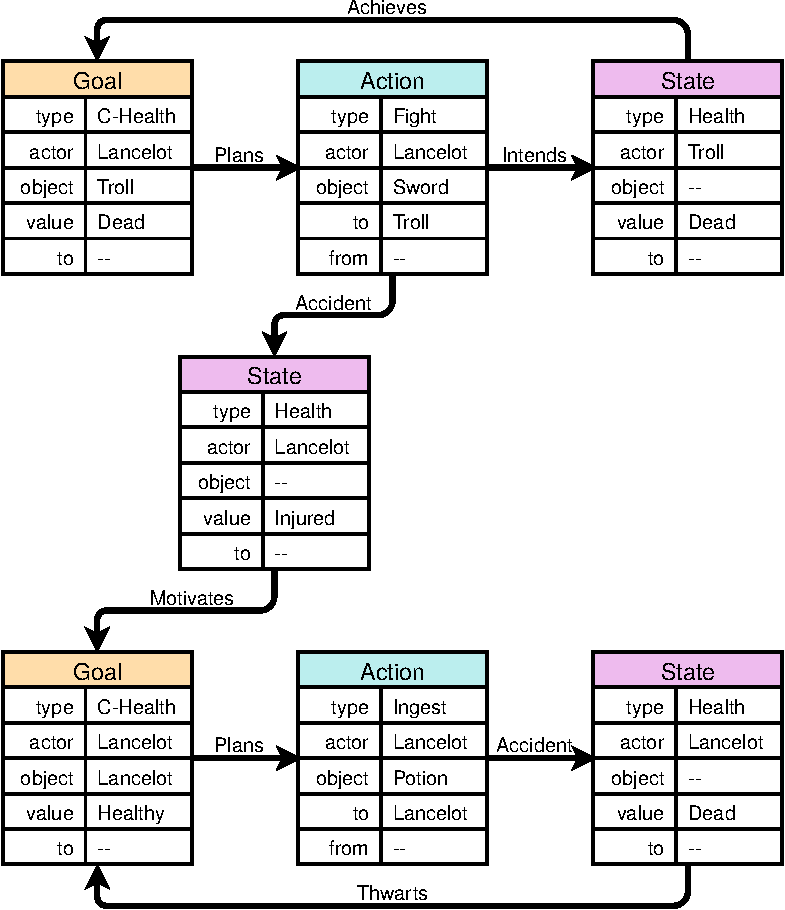
\includegraphics[width=\textwidth]{fig/cropped-story-graph.pdf}
  \caption[Example Skald story graph]{An example of a \skald/ story graph. It represents a story where Lancelot plans to kill a troll, attacks it with his sword and kills it, but becomes injured. After that, Lancelot wants to heal himself so he drinks a potion, but the potion kills him instead.}
\label{fig:story-graph}
\end{figure}


\minstrel/'s story graphs are directed graphs where each node is a conceptual dependency schema and edges are relations between these.
%
The four core node types are \gng/, \gna/, \gns/, and \gnb/ nodes, and they are usually found in \gng/-\gna/-\gns/ triangles linked by \gep/, \gei/, and \gea/ links.
%
Essentially, these \gng/-\gna/-\gns/ triples each represent a single event (along it its motivation and outcome) and they are linked to each other when the \gns/ of one triple has a \gem/ link to the \gng/ of another.
%
Within each node, the details of a particular \gng/, \gna/, \gns/, or \gnb/ are represented using conceptual dependency schemas, as shown in \cref{fig:story-graph}.


A few of the stories from \minstrel/'s original library are described in Turner's dissertation, but Turner's complete library was not available to us.
%
Because of this, we created our own ad-hoc story library by hand-authoring several stories that we thought would provide interesting source material.
%
One of the things we learned from this was that \minstrel/'s story library must be carefully managed to avoid generating malformed stories (this point is discussed in more detail in both \citep{Tearse2012} and \citep{Tearse2014}).
%
In particular, whenever there are multiple ways to represent the same concept in terms of story graph nodes, if different stories in the library use different encodings, the results of the imaginative recall process may be poor.
%
The same was true of \minstrel/'s starting templates: the templates had to match the story library closely in order to generate sensible stories.


\section{Author-Level Plans}

\minstrel/'s author-level plans are essentially black-box code fragments that modify a story during construction.
%
Each plan is invoked in response to an author-level goal (ALG) and can itself add new ALGs to the current generation process.
%
There can be multiple plans which can satisfy a single goal, in which case they are tried in a fixed order until one is found whose preconditions are met.
%
ALGs are stored in a priority queue, and if a selected plan fails to achieve the current goal, that goal is re-enqueued at a lower priority level (until it falls below a priority threshold at which it is marked as permanently failed).


This system allows the results of one plan to inform the operations of another when they both consider overlapping regions of the growing story graph.
%
Once all goals have been achieved, the story is considered finished.
%
The first goal of the system (called simply ``tell story'') is invoked after a story template has been imported, and it assigns both an ``instantiate'' and a ``check consistency'' goal to each node in the imported template.
%
The plans invoked to achieve these goals are responsible for most of the generated story, although there are a few plans which run under certain conditions that add additional nodes to the imported template as opposed to simply filling in empty schema fields.


One category of these template-expanding plans is the ``make-consistent'' plans.
%
These are triggered by consistency goals that arise when consistency-checking plans (triggered by the ``check consistency'' goals added by ``tell story'') find an inconsistent node.
%
For example, the \texttt{Check\abr/Goal\abr/Consistency} plan (which satisfied the ``check consistency'' goal for \gng/ nodes) might find a goal which is lacking a motivating state.
%
In this case, it could trigger the \texttt{Make\abr/Consistent\abr/Motivating\abr/State} plan, which adds a new \gns/ node linked to the \gng/ node by a \gem/ edge and adds a new ``instantiate'' ALG targeting the added node.
%
In this manner, the original story graph can be expanded during generation; \minstrel/ is not simply a complicated mad-libs system.


Although \minstrel/ and \skald/ both contain more than 20 ALPs, the single ALP that is responsible for most of the story content generated is the \texttt{General\abr/Instantiate} plan.
%
This plan is quite simple at the code level: it looks at the node in consideration along with its neighbors in the story graph, and asks the imaginative recall system to fill in the node based on the story library.
%
Of course, the operation of the imaginative recall system (\minstrel/'s case-based reasoning engine) is quite complex, and it is mostly responsible for the creative aspects of \minstrel/'s stories.


\section{Imaginative Recall}

Turner's goal in developing \minstrel/ was to demonstrate the creative potential of imaginative recall, and in particular, how it could recreate elements of of human narrative creativity.
%
Working with stories represented in terms of graphs of story schemas as described above, imaginative recall makes new stories using a story library by taking an incomplete story fragment and filling it in using a similar scene from the story library.
%
For example, a scene where a knight slays a dragon might be recalled when building a story in which a troll is killed, filling in a knight as the protagonist in the new story.
%
Intuitively, imaginative recall recognizes trolls and dragons are similar because they are both monsters, and so the scene where the knight slays the dragon is appropriate source material for the new story.


\begin{figure}[!t]
\centering
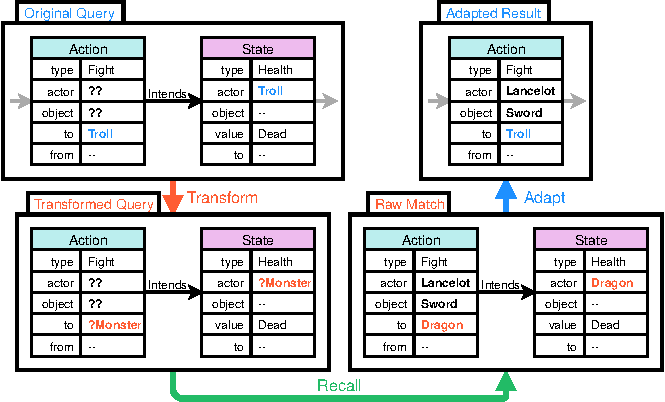
\includegraphics[width=\textwidth]{fig/cropped-im-example.pdf}
\caption[Imaginative recall example]{An example of imaginative recall using a Transform Recall Adapt method (TRAM). The original query (top left) must be Transformed (bottom left) before a match can be Recalled from the story library (bottom right). The match is then Adapted to fill in the query's target node (context nodes are discarded). Note that each empty slot is potentially connected with others in the graph, so that when ``Lancelot'' is chosen as the actor here other slots corresponding to that same actor will also be changed to ``Lancelot.''}
\label{fig:im-example}
\end{figure}


Imaginative recall actually works via a three-step recursive process: Transform, recall, and adapt.
%
First, an input query is transformed so that it can more easily match story fragments from the story library.
%
Second, a matching fragment is picked out from the library.
%
Finally, the matching fragment is adapted so that it matches the context of the current story.
%
In \cref{fig:im-example}, the query is a scene in which a troll is killed.
%
This is represented as an \gna/ node liked to a \gns/ node with an \gei/ link.
%
The \gna/ node specifies that the type of action is ``fight,'' and that a troll is the target, but the actor and tool in this case are still unknown (otherwise the story fragment would already be complete).
%
The \gns/ node specifies that the troll has a health value of ``dead,'' and it doesn't have any unknowns.


Using this query, the imaginative recall system begins by searching for a direct match in the story library: a graph fragment in which all of the fields match with the query (for unknown fields of the query, any value can match).
%
Usually, there is no exact match, as would be the case here if the story library didn't contain any stories about trolls.
%
At this point, the system would begin to consult its library of Transform Recall Adapt Methods (or TRAMs).
%
Each TRAM specifies a specific transformation of a query, along with the steps needed to undo that transformation during the adapt step.
%
Various TRAM selection strategies are possible, including anything from random selection to exhaustive search through the space of possible TRAM applications.
%
Because multiple TRAMs can be applied to a single query, there's effectively a search space of TRAM applications branching out from each starting query, and somewhere within that space (hopefully) is a query that has an exact match with a fragment in the story library.
%
Ultimately, the odds of a match increase as more TRAMs are applied, because each TRAM tends to generalize the query.


Coming back to our example, in the case of the troll being slain by an unknown actor, one available transformation is the ``GeneralizeActor'' transformation.
%
This TRAM says that a specific actor, like ``a troll,'' can be replaced with a generic actor of the specific actor's type (using a simple type ontology of actors).
%
In this case, the TRAM replaces all occurrences of the troll in the query fragment with ``a generic monster.''
%
After transformation, the new query is checked against the story library, and this time, there's a result: the scene where Lancelot the knight kills a dragon now matches our fragment, because the dragon can match ``a generic monster.''
%
Having Recalled a scene from the story library, the Adapt step is triggered.
%
In this case, the adapt part of the ``GeneralizeActor'' TRAM indicates that the actor which matched the generalized actor from the story library scene should be replaced by the actor that was generalized.
%
So the fragment from the library in which a knight slays a dragon is adapted by replacing the dragon with our specific troll.
%
If multiple TRAMs had been necessary to find a match, their adapt steps would all have been applied in reverse order.
%
The adapted story fragment can be incorporated into the story, in this case our result is that a knight kills the troll with his sword (see \cref{fig:im-example}).
%
The TRAM process has eliminated all of our initial unknowns, and this story fragment is now completed; the ALP system takes over again to select a new place fragment for imaginative recall.

\section{\minstrel/'s Potential}

The promise of imaginative recall and the TRAM system is that TRAMs can capture how story scenes can be similar to one another, and then any corpus that can be turned into a story library can become a source for generating new material.
%
Turner acknowledged that some content-specific TRAMs might be needed, and some specific to his Arthurian domain were included in \minstrel/, but these were a minority.
%
And Turner demonstrated that the TRAM system could create stories that the system had never seen before: it didn't just regurgitate what was in the story library.
%
For example, \minstrel/ was able to ``invent'' the concept of suicide by taking a scene where someone was killed and ultimately filling in the killer and the victim with the same person.
%
Because of the kinds of information embedded in \minstrel/'s story graphs, this process isn't just chaos either: \gng/ and motivating \gns/ nodes constrain how their neighboring \gna/ nodes are filled in and enforce some semblance of believability.


However, despite the potential of \minstrel/'s imaginative recall process, it is fundamentally not robust.
%
When building \skald/ we imagined that after providing a new story library containing roughly a dozen stories and doing some minor tuning, we'd be able to have \skald/ generate dozens to hundreds of new stories that included significant variations.
%
Unfortunately, what we found was that the authoring of the story library, the story templates, as well as the particular TRAMs and ALPs all had to be carefully balanced against each other to avoid nonsensical results.
%
In Turner's dissertation, in fact, he mentions a trial run where \minstrel/ is asked to generated stories repeatedly, in which the coherence of the stories breaks down after only 6 reasonable results.
%
So rather than a robust generation engine with the capacity for creative feats, \minstrel/ is a carefully balanced system designed to demonstrate the possibility of such feats.
%
The process of generating interesting stories while avoiding nonsensical ones using \minstrel/ inevitably involves looking at its output and altering the ALPs, TRAMs, and/or story library to correct errors.


\section{Problems with \problemplanets/}

\label{sec:problem-planets-problems}

In fact, this is exactly the issue that we ran into when we tried to build \problemplanets/, a choose-your-own-adventure-style game about climate change that was going to use \skald/ as a narrative generation engine.
%
Brandon Tearse and I teamed up with Aaron Reed to work on the project, which was the first major project where we attempted to put \skald/ to use.
%
Our plan was to set up some domain-specific ALPs and TRAMs for \problemplanets/' domain (a science fiction domain in which the protagonist travels from planet to planet solving climate-related problems on each) and then have Aaron (a noted author of interactive fiction) create a story library that we'd use to generate new stories for each player.
%
Given this design, \skald/ would have to be capable of generating stories unsupervised: we'd be able to tune the system by changing the library or adding ALPs and TRAMs up to release, but at that point it would ideally be able to produce stories we'd never seen before which were nevertheless coherent and interesting.


What we discovered during this process was that \skald/ alone was incapable of consistent unsupervised generation.
%
No matter what we did, \skald/ produced internally inconsistent or otherwise incoherent stories within the first dozen or so it generated in a batch.
%
This was consistent with Turner's result of 6 stories in a run before incoherence of course, but our efforts to control \skald/ led us to the conclusion that we needed to go beyond the imaginative recall framework to achieve better consistency. 
%
In particular, we explored the idea that expanding the story library might give \skald/ more reach, but the opposite turned out to be true: expanding the story library only gave the TRAM system more room to make mistakes.


Ultimately, we turned to the ALPs to fix things.
%
When asking \skald/ to generate a batch of stories in the \problemplanets/ domain, we would observe broken outputs and try to identify patterns.
%
Sometimes, a single story or group of stories in the story library could be re-written to eliminate a problem (this was often the case when different stories in the library used the same pattern of nodes in slightly different ways, and \skald/ crossed these senses during recall).
%
But this meant that Aaron had to be extremely careful in authoring stories for the library, and in particular, the effort of maintaining the library's internal consistency grew quadratically with the size of the library.
%
Furthermore, problems that couldn't be pinned on specific stories were patched using ALPs that checked for and attempted to fix them.


Although Turner did include a few consistency-checking ALPs in \minstrel/, as we began to add more and more of them to \skald/, we realized that imaginative recall alone was no longer a driving force for story consistency.
%
Our architecture was shifting towards one in which imaginative recall supplied creative but often too-much-so results, and a complex system of rules implemented by a tangle of ALPs tried to force these results to be consistent.
%
Effectively, we were trying to write a programmatic definition of what made a story consistent within the ALP system.
%
Ultimately, this problem is fundamental to case-based approaches to story generation: either the case library must be rigorously maintained and developed to account for the intricacies of how retrieved cases are joined into a story, or some other system must fix up mis-matched cases after recall.
%
In either case, a limiting factor emerges: either the effort required to maintain the story library, or the system's ability to understand and thus repair mis-matched story content.


Additionally, we wanted the stories to be interactive, and so we decided to generate choices by simply having the story graphs branch and allowing the user to select a path when this happened.
%
We quickly found that this approach required careful hand-selection of branching points to make the choices sensible.
%
Only at very specific points in a story is it appropriate to present choices to the player, and the range of options that are reasonable is tightly constrained.
%
For choices to be dynamically generated, a strong model of character motivation is necessary, so that options can include a set of motivated actions without including unmotivated or irrelevant ones.
%
Furthermore, different options at a choice point can't be generated sequentially by a system designed for generating linear stories.
%
Instead, the system must be aware that all of the options are presented to the player at once, and generate the entire set of options taking this into consideration.


As we struggled with these difficulties in building \problemplanets/, I came to the conclusion that focusing just on rules of story consistency would be more productive.
%
Seeking to build a story generator that could provide robust variation and also deal with embedded choices, I turned to answer-set programming (ASP), which would allow me to write rules of story consistency as logical statements and let a solver use them to generate concrete stories.
%
In particular, encoding consistency rules as logical formalisms to be obeyed rather than a complex structure of imperative consistency-checking procedures was much more natural.
%
In addition, building a new system would allow me to address from the start the issues with choice generation that I had observed in \problemplanets/.
%
Thus the idea for \dunyazad/ was inspired by the difficulties of \problemplanets/.

% Dunyazad:
\chapter{Choice Poetics}

\label{ch:choice-poetics}

\Footnotetext{~}{Note: a preliminary discussion of some of the material in this chapter can be found in \citep{Mawhorter2014}.}

The aim of this chapter is twofold---first, to establish a framework for talking clearly and precisely about choices and their outcomes, and second, to introduce a method for analyzing choices based on how they relate to player goals.
%
Choice poetics should be able to address questions like: ``What is it about a choice that makes some players feel regret after picking a particular option?''
%
This chapter attempts to establish terminology and formal perspectives that can be used to talk about choices, but it's far from a ``complete'' theory of choice poetics: it only deals with explicit, discrete choices, for example.
%
Some parts of the theory are more developed (those that supported and were influenced by the development of \dunyazad/), but the ideas here are just the beginning of an in-depth study of narrative choices.


Note that here I define ``poetics'' broadly as the compliment of hermeneutics: if hermeneutics is the study of the meaning of a text, poetics can be understood as the study of its non-meaning-related qualities, such as the emotions or themes it evokes.
%
Poetics deals with the feelings that a player has before, during, and after making a choice, including simple feelings like the impression that a choice is difficult to make, but also complex feelings like regret.
%
It is also concerned with how these feelings help a work express themes or otherwise enhance the player's experience of a narrative, although the work presented here focuses mainly on the specifics of how choice structures engender feelings in the players who experience them.


\section{Inspirations}

\Cref{ch:related-work} contains a full review of literature related to choice poetics, but some of the most relevant sources are worth reiterating here.
%
While choice poetics clearly has roots in the work of Aristotle \citep{Aristotle1917} (and more recent narrative formalists like Freytag \citep{Freytag1894} and Barthes \citep{Barthes1975}, to name only a few) choice poetics is also inspired by investigations into the psychology of both reading and decisions.
%
In the first camp, psychologists have studied specific narrative effects such as transportation \citep{Green2000}, surprise \citep{Iran-Nejad1987}, and identification \citep{Oatley1995}.
%
In the second camp, researchers have studied how things like framing \citep{Tversky1981,Tversky1993}, and personality \citep{Schwartz2002} affect decisions and preferences.


Including craft wisdom from places like the Choice of Games development blog \citep{ChoiceOfGamesGameDesignCategory}, existing sources already contain a lot of information about how narrative choices function.
%
However, much of it is focused on either linear narratives or real-world choices, and the resources that do explicitly deal with narrative choices lack a solid theoretical foundation.
%
Some of the work of this chapter is therefore synthesizing this existing information into a theory concerned primarily with discrete, explicit choices in narrative contexts.


\section{Modes of Engagement}


In developing a theory of choice poetics, one must respect the lessons of the development of traditional poetics.
%
In particular, modern scholars have largely rejected ``objective'' narrative analysis and concluded that the experience of the individual reader must be taken into account.
%
Unlike Aristotle, who stated authoritatively what was good and bad about this drama or that, modern narrative scholars will analyze a work from a particular perspective, without claiming that this perspective is universal, perhaps performing a feminist or Marxist reading of a novel to see what insights a particular lens has to offer about the work.


Choice poetics must also respect the perspective of the reader, but it is in a slightly different position, as its readers are also players.
%
Insofar as the narrative that contains choices is experienced through the fabric of a game, the reader/players (henceforth players) are stepping into the magic circle of the game \citep{Huizinga1949} and intentionally taking on certain attitudes.
%
A narrative experienced within the framework of a game thus implicitly biases the attitudes of its readers, for example by setting up a score counter which players can try to maximize.
%
Counter-play is of course possible and important, but even counter-play is influenced by the rules of the game by virtue of being set against them.
%
The formal structures of the game rules that accompany a narrative-with-choices thus allow the theoretician to make an educated guess about the attitudes of players interacting with a piece.


There are still a range of attitudes that players can take on, however, and some understanding of this range is important before any analysis of choices in a narrative.
%
This range of attitudes has to some degree been studied by others interested in player types, although such studies are mostly focused on games without regard to narrative.
%
From simple binary ``casual/hardcore'' distinctions to more complex typologies such as Bartle's ``achievers,'' ``explorers,'' ``socializers,'' and ``killers,'' player type classifications to some degree incorporate notions of player intent or attitude \citep{Bartle1996}.
%
However, player type classifications also focus on player actions or approaches within the game, for example a distinction between those who enjoy stealth or direct combat more.
%
These player content preferences are as important as any other player preferences when it comes to how players approach choices, but they're less important than player motivations, which establish entire contexts within which preferences can be expressed.
%
For example, if one's motivation to play is a desire to act out a role, one's preferences might be expressed in terms of the kind of role one is trying to act out.
%
If one's motivation to play is to score points, on the other hand, preferences might be expressed in terms of different strategies for doing so.


The idea of ``modes of engagement'' captures these different player motivations.
%
Modes of engagement are different ways in which a player can approach a game.\footnote{%
Note that the idea of modes of engagement is not unique to games: different audience approaches have been acknowledged as important in areas such as education and music composition \citep{Langer1995,Brown2001}.}
%
At this point it is important to note that modes of engagement are neither exclusive nor permanent: players often engage in several modes at once (to varying degrees) and may change their modes of engagement during the course of play.
%
The modes of engagement presented here are also not intended to be comprehensive: these are some of the most common modes, but others may be possible and even the norm for certain games.
%
All of that notwithstanding, consideration of the mode(s) of engagement that players bring to a work is the first step in analyzing the choice poetics of a work.


This can take the form of assuming a particular mode: much as one can perform a feminist reading of a novel, one could perform a power-playing playthrough of a game.
%
This could also take the form of analyzing the game itself to determine which mode(s) of engagement it encourages and rewards.
%
It could even take the form of a qualitative study of actual players, to determine which mode(s) of engagement they are employing.
%
In any case, an analysis of choice poetics that does not consider modes of engagement is incomplete.


\Cref{tab:modes-of-engagement} lists some of the most common modes of engagement, and gives examples of decisions that employ them.
%
The last column references Nick Yee's work on motivations for play in massively-multiplayer online role-playing games as a comparison \citep{Yee2006}.
%
The grouping of Yee's motivation components into these modes of engagement has to do with a difference in focus: Yee is focused primarily on aspects of play, including a strong focus on online social interaction, whereas choice poetics is interested primarily in single-player offline engagement with an emphasis on narrative.
%
For example, Yee makes fine distinctions between different motivations grouped into the ``power play'' category here, but from a choice poetics perspective, whether someone is trying to maximize score or compete with an opponent doesn't matter, because both motivations are equally orthogonal to the narrative, and thus they have a similar effect on the player's experience of the narrative.


\begin{table}[!p]
\begingroup
\renewcommand*{\arraystretch}{1.5}
\begin{tabular}{>{\raggedright}p{5.5em}>{\raggedright}p{10em}>{\raggedright}p{9.8em}>{\raggedright}p{6.6em}}
\toprule
\textbf{Mode} & \textbf{Decision Process} & \textbf{Example} & \textbf{\citep{Yee2006}} \tabularnewline
\midrule
\textbf{Avatar Play}%
& Decide as if you were in the character's situation.%
& When picking a pet, pick the cat because you like cats.%
& Role-Playing, Customization, Escapism \tabularnewline
\textbf{Role Play}
& Decide in order to act out a persona.
& Choose the wizard character class because you want to play a shy, bookish person.
& Role-Playing, Customization, Escapism \tabularnewline
\textbf{Power Play}
& Choose options that advance game metrics like score, beating other players, or quick completion.
& Sacrifice an ally to obtain a powerful item because it helps you beat the game more quickly.
& Advancement, Mechanics, Competition, Teamwork \tabularnewline
\textbf{Explora-tory~Play}
& Choose options to see what will happen.
& Turn away from the path of your quest to explore the world.
& Discovery \tabularnewline
\textbf{Social Play}
& In a multiplayer situation, choose options because of social considerations.
& Turn down a high-level quest in order to accompany your friend on a lower-level quest.
& Socializing, \newline Relationship \tabularnewline
\textbf{Analytical Play}
& Make decisions in order to analyze the work.
& Repeatedly load a saved game to explore every option at a choice.
& \emph{none} \tabularnewline
\textbf{Critical Play}
& Make decisions as performance to deconstruct or criticize a work.
& Drive your character into poverty in order to demonstrate a game's biased depiction of the poor.
& \emph{none} \tabularnewline
\bottomrule
\end{tabular}
\endgroup
\caption[Modes of engagement]{Some common modes of engagement.}
\label{tab:modes-of-engagement}
\end{table}

Although modes of engagement are important to choice poetics, in my work with \dunyazad/ I have not given them great attention: \dunyazad/ encourages avatar play and all of its evaluations assume that players will engage primarily in this mode.
%
Extending \dunyazad/ to support power play and role play better, and to account for these possible approaches when evaluating choices, would be a very interesting line of future work.
%
Developing \dunyazad/ in that direction would allow it to be used as a tool to study modes of engagement in more detail.


\section{Dimensions of Player Experience}

When using choice poetics to analyze a narrative or even just a single choice, one must consider the range of expressiveness of narrative choices.
%
Aristotle devoted much of his analysis of emotion in \work{Poetics} to tragedy and the heroic epic as these were traditional forms in his day, but the full range of poetic effects is very broad, and includes both momentary impressions such as a single phrase that provokes disgust, and overall feelings, such as sympathy for a tragic figure.
%
To some degree, more complex effects depend on simpler ones, for example when an overall experience of sympathy depends on many individual positive evaluations of a character, along with negative reactions to bad things that happen to that character.
%
Of course, once choices are involved, the repertoire of effects is expanded, and it's important to have some understanding of what poetic effects a choice can possibly have.
%
Although no summary of possible poetic effects could hope to be complete, I have tried to list here a collection of important high-level aspects of a narrative experience that are strongly influenced by choice structures, including some which I believe are unique to narratives that contain choices.


\begin{table}[!p]
\begingroup
\renewcommand*{\arraystretch}{1.5}
\begin{tabular}{>{\raggedright}p{5.6em}>{\raggedright}p{13.9em}>{\raggedright}p{13.5em}}
\toprule
\textbf{Dimension} & \textbf{Description} & \textbf{Potentially Supported By} \tabularnewline
\midrule
\textbf{Immersion} & The degree to which the player's attention is focused exclusively on the game. & Outcomes that are believable given options; option coverage of desired actions. \tabularnewline
\textbf{Identifica-tion} & How comfortable the player feels in the role they play as their avatar. & Options that support player self-expression. \tabularnewline
\textbf{Transpor-tation} & The degree to which a player thinks in terms of the game world rather than the real world. & Choices which force the player to reason from a character's point of view. \tabularnewline
\textbf{Agency} & Alignment of player goals with game affordances. & Transparent choices where outcomes align with player goals.\tabularnewline
\textbf{Influence} & Degree to which the player feels they influence in-game events (even if they do not control them). & Choices where outcomes are divergent and impactful. \tabularnewline
\textbf{Autonomy} & The player's ability to choose and pursue a variety of goals at their own discretion. & Choices between goals rather than between methods of pursuing a fixed goal; non-exclusive outcomes. \tabularnewline
\textbf{Responsi-bility} & Player feelings of responsibility for the actions of their avatar. & A mix of intentional outcomes that are good for and bad for other game characters. \tabularnewline
\textbf{Regret} & Player feelings of regret for an in-game decision. & Negative outcomes that result from tempting options but which are still believable. \tabularnewline
\bottomrule
\end{tabular}
\endgroup
\caption[Dimensions of player experience]{Some aspects of player experience that are influenced by choice poetics, along with hypotheses about what kinds of choices might support them.}
\label{tab:dimensions-of-experience}
\end{table}

\Cref{tab:dimensions-of-experience} provides a brief overview of these important dimensions of player experience.
%
Except for identification, transportation, and immersion, each of these possible poetic qualities are unique to interactive narratives: without choices, they simply aren't possible.
%
Because of this, figuring out how choice structures contribute to these effects 
is an important task for choice poetics.
%
Of course, some of these effects, like agency, have already been extensively studied, often in broader contexts than just choice-based interactive narrative.
%
But it will still be important to understand how choice structures specifically contribute to these poetic qualities.
%
What follows is a preliminary analysis of each quality, based on craft wisdom and existing studies of games and real-world choices.

\begin{itemize}
\item \textbf{Immersion}---There are several different phenomena that the word immersion can refer to in games, including sensory immersion, mechanical immersion, and narrative immersion (see \citep{Ermi2005}).
%
Narrative choices of the kind studied here bear most on narrative immersion, although they could also be a source of mechanical immersion in some cases.
%
Immersion goes hand-in-hand with effects like identification and transportation.
%
Although counting immersion as a poetic quality discounts the role of the reader to some degree, immersion isn't independent of the structure of a narrative either.
%
In particular, it is possible for a narrative (choice-based or otherwise) to disrupt player engagement when it contains contradictions or otherwise complicates the reader's ability to understand it (see e.g., \citep{Douglas2001}).
%
This is particularly relevant when choices become involved, as they can easily become a source of frustration, either because the player wants to take an action which isn't provided as an option, or because the player views an outcome as inconsistent with the option that led to it.


\item \textbf{Identification}---Identification in traditional narrative is a key property and is heavily influenced by the actions and attitudes of characters (see e.g., \citep{Feilitzen1975,Oatley1995}).
%
In narratives that include choices, the player usually has some control over the actions of one or more character(s), although this control is often incomplete, especially when it comes to attitudes rather than actions.
%
This degree of control can enable a different type of identification in which the player actually assumes the psychological perspective of a character, as opposed to viewing them as a role model (see \citep{Klimmt2009}).
%
Choices could have a big impact on identification if they fail to include options which the player believes are reasonable and which correspond to the choice that the player would be most comfortable with in a given situation, simply because such a situation is an explicit manifestation of a difference between the player and the character (see e.g., \citep{Busselle2009}'s discussion of identification in linear narratives).
%
For example, if the player is a pacifist, but there are never options for negotiating with enemies or otherwise resolving conflicts peacefully, one would expect identification to be hindered.
%
This is complicated by role-playing, however: there is no reason that a player who is a pacifist in real life cannot enjoy the opportunity to play a bloodthirsty character in a game.


\item \textbf{Transportation}---Transportation is the re-centering of a player's perspective from the real world into a fictional world, and is closely linked with narrative immersion (see \citep{Green2000,Green2004}).
%
Although the original research on transportation focused on linear narratives (both textual and visual), a similar phenomenon called presence has been studied in interactive contexts \citep{Witmer1998}.
%
Unlike immersion, transportation is exclusive to contexts that involve fictional worlds.
%
Transportation is also to some degree linked to identification, as when one identifies with a character it becomes easier to project oneself into that character's world (see \citep{Busselle2009} on this point).
%
Again, the believability and completeness of options and outcomes is important when choices come into the picture.
%
In particular, feelings of control and an ability to successfully predict developments have been implicated as contributing to presence (see \citep{Witmer1998}).

\item \textbf{Agency}---Agency has been an important subject for games studies as a feeling uniquely enabled by interactive media (see e.g., \citep{Murray1997,Mateas2001,WardripFruin2009,Mason2013}).
%
The feeling of empowerment that results from being able to achieve one's goals contributes to agency, and an alignment of player goals with player-influenced outcomes is a powerful formula for agency \citep{Mateas2001}.
%
Obviously, such an alignment relates intimately to choice structures, as choice structures establish which outcomes can be influenced by the player and also help set player expectations as to their goals.
%
Given this, opaque choices---where the player is not able to foresee consequences given the setup and options---may decrease agency, because even if an outcome advances player goals, the player may not feel responsible for their success.
%
Additionally, choices where outcomes are tangential to a player's goals can frustrate agency: if you're told to save the princess but then given only choices about which commodities to buy or sell, your ability to proactively pursue your goal has been stifled.


\item \textbf{Influence}---If diegetic agency is an ability to proactively exert control over the story world (see \citep{Mason2013}) then influence is half of that: players' feelings of being influential in the narrative world.
%
Influence is important because fantasies of being powerful are one of the pleasures of both traditional and interactive narratives (see e.g. \citep{Olson2008}).
%
While the experience of agency also requires that players are able to use their influence \emph{proactively} (they must have enough information to make informed decisions, for example), there are plenty of games where the player characters are \emph{influential} but players cannot freely exercise this power to do whatever they choose.
%
For example, a game like \work{Final Fantasy} \citep{FinalFantasy} fully supports player fantasies of being heroic and influential, and if the player makes a mistake this role can be jeopardized, but the protagonists do not have any capacity to control the outcome of their story beyond fulfilling (or failing to fulfill) their fixed destiny.
%
Such a game does not offer players the pleasures of diegetic agency that are uniquely afforded by an interactive format, but it may still offer the pleasure of a power fantasy (a pleasure that is common to both interactive and traditional narratives).
%
Interactivity takes such power fantasies one step further by making them participatory: even when denied agency and thus unable to decide how their character's influence is applied, players are responsible for their character's achievements by virtue of ``pulling the trigger:'' without their input the story cannot move forward, even if that input is a simple ``yes'' or ``no.''
%
Of course, the choices that a player has can serve to advance or undermine this feeling of influence, especially when, for example, a player re-plays to explore multiple paths in a narrative and finds that nothing changes.
%
Divergent outcomes which matter within the story world are critical for maintaining a sense of influence across multiple playthroughs, although a mere suggestion of such can be sufficient when players do not re-play.
%
Important blind choices (where the player must pick an option knowing that the choice will be momentous but uncertain about the exact effects) are a common source of narrative tension which makes players feel influential without giving them a real sense of agency.


\item \textbf{Autonomy}---Autonomy is another relative of agency and influence, and can be summarized as the player's ability to choose and pursue their own goals within a game (see e.g., \citep{Ryan2006}).
%
Some amount of active influence is required to have autonomy, but whereas influence is concerned with outcomes, autonomy is concerned with goals.
%
Autonomy is also distinct from agency: when a game sets up nicely\-/balanced formal and material affordances, agency can be experienced even if autonomy is absent, as in a game like \work{Quake}.
%
The converse is also possible: an overabundance of autonomy can leave players uncertain about what to do, undermining feelings of agency.
%
A game that supports player autonomy provides a play-space within which players can choose their own goals.
%
To the extent that a narrative-focused game can provide this, it will appear more as a space for player-created stories than a fixed story that affords the player some choice.
%
Games like \work{Sim City} \citep{SimCity} and \work{The Sims} \citep{TheSims} provide play spaces within which players can create their own narratives, and this is achieved by offering non-explicit non-discrete choices which give the player a huge amount of options.
%
A lesser degree of autonomy can be present in more linear narratives when the player has choices which affect the goals and priorities of characters within the story.


\item \textbf{Responsibility}---A feeling of responsibility for one's own actions (as distinct from empathizing with a character who feels the burden of responsibility) is something uniquely afforded by interactive narratives (see e.g. \citep{Murphy2013}).
%
Choice structures are key to creating this, and there are several conditions for enabling responsibility.
%
First, the player must be given moral agency within the story world, which means that different outcomes at a choice must have consequences which have morally distinct outcomes.
%
Second, the player must be willing to take responsibility for their actions, and this can be impeded when they feel that the outcomes of their actions were unforeseeable or otherwise out of their control (of course, the feeling of a player who mentally justifies their lack of culpability for an in-game consequence is also an interesting poetic effect).
%
Note that this direct player-responsibility is different from role-played responsibility: it's possible for a player to role-play responsibility even when the actions they are assuming responsibility for were completely outside their control.
%
An example of responsibility (or the shirking thereof) as a poetic effect happens in the game Portal \citep{Portal}, when the player is forced to incinerate their companion cube in order to progress within the game.
%
The complex emotions that arise at that moment are the result of a forced choice between two bad outcomes (being unable to progress and incinerating the companion cube\footnote{Note that this analysis makes assumptions about the player's goals and feelings: some player communities see the companion cube itself as an obstacle worthy of hatred rather than a helper who deserves pity, and so view this choice in a very different light.}), and the moment has emotional resonance later in the game when the player has the opportunity to destroy GLaDOS---the agent which forced the decision upon the player---using similar means.


  \item \textbf{Regret}---Like responsibility, the capacity to make players feel regret is mostly unique to interactive narrative (see \citep{Frome2006,Zagal2009}).
%
Again, in linear narrative it is possible to sympathize and empathize with a character who is feeling regret within the story, but that's a different feeling than personal regret for one's own actions (a book or film might also cause one to revisit a personal regret, but this again is different from being the cause of that regret).
%
As with responsibility, making a player feel regret is quite delicate: the player not only has to achieve some level of transportation and identification, but the choices involved must be structured to resist the player's natural tendency to reassign blame.
%
With a negative emotion like regret, the basic psychological mechanisms of denial are the brain's first line of defence, and so naturally the narrative and choices leading up to a moment of regret will be scrutinized for interpretations that leave the player blameless.
%
In particular, if the player can convince themselves that the game forced them to make a choice that led to a negative outcome, or that the outcome was unforeseeable given the option that led to it, they can often avoid regret.
%
Of course, this process of denial is an interesting poetic effect in its own right, and in some cases is exactly what an author wants (perhaps so they can later force the player to re-examine their denial and admit blame, thus experiencing even more poignant regret).
%
A game like The Walking Dead \citep{TheWalkingDead} forces the player to make many difficult decisions between options with divergent but uniformly negative consequences, and this pattern engenders feelings of desperation and regret.

\end{itemize}


Each of these topics could be (and some of them have already been) the topic of dedicated research.
%
However, they are presented here merely to demonstrate how much there is to learn about choice poetics---\dunyazad/ as a system does not focus on any of these, but rather attempts to get at some simpler phenomena, such as what makes an individual choice obvious, or what is required for a choice to be seen as a dilemma.
%
Patterns of choices with specific properties such as obviousness or unexpectedness of outcomes come together to produce higher-level poetic effects like those described here, and a better understanding of these low-level effects is required in order to aim at higher-level effects.
%
The poetic details that \dunyazad/ actually operationalizes are based on player goals, and the perceived relevance of options and outcomes to them.
%
As \dunyazad/ only reasons about one choice at a time, its logic effectively comprises an analysis technique for examining the basic poetic properties of an individual choice.
%
The next section describes this technique and how a human would apply it to an individual choice within an interactive narrative, while \cref{ch:dunyazad} describes how \dunyazad/ operationalizes this theory, and \cref{ch:option-results,ch:outcome-results} describe how results from two experiments using \dunyazad/ have informed both the theory and the system.

\section{Goal-Based Choice Analysis}

\label{sec:goal-based-choice-analysis}

When authoring a choice or attempting to understand an existing choice, the method of analysis presented here can help tease out how a choice might be perceived by players.
%
This method is grounded in player goals: it views each option and outcome through the lens of what the player wants, and then tries to synthesize this information to understand how an entire choice is perceived.
%
\Cref{fig:choice-analysis-method} gives an overview of the technique described in this section, which consists of seven steps.
%
The basic idea is to carefully break down how the options and outcomes relate to player goals, attempting to consider as many details as possible, and then synthesize those detailed assessments back into high-level assessments of the choice as a whole.
%
The next section describes the methodology used to come up with this analysis method, while the following section describes in detail how a discrete, explicit choice is represented for this analysis, and the seven analysis steps are described in the remaining sections.
%
Finally, an example of the application of the analysis technique is presented in \cref{sec:analysis-example}.


\begin{figure}[!p]
\centering
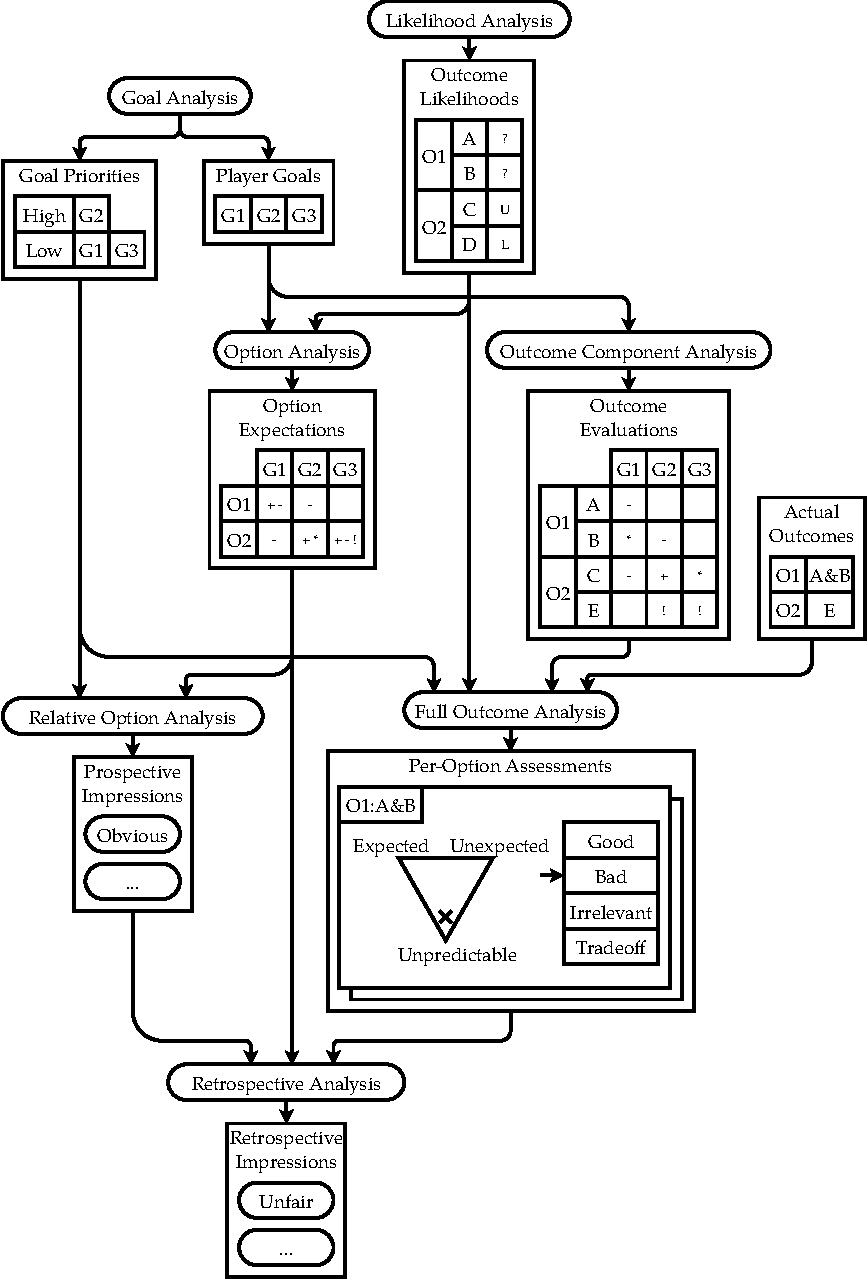
\includegraphics[height=0.92\textheight]{fig/analysis-method-crop.pdf}
\caption[Choice analysis flowchart]{Goal-based choice analysis for a single choice---an overview of the different steps and the information produced.}
\label{fig:choice-analysis-method}
\end{figure}

\subsection{Methodology}

It is worth reiterating the process used for the creation of this analysis technique.
%
A traditional approach might start with a critic observing regular patterns in choices, and invent a rudimentary framework for recognizing these.
%
Such a critic might then attempt to apply this nascent analysis technique to choices in a few well-known games, and then refine it based on these results, continuing this cycle until the method was deemed satisfactory.


Instead, this technique has been developed with reference to the generative system described in \cref{ch:dunyazad}.
%
Using the desire to generate poetic choices as motivation, the question ``What aspects of a choice need to be understood by the system?'' was posed, and a combination of existing systems, craft advice, and theories of both psychology and narrative were consulted to come up with a preliminary answer (see \cref{ch:related-work}; e.g., \citep{Mott2006,ChoiceOfGamesChoiceRules,Shepperd2002,WardripFruin2009}).
%
This initial approach pointed to several important factors: player goals, players' evaluations of the relationship between outcomes and these goals, and things like expectations and likelihoods.
%
These are factors that have been used by existing systems, are the subject of craft advice, appear as variables in psychological studies of decision-making, and are components of theories of interactive narrative.


After identifying these factors as important, the next step was a technical one: using these factors as underlying variables, an answer-set programming framework for representing choices was developed (see \cref{ch:dunyazad}).
%
Technical development proceeded until the system could manipulate these variables and generate rudimentary choices.
%
Of course, the choices it generated at first were flawed, and development of both the theory and the system proceeded through several rounds of revision, using flawed results from the system to motivate elaborations of the theory.


The end product of this methodology for theory development looks a bit different than the results of the traditional approach.
%
For one thing, it is more detailed: because the theory was operationalized early in its development, it naturally contains enough specifics to be evaluated mechanically without necessarily depending on human `common sense' to apply complex criteria.\footnote{%
Of course, humans are still better at applying even the specific criteria of this analysis method, for example when comparing the impact of outcomes they can discern many differences that the generative system cannot.
%
As seen in the following chapters, there is no substitute for humans when it comes to understanding how humans feel; the technique developed here only allows \dunyazad/ to guess correctly in \emph{some} situations, although refinements suggested by experimental results may been able to improve things.
}
%
Another result of the system's unique development path is modularity: each step of the analysis is designed to move from one set of evaluations to another without depending directly on the details of any other step.
%
This modularity is not necessarily beneficial for the resulting analysis technique as a technique, but it does help when attempting to diagnose problems with the system (and thus also with the theory).
%
The separation of modules also allows the theory to be subject to incremental change: an improved method for a specific step could be proposed without needing to overhaul the entire approach.



\subsection{Choice Representation}

\label{sec:cp-choice-representation}

This method is developed primarily for the analysis of explicit discrete choices, and for these choices a detailed breakdown of their structure is possible.
%
\Cref{fig:choice-anatomy} shows how a choice (in this case one generated by \dunyazad/) can be broken down into framing, options, and outcomes.
%
Note that it can be useful to further break down outcomes into individual \emph{outcome components}: individual changes that result from choosing an option which are significant on their own.
%
By doing so, the impact of each outcome component on individual player goals can be analyzed separately, which helps understand outcomes that involve complex trade-offs between multiple goals.
%
Not shown in \cref{fig:choice-anatomy} are unrealized outcome components which nevertheless factor into the choice analysis.
%
For example, if the player were unlucky, the third option might not have resulted in the bandits calming down, and one could even imagine a situation where the bandits might turn on the player.
%
Separate analysis of potential outcome components, such as ``the bandits calm down'' or ``the bandits become angry with the player'' can be used to examine in detail how each option differs from alternatives, even when some outcome components are exclusive of or linked to each other.
%
It's also the case that understanding what the player thinks \emph{might} happen as a result of choosing a given option is just as important as recognizing what does happen as the story unfolds.
%
Finally, this idea of potential outcome components can also help analyze cases where a system is nondeterministic, and the outcomes of a choice vary between playthroughs.
%
Each part of a choice is subject to scrutiny using the methodology presented here, and having precise language to talk about these choice components is necessary for detailed analysis.

\begin{figure}[!p]
\centering
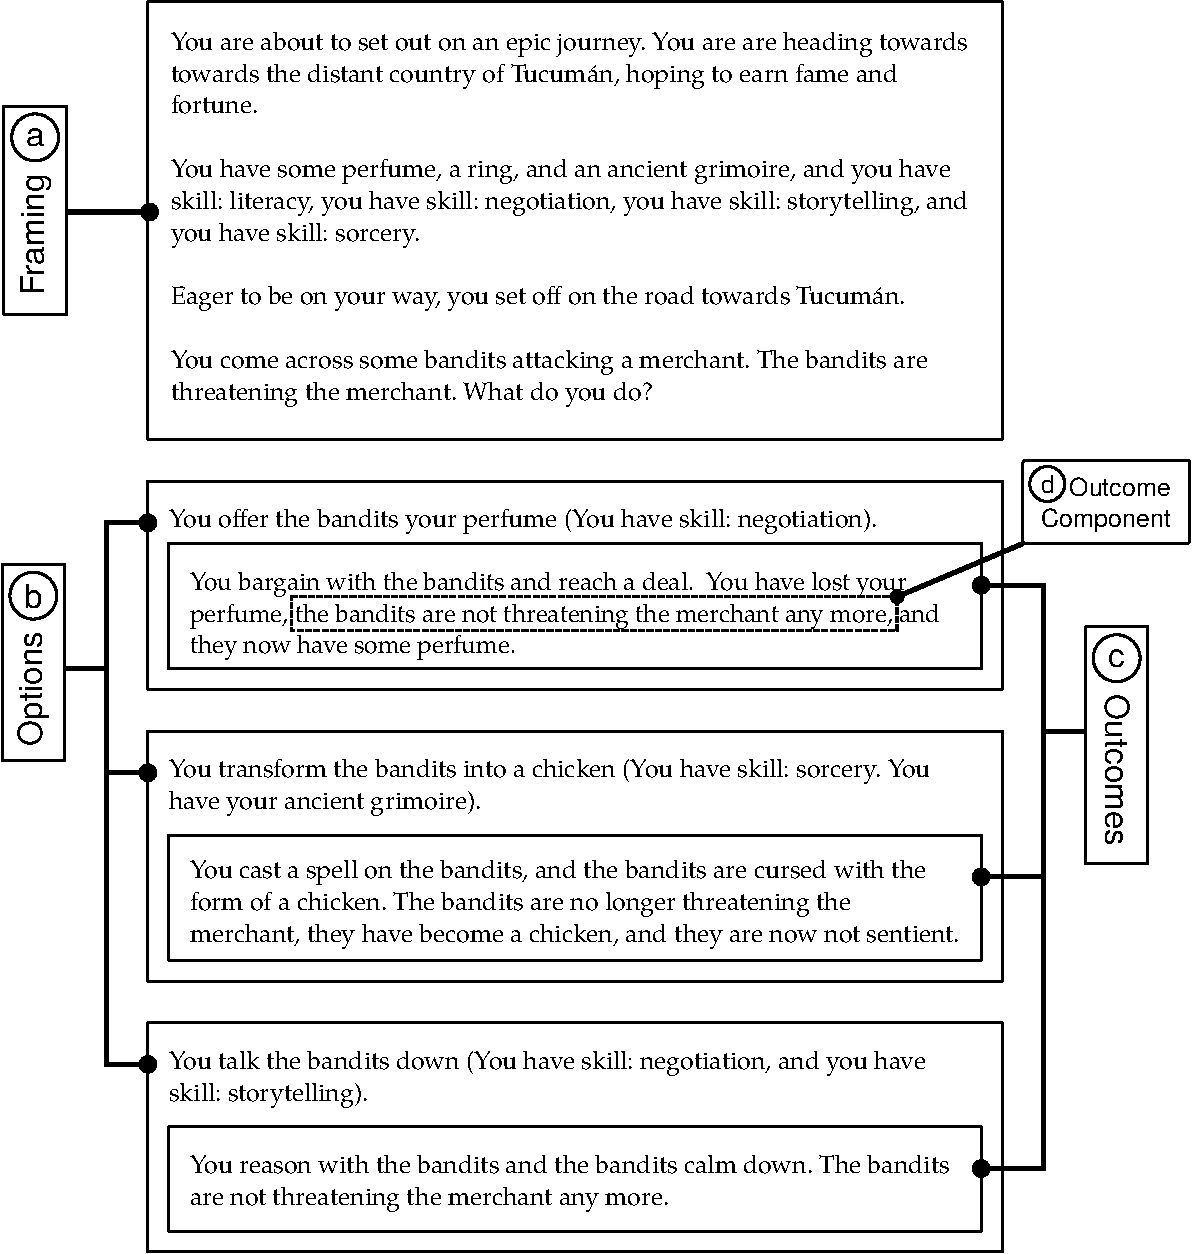
\includegraphics[width=\textwidth]{fig/choice-anatomy-crop.pdf}
\caption[Anatomy of a choice]{%
\setstretch{1.1} % Else the \encircles would stretch only some of the lines
\addtolength{\baselineskip}{0pt plus 1pt minus 1pt}
Anatomy of a choice (using one generated by \dunyazad/).
%
\encircle{a}~Framing---sets up the narrative situation at the choice.
%
\encircle{b}~Options---discrete options available to the player.
%
\encircle{c}~Outcomes---Not initially visible to the player, but revealed after a decision is made.
%
Each option has a single corresponding outcome.
%
\encircle{d}~Outcome components---Individually significant changes that result from picking a particular option.}
\label{fig:choice-anatomy}
\end{figure}


\subsection{Goal Analysis}

\label{sec:cp-goal-analysis}

As already mentioned, poetic analysis of a choice depends on some understanding of the player's approach to the choice.
%
For goal-based choice analysis, this is taken into account by coming up with a list of player goals.
%
Depending on the objective of analysis, there are different ways to come up with this list.
%
One method is to simply list the goals that the analyst themselves would have when approaching the choice.
%
Another is to try to put oneself in the shoes of a particular type of player, perhaps according to one of the modes of engagement listed above.
%
This can be useful for an author trying to figure out how different types of players will perceive a choice: just come up with goal lists corresponding to each player type of interest and perform separate analyses using each list.


In any case, coming up with these lists should take into account not only the desires of the actual or imagined player, but also what aspects of the framing of the choice and previous content encourage which player goals.
%
Based on the options available at previous choices and the narrative content, games can not only encourage certain general modes of engagement, but can establish and encourage the pursuit of specific goals.
%
This encouragement itself often depends on a player's mode of engagement to function as intended, however.
%
For example, game rules directly establish goals for power gamers, but players who have a different mode of engagement may not care about those goals.


If an important goal is missing from the goal list, the entire analysis may be skewed, so it's important to consider the full set of probable player goals.
%
On the other hand, it's always possible to come back to the goal analysis if one realizes during a later step that there's an additional goal that might be relevant. 
%
This is not uncommon, as the particular set of options and outcomes at a choice  determines which goals are relevant.
%
However, part of the point of performing goal analysis before even considering the structure of the choice in question is to avoid bias.
%
This also means that the results of goal analysis can be re-used when analyzing multiple choices.
%
Of course, player goals may change over the course of a game, and this must be taken into account, but performing a full goal analysis from scratch for each individual choice is generally not necessary.


Besides just listing player goals, a goal analysis must give some notion of their relative priorities.
%
This can be as simple as sorting the goals into ``high'' and ``low'' priority tiers, but a more detailed representation of priorities can also be used.
%
This priority information is used when combining information about multiple options and outcomes during the relative option analysis and full outcome analysis steps.
%
Because goal priorities are even more volatile and difficult to estimate than goals themselves, sometimes it's simplest just to wait until the later analysis steps to consider goal priorities, as there will likely be only a few specific goals (those relevant to the choice in question) for which priorities actually affect the analysis.


\subsection{Likelihood Analysis}

\label{sec:cp-likelihood-analysis}

The second step of analysis is to figure out which potential outcome components are made to seem likely by the framing and option text of the choice, and assign each component a label of \lbl{likely}, \lbl{neutral}, or \lbl{unlikely}.
%
For each option, this step starts by identifying a set of outcome components that seem plausible, and then figuring out which of those are likely and unlikely.
%
The goal of this step is to identify outcome components that the player can \emph{presume} will result from each option, so if there are actually multiple conflicting likely scenarios (combinations of outcome components), only outcome components present in \emph{all} probably scenarios count as \lbl{likely}.
%
For example, if one option involves rolling a six-sided die, but the player has been given a prophecy that the result will be either a six or a one, then the outcome components associated with rolling a six and those associated with rolling a one are all \lbl{neutral} in this analysis, while outcome components associated with other rolls are \lbl{unlikely}. 
%
Any outcome component that's associated with both rolling a six and rolling a one would still be marked as \lbl{likely}: given the information the player has, they can assume that such an outcome component will happen if they choose to roll the die.


The outcome likelihoods produced by this step are used during option analysis in combination with the list of player goals from the goal analysis to figure out how each option portrays itself as affecting each goal.
%
\Cref{fig:choice-analysis-method} displays these assignments in the `Outcome Likelihoods' box: the choice has two options, `O1' and `O2,' and O1 suggests outcome components `A' and `B,' while O2 suggests outcome components `C' and `D.'
%
Components `A' and `B' are both \lbl{neutral} (indicated by a `?'), while component `C' is \lbl{unlikely} (a `U') and component `D' is \lbl{likely} (an `L').
%
Note that it's possible and even common for the same outcome component to be a plausible result of multiple options, although that situation is not shown in \cref{fig:choice-analysis-method}.


During this step, the actual outcomes of each option are irrelevant; what's important are the cues present in the framing and options that hint at what might happen if an option is elected.
%
This often includes a large body of implicit player knowledge that depends on player experience with a game: players who have played a game already (or even just games from the same genre) may build strong expectations from minimal cues.
%
Much like player goals, potential and likely outcomes from a player's perspective can be difficult to predict perfectly.
%
However, from a designer's perspective, each choice is usually explicitly crafted to present certain outcomes as most salient, and in that case, this step of analysis is mostly focused on double-checking the framing and options to ensure that they highlight the intended outcomes properly.


\subsection{Option Analysis}

\label{sec:cp-option-analysis}

Given the player goals and estimates of likely-seeming outcome components, option analysis proceeds by analyzing how each option seems likely to impact each goal, aggregating information across outcome components at each option.
%
First, all \emph{possible} outcome components are considered, to come up with an estimate of the goals that could possibly be impacted by each option.
%
These evaluations are \lbl{enables} and \lbl{threatens}---which goals each option might possibly advance, and which goals it might possibly impede.
%
In \cref{fig:choice-analysis-method} the `+' and `-' symbols in the `Option Expectations' box are these \lbl{enables} and \lbl{threatens} assignments.


Essentially, these \lbl{enables} and \lbl{threatens} evaluations are produced by considering the impact of each outcome component on each goal.
%
If any possible outcome component of an option could negatively impact a particular player goal, it is said that that option \lbl{threatens} that goal.
%
Likewise, if an outcome component can positively impact a goal, it is said that that option \lbl{enables} that goal.
%
It is possible and even common that an option both \lbl{enables} and \lbl{threatens} the same goal, and of course it's also possible that it neither \lbl{enables} nor \lbl{threatens} a particular goal (or even any goal at all).
%
For example, an option to ``attack the dragon'' presumably both \lbl{enables} and \lbl{threatens} the goal of preserving one's life, as both being killed and surviving are \emph{possible} outcome components (even if one seems more likely than the other).


Besides \emph{possible} impacts of each choice, option analysis is also concerned with \emph{likely} impacts.
%
Using the same procedure, but this time only considering \lbl{likely} outcome components, \lbl{advances} and \lbl{hinders} option expectations are assigned to each option/goal pairing (these are the `*' and `!' symbols in the `Option Expectations' box of \cref{fig:choice-analysis-method}).
%
In other words, when an option's \lbl{likely} outcome component positively impacts a goal, that option is said to \lbl{advance} that goal, and a similar negative impact results in a \lbl{hinders} label.
%
If it's not clear whether an option \lbl{advances} or \lbl{hinders} a goal (perhaps because of multiple conflicting outcome components), neither label should be assigned: the \lbl{enables} and \lbl{threatens} labels should already be present and serve to indicate the possible but uncertain outcome relative to that goal.
%
On the other hand, if contrary indicators are present but one is clearly stronger or much more likely than another, the label more strongly indicated can be assigned, but this should only be done if the player can safely assume that the goal will be affected as indicated, as that is the purpose of these labels.
%
Note that an \lbl{advances} label can only be present if there is an \lbl{enables} label, and similarly a \lbl{hinders} label requires the presence of a \lbl{threatens} label.
%
The combination of \lbl{enables}, \lbl{threatens}, and one of either \lbl{advances} or \lbl{hinders} is common, and indicates an option that will probably advance or hinder a goal but with some risk involved.
%
For example, the hypothetical ``attack the dragon'' option discussed above might not only \lbl{enable} and \lbl{threaten} the goal of self-preservation but also \lbl{hinder} it, if the player believes that being killed is a \lbl{likely} outcome component and that staying alive is not.


The separate analysis of all vs\@. \lbl{likely} outcome components and the four labels that result allow a wide range of choice structures to be accurately described in simple terms, especially when comparing labels assigned between one option and multiple goals.
%
The analysis of all possible outcome components for the \lbl{enables}/\lbl{threatens} labels captures a broad view of option/goal relationships while the \lbl{advances} and \lbl{hinders} labels based on only \lbl{likely} outcome components capture information about the perceived ``most likely scenario.''
%
Patterns across multiple goals (for example a ``tradeoff'' when one goal has an \lbl{advances} label while another has a \lbl{hinders} label at a particular option) are easily recognizable, and this is the basis for the relative option analysis step.


Remember that this step still makes no use of the actual outcomes of an option: it is just concerned with how the player views each option before making a decision.
%
It can also ignore the goal priorities because each goal is considered separately.
%
The option expectations produced by this step are used in the relative option analysis and retrospective analysis steps as a formal representation of how the player views each option.
%
During those analyses more fine-grained evaluations of player perceptions may be required on a case-by-case basis, but the \lbl{enables}/\lbl{threatens}/\lbl{advances}/\lbl{hinders} labels allow such complicated cases to quickly be separated from the simple cases.


\subsection{Relative Option Analysis}

\label{sec:cp-relative-option-analysis}

After producing option expectations for each goal/option pairing, a full-blown analysis of the choice from a pre-decision standpoint can be produced by comparing the options available.
%
A set of prospective impression labels can be used to identify common option structures, and choices that don't easily fit into a known category can be examined more closely.
%
This step uses not only the option expectations from the option analysis step, but also the goal priorities that were produced during goal analysis.


Certain common patterns of option expectations create well-understood prospective impressions.
%
For example, a dilemma has a specific feel, and several types of dilemma can be easily identified by comparing option expectations.
%
If there are exactly two options at a choice, each has overall negative impacts on high-priority player goals (and these impacts are roughly balanced), and each option negatively impacts a different set of goals, then the choice is a classic dilemma.
%
All of this information (besides the balance of impacts) is directly encoded in the goal analysis (priority information) and the option analysis (\lbl{hinders} labels) results, so classic dilemmas are easy to identify using this analysis method.
%
From a design standpoint, it's also easy to identify when an option isn't a classical dilemma and which aspects of that option would need to change to make it one.
%
Given the detailed language of choice analysis it's further possible to describe other kinds of dilemmas: a two-option choice with balanced positive outcomes, or a three-option choice that still has balanced outcomes, or even a tradeoff choice where each option has positive impacts on one of two goals and negative impacts on the other.
%
This is one of the benefits of a detailed analysis technique, in fact: developing the precise language necessary for describing choices formally establishes a framework within which variations on a common pattern can be identified and enumerated.


\begin{table}[!p]
\begingroup
\renewcommand*{\arraystretch}{1.5}
\begin{tabular}{>{\raggedright}p{6em}p{11em}p{16em}}
\toprule
\lbl{Label} & \textbf{Description} & \textbf{Criteria} \tabularnewline
\midrule
\lbl{Depressing} & A choice where no matter which option you choose, there's a goal that's hindered . & Each option \lbl{hinders} at least one top-priority goal. No option should \lbl{enable} or \lbl{advance} any top-priority goals. \tabularnewline
\lbl{Dilemma} & A difficult decision between two strictly negative outcomes. (A particular kind of \lbl{depressing} choice.) & Exactly two options, each of which \lbl{hinders} one of two different top-priority player goals. The priorities of the goals and the severity of the consequences should be balanced and neither option should \lbl{enable} or \lbl{advance} any goals (even low-priority ones). \tabularnewline
\lbl{Empowering} & A choice where every option has a positive impact. & Every option \lbl{advances} a player goal, and may \lbl{threaten} one or more goals but does not \lbl{hinder} any. \tabularnewline
\lbl{Obvious} & A choice that has one option which is clearly better than the rest. & One option that \lbl{advances} a top-priority player goal without \lbl{hindering} any (although it may \lbl{threaten} some), while none of the rest of the options \lbl{enable} any top-priority goals, and each of them \lbl{threatens} some goal. \tabularnewline
\lbl{Relaxed} & A choice that has no impact on any high-priority goals and where no goals are threatened. & There are no option expectations involving high-priority goals (positive or negative), and there are no \lbl{threatens} expectations (and thus no \lbl{hinders} expectations). \tabularnewline
\lbl{Mysterious} & A choice where there is no indication of which option is best or how the outcomes might affect things. & There are zero option expectations, including \lbl{enables} and \lbl{threatens} expectations. \tabularnewline
%\textbf{Uncom-fortable} & A choice where the best option isn't very good, but it's better than the alternatives. & There's one option which is expected to \lbl{enable} an important player goal (but not to \lbl{advance} it), while every other option has some combination of \lbl{threatens} and \lbl{hinders} expectations. The enabling option also \lbl{threatens} and possibly \lbl{hinders} the goal that it \lbl{enables}. \tabularnewline
\bottomrule
\end{tabular}
\endgroup
\caption[Prospective choice impressions]{Several different prospective impression labels, with formal criteria based on option expectations and goal priorities.See \cref{sec:results-prospective-caveats} for a detailed discussion of some of these labels informed by experimental results.}
\label{tab:prospective-impressions}
\end{table}


\Cref{tab:prospective-impressions} gives an overview of some prospective impression labels and the criteria for applying them based on goal priorities and option expectations.
%
Note that the criteria are designed to be sufficient for applying the label, but not necessary---there are certainly some obvious choices which do not meet the strict criteria set out here, but from a design standpoint, if the criteria are met, a choice is almost certainly obvious (assuming also that the goal and outcome analyses are accurate of course).
%
The labels in \cref{tab:prospective-impressions} and their criteria were developed as part of \dunyazad/'s choice analysis component, and some of them (the \lbl{depressing}, \lbl{empowering}, \lbl{obvious}, and \lbl{relaxed} labels) were refined based on experimental results (see \cref{ch:option-results,ch:outcome-results}).


As a preview of those results, one caveat that applies to the \lbl{relaxed} label is that some people will always seek a best possible outcome when given a choice, and thus even at a choice among supposedly positive outcomes, options which appear to lead to \emph{relatively} worse outcomes may be seen as bad options \citep{Schwartz2002}.
%
See \cref{sec:results-prospective-caveats} for further discussion of some extra considerations for applying these labels.


The labels presented here give an idea of how players will feel when faced with this choice before they make a decision.
%
Classic dilemmas, for example, are stressful decisions which are difficult to make: they represent significant negative events and are a source of narrative tension (see \citep{Barber2007a}).
%
In linear narrative, dilemmas and their consequences are commonly used as low points in a story, and are themselves often a result of a character's previous poor decision, in effect serving as extended punishment: the character must not only suffer a negative consequence, but must also choose which consequence to accept, thereby being forced to reflect on their initial decision while agonizing about their present options.
%
Despite being negative moments, dilemmas can also serve as moments of clarity: when a character finally confronts the bad options available to them and makes a decision, this can mark the end of denial about their situation and ultimately the beginning of redemption.


In an interactive narrative, presenting the player with a dilemma can serve the same purposes: to accentuate an earlier mistake and punish the player, while perhaps also establishing a new goal of moving towards atonement.
%
A classic dilemma is a moment of heightened tension, and when a player is forced to make the decision it also represents a pause in the action, although a dilemma where the player has limited time to choose can also be used to accentuate feelings of urgency and haste (\work{The Walking Dead} makes effective use of both kinds of dilemmas \citep{TheWalkingDead}).
%
Additionally, when a player is confronted with a diegetic dilemma, any reasoning about which option is best is done from a point of view within the narrative, which may serve to heighten transportation.
%
At the same time, since diegetic dilemmas can force the player to make an important decision for their avatar and to ``think as'' their avatar, they may promote identification.


Dilemmas can be very fragile, however, because if the goals hindered by the two options are not well-balanced, the choice can become obvious (this impacted the experiments described in \cref{ch:option-results,ch:outcome-results}).
%
A dilemma may also force a player to re-evaluate their priorities, especially when the player goals involved relate to different modes of engagement.
%
For example, if one option hinders a player's ludic goal of becoming more powerful (without necessarily affecting a similar diegetic goal) while another hinders the diegetic goal of preserving the safety of their avatar's ally, many players may simply make a decision to prioritize one mode of engagement (avatar play or power play, in this example) over the other, and thus avoid the dilemma.
%
Of course, a choice like this that forces the player to decide between orthogonal goals can be used intentionally by an author to build divergent experiences for players who presumably prioritize different things.
%
Such a choice not only measures a player's priorities but also probably affects them: human cognitive biases related to self-consistency and rationalization mean (see e.g., \citep{Hall2012}) that once a player commits to a certain set of priorities they are likely to stick with that choice.


A label like \lbl{dilemma} can thus be unpacked into a rich understanding of the poetics of a choice.
%
Beyond assigning such well-understood labels, however, relative option analysis can also find choices which don't strictly conform to any labels, and analyze them on a case-by-case basis.
%
It is often useful to compare a specific choice structure to known structures and focus on the differences.
%
For example, a choice that meets all the criteria for being \lbl{obvious}, but where the best option also \lbl{hinders} a top-priority goal, could be compared to an \lbl{obvious} choice.
%
In this case, the relative merits of the goals \lbl{advanced} and \lbl{hindered} by the best option might mean that the decision is still straightforward, but even so the player may feel some reluctance that a normal \lbl{obvious} choice would not create.
%
Alternatively, because of the \lbl{hindered} goal and despite the \lbl{advanced} goal, an option which \lbl{threatens} some unimportant goal and has no other expectations might be more desirable than the `best' option if the player is risk-averse, creating a very different impression.
%
The relatively narrow labels presented here thus serve as anchor points for the analysis of more complex choices.
%
Of course, it's possible to establish many more clearly-defined labels than those presented in \cref{tab:prospective-impressions}, and doing so is a straightforward way to increase our understanding of choice poetics.


\subsection{Outcome Component Analysis}

\label{sec:cp-outcome-component-analysis}

While the results of relative option analysis give a sense of how a choice is perceived just before the player makes a decision, more work is necessary to understand how a player feels after experiencing an outcome.
%
This begins with outcome component analysis: Using the list of player goals and the actual outcome components at each option (as opposed to the potential components identified during likelihood analysis), a breakdown of the actual impact of each outcome component on each player goal is created (unlike the option analysis step, this step does not aggregate information across outcome components at each option, instead evaluating each outcome component/goal pairing individually).
%
Recall that the option analysis step already summarized how the framing and options of a choice indicated goals would be affected, but during this step, actual effects based on actual outcome components are considered instead of hypothetical effects based on potential outcome components.


An example of this distinction can be helpful: let's say the player has been flung off of a cliff and faces a choice between grabbing a nearby branch to save themselves or grabbing the outstretched hand of their avatar's only child, who is also falling.
%
As presented, the outcomes look grim: sacrifice any hope of saving one's child to save oneself, or catch one's child and at least suffer the same fate.
%
Assuming that the player can't reasonably expect some sort of miracle to save them (even given the full implications of genre conventions, etc.) both options are portrayed to have likely negative impacts on several player goals (assuming an avatar play mode of engagement).
%
But perhaps if the player chooses to grab their child, the actual outcome is that a freak gust of wind blows them both to safety, while if they choose to grab the branch, their child falls and dies.
%
This outcome component of being blown to safety would not appear during likelihood analysis and it would thus not be considered during option analysis, but as it is an actual outcome component, outcome component analysis would evaluate it (see outcome component `E' in \cref{fig:choice-analysis-method}).
%
The goal of outcome components is to analyze the valence of actual outcome components with respect to each player goal, including any components that weren't suggested by the framing and options of a choice.


The method is simple: for each outcome component that actually happens at each option (or when outcomes are non-deterministic, for each outcome component that could happen), estimate its impact on each player goal.
%
The `Outcome Evaluations' table in \cref{fig:choice-analysis-method} that results from outcome component analysis illustrates this, using `$\uparrow$', and `$\downarrow$' for minor positive and negative consequences, and `$\uparrow\uparrow$' and `$\downarrow\downarrow$' for major consequences respectively.
%
Of course, a finer gradation of consequences could be used if desired, and certainly should be employed on a case-by-case basis where specific consequences must be compared, but gross distinctions are often sufficient to analyze straightforward choice structures.


Note that even though the outcome component `C' of outcome `U2' does not actually occur according to the `Actual Outcomes' table, it is still analyzed in this example, perhaps because it might occur depending on the circumstances.
%
In contrast, the suggested outcome component `D' of option `O2' does not appear in the analysis of `O2's outcome `U2,' presumably because although implied as a possibility, it will never actually occur.
%
Outcome component `E' is the opposite: it was not implied, but does occur, and so must be analyzed.
%
There are thus several categories of outcome components: \emph{suggested} components that are hinted at by the framing and option text of a choice, but which may or may not even be possible, \emph{potential} components which are possibilities given a specific decision, \emph{actual} components which actually happen in a given play-through, and \emph{unrealized} components which could have happened given a particular decision but did not.
%
In the example analysis from \cref{fig:choice-analysis-method}, outcome components `A,' `B,' and `C' are both suggested and potential, while component `D' is only suggested.
%
Meanwhile, components `A,' `B,' and `E' are actual, while `C' is unrealized; note that component `E' is not a suggested component.


Depending on the interactive narrative, complex rules may exist that establish what configurations of actual outcome components out of the set of potential outcome components are valid, and the player may or may not be aware of these rules.
%
If analysis is being conducted without a specific playthrough in mind, then in latter stages the different possible combinations of potential outcome components will have to be considered separately, as each may give rise to a different player experience.
%
Of course, player experiences must already be separated based on which option is chosen, but this does add some complexity to the analysis.
%
In the rest of this chapter outcomes are assumed to be deterministic, as that is the case for choices generated by \dunyazad/, and it generally makes analysis much more straightforward.
%
Once an understanding of how each potential outcome component affects each goal is reached, this information can be used to analyze the possible outcomes.


\subsection{Full Outcome Analysis}

\label{sec:cp-full-outcome-analysis}

By combining information from the goal analysis, likelihood analysis, and outcome component analysis steps, as well as information on which outcome components are actual for each option, a full picture of the effects of choosing each option can be assembled.
%
This stage of analysis summarizes some details of earlier stages to make common choice configurations easy to recognize, although for complicated structures these summaries may be insufficient and the results of earlier analyses will need to be used directly by the final retrospective analysis.
%
The goal of this stage of analysis is to establish two main evaluations for each option (and the corresponding outcome components): first, to what degree was the result \lbl{expected}, \lbl{unexpected}, or \lbl{unpredictable}, and second, was the outcome overall a \lbl{good} one, a \lbl{bad} one, a \lbl{tradeoff}, or \lbl{irrelevant}.


The evaluation of expectedness relies on comparing option likelihoods from the likelihood analysis step with actual outcomes.
%
First, however, each outcome component is established as either \lbl{important} or \lbl{unimportant} based on whether or not it affects any top-priority player goals (using actual outcome components, not merely suggested components).
%
Any outcome which is established as an alternative to an important outcome is also important, even if that outcome does not itself interact with a top-priority player goal.
%
When judging expectedness and valence of outcomes, \lbl{unimportant} outcome components are ignored (for a more detailed analysis using graded goal priorities, just factor goal priority into the expectedness and valence judgements as a weighting factor).


Given \lbl{important} outcome components, the results of an option can be said to be completely \lbl{predictable} if every \lbl{important} actual outcome component at that option was identified as a \lbl{likely} component by the likelihood analysis.
%
Options where the \lbl{important} outcome components have a mix of \lbl{likely} and \lbl{neutral} likelihood fall somewhere between \lbl{predictable} and \lbl{unpredictable}, with options where all \lbl{important} components have \lbl{neutral} likelihood are fully \lbl{unpredictable}.
%
If \emph{any} \lbl{important} outcome component was marked as \lbl{unlikely}, however, the results are \lbl{unexpected}, and the same is true if there is an \lbl{important} outcome component that was not a suggested component at all (and thus does not appear in the likelihood analysis).
%
A simple analysis can use these three evaluations as exclusive labels, while a more nuanced analysis might represent the space between \lbl{predictable}, \lbl{unpredictable}, and \lbl{unexpected} outcomes as a continuous triangle as shown in the `Per-Option Assessments' block of \cref{fig:choice-analysis-method} (in this case only the assessment for the first option is shown).


Besides predictability, outcomes have valences, which represent whether they are overall \lbl{good}, \lbl{bad}, or somewhere in-between.
%
Shown in \cref{fig:choice-analysis-method} is a simple \lbl{good}/\lbl{bad}/\lbl{irrelevant}/\lbl{tradeoff} scheme, but finer distinctions can be made within each category (for example whether a tradeoff is generally worth it or not).
%
Essentially, these evaluations summarize all goal impacts of the actual outcome components of an option, taking into account the relative strengths of each impact and the relative priorities of the associated goals.
%
Although this summarization step may muddle things in more complicated cases, it can be helpful for quickly identifying the simple cases: often the results of each option are simply purely \lbl{good} or \lbl{bad} in terms of important player goals, and their impact on the player can be judged accordingly.


By assigning a single predictability value and valence to each option at a choice, it becomes much easier to get an overall picture of how the choice might look in retrospect given a particular decision.
%
Along with the prospective impressions established by the relative option analysis step, these per-outcome assessments are used by the final retrospective analysis step to understand how the player perceives an option after they've made a decision.


\subsection{Retrospective Analysis}

\label{sec:cp-retrospective-analysis}


Retrospective analysis is the final step in the goal-driven option analysis framework presented here, although the results of the relative option analysis step can sometimes be used in isolation.
%
Retrospective analysis complements relative option analysis by providing an understanding of how the player feels after making a decision and experiencing the outcome of a particular option at a choice.
%
Note that further comparative analysis of outcomes would be necessary to understand how a player might view a choice after experiencing multiple outcomes, but the usual case in which a player only experiences a single outcome doesn't need this extra step.


As with the relative option analysis, this step is focused on matching against a set of characteristic option structures.
%
Note that each option is treated independently, although prospective impressions of the entire option set apply no matter which option is under scrutiny.
%
\Cref{tab:retrospective-impressions} lists some retrospective impressions identified during the creation of \dunyazad/ and the formal criteria for each.


\begin{table}[!p]
\begingroup
\renewcommand*{\arraystretch}{1.5}
\begin{tabular}{>{\raggedright}p{5em}p{10em}p{18em}}
\toprule
\textbf{Label} & \textbf{Description} & \textbf{Criteria} \tabularnewline
\midrule
\textbf{Expected Success}
& A predictable outcome that advances player goals.
& The option selected \lbl{advances} a player goal without \lbl{hindering} any, and its outcome is both \lbl{predictable} and \lbl{good}. \tabularnewline
\textbf{Expected Failure}
& A predictable outcome that hinders player goals.
& The option selected \lbl{hinders} a player goal and doesn't \lbl{advance} any, and its outcome is both \lbl{predictable} and \lbl{bad}. \tabularnewline
\textbf{Nice Gamble}
& An option that seemed like a gamble but that turned out well.
& The option selected didn't \lbl{advance} or \lbl{hinder} any player goals, or it both \lbl{advanced} and \lbl{hindered} one or more goals that were approximately balanced. The outcome was \lbl{unpredictable}, but also \lbl{good}. The selected option was not distinctly worse-seeming than any other options. \tabularnewline
\textbf{Bad Gamble}
& An option that seemed like a gamble and did not pay off.
& As above, but with a \lbl{bad} outcome. \tabularnewline
\textbf{Unfair}
& An option that seemed good but had unexpected negative consequences.
& The selected option must be expected to \lbl{advance} at least one top-priority player goal, while not \lbl{hindering} any. It must also have an \lbl{unexpected} and \lbl{bad} outcome. \tabularnewline
\textbf{Miracle}
& An option that seemed like a lost cause but that turned out well against expectations.
& The selected option must be expected to \lbl{hinder} at least one top-priority goal, while not \lbl{advancing} any. It must have an \lbl{unexpected} and \lbl{good} outcome. \tabularnewline
\bottomrule
\end{tabular}
\endgroup
\caption[Retrospective outcome impressions]{Several retrospective impression labels, with formal criteria based on option expectations, prospective impressions, and option assessments. See \cref{sec:results-retrospective-caveats} for some caveats based on experimental results.}
\label{tab:retrospective-impressions}
\end{table}


As with the prospective impression labels, retrospective impression labels are fairly narrow, but ``near misses'' can often be analyzed as a variant of a known case.
%
For example, an option that almost fits the ``bad gamble'' profile but for which there \emph{is} another option that seemed distinctly better has a slightly different feel from a normal bad gamble, but the difference isn't drastic (mainly, the player may place more blame for the failure on their own decision-making than on simple bad luck).
%
A full picture of how player feels after a choice combines prospective and retrospective impressions, for example: An \lbl{obvious} choice at which the player chose the `best' option which resulted in an \lbl{expected success}.
%
Options other than the chosen one can still influence the overall impression, especially by accentuating bad results (when multiple options seemed promising) or good results (when all options seemed bad).
%
Regret in particular is an example of a poetic effect that depends heavily on the nature of options-not-chosen (this is backed up by experimental data presented in \cref{ch:outcome-results}; see for example the discussion of regret in \cref{sec:results-about-regret}).


\begin{figure}[!b]
\centering
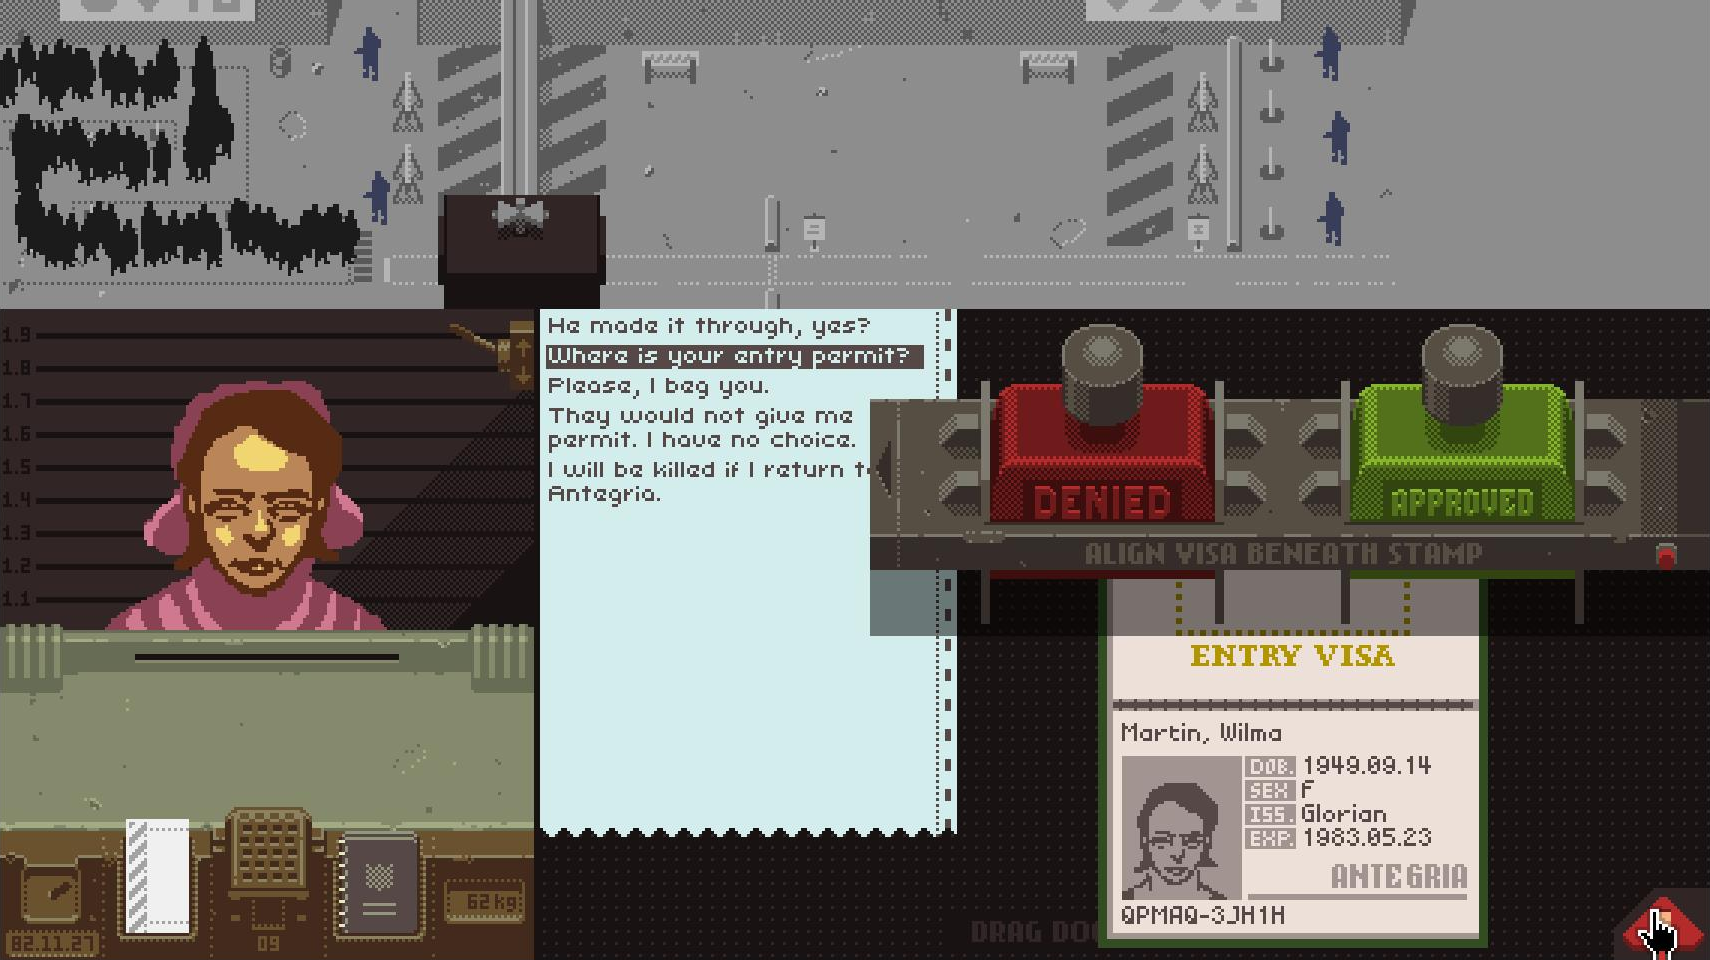
\includegraphics[width=\textwidth]{fig/papers-please-visa-choice.png}
\caption[Visa approval in \papersplease/]{A screenshot from \papersplease/ showing the interface as the player makes a decision about whether to approve or deny a visa application.}
\label{fig:visa-choice}
\end{figure}

\subsection{Analysis Example}
\label{sec:analysis-example}

To help understand the analysis technique presented here a bit better, it's useful to look at an example of its application.
%
Consider the choice shown in \cref{fig:visa-choice}, from the game \papersplease/ \citep{PapersPlease}.
%
In \papersplease/, the player takes on the role of a border security worker in charge of approving or rejecting entry applicants in a fictional dictatorship.
%
Complicating the player's role is the fact that their job is their only means of earning money to support their family, whose food, shelter, and medical needs become more pressing as the game progresses.
%
By processing applicants, the player earns credits (regardless of whether an application is approved or denied), so there is an incentive to make decisions quickly (and to avoid accepting travelers who don't meet the entry requirements, as this \emph{will} result in penalties).
%
The game focuses heavily on ethical gray areas, and the construction of its choices is central to this.
%
Although the game has various elements that go beyond explicit choices, for each applicant the player must ultimately choose to either approve or reject their visa request, and these explicit choices can be analyzed using the framework developed here.


\Cref{fig:visa-choice} shows the screen as the player is considering an entry application from a potential refugee.
%
The conversation transcript in the middle of the screen shows that this applicant claims that they will be killed if they return to their country of origin, and because of this, they seek entry despite lacking the required documents (an entry permit in this case).
%
However, the tenor of the game and the presence of applicants who will try to trick the player in various ways creates an atmosphere of suspicion, and so the player might suspect that this applicant is lying in order to gain entry.
%
As a closer analysis will show, this suspicion has interesting implications for the player's perception of this choice.

\subsubsection{Goal Analysis}

The first step of goal-based choice analysis is goal analysis, and in the absence of a real player to observe, a model player will have to suffice.
%
For the purposes of this analysis, we will assume that our model player is engaged mainly in avatar play and has the following goals (with the listed priorities):

\begin{itemize}
  \item \texttt{[high]} Provide for their family---the player wants to earn credits and avoid penalties in order to pay for food and shelter at the end of the round.
  \item \texttt{[high]} Act ethically---as much as possible, the player wants to treat applicants ethically and avoid acting in ways that would intentionally harm them without reason.
  \item \texttt{[medium]} Avoid being scammed---separate from their desire to earn credits, the player actively wants to identify dishonest applicants and deny them entry.
  \item \texttt{[low]} Admit approved travellers---in line with ethical treatment in life-or-death scenarios, the player generally wants to treat travellers fairly by letting them in if they meet the requirements for entry. This goal has a lower priority, however.
\end{itemize}

Of course not all players will have these exact goals with these exact priorities, but we can assume that many players will incorporate similar goals, and use these to develop an initial impression which can be refined further if deemed necessary.
%
In particular, an initial analysis can be modified to account for differing goal priorities or the addition or subtraction of goals, and contrasting the resulting analysis can provide further information about a choice.
%
As analysis moves forward using this list of goals, there will be opportunities to judge the results that it produces at each step and refine it if that seems necessary.

\subsubsection{Likelihood Analysis}

After analyzing goals, the next step is to analyze outcome components.
%
To simplify the analysis, we will assume that there are only two options available to the player: ``approve'' and ``deny'' (in the game, other actions are possible, but but they all either simply defer the approve/deny choice or implicitly deny the application).
%
\Cref{tab:ex-likelihoods} shows outcome components and their likelihoods for this choice; this assumes that the player is already familiar with basic gameplay in \papersplease/.
%
In particular, the player knows that if they let this traveller in, their `mistake' will not go unnoticed, and they will both fail to earn a credit and receive a punishment for their transgression (for the first mistakes of a round the punishment is merely a warning, but the player still doesn't earn credit for the mistaken approval or denial).
%
The player's doubts about the sincerity of the applicant are represented here as neutral likelihood estimates of four opposing outcomes.
%
If the applicant is telling the truth, then they are a refugee, and they are either saved by approval or condemned by denial.
%
At the same time, if they are lying, they are trying to gain entry unlawfully, and thus approving their petition has different connotations.


This is an example of how uncertain outcomes can't always be mapped directly as outcome components.
%
If ``applicant is lying'' and ``applicant is telling the truth'' were used as outcome components, these wouldn't have straightforward relationships to the player's goals, as they would be mediated by ``applicant gains entry'' and ``applicant is denied entry'' outcomes.
%
Binding the truth status of the applicant's claims together with the end result for the applicant will simplify the goal analysis step as seen in the next section.

\begin{table}[t]
\centering
\begin{tabular}{l l}
  \toprule
  \multicolumn{1}{c}{\textbf{Approve}} & \multicolumn{1}{c}{\textbf{Deny}} \\
  \midrule
  \texttt{[unlikely]} Earn a credit & \texttt{[likely]} Earn a credit \\
  \texttt{[likely]} Don't earn a credit & \texttt{[unlikely]} Don't earn a credit \\
  \texttt{[likely]} Get punished & \texttt{[unlikely]} Get punished \\
  \texttt{[unlikely]} No punishment & \texttt{[likely]} No punishment \\
  \texttt{[neutral]} Refugee is saved & \texttt{[neutral]} Refugee is saved \\
  \texttt{[neutral]} Refugee is condemned & \texttt{[neutral]} Refugee is condemned \\
  \texttt{[neutral]} Scam is rewarded & \texttt{[neutral]} Scam is rewarded \\
  \texttt{[neutral]} Scam is thwarted & \texttt{[neutral]} Scam is thwarted \\
  \bottomrule
\end{tabular}
\caption[Example likelihood analysis]{Likelihood analysis for the example choice shown in \cref{fig:visa-choice}.}
\label{tab:ex-likelihoods}
\end{table}


\subsubsection{Option Analysis}

Given the provide-for-family, act-ethically, avoid-scams, and admit-approved goals identified during goal analysis and the outcome components from likelihood analysis, the next step of goal-based choice analysis is to combine this information in an assessment of each option's perceived relationship to each player goal.
%
\Cref{tab:ex-option-analysis} shows the results, using the \lbl{enables}, \lbl{threatens}, \lbl{advances}, and \lbl{hinders} labels described in \cref{sec:cp-option-analysis}.
%
Note that the provide-for-family goal exhibits a strong distinction between the two cases, based on the \lbl{likely} and \lbl{unlikely} credit and punishment outcome components.
%
In contrast, the act-ethically and avoid-scams goals have only weak expectations, because the associated outcome components are uncertain.
%
The admit-approved goal is irrelevant here, because the applicant in question is not an approved traveller.


The assignments in \cref{tab:ex-option-analysis} are based on individual outcome-component/goal relationships: the credit- and credit-related outcome components are relevant to the provide-for-family goal, while the other four outcome components relate to the act-ethically and avoid-scams goals.
%
As stated above, the breakdown of outcome components was chosen so that their relationships to player goals would be straightforward.
%
This allows the likelihood labels to capture any uncertainty in the situation, as opposed to having unclear or conditional relationships between outcome components and goals.

\begin{table}[b]
\centering
\begin{tabular}{c l l}
  \toprule
  \textbf{Goal} & \multicolumn{1}{c}{\textbf{Approve}} & \multicolumn{1}{c}{\textbf{Deny}} \\
  \midrule
  \multirow{2}{9em}{\centering provide-for-family} & \lbl{threatens} & \lbl{enables} \\
                                        & \lbl{hinders} & \lbl{advances} \\
  \midrule
  \multirow{2}{9em}{\centering act-ethically} & \lbl{enables} & \lbl{enables} \\
                                 &               & \lbl{threatens} \\
  \midrule
  \multirow{2}{9em}{\centering avoid-scams} & \lbl{enables} & \lbl{enables} \\
                                 & \lbl{threatens} & \lbl{threatens} \\
  \midrule
  admit-approved & $<$none$>$ & $<$none$>$ \\
  \bottomrule
\end{tabular}
\caption[Example option analysis]{Option analysis for the example choice shown in \cref{fig:visa-choice}.}
\label{tab:ex-option-analysis}
\end{table}

\subsubsection{Relative Option Analysis}

The relative option analysis step looks for patterns in the results of option analysis, but in this case, the option analysis doesn't fit any established patterns.
%
In this case, known patterns can still be used as guideposts if we can figure out a known pattern that almost fits and analyze why it doesn't.
%
For this particular choice, it turns out that the \lbl{dilemma} pattern is a near match if the option analysis is a bit different.


In fact, the player's doubt of the applicant's story is key here.
%
\Cref{tab:ex-revised-option-analysis} shows an alternative option analysis if the player assumes that the applicant is telling the truth.
%
Such an alternate assumption changes the likelihood analysis (not shown), making the refugee-related outcomes \lbl{likely}/\lbl{unlikely}, and the scam-related outcomes universally \lbl{unlikely}.
%
The results for the option analysis in \cref{tab:ex-revised-option-analysis} show that the \lbl{advances}/\lbl{hinders} dichotomy of the provide-for-family goal is now reversed at the act-ethically goal.
%
The resulting pairing of opposed \lbl{hinders} labels almost meets the requirements for the \lbl{dilemma} pattern, except that it also includes \lbl{enables}/\lbl{advances} assignments.
%
In fact, the \lbl{dilemma} pattern criteria in \cref{tab:prospective-impressions} is specific to a \emph{classic} dilemma where neither option has redeeming qualities, but in this case we have a dilemma where the choice is between two conflicting goals and in either case the one that isn't \lbl{hindered} will be \lbl{advanced}.


Despite the caveats, we can see that if the player trusts the applicant they face a kind of dilemma.
%
This means that the original choice is like a dilemma, except for the issue of doubt: if the player trusts the applicant, they face an ethical quandary---a decision between feeding their family and sheltering a refugee.
%
However, if the player begins to doubt the applicant, the results of option analysis indicate that denying the application is clearly superior to approving it: denying the application \lbl{advances} a high-priority goal that approving it would \lbl{hinder}, and no other high-priority goals include such a clear distinction in terms of expected outcomes.


Looking at this result, we can see a broader message that \papersplease/ is trying to convey.
%
In this choice and others through the game, would-be ethical dilemmas are tilted by doubt, and the overall formula becomes ``dilemma $+$ doubt $\rightarrow$ complicity''---by introducing doubt about the people who want to cross the border, while making the risk/reward situation clear with respect to the player's prospects for feeding their family, the player's choices are tilted towards complicity with the regime's calculating but ultimately inhumane priorities.
%
The callous response---leaving the potential refugee to their fate---becomes the rational one, and every would-be smuggler further justifies these decisions.
%
Through its choice structures, \papersplease/ is showing the player what it feels like to be in this kind of situation and thus demonstrating why someone in that situation might make a particular set of decisions.
%
The poetics of its choices, particularly when they give rise to feelings of moral uncertainty or doubt of the applicants, are an important part of this.


\begin{table}[!t]
\centering
\begin{tabular}{c l l}
  \toprule
  \textbf{Goal} & \multicolumn{1}{c}{\textbf{Approve}} & \multicolumn{1}{c}{\textbf{Deny}} \\
  \midrule
  \multirow{2}{9em}{\centering provide-for-family} & \lbl{threatens} & \lbl{enables} \\
                                        & \lbl{hinders} & \lbl{advances} \\
  \midrule
  \multirow{2}{9em}{\centering act-ethically} & \lbl{enables}  & \lbl{threatens} \\
                                              & \lbl{advances} & \lbl{hinders} \\
  \midrule
  avoid-scams & $<$none$>$ & $<$none$>$ \\
  \midrule
  admit-approved & $<$none$>$ & $<$none$>$ \\
  \bottomrule
\end{tabular}
\caption[Example option analysis]{An alternate option analysis for the example choice shown in \cref{fig:visa-choice}. This analysis assumes that the applicant is telling the truth about their situation (compare this table to \cref{tab:ex-option-analysis}).}
\label{tab:ex-revised-option-analysis}
\end{table}

\subsubsection{Outcome Component Analysis}

Although the prospective analysis of our example choice has revealed something interesting about its structure, analyzing how the actual results are perceived is also important.
%
For outcome component analysis, each \emph{actual} outcome component should be analyzed with respect to each player goal.
%
If desired, this can focus only on the outcome components of a single option to understand what players who choose that option will feel.


Focusing then on the option to \emph{approve} the applicant's petition for entry, what are the actual outcome components?
%
In \papersplease/, whenever someone is let through who does not meet the technical requirements for entry the player accrues a citation, the first two of which in a given round result in warnings with the third and subsequent citations resulting in a fine equal to the amount of credits earned for processing one applicant.
%
At the same time, letting in someone who should not be admitted does not earn credit towards one's salary (although interestingly, denying someone who deserves entry does, even when a citation is issued for an erroneous denial).
%
In this specific case, even assuming that the player has not made any mistakes in the current round, a warning means that future mistakes are more risky, so accruing one has a minor negative effect on the player's provide-for-family goal.
%
At the same time, the no-credit-earned outcome of an approval has a major negative impact on the player's provide-for-family goal: a denial would have earned credit for the time spent considering the application, and time is a very limited resource in the game.


Although these two outcome components (the citation and lack of credit) are straightforward, what about the outcome components related to either saving a refugee or catching a scammer?
%
In \papersplease/, after approving entry, one does not magically get to know whether the applicant was honest or not.
%
In other words, even once a decision is made in this case, the player still doesn't find out whether they were justified or not.
%
These outcome components remain uncertain: the applicant was let in, but was that a good thing or not?
%
The player can only rely on their judgement of the sincerity of the applicant's claims in this case.


Although goal-based choice analysis has no explicit suggestions as to how to handle this case of post-decision lingering uncertainty (perhaps this could be a direction for future work), we can think about what impact this might have in this specific case.
%
For the outcome component analysis step, we will just analyze both components separately and keep in mind that the player doesn't know which of them occurs.
%
This results in the outcome component judgements shown in \cref{tab:ex-outcome-component-analysis}.

\begin{table}[!b]
\centering
\begin{tabular}{>{\centering}m{6em} >{\centering}m{6em} >{\centering}m{6em} >{\centering}m{6em} >{\centering}m{6em}}
  \toprule
  & \textbf{no-credit-earned} & \textbf{citation-issued} & \cg{\textbf{refugee-sheltered*}} & \cg{\textbf{scam-rewarded*}} \tabularnewline
  \midrule
  \textbf{provide-for-family} & major \\ negative & minor \\ negative &  &  \tabularnewline
  \midrule
  \textbf{act-ethically} &  &  & \cg{major \\ positive} &  \tabularnewline
  \midrule
  \textbf{avoid-scams} &  &  &  & \cg{major \\ negative} \tabularnewline
  \midrule
  \textbf{admit-approved} &  &  &  &  \tabularnewline
  \bottomrule
\end{tabular}
\caption[Example outcome component analysis]{Outcome component analysis for the \emph{approve} option at the example choice shown in \cref{fig:visa-choice}. Each entry lists the impact of an outcome component on a goal. The outcome components marked with asterisks are opposing potential components that the player is uncertain of even after making a decision.}
\label{tab:ex-outcome-component-analysis}
\end{table}


Recall that our choice of outcome components made the option analysis step simple; in this case that has in turn made the outcome component analysis step complex.
%
Because this choice has an inherently complicated structure due to the hypothetical player's unresolved doubts about the applicant's honesty, it is not simple to represent in terms of outcome components with direct relationships to player goals, but breaking it down into outcome components is still useful in order to identify where the complexity resides.
%
An alternate analysis would simply use ``applicant admitted'' as an outcome component, and label its goal-impacts on both the act-ethically and avoid-scams goals as uncertain.
%
The breakdown used here instead provides more detail by showing the evaluations corresponding to each potential player belief (in other words, by showing what possibilities the player is uncertain about).

\subsubsection{Full Outcome Analysis}

Based on the results of outcome component analysis, full outcome analysis summarizes each option as being overall good/bad and expected/unexpected/unpredictable with respect to player goals.
%
Focusing again only on the approve option, we can see that its outcome is mixed but mostly negative.
%
It has definite negative impacts on the high-priority goal of providing for the player's family, but it also has an uncertain positive impact on the high-priority goal of treating applicants ethically.
%
Even if the uncertain impact on the avoid-scams goal is ignored because that goal has a lower priority than the two just mentioned, the positive impact on the act-ethically goal is less certain than the negative impacts on the provide-for-family goal, and so the overall impact can be summarized as a \lbl{tradeoff} with both good and bad components which leans towards the negative.


In terms of predictability, there's nothing surprising about this outcome (all of the \emph{actual} outcome components were \emph{expected}) so it falls into the \lbl{expected} corner, although we have to keep in mind the persistent uncertainty about whether the applicant was being truthful or not, which adds an element similar to unpredictability.
%
As a whole then, the ``approve'' option is an expected tradeoff which leans negative, and which comes with a lingering uncertainty about its actual outcomes.
%
The ``deny'' option sustains a mirrored analysis (omitted here for brevity), and appears as an expected tradeoff which leans positive, again with some uncertainty over actual outcomes.


Note that the psychological implications of these outcomes are interesting given the human tendency to rationalize one's decisions (see e.g., \citep{Hall2012}).
%
One might expect players who chose to approve this applicant's entry to believe more strongly after-the-fact that the applicant was telling the truth, and vice versa for those who chose to deny entry.
%
This is one mechanism by which \emph{making a decision} can actually influence players' perceptions of the structure of a choice.
%
This is also a mechanism which reinforces complicit behavior as mentioned above, and \papersplease/ is intentionally creating these choice structures in order to force the player to experience exactly this kind of fraught decision-making.


\subsubsection{Retrospective Analysis}

Having analyzed each outcome as a unit, the final step in goal-based choice analysis is to try to understand a particular choice in terms of existing choice-structure patterns.
%
In this case, none of the retrospective impression labels in \cref{tab:retrospective-impressions} apply to either option at this choice, because they are all aimed at clearly-good or -bad outcomes, and the outcomes of both options here are tradeoffs which involve additional uncertainty.
%
Even without matching against a known structure however, the breakdown of outcome evaluations has already been informative.


As mentioned above, \papersplease/'s illustrates how uncertainty can lead to complicity when ethically-questionable decisions are seen as having uncertain results on one side and guaranteed results on another.
%
In order for this to be clear, the player must experience both moral doubt and uncertainty, and these feelings arise from the structure of choices such as the one analyzed here.
%
The uncertainty that the player experiences can be seen as having two parts which have been identified by this analysis: before making a decision, the player is uncertain about the applicant's honesty, and afterwards, this translates to uncertainty about the true outcome of their decision.


The player's initial uncertainty is due to a pattern of options and outcomes established across many choices by the game.
%
As the player plays, they face many applicants who attempt to lie or bluff their way past the checkpoint despite having suspicious documents.
%
Other events, such as a terrorist attack on the checkpoint, set a grim mood, and this pattern of events serves to make the player generally suspicious (the interface and basic interaction loop of identifying and questioning discrepancies also contribute).
%
Altogether, this suspicion leads the player to question the moral character of applicants in general, and in the specific choice discussed here this results in an uncertain likelihood analysis which views the applicant's refugee status as an unknown variable.


This suspicion-of-the-applicant then translates to a questioning of the player's decision once it has been made.
%
Whether the player approves or denies the applicant's entry petition, concrete results (in terms of earning or not earning credits to help support their family) are contrasted with lingering doubts about whether the applicant deserved entry or not.
%
\papersplease/ intentional leaves the true outcomes of the player's actions ambiguous with respect to their goals, creating lingering doubt which builds as the player continues to make questionable decisions.
%
This creates a situation where the player can come to doubt their own judgements and second-guess themselves, which adds a second layer of uncertainty.
%
Especially when confronted with similar choice structures repeatedly throughout the game, this second-guessing can help push the player to confront their decisions and thereby think about what message the game is trying to convey in this regard.


In this case, even though the elements of choice structure identified did not fit the pattern of any already-identified retrospective impression, identifying elements such as uncertainty and moral ambiguity was enough to gain insight into how this choice functions within \papersplease/.
%
Breaking things down also allows us to understand why the choice produces the effects that it does, and which specific elements of the choice are necessary for it to function as intended.
%
For example, the analysis presented here makes it clear that this choice functions as it does because it brings two ethical imperatives into conflict (supporting those who depend on you and avoiding harm to innocents) but then has uncertain outcomes in terms of one of them (avoiding harm).
%
Altering one of these elements (for example, making it so that earning credits is random, and thus the reward in terms of supporting one's family is also ambiguous) would change the character of this choice.


\section{Overview \& Future Work}

As just demonstrated, goal-based choice analysis breaks down a choice into individual options and components, analyzes them with respect to a specific set of player goals, and by doing so helps present a clear picture of how the structure of a choice contributes to its poetic function\footnote{As demonstrated such analysis may also be useful for understanding a choice's rhetorical and/or hermeneutic functions.} within a work.
%
The analysis method presented here is heavily dependent on identifying well-understood prospective and retrospective impressions and good criteria for their application.
%
However, this chapter only presents a few of these impressions, and it does not contain a comprehensive analysis of the poetic effects that they can create.
%
In other words, the theory of choice poetics described here is still preliminary.
%
However, this goal-based choice analysis is a strong framework for understanding nuanced choices, because decomposing options and outcome components can help untangle complex choice structures.
%
Additionally, by separating player goal analysis from the main choice analysis and taking modes of engagement into account, this method makes the dependencies between desired impressions and particular player goals visible to designers.
%
Without such visibility, the confusion of players faced by a choice that pits two modes of engagement against each other might be mysterious to a designer who favors one of the modes and doesn't realize that the other is relevant.
%
Goal-based choice analysis could thus be helpful for debugging key choice structures that aren't producing a desired impression, and for figuring out whether a game supports specific modes of engagement.


The few impressions that have been presented here have also been verified to some degree by the experiments presented in \cref{ch:option-results,ch:outcome-results}.
%
In fact, the results of those experiments did not unanimously confirm my hypotheses, which has led to refinements in the analysis technique presented here.
%
In particular, \cref{tab:prospective-impressions,tab:retrospective-impressions} are revisited in \cref{tab:prospective-impressions-redux,tab:retrospective-impressions-redux} in \cref{sec:results-prospective-caveats}.
%
These revisions and others that were made as I built \dunyazad/ are the primary product of my hybrid research method: a more nuanced understanding of choice poetics obtained by attempting to operationalize it.


One might wonder what advantage this analysis technique has over similar theories that could be applied to narrative choices, such as decision affect theory \citep{Mellers1997} (which it is in part based on).
%
One difference lies in specificity and directness: while decision affect theory could be consulted to come up with a set of hypotheses about audience response to a choice, it does not provide a list of specific steps to follow in doing so.
%
Another difference is the aims of the theories: decision affect theory has been shown to have explanatory and predictive power: it can be used to explain observed reactions to choices, and it can be used to predict reactions given a choice.
%
In contrast, goal-based choice analysis as presented here was designed to have \emph{generative} power: it can be used to \emph{construct} a choice that produces a specific reaction.
%
Although further studies could hopefully demonstrate that goal-based choice analysis has explanatory and predictive power as well, the results presented in \cref{ch:option-results,ch:outcome-results} are a validation of generative power.
%
Of course, if one is interested in generating rather than evaluating choices, this evidence is encouraging.


The next step in developing goal-based choice analysis would be to greatly expand the number of prospective and retrospective impressions scrutinized.
%
An efficient approach would be to take a well-known interactive experience built around explicit discrete narrative choices and analyze it from the beginning, breaking down each choice within this framework and looking for patterns in their usage.
%
\dunyazad/ could then be used to double-check and refine the insights generated by this process: take each impression identified during the initial analysis, encode it in \dunyazad/, and ask \dunyazad/ to generate choices that involve that impression.
%
Some of the choices generated will likely not appear to give that impression upon initial inspection, and \dunyazad/'s full output can be used to figure out exactly how the criteria that were developed technically fit the generated choice.
%
With this information, refinements to \dunyazad/ and/or the underlying theory can be made, eventually producing both an analytical and a generative model of the impression in question, and completing the analysis $\rightarrow$ theory $\rightarrow$ generative model $\rightarrow$ experimentation cycle.


The next chapter describes in detail how \dunyazad/ operates, and part of it mirrors this one: an automated version of the analysis technique described here forms the core of \dunyazad/'s reasoning capabilities.
%
After that, \cref{ch:option-results,ch:outcome-results} discuss the results of two experiments that showed outputs from \dunyazad/ to humans and gathered feedback about their impressions.
%
\Cref{ch:outcome-results} includes some updates to the material presented here (mainly \cref{tab:prospective-impressions,tab:retrospective-impressions}; see \cref{sec:results-prospective-caveats}), as these refinements make the most sense when presented alongside the experimental results that led to them.

\chapter{\dunyazad/}

\label{ch:dunyazad}%

As stated in the introduction, \dunyazad/ has two purposes as a project: first, to produce a \emph{system}, and second, to produce a \emph{theory}.
%
The system is a novel story generator that is focused on generating interesting choices, and on providing fine-grained control over the kinds of choices it uses.
%
The theory is a theory of choice poetics: a theory about how specific choice structures give rise to certain feelings, such as regret.
%
In order to satisfy these two goals, \dunyazad/ uses an answer set solver to turn a logical criteria for a certain kind of choice into an instance of such a choice---this is its core operating principle.


\dunyazad/'s code therefore largely consists of a set of logical statements describing what a choice structure is and when choices fit into one of several categories.
%
For example, there are statements that define a ``relaxed'' choice.
%
Answer sets that satisfy these constraints are found using Potassco Labs' \clingo/ solver \citep{Gebser2011}.
%
Besides these rules, there is an external control structure which invokes the solver repeatedly, generating multiple choices and connecting them into a story.\footnote{
The model for \dunyazad/'s output is the Choose-Your-Own-Adventure book.
%
These books are young-adult novels which contain explicit choices: at the end of certain pages, the reader is instructed to choose an action for the protagonist, and continue reading at one of several different pages depending on their choice.
%
This combination of traditional linear narrative with intermittent discrete choices is one of the most straightforward examples of what I call ``choice-based narrative.''
%
Note that in contrast to Choose-Your-Own-Adventure books, choices in \dunyazad/ are separated by only a few sentences, rather than pages of text.}
%
The focus of development so far has been on individual choices, but the capacity exists for \dunyazad/ to generate a full branching story.
%
Of course, there is also some imperative code for turning a logical choice structure into English text, in the form of a template-based generation system.
%
The English-generation code and the control code are both written in Python.


The goal of this chapter is to describe in detail how \dunyazad/ functions.
%
First, \cref{sec:dunyazad-asp-and-ctp} describes why \dunyazad/ uses answer set programming in a bit more detail, and how answer set programming (ASP) helps with the theory development goal.
%
\Cref{sec:dunyazad-choice-generation} then describes how \dunyazad/ generates individual choices, while \cref{sec:dunyazad-control} describes the higher-level control mechanism.
%
Finally, \cref{sec:dunyazad-summary} summarizes the entire system and works through an example of how \dunyazad/ generates a choice from beginning to end.
%
Note that the template-based English generation system is described separately in \cref{ap:nlg}.

%\section{Goals}

\section{ASP and Critical Technical Practice}
\label{sec:dunyazad-asp-and-ctp}%

The idea of critical technical practice started as a call for technical practitioners (and especially AI researchers) to be more aware of the limits placed on their technical approaches by the central metaphors of their fields.
%
In Phil Agre's 1997 \work{Computation and Human Experience} he describes a process of critical examination to identify core metaphors and what those core metaphors marginalize, followed by an inversion that makes those marginalized concepts central \citep{Agre1997}.
%
This process can be used to drive innovation and find hidden limitations in a technical field by scrutinizing it using the tools of critical theory.


One common AI practice identifies a motivating theory from another discipline and then attempts to build a system that faithfully operationalizes that theory, taking the theory for granted as a known truth.
%
In contrast, critical technical practice seeks to question common assumptions (in particular through the application of critical theory) and then embark upon technical projects that use non-standard assumptions, thereby broadening the technical field.
%
\dunyazad/ as a project pursues a different relationship between theory and practice by seeing its driving theory (choice poetics) as both a \emph{product} of technical practice and a precursor to it, integrating theory development tightly with system development so that both the theory and the system are developed in dialogue with each other.
%
\dunyazad/ thus questions its theoretical assumptions as a matter of course and in fact uses difficulties encountered during technical development to prompt changes in the theory of choice poetics.
%
In fact, \dunyazad/ can be seen as using artificial intelligence as a tool of criticism in the refinement of a theory, just as much as it uses theory to guide the development of an artificial intelligence.


In order to jointly develop \dunyazad/ as a system and choice poetics as a theory, a special technical approach is required---this is where answer set programming comes in.
%
One could imagine choice-point generators constructed using many different technologies, from case-based reasoning to something as complicated as neural networks.
%
However, most of these would fail to achieve the level of \emph{transparency} required for the system to provide useful feedback to the underlying theory.
%
In a neural-network based approach, for example, it would be very difficult to understand which part of the underlying theory is responsible for a particular generated choice structure, and even more difficult to use experimental results to inform changes in the theory.
%
Answer-set programming as a technical approach is thus motivated by the goal of developing choice poetics alongside a technical system for generating choices.


The reason that answer-set programming is useful for critical technical practice is that answer set programs consist of a series of logical statements which dictate which combinations of predicates are allowed in the output.
%
This means that every predicate in the output set can be traced back to a set of rules in the program which allowed it to be present.
%
Sometimes this process is laborious, as many rules may chain together to allow a predicate, but  ultimately, every aspect of an answer-set program's output can be analyzed to figure out which specific statements were responsible for its presence.
%
Furthermore, because those logical statements correspond directly to elements of the underlying theory, the relationship between that theory and the program's output is visible.


As an example, \dunyazad/ has rules that define one way in which a choice can be obvious---by having exactly one option which suggests a positive outcome and one or more options all of which suggest negative outcomes.
%
Originally, the criterion that the other options must suggest negative outcomes was not present, but upon looking at generated choices, some clearly didn't fit an intuitive test for obviousness because of their inclusion of neutral options.
%
Identifying the inclusion of these neutral options as the problem was easy, and it was also clear from inspection of the code that without a clause in the definition of ``obvious'' prohibiting neutral options, they would be allowed.
%
The fix at the system level was the extra clause requiring that all options at an obvious choice except the ``correct'' option should suggest negative outcomes.
%
Of course, this was not only a change in the code, it was also a change in the theory, because \dunyazad/'s code is a direct operationalization of choice poetics.
%
Obvious choices don't just have ``only one good option,'' instead they have ``one option which stands out from the rest as significantly better.''


In contrast with many techniques that could be applied to the problem of generating choice points, answer-set programming uniquely enables a tight integration of system development with theory development.
%
The use of answer-set programming as a design choice is thus driven not only by considerations at the system level, but also at the project level: in order for \dunyazad/ to produce both a system and a theory, the use of answer-set programming is critical.
%
In \dunyazad/, answer-set programming helps support the aims of critical technical practice by helping make the system's underlying assumptions clearly visible, and by making every change to the system suggest a parallel change to the theory that it implements.

% TODO: Use this mini-rant somewhere?
%In contrast, statistical techniques often hide such assumptions through their use of data which is assumed to be unbiased and universally representative.
%
%In fact, the data sets used to drive statistical artificial intelligence techniques often contain many assumptions, but examination of these is far from straightforward and is seen a peripheral to most technical projects if it is considered at all.


\section{Choice Generation}
\label{sec:dunyazad-choice-generation}%

\dunyazad/ generates choices by solving complicated logic problems.
%
These problems are set up so that any solution will take the form of a choice, and further constraints can dictate certain properties of that choice (for example, that it must be an obvious choice).
%
Broadly, \dunyazad/'s constraints can be split into four categories:

\begin{itemize}
\item \textbf{Representational constraints} establish the basic elements that \dunyazad/ arranges to form choices and stories.
\item \textbf{Constituent constraints} define the most basic rules for configuring representative elements to construct choices and stories.
\item \textbf{Aesthetic constraints} carve out a region within the space allowed by the constituent constraints, excluding gibberish and other categorically undesirable configurations.
\item \textbf{Poetic constraints} make distinctions between different desirable configurations and are selectively activated to produce different kinds of choices.
\end{itemize}

To understand how \dunyazad/ functions, it is first necessary to understand \dunyazad/'s (rather limited) view of what a choice is, and how choices fit together to form stories.
%
These things are defined by representational and constituent constraints.


\subsection{Story Representation}


In \dunyazad/, a story is represented as a sequence of actions, each drawn from a pre-determined set.
%
Besides actions, each timepoint in a story has an initial state, which can include characters, items, and relations between them.
%
\dunyazad/ also has ``setups,'' which are used to establish interesting situations that motivate action.
%
This kind of representation is amenable to logical reasoning and similar to representations used in planning-based story generation systems.
%
It is sufficient to represent a wide variety of simple stories focused on action (as opposed to say, character growth or the development of relationships).
%
Luckily, many of the original Choose-Your-Own-Adventure books are focused on actions and consequences, and the format of choice-based narrative lends itself to such stories, because they give rise to interesting choices.


\subsubsection{States}

\dunyazad/'s representational constraints define predicates for ``instances,'' which may be either ``actors'' or ``items,'' as well as ``states'' (binary properties of an instance), ``properties'' (instance properties which can be multi-valued), and ``relations,'' (named directional instance-to-instance links).
%
Besides these things, which can change from one state to the next as a result of the outcomes of actions, instances can have timeless ``surface properties'' like a name, which is stored but cannot be changed by events in the story.
%
\Cref{fig:dunyazad-states} gives examples of each of these and \cref{fig:dunyazad-state-example} shows how they come together to describe a situation.


\begin{figure}[!t]
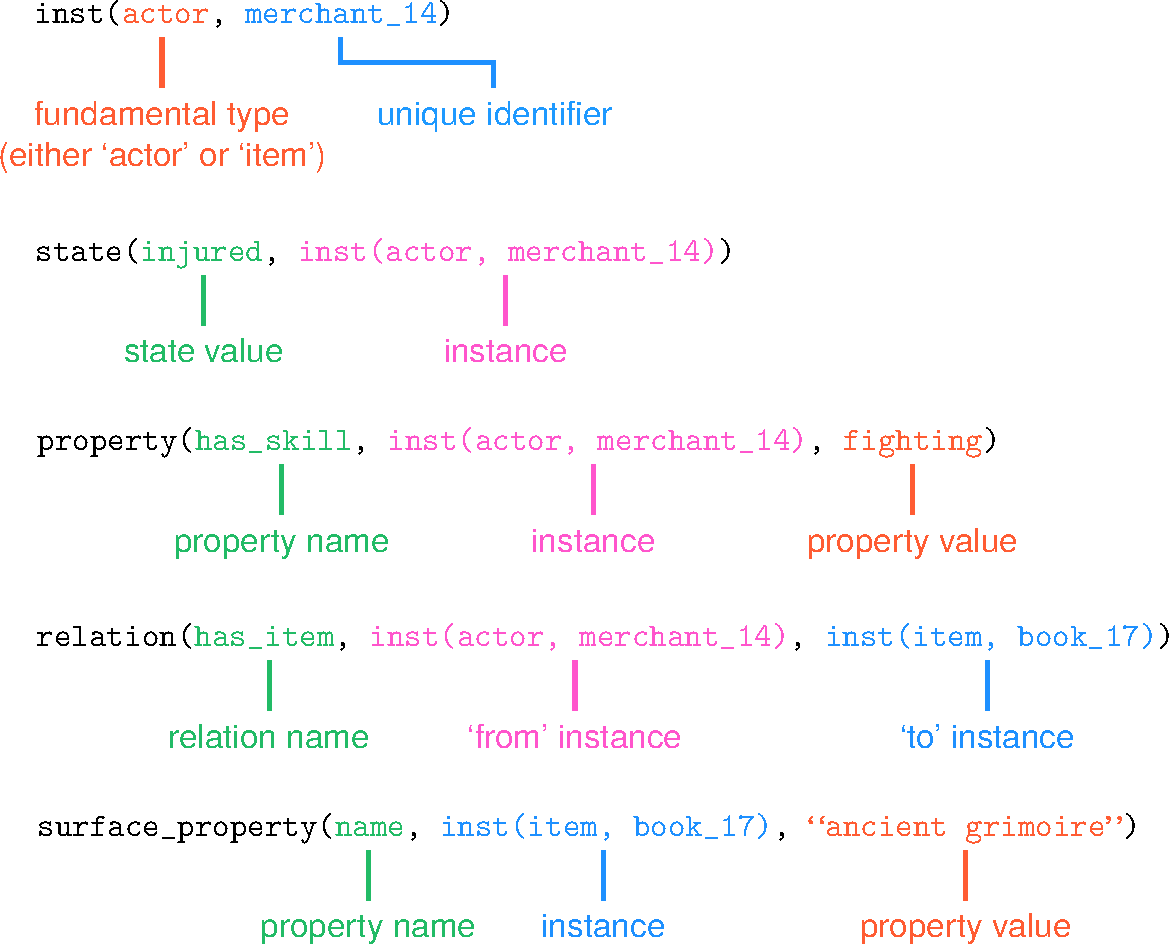
\includegraphics[width=\textwidth]{fig/cropped-dunyazad-states.pdf}
\caption[\dunyazad/'s state predicates]{Predicates used to describe states in \dunyazad/.}
\label{fig:dunyazad-states}
\end{figure}


The core states in \dunyazad/ describe the cast and any items or skills that those characters possess.
%
Beyond these states are a group of states that describe transient relationships that set the stage for action; these are called ``potentials.''
%
Potentials include things like \prq{knows\_gossip}{,} \prq{injured}{,} and \prq{threatening}{,} and each is classified as either a ``problem'' or an ``opportunity.''
%
Although these special potential states are represented using normal \prq{state}{,} \prq{property}{,} and \prq{relation}{} predicates, actions which get rid of them must specify whether each potential is \prq{resolved}{,} \prq{manifested}{,} or \prq{nullified}{.}
%
Additionally, extra predicates specify whether a potential is \prq{problematic\_for}{} one or more of the actors involved (for example, the \prq{injured}{} state is \prq{problematic\_for}{} any actor to which it is applied).


\dunyazad/ understands based on this information whether the action which eliminated a potential was good or bad for different characters.
%
For example, an action that \prq{resolves}{} an \prq{injured}{} state is good for the actor who was injured, and thus taking that action makes sense for that character.
%
States themselves thus directly encode some of the information used to decide which actions are viable.
%
This not only helps the system reason about motivation, but it also makes the design of actions and setups easier by providing a standard set of states that trigger certain actions.


\begin{figure}[!b]
\centering
\fbox{%
\parbox{0.9\textwidth}{
Scene:\svind\\
\ind \parbox{0.95\linewidth}{\quoteshape A merchant carrying some perfume is being threatened by bandits.}\vind\\
Representation:\svind \\
\ind \parbox{0.9\textwidth}{ \tt
inst(actor,businessperson\_4). \\
inst(actor,tough\_3). \\
inst(item,treasure\_5). \\
property(type,inst(actor,businessperson\_4),merchant). \\
property(type,inst(actor,tough\_3),bandits). \\
property(type,inst(item,treasure\_5),perfume). \\
relation( \\
\ind has\_item, \\
\ind inst(actor,businessperson\_4), \\
\ind inst(item,treasure\_5) \\
). \\
relation( \\
\ind threatening, \\
\ind inst(actor,tough\_3), \\
\ind inst(actor,businessperson\_4) \\
). \\
surface\_property(name,inst(item,treasure\_5),"perfume").
}
}
}
\caption[\dunyazad/ state example]{An example scene description using \dunyazad/'s internal representation, showing the most-relevant predicates. In real output, each of these predicates except the \prq{surface\_property}{} would be tied to a specific timepoint, and there would be many more \prq{surface\_property}{} predicates describing things like the name of each instance and whether it is plural or singular. Note that each instance is assigned a unique identifier that ends with a number.}
\label{fig:dunyazad-state-example}
\end{figure}


\Cref{fig:dunyazad-state-example} is not quite accurate, because \dunyazad/'s non-surface state predicates are never encountered raw.
%
Instead, they are wrapped in \prq{st(<timepoint>, <state>)}{} predicates, to define different states of the world for each timepoint in the story.
%
The timepoints in a story form a directed acyclic graph that branches out from a single root node.
%
The structure of this graph is defined using \prq{successor(<previous>, <option>, <next>)}{} predicates which specify that the result of choosing option \prq{<opt>}{} at timepoint \prq{<previous>}{} is the state designated \prq{<next>}{.}
%
The root timepoint is named \prq{root}{,} and each successor is named for its parent plus the number of the option that leads to it, so for example, if there were three options at the \prq{root\_2}{} node, they would lead to timepoints labelled \prq{root\_2\_1}{,} \prq{root\_2\_2}{,} and \prq{root\_2\_3}{.}
%
The timepoints do not necessarily form a tree, however: if two outcomes lead to identical states, as long as it would not form a cycle in the graph, \dunyazad/ may connect them to the same timepoint.


\subsubsection{Actions}

As mentioned above, timepoints in \dunyazad/ are connected by options.
%
Each option is associated with a single action, and arguments describe the details of that action (for example, who initiated it or who the target is).
%
If a timepoint has more than one option, it represents a choice to be made by the player, otherwise it is simply an event that happens.
%
Actions specify lists of outcome variables with values for each variable.
%
For each outcome variable that an action has, a single outcome value is assigned to each option that uses that action, thereby defining the entire impact of that option on the world state.
%
These assignments have a shorthand notation \prq{o(<variable>, <value>)}{} which indicates that the outcome variable \prq{<variable>}{} takes on the value \prq{<value>}{.}
%
Each such assignment is an outcome component, and together, all such assignments for an action are the outcome of that action.
%
\Cref{fig:dunyazad-action-example} shows an example where at timepoint \prq{root}{,} the action associated with option 1 is \prq{talk\_down}{,} with two outcomes: \prq{o(attitude, convinced)}{} and \prq{o(is\_enraged, not\_enraged)}{}.
%
Note that each outcome variable is responsible for deciding whether or not a particular state change occurs (or between several possible state changes one of which must occur).
%
The consequences of an action in terms of the world state are thus fully determined by the values of its outcome variables.

\begin{figure}[!t]
\centering
\fbox{%
\parbox{0.9\textwidth}{
Option:\svind\\
\ind \parbox{0.95\linewidth}{\quoteshape You try to talk the bandits down.}\vind \\
Outcome:\svind\\
\ind \parbox{0.95\linewidth}{\quoteshape You talk to the bandits and convince them to back off.}\vind \\
Representation:\svind \\
\ind \parbox{0.9\textwidth}{ \tt
\cg{at(root,} action(option(1), talk\_down)\cg{).} \\

\cg{at(root,} arg(option(1), asking, inst(actor, you))\cg{).} \\
\cg{at(root,} arg(option(1), listening, inst(actor, tough\_3))\cg{).} \\
\cg{at(root,} arg(option(1), victim, \\
\ind inst(actor, businessperson\_4))\cg{).} \\

\cg{at(root,} outcome(option(1), o(attitude, convinced))\cg{).} \\
\cg{at(root,} outcome(option(1), o(is\_enraged, not\_enraged))\cg{).} \\

\cg{at(root,} consequence\_of(option(1), o(attitude, convinced), \\
\ind \_not, relation(threatening, \\
\ind \ind inst(actor, tough\_3), inst(actor, businessperson\_4)))\cg{).} \\
\cg{at(root,} consequence\_of(option(1), o(is\_enraged, enraged), \\
\ind relation(threatening, \\
\ind \ind inst(actor, tough\_3), inst(actor, you)))\cg{).} \\

\cg{at(root,} consequence(option(1), \\
\ind \_not, relation(threatening, \\
\ind \ind inst(actor, tough\_3), inst(actor, businessperson\_4)))\cg{).}
}
}
}
\caption[\dunyazad/ action example]{An example of action representation in \dunyazad/. Note that even outcomes which do not occur (\prq{o(is\_enraged, enraged)}{} in this case) have their potential consequences noted via \prq{consequence\_of}{} predicates (so that the system can reason about counterfactuals), but only outcomes that do occur (as specified by the \prq{at(<timepoint>, outcome(option(<opt>), o(<outvar>, <outval>)))}{} predicates) have actual consequences. The \prq{o(attitude, unconvinced)}{} and \prq{o(is\_enraged, not\_enraged)}{} possible outcome components are not listed because they make no changes to the world state when they occur (they each represent the omission of a change).}
\label{fig:dunyazad-action-example}
\end{figure}


Each action thus has multiple possible outcomes.
%
For the \prq{talk\_down}{} action, there are theoretically four: the \prq{attitude}{} outcome variable has two exclusive values \prq{convinced}{} and \prq{unconvinced}{,} while the \prq{is\_enraged}{} outcome variable has two more values: \prq{enraged}{} and \prq{not\_enraged}{.}
%
However, the definition of \prq{talk\_down}{} stipulates that the outcome \prq{o(is\_enraged, enraged)}{} is only possible if the outcome \prq{o(attitude, unconvinced)}{} is also present, so there are only three possibilities:

\begin{enumerate}
  \item The target is convinced to calm down (\prq{o(attitude, convinced)}{} and \prq{o(is\_enraged, not\_enraged)}{}), in which case they stop threatening whoever they were threatening.
  \item The target is unconvinced, and nothing changes (\prq{o(attitude, unconvinced)}{} along with \prq{o(is\_enraged, not\_enraged)}{}).
  \item The target is unconvinced, and gets mad at the person who tried to convince them (\prq{o(attitude, unconvinced)}{} along with \prq{o(is\_enraged, enraged)}{}).
\end{enumerate}

Note that each action could be broken into several sub-actions with fixed pre- and post-conditions, with the current actions each becoming a mix of several primitives depending on their outcome variable values.
%
The advantage of grouping primitives together conceptually is that this represents the player's view of things: the text introducing an option doesn't indicate the values of its outcome variables, and so the player can never be completely sure what outcomes an action will have.
%
This way of representing actions thus helps the system reason about how the player might perceive actions; this is the same reason that possible but unrealized state changes are explicitly represented by the system using \prq{consequence\_of}{} predicates (see \cref{fig:dunyazad-action-example}).


\begin{table}[!h]
\begingroup
\renewcommand*{\arraystretch}{1.5}
\begin{tabular}{c c c c}
  \pr{accuse}       & \pr{explain\_innocence} & \pr{play\_song}         & \pr{talk\_down} \\
  \cg{\pr{arrive}}       & \pr{flee}               & \pr{polymorph}          & \pr{tell\_story} \\
  \pr{attack}       & \pr{gossip}             & \cg{\pr{pursue}}             & \pr{trade} \\
  \pr{buy\_healing} & \cg{\pr{leave}}              & \pr{reach\_destination} & \pr{travel\_onwards} \\
  \pr{deny\_blame}  & \pr{pacify}             & \pr{shift\_blame}       & \pr{treat\_injury} \\
  \pr{dispel}       & \pr{pay\_off}           & \pr{steal}
\end{tabular}
\endgroup
\caption[List of actions in \dunyazad/]{The 23 actions currently defined in \dunyazad/. The \prq{arrive}{,} \prq{leave}{,} and \prq{pursue}{} actions aren't currently used because the system has no setups that motivate them. \Cref{sec:src-actions} contains listings of the source files that define each action.}
\label{tab:dunyazad-action-list}
\end{table}


Besides defining outcomes, actions also define how skills affect their outcomes, by asserting that certain outcome values are linked to the presence or absence of particular skills on the part of one or more participants of the action.
%
These links are denoted by \prq{skill\_link}{} predicates, and tools may also be involved.
%
For example the \prq{attack}{} action has an outcome variable \prq{success}{} with three values: \prq{victory}{,} \prq{defeat}{,} and \prq{tie}{.}
%
It specifies that the outcomes \prq{o(success, victory)}{} and \prq{o(success, defeat)}{} are both linked to the \prq{fighting}{} skill as alternate outcomes of a skill contest between the \prq{aggressor}{} and \prq{target}{} of the action, where tools are advantageous.
%
This means that if the aggressor of an attack action has both the \prq{fighting}{} skill and a tool for that skill, while the target of the attack has neither (or even if they're just missing a tool) the \prq{o(success, victory)}{} outcome is more likely, and the \prq{o(success, defeat)}{} outcome is less likely (the exact consequences of these assignments will be discussed in \cref{sec:dunyazad-poetic-constraints}).
%
Effectively, the definition of an action thus includes enough information for \dunyazad/ to consider both possible consequences of an action and what initial states might best foreshadow each different outcome.


\dunyazad/ currently has a total of 23 different actions, listed in \cref{tab:dunyazad-action-list}.
%
Given the setups that exist, however, the \prq{arrive}{,} \prq{leave}{,} and \prq{pursue}{} actions are never motivated and thus impossible to use, so there are effectively 20 possible actions.
%
The actual definitions for each action are listed in \cref{sec:src-actions}.
%
Most actions have at least two possible outcome configurations, and a few (such as \prq{attack}{}) have four or more.
%
However, the number of actions that are possible in a given state are limited by the constituent and aesthetic constraints.
%
This is where the setups come in: most actions require some sort of motivating state to make sense (the \prq{talk\_down}{} action, for example, requires that either a \prq{threatening}{} or an \prq{accusing}{} relationship be present).
%
Setups represent existing situations that the player might encounter while travelling, and each sets up conditions for a particular subset of actions.


\subsubsection{Setups}

Besides the initial state of the world having to do with the protagonist(s) and their starting skills and equipment, most of the state in \dunyazad/ comes from setups.
%
The situations \dunyazad/ creates are designed to fit into an overarching travel narrative: the protagonist(s) are on a journey, and encounter various obstacles.
%
This provides an excuse to repeatedly clean up the world state by having the main character(s) ``travel onwards,'' getting rid of any states except those pertaining to the main character(s) and introducing a new setup.
%
When putting multiple timepoints together into a complete branching story, \dunyazad/ starts by introducing a setup and then adding a few timepoints which resolve any outstanding potentials in that setup.
%
It then adds a \prq{travel\_onwards}{} option to each branch where potentials have been resolved, and adds a new setup to the timepoint that follows this option.


Setups are thus expected to set the stage for action: they provide a situation that contains the potential for something interesting to occur.
%
Some setups are quite flexible while others are specific.
%
For example, the \prq{healer}{} setup simply adds an actor with the \prq{healing}{} skill and a tool for healing who is offering to treat injuries for a price; it may only be used when a protagonist is injured.
%
In contrast, the \prq{market}{} setup potentially includes a lowlife, a healer, a laborer, an aristocrat, and up to two merchants.
%
These characters can have several potentials between them: the lowlife can be threatening one of the merchants, the noble might be accusing the peasant or one of the merchants, or perhaps the merchants are simply selling things and the noble or laborer knows some gossip.
%
The wide range of possibilities allowed by the \prq{market}{} setup lets \dunyazad/ create a variety of situations in service of creating particular choice structures, whereas the \prq{healer}{} setup is designed to be deployed in a very particular circumstance.
%
Although the \prq{market}{} setup eclipses the \prq{healer}{} setup in terms of actions enabled, the \prq{healer}{} setup's lack of extraneous characters provides a very different feeling to the player, and its surface text is more specific.


As mentioned above, not every timepoint includes setup-induced state changes: they only occur for the \prq{root}{} node and for timepoints that follow \prq{travel\_onwards}{} actions.
%
Internally, \dunyazad/ refers to everything that occurs between one setup and the \prq{travel\_onwards}{} events which follow that setup on each branch from it as a vignette.
%
The states associated with a setup are introduced after the \prq{travel\_onwards}{} action first removes all states associated with the old location---only states directly associated with a protagonist (such as an injury sustained or an item acquired) are retained.
%
Because \dunyazad/ effectively solves entire timepoints at once, however, the particular configuration of a setup's flexible elements can be changed at the same time that the actions, arguments, and outcomes of options are being decided.
%
This means that \dunyazad/ has the freedom to consider all possible setups as well as all configurations of actions given those setups when trying to build a particular choice structure, unless a certain setup is mandated by outside restrictions.


\subsection{Constituent Constraints}

\dunyazad/'s representation of stories as a graph of timepoints leaves lots of room for structures that don't make any sense.
%
This is where the constituent constraints come in.
%
While the basic predicates that define representational elements ensure things like continuity of states between timepoints, constituent constraints help ensure that actions get assembled into a story, instead of just a random sequence of unrelated events.
%
For example, rules that prohibit the same action from happening twice in a row,
or that require that each action be motivated, are constituent constraints.


While there is sometimes a gray area between constituent and aesthetic constraints, constituent constraints can often be identified as being concerned with getting \dunyazad/ to produce stories at all, while aesthetic constraints help defined \dunyazad/'s particular flavor of story.
%
If constituent constraints are removed, the results are often nonsensical; if aesthetic constraints are removed results still make sense, but they no longer fit with other stories that \dunyazad/ constructs.
%
\Cref{tab:dunyazad-constraints-inventory} lists all of the source code files from \dunyazad/'s main answer set problem definition code and briefly indicates what rules each file contains from each constraint type.

\begin{table}[!p]
\begin{minipage}[t][0.935\textheight]{\dimexpr0.5\textwidth-1.2em}
\begin{hangparas}{0.8em}{1}
\setlength{\parskip}{0.5em}
\file{actions.lp} \\
  \cg{[representational]} Action representation; consequences. \\
  \cg{[constituent]} Incapacitation. \\
  \cg{[poetic]} `Surprising' outcomes based on likely/unlikely outcomes.

\file{actors.lp} \\
  \cg{[representatonal]} Unpacking for actors; top level of actors ontology.

\file{choice\_structure.lp} \\
  \cg{[constituent]} Motivation; relevance; redundancy; repetition.  \\
  \cg{[aesthetic]} Narrative perspective (second-person); setup variety; bans boredom and trick options. \\
  \cg{[poetic]} Story length and pacing.

  \file{core.lp} \\
  \cg{[representational]} Basic structure (options, events, choices, etc.); exclusivity for states; reflexivity for actions; ontology basics (inheritance).

  \file{eval.lp} \\
  \cg{[poetic]} Expectations; stakes; option feels; option structures; outcome perceptions; outcome predictabilities; outcome feels.

  \file{goals.lp} \\
  \cg{[poetic]} Player goals; guilt.

  \file{grow.lp} \\
  \cg{[representational]} Timepoint ordering and links; timepoint creation and state transfer; state matching.

  \file{items.lp} \\
  \cg{[representational]} Unpacking for items; tool possession for skills; communal ownership for trading.
\end{hangparas}%
\end{minipage}%
\hfill
\noindent
\begin{minipage}[t][0.935\textheight]{\dimexpr0.5\textwidth-1.2em}
\begin{hangparas}{0.8em}{1}
\setlength{\parskip}{0.5em}
  \file{potential.lp} \\
  \cg{[representational]} Resolution methods, initiators, urgency/immediacy, and importance of potentials; unresolved and hidden potentials.

  \file{settings.lp} \\
  \cg{[content]} The possible settings. \\
  \cg{[representational]} Setting assign\-ment; setting continuity.

  \file{setup.lp} \\
  \cg{[representational]} Unpacking for setups; setup state creation.

  \file{skills.lp} \\
  \cg{[content]} The list of skills. \\
  \cg{[representational]} Relevance for skills and tools. \\
  \cg{[constituent]} Outcome likelihoods.

  \file{surface.lp} \\
  \cg{[representational]} Surface properties like names and genders.

  \file{the\_party.lp} \\
  \cg{[content]} Rules that define the starting state of the protagonist(s).

  \file{utils.lp} \\
  \cg{[other]} Helpers; name assignment.

  \file{vignettes.lp} \\
  \cg{[constituent]} Scoping of vignettes (actions in a single location).

  \file{content/*} \\
  \cg{[content]} These files define the actions, goals, potentials, and setups that \dunyazad/ can use, along with its ontology of actors and items.
\end{hangparas}%
\end{minipage}%
\caption[\dunyazad/ constraints inventory]{An inventory of \dunyazad/'s constraints organized by file and by constraint type. Code listings can be found in \cref{ap:src}.}
\label{tab:dunyazad-constraints-inventory}
\end{table}

The major topics covered by the constituent constraints are as follows:
%
\begin{itemize}
  \item Incapacitation---constraints that prevent injured actors from taking vigorous actions like fighting, and prevent dead actors from doing anything.
  \item Motivation---these constraints require that the actor that initiates each action have a motivation for taking that action.
  \item Relevance---constraints which require that actions address an existing important potential. These get rid of situations where someone fighting for their life might stop to buy fruit, for example.
  \item Redundancy---these constraints prevent two options at the same choice from being redundant.
  \item Repetition---these constraints prevent direct repetition: repeated actions at subsequent timepoints and repeated use of the same setup for subsequent vignettes.
  \item Outcome likelihoods---these constraints describe how skills and tools make certain outcomes more or less likely. Without them, outcomes would have no relation to the skills and tools of the participating actors.
  \item Vignette scoping---constraints that determine when \prq{travel\_onwards}{} actions are appropriate and thus where new setups should be applied.
\end{itemize}
%
Along with the representational constraints discussed above, these constituent constraints force answer sets to represent something that resembles a story, as opposed to a random mish-mash of incomprehensible actions.
%
The aesthetic constraints take things one step further and isolate a particular kind of story that \dunyazad/ tries to create.

\subsection{Aesthetic Constraints}

\dunyazad/'s aesthetic constraints go beyond the basics required to produce actions that make sense and can be read as a story and attempt to define what kind of stories \dunyazad/ will produce.
%
As shown in \cref{tab:dunyazad-constraints-inventory} there are several different categories:
%
\begin{itemize}
  \item Narrative perspective---these constraints require that all actions at choice points be initiated by the protagonist(s) and that all other actions are initiated by non-protagonists, effectively establishing a loose second-person narrative perspective.
  \item Setup variety---These constraints force \dunyazad/ to use a variety of setups over the course of a story, rather than just revisiting a few. This goes beyond prohibiting direct repetition and establishes a ``breadth'' requirement: before you can repeat a setup for the $n$th time, you must have used a total of at least $n+1$ unique setups (including the setup in question). Given the limited number of setups this equation does currently place an upper bound on the length of stories \dunyazad/ can generate, but until more work is done on long-term plot structures, this limit is largely theoretical.
  \item Boredom---Beyond the repetition constituent constraints, these constraints target things like repeated failed attempts to solve the same problem, or the recurrence of a problem within a single scene. Although not something that would seem obviously broken to readers, these possibilities were deemed less interesting and prohibited.
  \item Trick options---If there are multiple protagonists and one has the skill necessary to perform a certain action while another lacks it, giving the player the option of having the unskilled protagonist perform that action is a kind of trick and this can feel very bad for the player as they're essentially not given the most rational option (which would be to have the skilled party member perform the action) but at the same time reminded of its presence. These constraints simply rule out this possibility, even though one could imagine using it for dramatic effect.
\end{itemize}


These aesthetic constraints are admittedly a bit underdeveloped.
%
In particular, there are not enough related to ensuring that long-term actions form a coherent plot, and this is one reason\footnote{A more important reason was the elimination of confounding factors.} that the experiments discussed in \cref{ch:option-results,ch:outcome-results} focus on single choices rather than entire stories.
%
This is an open area of future work for \dunyazad/: developing stronger plot structures across multiple actions would allow it to produce interesting short stories and thus to support more complicated experiments.

\subsection{Poetic Constraints}
\label{sec:dunyazad-poetic-constraints}%

\dunyazad/'s poetic constraints are mechanisms for authorial control.
%
Together, they establish a set of predicates which can be required or forbidden in order to drive the creation of different kinds of choices.
%
These constraints are thus not about declaring what is universally acceptable or unacceptable, but rather about distinguishing between multiple interesting possibilities and providing the author the ability to make choices between these at a high level.
%
The bulk of these constraints form \dunyazad/'s operationalization of choice poetics, but a few are concerned with other effects:
%
\begin{itemize}
  \item Surprising outcomes---Using the notion of likely and unlikely outcomes based on skills and tools, \dunyazad/ labels outcomes which are deemed unlikely as `surprising.' In an earlier version, `surprising' outcomes were prohibited altogether; now it's up to the author whether or not to allow them.
  \item Story length and pacing---\dunyazad/ has rules for constraining how many actions must occur before a story ends, and how many of these must be choices as opposed to simple events.
\end{itemize}
%
Besides these two categories of constraint, \dunyazad/'s poetic constraints are focused on choice poetics, and in particular, implementing the goal-based choice analysis method described in \cref{sec:goal-based-choice-analysis} and illustrated in \cref{fig:choice-analysis-method}.
%
These constraints are the focus of the experiments described in \cref{ch:option-results,ch:outcome-results}, and they have also been the focus of development on \dunyazad/ so far: these are the constraints that allow \dunyazad/ to attempt to create specific poetic effects when constructing choices.
%
Although the details of goal-based choice analysis were the main subject of \cref{ch:choice-poetics}, the following section provides a walk-through of \dunyazad/'s technical implementation of the technique.

\subsubsection{Choice Poetics}

\dunyazad/'s choice poetics constraints rely on a few underlying properties of its stories that were just discussed, most notably the concept of likely and unlikely outcomes based on skills and tools.
%
In \dunyazad/'s code it is assumed that players will be roughly aware of these things, and the surface text code does its best to ensure this.
%
If this assumption is violated, \dunyazad/'s choices may have unintended poetic effects, just as when an author fails to clearly communicate and leaves some of their audience confused.
%
Results so far seem to indicate that this assumption is mostly correct, however, so \dunyazad/'s conflation of its internal likelihoods with players' perceptions of such seems to be acceptable.


It is no accident that the breakdown of choice structures described in \cref{sec:cp-choice-representation} corresponds exactly to \dunyazad/'s internal representation of a choice as having an initial state, several options, and several outcomes at each option.
%
When a choice occurs directly after a setup (which always happens when \dunyazad/ generates a single choice) the setup becomes the framing.
%
The options are each a single action, described to the player before a choice is made without mention of any outcomes.
%
Once the player chooses, they see the outcome for the option they selected, which is a description of each outcome component (an \prq{o(<variable>, <value>)}{} pair) of that action.
%
The idea of potential outcomes also has a direct analogue: these are the other possible values of outcome variables for an action.


Each of the seven steps of choice analysis described in \cref{sec:goal-based-choice-analysis} has a corresponding set of rules in \dunyazad/ which depend on the rules for earlier steps:
%
\begin{enumerate}[leftmargin=1.4em]
\setlength{\parindent}{1.5em}
\item %
\textbf{Goal Analysis} \\
%
This step is quite simple in \dunyazad/: the file \file{goals.lp} includes rules that directly state the player's goals in every situation (a listing can be found in \cref{sec:src-core}).
%
Of course, forcing the author to estimate the player's goals like this is not perfect, but results so far indicate that it works tolerably well.
%
Individual files in the \file{content} directory specify how each goal works and provide rules for determining the priority of a goal in a given situation (this is binary, either `high' or `low').
%
These files also define at least one state that is \prq{good\_for}{,} \prq{bad\_for}{,} \prq{great\_for}{,} or \prq{awful\_for}{} the goal.
%
For example, the \prq{preserve\_health}{} goal always has high priority and specifies that the states \prq{injured}{} and \prq{killed}{} both \prq{fail}{} the goal when true of the goal's target.
%
\file{goals.lp} then specifies that at every timepoint, the player has a \prq{preserve\_health}{} goal for each protagonist, allowing \dunyazad/ to understand that an action which might have an outcome that kills a protagonist will be viewed by the player as carrying some risk.
%
The full list of player goals assumed by the system is as follows:
%
\begin{itemize}
\item The player always has a \prq{preserve\_health}{} goal for each protagonist. As mentioned above, these goals are always high-priority and are failed by the \prq{injured}{} and \prq{killed}{} states.
\item The player always has an \prq{avoid\_threats\_to}{} goal for each protagonist. Actions which cause \prq{threatening}{} relationships with a protagonist as the object \prq{hinder}{} these goals, as do actions which allow such a state to persist (i.e., actions which don't have a consequence that resolves such a state when one exists). These goals are always high-priority.
\item The player always has an \prq{avoid\_accusations}{} goal for each protagonist. These goals work just like \prq{avoid\_threats\_to}{} goals but for the \prq{accusing}{} relationship, which indicates that someone is being accused of a crime. As with \prq{avoid\_threats\_to}{}, these goals are high-priority.
\item The player always has a \prq{preserve\_original\_form}{} goal for each protagonist. The \prq{polymorph}{} action represents a magic spell that can turn someone into a chicken; these goals assume that this is a state to be avoided and/or reversed whenever possible. These goals are high-priority.
\item Whenever an item has been stolen from a protagonist, the player has a \prq{reclaim\_property}{} goal for that item/protagonist. This goal is achieved when the \prq{has\_item}{} relation holds between the original owner and the item, and it it always high-priority.
\item The player always has an \prq{as\_intended}{} goal for each protagonist. These goals make use of the \prq{default\_intent}{} predicates specified in the definition of each action. Essentially, each action declares one or more outcome components to be its default intent: the outcome that the initiator of the action is hoping for. In the case of the \prq{attack}{} action, for example, the outcome component \prq{o(success, victory)}{} is a \prq{default\_intent}{}. When a \prq{default\_intent}{} outcome component is present, the \prq{as\_intended}{} goal of the action's initiator is achieved, when absent, the goal is failed. These goals are always low-priority, because they don't represent any particular bad or good states: there are many situations where an unintended outcome can be good for a character, and actual good or bad results are more important than things going as intended.
\item The player always has a \prq{have\_tool\_for}{} goal for each skill of each protagonist. These goals are achieved by possessing an item which counts as a tool for a particular skill, and they are always low-priority. The assumption that the player will have these goals is probably the weakest such, as players may not always remember at each moment what skills they have and which ones they have tools for. However, the presence of these goals means that trading items for goods or services can have value, and they can differentiate good trades from bad ones. In situations where players had a chance to play multiple stories, players would be more likely to consider these goals when making choices.
\item The final goals assigned to the player presume that players are generally sympathetic: unless a character is actively threatening or accusing another (deemed `guilty' by the system), the player is assumed to have both \prq{avoid\_threats\_to}{} and \prq{avoid\_accusations}{} goals for that character. These goals mean that when the player encounters non-protagonists threatening or accusing each other, the system assumes that the player will want to help the victim. As above, these goals are high-priority.
\end{itemize}
%
The predicates created by \file{goals.lp} include \prq{at(\abr/<timepoint>,\abr/ player\_goal(\abr/<goal>))}{} predicates which specify the goals of the player for each timepoint, and \prq{at(\abr/<timepoint>,\abr/ goal\_stakes(\abr/<goal>,\abr/ <priority>))}{} predicates which assign priorities to each goal.


Although this static goal analysis works reasonably well, an interesting opportunity for future work presents itself here.
%
Not only could \dunyazad/ benefit from dynamic goal analysis (perhaps along the lines of the user model used for dilemma generation in \citep{Barber2007b}), as a system that produces choice-based narratives, it could incorporate explicit choices-of-goals as part of the stories it generates, and use the results of these choices as direct statements of player intent rather than relying on authorial guesswork.
%
This would require a major overhaul of the goals system, however, and goals might have to be represented as mutable states of the world, which would place an additional burden on the solver.

\label{sec:dunyazad-modes-of-engagement}%
One thing that should be mentioned here is that \dunyazad/'s goal assumptions are targeted at players whose mode of engagement is a mix of avatar and power play.
%
There are no goals related to character believability of the protagonist, nor are there goals related to things like curiosity.
%
These could in principle be declared just like the current goals, but \dunyazad/ focuses on avatar and power play because these are the modes that its genre traditionally encourages.

\begin{figure}[!t]
\centering
\fbox{%
\parbox{0.9\textwidth}{
Scene:\svind\\
\ind \parbox{0.95\linewidth}{\quoteshape A merchant carrying some perfume is being threatened by bandits.}\vind \\
Option:\svind\\
\ind \parbox{0.95\linewidth}{\quoteshape You try to talk the bandits down (You have skill: negotiation and you have skill: storytelling).}\vind \\
Likelihood Predicates:\svind \\
\ind \parbox{0.9\textwidth}{ \tt
\cg{at(root,} action(option(1), talk\_down)\cg{).} \\
\cg{\ldots} \\
\cg{at(root,} \\
\ind likely\_outcome(option(1), \\
\ind o(attitude, convinced)) \\
\cg{).} \\
\cg{at(root,} \\
\ind likely\_outcome(option(1), \\
\ind o(is\_enraged, not\_enraged)) \\
\cg{).} \\
\cg{at(root,} \\
\ind unlikely\_outcome(option(1), \\
\ind o(attitude, unconvinced)) \\
\cg{).} \\
\cg{at(root,} \\
\ind unlikely\_outcome(option(1), \\
\ind o(is\_enraged, enraged)) \\
\cg{).} \\
}
}
}
\caption[\dunyazad/ likelihood analysis example]{An example of likelihood analysis predicates for the action shown in \cref{fig:dunyazad-action-example} at the state shown in \cref{fig:dunyazad-state-example}, assuming that the player has the negotiation and storytelling skills. The \prq{action}{} predicate is included for clarity. Note that the full definition of the \prq{talk\_down}{} action including the associated \prq{skill\_link}{} predicates can be found in \cref{sec:src-actions}.}
\label{fig:dunyazad-likelihood-analysis-example}
\end{figure}

\item %
\textbf{Likelihood Analysis} \\
%
This step is already performed by \dunyazad/'s constituent constraints, using the \prq{skill\_link}{} predicates supplied by action definitions along with information on the skills and tools available to the actors involved in each action. 
%
Recall that individual outcome components are labelled as likely or unlikely, rather than entire outcomes (\cref{sec:cp-likelihood-analysis}).
%
This step produces the \prq{at(\abr/<timepoint>,\abr/ likely\_outcome(\abr/<option>,\abr/ <outcome>))}{} and \prq{at(\abr/<timepoint>,\abr/ unlikely\_outcome(\abr/<option>,\abr/ <outcome>))}{} predicates.
%
\Cref{fig:dunyazad-likelihood-analysis-example} shows an example of output from this step based on just the single option shown in \cref{fig:dunyazad-action-example} (normally each option at a timepoint would have a similar set of likelihood predicates).

\begin{figure}[!p]
\centering
\fbox{%
\parbox{0.9\textwidth}{
Scene:\svind\\
\ind \parbox{0.95\linewidth}{\quoteshape A merchant carrying some perfume is being threatened by bandits.}\vind \\
Option:\svind\\
\ind \parbox{0.95\linewidth}{\quoteshape You try to talk the bandits down (You have skill: negotiation and you have skill: storytelling).}\vind \\
Expectation Predicates:\svind \\
\ind \parbox{0.9\textwidth}{ \tt
\cg{at(root,} \\
\ind expectation( \\
\ind \ind option(1), \\
\ind \ind advances, \\
\ind \ind as\_intended(inst(actor,you)) \\
\ind ) \\
\cg{).} \\
\cg{at(root,} \\
\ind expectation( \\
\ind \ind option(1), \\
\ind \ind advances, \\
\ind \ind avoid\_threats\_to(inst(actor,businessperson\_4)) \\
\ind ) \\
\cg{).} \\
\cg{at(root,} \\
\ind expectation( \\
\ind \ind option(1), \\
\ind \ind enables, \\
\ind \ind avoid\_threats\_to(inst(actor,businessperson\_4)) \\
\ind ) \\
\cg{).} \\
\cg{at(root,} \\
\ind expectation( \\
\ind \ind option(1), \\
\ind \ind threatens, \\
\ind \ind avoid\_threats\_to(inst(actor,you)) \\
\ind ) \\
\cg{).}
}
}
}
\caption[\dunyazad/ option analysis example]{An example of option analysis predicates for the action shown in \cref{fig:dunyazad-action-example} at the state shown in \cref{fig:dunyazad-state-example}, assuming that the player has the negotiation and storytelling skills. Note that the full definition of the \prq{talk\_down}{} action can be found in \cref{sec:src-actions}, while the definitions of each goal can be found in \cref{sec:src-goals}. The \prq{irrelevant}{} expectations have been omitted for brevity.}
\label{fig:dunyazad-option-analysis-example}
\end{figure}

\item %
\textbf{Option Analysis} \\
\label{page:option-analysis}%
%
As explained in \cref{sec:goal-based-choice-analysis}, the option analysis step uses the results of goal and likelihood analysis to attach expectations to each option.
%
In the code, goal predicates specify which state(s) affect them, and the likelihood of all possible outcomes is known, so option analysis is straightforward.
%
First, all possible outcome components of an option are considered and if any of them has a negative consequence for a goal, that option \lbl{threatens} that goal.
%
Similarly, any positive consequence entails an \lbl{enables} relationship (the \prq{threatens}{} and \prq{enables}{} predicates in the code are used for the \lbl{threatens} and \lbl{enables} labels from \cref{ch:choice-poetics}).
%
Since each option has multiple outcome components, a single goal may be both threatened and enabled by the same option, of course.
%
For the \lbl{advances} and \lbl{hinders} evaluations (represented in code by \prq{advances}{} and \prq{hinders}{} predicates), the same analysis applies, but only outcome components marked as \prq{likely}{} are considered.
%
The result of the option analysis constraints is a set of \prq{at(\abr/<timepoint>,\abr/ expectation(\abr/<option>,\abr/ <expectation>,\abr/ <goal>))}{} predicates that list the expectations for each option/goal pair (see \cref{fig:dunyazad-option-analysis-example}).

\item %
\textbf{Relative Option Analysis} \\
%
Integrating goal priorities and option expectations, relative option analysis produces \prq{at(\abr/<timepoint>,\abr/ option\_feel(\abr/<option>,\abr/ <feel>))}{} predicates, which collapse the various expectations across goals at each option to produce a general evaluation of that option.
%
For example, if an option has at least one \prq{advances}{} expectation and it has no \prq{threatens}{} or \prq{hinders}{} expectations across all goals (only counting goals tied for highest priority at that option) an option is labeled as a \prq{sure\_\abr/thing}{.}
%
These rules establish one or more \prq{option\_\abr/feel}{}s for each option, and these are further aggregated into \prq{option\_\abr/structure}{} assignments, which are the prospective impressions show in \cref{tab:prospective-impressions} (that table defines \prq{option\_structure}{} labels directly in terms of \prq{expectation}{} labels for simplicity).
%
Although \prq{option\_structure}{} labels could be assigned directly based on \prq{expectation}{} predicates, the \prq{option\_feel}{} labels act as an intermediate level of representation, summarizing the \prq{expectation}{} predicates across all goals at a particular option.
%
There are nine (sometimes overlapping) \prq{option\_feel}{} values:

\begin{enumerate}
  \item \prq{safe}{}---An option where there are no \prq{threatens}{} or \prq{hinders}{} expectations, and there is at least one \prq{enables}{} or \prq{advances}{} expectation.
  \item \prq{sure\_thing}{}---Any \prq{safe}{} option that includes an \prq{advances}{} expectation (instead of merely having \prq{enables}{} expectation(s).
  \item \prq{hopeful}{}---An option which \prq{advances}{} some goal, but may \prq{threaten}{} a goal as well, although it doesn't \prq{hinder}{} any goals.
  \item \prq{risky}{}---An option which at least has both \prq{enables}{} and \prq{threatens}{} expectations, but no \prq{advances}{} or \prq{hinders}{} expectations.
  \item \prq{tradeoff}{}---An option which \prq{advances}{} one goal but \prq{hinders}{} another. 
  \item \prq{irrelevant}{}---An option which has no expectations associated with it.
  \item \prq{longshot}{}---The converse of \prq{hopeful}{}: an option which \prq{hinders}{} some goal but also \prq{enables}{} a goal (although it does not \prq{advance}{} any). 
  \item \prq{bad}{}---An option which \prq{threatens}{} and/or \prq{hinders}{} at least one goal and neither \prq{enables}{} or \prq{advances}{} any goals.
  \item \prq{doomed}{}---Any \prq{bad}{} option which \prq{hinders}{} a goal (as opposed to merely having a \prq{threatens}{} expectation). 
\end{enumerate}



The \prq{option\_structure}{} prospective impression assignments that are derived from these \prq{option\_feel}{} assignments are the subject of the experiment described in \cref{ch:option-results} and provide one primary means of controlling the kinds of choices \dunyazad/ generates.
%
Although they are discussed here as being `assigned' based on existing choice structures, because they're just predicates in an answer set program, they can be required and the solver will solve for answer sets that include them.
%
Requiring these \prq{option\_\abr/structure}{} predicates thus allows an author (or experimenter) to generate choices that (hopefully) make a desired prospective impression on the player.

\begin{figure}[!b]
\centering
\fbox{%
\parbox{0.9\textwidth}{
Scene:\svind\\
\ind \parbox{0.95\linewidth}{\quoteshape A merchant carrying some perfume is being threatened by bandits.}\vind \\
Options:\svind\\
\ind \parbox{0.95\linewidth}{\quoteshape
\begin{hangparas}{1.3em}{1}
  \setlength{\parskip}{0pt}
1. You try to talk the bandits down (You have skill: negotiation and you have skill: storytelling).

2. You travel onwards (No relevant skills).
\end{hangparas}
} \vind \\
Prospective Predicates:\svind \\
\ind \parbox{0.9\textwidth}{ \tt
\cg{at(root,} option\_feel(option(1), hopeful)\cg{).} \\
\cg{at(root,} option\_feel(option(2), bad)\cg{).} \\
\cg{at(root,} option\_feel(option(2), doomed)\cg{).} \\
\cg{at(root,} option\_structure(obvious)\cg{).} \\
\cg{at(root,} option\_structure(pressured)\cg{).} \\
}
}
}
\caption[\dunyazad/ relative option analysis example]{An example of relative option analysis predicates for a choice at the state shown in \cref{fig:dunyazad-state-example} between the action shown in \cref{fig:dunyazad-action-example} and an alternative of simply travelling onwards. Definitions of these \prq{option\_feel}{} and \prq{option\_structure}{} values can be found in the listing for \file{eval.lp} in \cref{sec:src-core}.}
\label{fig:dunyazad-relative-option-analysis-example}
\end{figure}


An example of relative option analysis predicates is shown in \cref{fig:dunyazad-relative-option-analysis-example}.
%
Based on having one \prq{hopeful}{} option and one option which is both \prq{bad}{} and \prq{doomed}{,} the choice in question is labelled as being both \prq{obvious}{} and \prq{pressured}{} from a prospective point of view.
%
While formal definition of the \prq{obvious}{} label was described in \cref{tab:prospective-impressions}, \prq{pressured}{} is not explained there.
%
The \prq{pressured}{} label applies to choices where there are no \prq{safe}{} or \prq{irrelevant}{} options but there is at least one \prq{hopeful}{} or \prq{tradeoff}{} option, and it indicates a choice where risk is inevitable but success still seems possible.
%
Note that exact definitions for these labels can be found in the listing for the file \file{eval.lp} in \cref{sec:src-core}.

\begin{figure}[!b]
\centering
\fbox{%
\parbox{0.9\textwidth}{
Scene:\svind\\
\ind \parbox{0.95\linewidth}{\quoteshape A merchant carrying some perfume is being threatened by bandits.}\vind \\
Options/Outcomes:\svind\\
\ind \parbox{0.95\linewidth}{\quoteshape
\begin{hangparas}{1.3em}{1}
  \setlength{\parskip}{0pt}
1. You try to talk the bandits down (You have skill: negotiation and you have skill: storytelling). \\
\ind \parbox{0.95\linewidth}{$\rightarrow$ You talk to the bandits and convince them to back off. The bandits are no longer threatening the merchant.}

2. You travel onwards (No relevant skills). \\
\ind \parbox{0.95\linewidth}{$\rightarrow$ You continue your journey. You have traveled to a new location.}
\end{hangparas}
} \vind \\
Outcome Perception Predicates:\svind \\
\ind \parbox{0.9\textwidth}{ \tt
\cg{at(root,} \\
\ind outcome\_perception( \\
\ind \ind option(1), \\
\ind \ind good\_for, \\
\ind \ind avoid\_threats\_to(inst(actor,businessperson\_4)) \\
\ind ) \\
\cg{).}
\cg{at(root,} \\
\ind outcome\_perception( \\
\ind \ind option(1), \\
\ind \ind great\_for, \\
\ind \ind as\_intended(inst(actor,you)) \\
\ind ) \\
\cg{).}
\cg{at(root,} \\
\ind outcome\_perception( \\
\ind \ind option(2), \\
\ind \ind awful\_for, \\
\ind \ind avoid\_threats\_to(inst(actor,businessperson\_4)) \\
\ind ) \\
\cg{).}
}
}
}
\caption[\dunyazad/ outcome component analysis example]{An example of outcome component analysis of the choice shown in \cref{fig:dunyazad-relative-option-analysis-example}. Definitions for these \prq{outcome\_perception}{} values can be found in the listing for \file{eval.lp} in \cref{sec:src-core}.}
\label{fig:dunyazad-outcome-component-analysis-example}
\end{figure}

\item %
\textbf{Outcome Component Analysis} \\
%
Using player goal information and information about all possible outcomes of each action, outcome component analysis maps the relationships between every possible outcome component and each goal.
%
These relationships are represented using \prq{at(<timepoint>, outcome\_perception(<option>, <perception>, <goal>))}{} predicates and have four basic \prq{perception}{} values, similar to the \prq{expectation}{} predicates generated by the option analysis step: \prq{good\_for}{,} \prq{bad\_for}{,} \prq{great\_for}{,} and \prq{awful\_for}{.}
%
These are directly deduced from the definitions of each goal combined with the states that a particular outcome component adds or removes.
%
So for example, the \prq{o(\abr/success,\abr/ dispelled)}{} possible outcome component of the \prq{dispel}{} action has a consequence which removes the \prq{polymorphed}{} property from the target of the action.
%
Because of this, any option that consists of a \prq{dispel}{} action with a polymorphed target will be \prq{good\_for}{} the \prq{preserve\_\abr/original\_\abr/form}{} goal for the target actor, (because the \prq{polymorphed}{} state which is being removed is \prq{awful\_for}{} the \prq{preserve\_\abr/original\_\abr/form}{} goal\footnote{%
Although the counterpart of \prq{awful\_for}{} is \prq{great\_for}{} rather than \prq{good\_for}{,} the inference here softens the expectation.
%
The stronger \prq{great\_for}{} and \prq{awful\_for}{} perception labels are reserved for situations where they explicitly apply (i.e., a state which a goal labels as \prq{great\_for}{} or \prq{awful\_for}{} itself is the consequence of an option).%
}).


Because of the way that goals are defined in \dunyazad/ this step of analysis is fairly trivial.
%
Of course, not all goals are simple to define in terms of a globally applicable set of states that triggers them.
%
For example, the \prq{as\_\abr/intended}{} goal deals directly with outcomes as opposed to world states, which may be different depending on the context of an action.
%
Because of this, the \prq{as\_\abr/intended}{} goal definition has custom code which directly creates \prq{expectation}{} and \prq{outcome\_\abr/perception}{} predicates by considering which outcomes are likely (and which is the \prq{default\_\abr/intent}{,} as mentioned above).
%
The \prq{avoid\_\abr/accusations}{} and \prq{avoid\_\abr/threats\_\abr/to}{} goals also have a bit of custom code to make them more urgent: when an accusation or threat state is present, actions which have no effect on that state are given \prq{hinders}{} expectations and \prq{bad\_for}{} outcome perceptions.
%
All other goals simply specify one or more states that are \prq{good\_for}{,} \prq{bad\_for}{,} \prq{great\_for}{,} or \prq{awful\_for}{} them, as described above.


\Cref{fig:dunyazad-outcome-component-analysis-example} shows the \prq{outcome\_perception}{} predicates that arise from analysis of the same choice presented in \cref{fig:dunyazad-relative-option-analysis-example} (this time with specific outcomes).
%
Note that the \prq{avoid\_threats\_to(\abr/inst(\abr/actor,\abr/ you))}{} goal which generated a \prq{threatens}{} expectation in \cref{fig:dunyazad-option-analysis-example}{} was not affected by any actual outcomes: the imagined threat did not manifest itself.

\item %
\textbf{Full Outcome Analysis} \\
%
Full outcome analysis concerns the expectedness and overall valence of the entire outcome of each option.
% TODO: Figure out how to do this non-manually!
In \dunyazad/, these are represented by the predicates \prq{at(\abr/<timepoint>,\abr/ outcome\_overall(\abr/<option>,\abr/ <evaluation>\abr/))}{,} \prq{at(\abr/<timepoint>,\abr/ outcome\_predictability(\abr/<option>,\abr/ <outcome>,\\ <predictability>))}{,} and \prq{at(\abr/<timepoint>,\abr/ overall\_predictability(\\ <option>,\abr/ <predictability>))}{.}
%
The \prq{outcome\_\abr/overall}{} predicates summarize the individual \prq{outcome\_\abr/perception}{} predicates across all player goals and across different outcome components at an action.
%
There are eight possible \prq{outcome\_\abr/overall}{} values:
%
\begin{enumerate}
  \item \prq{great}{}---Reserved for options which are \prq{great\_for}{} at least one player goal and neither \prq{bad\_for}{} nor \prq{awful\_for}{} any.
  \item \prq{good}{}---Options which would be \prq{great}{}, except that they are merely \prq{good\_for}{} at least one player goal as opposed to being \prq{great\_for}{} any.
  \item \prq{tradeoff}{}---Options which are both \prq{great\_for}{} one goal and \prq{awful\_for}{} another, or which are both \prq{good\_for}{} one goal and \prq{bad\_for}{} another (without being either \prq{great\_for}{} or \prq{awful\_for}{} any).
  \item \prq{worth\_it}{}---Options where the best outcome is \prq{great\_for}{} a goal, but the worst outcome is \prq{bad\_for}{} a (presumably different) goal.
\item \prq{not\_worth\_it}{}---Options where the worst outcome is \prq{awful\_for}{} a goal, while the best outcome is merely \prq{good\_for}{} a goal.
\item \prq{bad}{}---Options which are neither \prq{good\_for}{} nor \prq{great\_for}{} any goals, and where the worst outcome is \prq{bad\_for}{} a goal.
\item \prq{awful}{}---as \prq{bad}{} options but \prq{awful\_for}{} some goal rather than merely \prq{bad\_for}{} it.
\item Neutral---Options where no outcome is relevant to any player goal.
\end{enumerate}
%
Note that for all of these evaluations, only top-priority goals are considered (i.e., if there is at least one high-priority goal, only high-priority goals count; if not then low-priority goals can come into play).
%
Summarizing the potentially complex per-outcome-component evaluations from the outcome component analysis step like this helps make the retrospective analysis more tractable (both for humans and for the solver).
%
Most common cases avoid the ambiguous ``tradeoff'' label anyways, so not much information is lost.


\begin{figure}[!p]
\centering
\fbox{%
\parbox{0.9\textwidth}{
Scene:\svind\\
\ind \parbox{0.95\linewidth}{\quoteshape A merchant carrying some perfume is being threatened by bandits.}\vind \\
Options/Outcomes:\svind\\
\ind \parbox{0.95\linewidth}{\quoteshape
\begin{hangparas}{1.3em}{1}
  \setlength{\parskip}{0pt}
1. You try to talk the bandits down (You have skill: negotiation and you have skill: storytelling). \\
\ind \parbox{0.95\linewidth}{$\rightarrow$ You talk to the bandits and convince them to back off. The bandits are no longer threatening the merchant.}

2. You travel onwards (No relevant skills). \\
\ind \parbox{0.95\linewidth}{$\rightarrow$ You continue your journey. You have traveled to a new location.}
\end{hangparas}
} \vind \\
Overall Outcome Predicates:\svind \\
\ind \parbox{0.9\textwidth}{ \tt
\cg{at(root,} \\
\ind outcome\_predictability( \\
\ind \ind option(1), \\
\ind \ind o(attitude, convinced), \\
\ind \ind predictable \\
\ind ) \\
\cg{).} \\
\cg{at(root,} \\
\ind outcome\_predictability( \\
\ind \ind option(1), \\
\ind \ind o(is\_enraged, not\_enraged), \\
\ind \ind predictable \\
\ind ) \\
\cg{).} \\
\cg{at(root,} \\
\ind outcome\_predictability( \\
\ind \ind option(2), \\
\ind \ind o(onwards, onwards), \\
\ind \ind predictable \\
\ind ) \\
\cg{).} \\
\cg{at(root,} overall\_predictability(option(1), predictable)\cg{).} \\
\cg{at(root,} overall\_predictability(option(2), predictable)\cg{).} \\
\cg{at(root,} outcome\_overall(option(1), good)\cg{).} \\
\cg{at(root,} outcome\_overall(option(2), awful)\cg{).} \\
}
}
}
\caption[\dunyazad/ outcome component analysis example]{An example of outcome component analysis of the choice shown in \cref{fig:dunyazad-outcome-component-analysis-example}. Definitions for these \prq{outcome\_predictability}{,} \prq{overall\_predictability}{,} and \prq{outcome\_overall}{} values can be found in the listing for \file{eval.lp} in \cref{sec:src-core}.}
\label{fig:dunyazad-full-outcome-analysis-example}
\end{figure}


Along with \prq{outcome\_\abr/overall}{} labels, this step assigns one of the following six \prq{outcome\_\abr/predictability}{} values to each outcome component and also (as \prq{overall\_\abr/predictability}{} predicates) to each option:
%
\begin{enumerate}
\item
%
\prq{predictable}{}---An outcome component is \prq{predictable}{} when its value is the sole likely value for its variable.
%
An entire option is \prq{predictable}{} when every single important outcome component (an outcome component that affects one or more goals tied for the highest priority) is \prq{predictable}{}, and there is at least one such outcome component.
%
\item \prq{expected}{}---An outcome component is \prq{expected}{} when it is one of several likely values for its variable.
%
An entire option is \prq{expected}{} when every outcome at that option is either \prq{predictable}{,} \prq{expected}{,} or \prq{average}{,} and they're not \emph{all} \prq{average}{} (nor are all components unimportant).
%
\item \prq{average}{}---These outcome components aren't likely, but neither are they unlikely, and no other values for their variable are likely, while at least one is unlikely.
%
In other words, an outcome component is \prq{average}{} when a variable avoids an unlikely value but the value that it takes on isn't deemed likely.
%
An entire option is \prq{average}{} if every one of its important outcome components is average, and it has at least one important outcome.

\item \prq{unpredictable}{}---An outcome component is \prq{unpredictable}{} if for its variable, there are no likely or unlikely values, or if all values for its variable are unlikely.
%
An option as a whole is \prq{unpredictable}{} if it has at least one \prq{unpredictable}{} component and no \prq{unexpected}{} or \prq{unfair}{} components (counting only important outcome components).
\item \prq{unexpected}{}---An \prq{unexpected}{} outcome component is one where an \prq{unlikely}{} value is selected despite the presence of at least one \prq{neutral}{} value, but no actually \prq{likely}{} values are possible.
%
For an option to be labeled \prq{unexpected}{} as a whole, it must have at least one important \prq{unexpected}{} component and no \prq{unfair}{} components.
\item \prq{unfair}{}---An \prq{unfair}{} option component is one where an \prq{unlikely}{} value has been selected for a variable over a possible \prq{likely}{} value.
%
Every option that has an important \prq{unfair}{} outcome component is considered \prq{unfair}{} as a whole.
\end{enumerate}

There are actually two other predictability values that are used only for entire options: \prq{irrelevant}{} (used for options that are entirely lacking in \prq{outcome\_perception}{} predicates) and \prq{unrecognized}{} (used as a catch-all for situations that don't fit any other label).
%
As with the \prq{outcome\_overall}{} summarization, building \prq{overall\_predictability}{} predicates reduces the complexity of possible \prq{outcome\_predictability}{} configurations to a few cases which cover common situations.
%
In the same way that this is useful for efficient analysis (and more detailed analysis is always possible when necessary), it is helpful when authoring constraints (and likewise, constraints directly targeting complex \prq{outcome\_predictability}{} situations can be written if necessary).
%
The \prq{outcome\_overall}{} and \prq{overall\_predictability}{} predicates from this step are used alongside the \prq{outcome\_feel}{} predicates from relative option analysis as inputs for retrospective analysis.


\Cref{fig:dunyazad-full-outcome-analysis-example} shows an example of these constraints using the same choice shown in \ref{fig:dunyazad-outcome-component-analysis-example}.
%
In this case, the outcomes were uniformly \prq{predictable}{,} and their aggregate positive/negative evaluations were simple as each had either all-good or all-bad outcome perceptions\footnote{%
If this choice strikes you as a bit more complicated than the labels assigned by \dunyazad/ suggest, see the discussion of similar choices in \cref{sec:e2-competing-goals,sec:e2-travel-onwards}.
}.
%
As above, the full conditions under which the predicates shown here apply are available in the source listing of the file \file{eval.lp} in \cref{sec:src-core}.


\begin{table}[!p]
\begingroup
\renewcommand*{\arraystretch}{1.5}
{
\centering
\begin{tabular}{p{10em} p{6.5em} p{7.5em} p{6em}}
\toprule
\vspace{-1.5ex}\textbf{Outcome Feel}%
& \vspace{-1.5ex}\textbf{Option Feels}%
& \textbf{Overall \newline Predictabilities}%
& \textbf{Overall \newline Outcomes} \\
\midrule
\prq{expected\_success}{}%
& \prq{sure\_thing}{} \newline \prq{safe}{} \newline \prq{hopeful}{}%
& \prq{predictable}{} \newline \prq{expected}{}%
& \prq{great}{} \newline \prq{good}{} \\
\midrule
\prq{unfair}{}%
& \prq{sure\_thing}{} \newline \prq{safe}{} \newline \prq{hopeful}{}%
& \prq{unexpected}{} \newline \prq{unfair}{}%
& \prq{bad}{} \newline \prq{awful}{} \\
\midrule
\prq{nice\_gamble}{}%
& \prq{risky}{} \newline \prq{tradeoff}{} \newline \prq{irrelevant}{}%
& \prq{average}{} \newline \prq{unpredictable}{}%
& \prq{great}{} \newline \prq{good}{} \newline \prq{worth\_it}{} \\
\midrule
\prq{bad\_gamble}{}%
& \prq{risky}{} \newline \prq{tradeoff}{} \newline \prq{irrelevant}{}%
& \prq{average}{} \newline \prq{unpredictable}{}%
& \prq{not\_worth\_it}{} \newline \prq{bad}{} \newline \prq{awful}{} \\
\midrule
\prq{expected\_failure}{}%
& \prq{long\_shot}{} \newline \prq{bad}{} \newline \prq{doomed}{}%
& \prq{predictable}{} \newline \prq{expected}{} \newline \prq{average}{}%
& \prq{bad}{} \newline \prq{awful}{} \\
\midrule
\prq{miracle}{}%
& \prq{long\_shot}{} \newline \prq{bad}{} \newline \prq{doomed}{}%
& \prq{unexpected}{} \newline \prq{unfair}{}%
& \prq{great}{} \newline \prq{good}{} \newline \prq{worth\_it}{} \\
\bottomrule
\end{tabular}
}
\endgroup
\caption[Outcome feel structures]{%
  \dunyazad/'s six outcome feel structures.
  %
  If at least one of each of the given \prq{option\_feel}{,} \prq{overall\_predictability}{,} and \prq{outcome\_overall}{} values applies to an option, the listed \prq{outcome\_feel}{} applies.
  %
  For example, if a choice has a \prq{safe}{} \prq{option\_feel}{,} a \prq{predictable}{} \prq{overall\_predictability}{,} and a \prq{good}{} \prq{outcome\_overall}{}, then it meets the criteria for having the \prq{expected\_success}{} outcome feel.
}
\label{tab:dunyazad-outcome-feel-structures}
\end{table}

\item %
\textbf{Retrospective Analysis} \\
%
By comparing outcomes with option feels, an overall impression of a choice can be obtained.
%
These are represented using \prq{at(<timepoint>, outcome\_feel(<option>, <feel>))}{} predicates.
%
\dunyazad/ has six different \prq{outcome\_feel}{} structures that it recognizes, which are shown in \cref{tab:dunyazad-outcome-feel-structures}.
%
\Cref{fig:dunyazad-retrospective-analysis-example} provides an example, showing the \prq{outcome\_feel}{} predicates that result from analysis of the choice shown in \cref{fig:dunyazad-outcome-component-analysis-example}.

\begin{figure}[!b]
\centering
\fbox{%
\parbox{0.9\textwidth}{
Scene:\svind\\
\ind \parbox{0.95\linewidth}{\quoteshape A merchant carrying some perfume is being threatened by bandits.}\vind \\
Options/Outcomes:\svind\\
\ind \parbox{0.95\linewidth}{\quoteshape
\begin{hangparas}{1.3em}{1}
  \setlength{\parskip}{0pt}
1. You try to talk the bandits down (You have skill: negotiation and you have skill: storytelling). \\
\ind \parbox{0.95\linewidth}{$\rightarrow$ You talk to the bandits and convince them to back off. The bandits are no longer threatening the merchant.}

2. You travel onwards (No relevant skills).\\
\ind \parbox{0.95\linewidth}{$\rightarrow$ You continue your journey. You have traveled to a new location.}
\end{hangparas}
} \vind \\
Outcome Feel Predicates:\svind \\
\ind \parbox{0.9\textwidth}{ \tt
\cg{at(root,} outcome\_feel(option(1), expected\_success)\cg{).} \\
\cg{at(root,} outcome\_feel(option(2), expected\_failure)\cg{).} \\
}
}
}
\caption[\dunyazad/ retrospective analysis example]{An example of retrospective analysis predicates for of the choice shown in \cref{fig:dunyazad-outcome-component-analysis-example}. Definitions for these \prq{outcome\_feel}{} values can be found in the listing for \file{eval.lp} in \cref{sec:src-core}.}
\label{fig:dunyazad-retrospective-analysis-example}
\end{figure}


It's worth noting that contrary to \cref{fig:choice-analysis-method}, \dunyazad/ doesn't directly incorporate information from its option analysis step into its retrospective analysis.
%
This is because it doesn't use this more nuanced information, just using the higher-level \prq{outcome\_overall}{} predicates.
%
This connects to a deeper point: as a tool for automated \emph{analysis} of choices, \dunyazad/ would not perform very well, because its definitions are intentionally narrow.
%
The reason for this is twofold: first, broad definitions are harmful during generation, because they make it easier to produce things which don't actually fit the categories they are supposed to represent.
%
Second, scope and to some degree breadth of definitions was limited by effort---with more work, these could be improved.
%
Because of these limitations, \dunyazad/'s formal definitions of various properties are designed to be sufficient, but never necessary conditions for the effects they describe.
%
In other words, they are idiosyncratic: \dunyazad/'s definition of an `obvious' choice might be one way to make choices obvious, but there could be other rules for constructing choices that also resulted in obviousness without necessarily having any overlap with the kinds of obvious choices that \dunyazad/ generates.
%
Their idiosyncrasy is not a problem, of course: we can still learn about obviousness from studying a subset of obvious choices.
%
However, we need to be careful not to generalize our results too far.


Coming back to the results of retrospective analysis, these \prq{outcome\_feel}{} predicates give authors another high-level means of control over \dunyazad/.
%
As with the \prq{option\_feel}{} predicates, constraints requiring the presence of a particular \prq{outcome\_feel}{} force \dunyazad/ to produce choices that include such options (if it can), and this is how the experiment described in \cref{ch:outcome-results} was set up.

\end{enumerate}


As is hopefully clear from this description, \dunyazad/'s poetic constraints are a direct mirror of the analysis method presented in \cref{sec:goal-based-choice-analysis}.
%
Although they operate simultaneously rather than sequentially, each step of analysis shown in \cref{fig:choice-analysis-method} corresponds to a set of constraints in \dunyazad/'s ASP code.
%
Of course, this is not simply a case of the code mimicking the theory: both the human-usable analysis method and the machine-usable code were designed together, with changes in each informing the development of the other.
%
Furthermore, the close parallels provided, which extend to the structural level, make this two-way information flow smoother, allowing both bug fixes to the code and caveats added to the theory to inform each other.



\section{High-Level Control}
\label{sec:dunyazad-control}%

\dunyazad/'s ASP rules allow it to represent an entire story without any trouble, but the complexity of the problem of generating an answer set when all elements of a story are left unconstrained is prohibitive.
%
In theory, \dunyazad/'s rules allow an entire story's worth of content to be solved for, but in practice, given the exponential runtime complexity of the solving algorithm and the size of the problems that \dunyazad/ can create, this is impractical.
%
Some simple statistics illustrate this: when asked to generate a single ``relaxed'' choice, \dunyazad/ produced a problem with 1,066,956 atoms and 24,974,521 grounded rules, according to the output of \prog{clasp --stats}.
%
The grounded output for this problem was 994,932 lines of code\footnote{The number of lines of grounded output can be less than the number of grounded rules because a single line can express many rules, particularly when it instantiates a cardinality constraint.}; a total of 3.5 gigabytes of data (albeit in a relatively memory-inefficient format for human readability).
%
Grounding and finding the first answer set for this problem took almost 24 seconds of CPU time on a modern Intel i7 laptop with 12 gigabytes of RAM.
%
Even given \dunyazad/'s simple target genre, a full story would contain dozens to hundreds of nodes because of branching, and asking the solver to tackle that all at once is clearly out of the question (unless perhaps you are reading this several decades from now and things have changed?).


The solution to this problem was to add a higher-level control layer that would ask the answer set solver to solve just one node at a time.
%
This layer keeps track of all of the answer sets received and integrates the parts of them that represent story content into a running predicate representation of the entire story, which is fed into every solver query.
%
This means that even though each ASP task can only make changes to one timepoint at once, it can see the entire story so far, and can take that information into account.
%
Adding many nodes as fixed constraints like this doesn't cost extra time; in fact, it usually saves time because the constraints added can make a solution easier to find for the solver (in particular, solving the first timepoint of a new vignette which necessarily involves a setup is much slower than solving intermediate timepoints which just play out action that has already been initiated).
%
The high-level control even goes a step further: the process of filling in information for a timepoint is actually split into four independent steps that can be processed separately (although at a slight cost, since choices in separately-processed steps can no longer affect each other).
%
The four steps for filling in a timepoint are defined in the file \file{grow.lp}:
\begin{enumerate}
  \item \prq{initialize\_node}{}---This phase involves choosing a setup for the target timepoint if necessary and locking down the starting state of the timepoint, including any changes introduced by the chosen setup. Player goals for a timepoint can also be discovered during this phase. Values for any variable elements of a setup must be chosen during this phase.
  \item \prq{build\_options}{}---The bulk of \dunyazad/'s constraints are tied to this phase, which solves for the options and outcomes at a timepoint.
  \item \prq{add\_branch\_nodes}{}---This phase adds successor links to the target timepoint and creates new successor timepoints if necessary. It's also responsible for transferring state between timepoints. The only decisions made during this phase are whether or not two branches which have exactly equivalent world states should link to the same timepoint or to two different timepoints, so running it separately loses little.
  \item \prq{add\_surface}{}---This phase doesn't change any of the essential facts of the story, but merely adds \prq{surface\_property}{} predicates and the like for the convenience of the English generation code. There are currently no constraints that link surface properties to story world state, so there is no cost associated with running this phase separately.
\end{enumerate}

Although four phases are defined, the control code actually makes a compromise for the sake of greater flexibility and only runs two separate problems per timepoint.
%
First, the \prq{initialize\_node}{} and \prq{build\_options}{} phases are run together, so that choices about setup variables can be influenced by choices about actions and their outcomes and vice versa.
%
Next, the \prq{add\_branch\_nodes}{} and \prq{add\_surface}{} phases are run together, which usually takes a fraction of the time taken by the other two phases.


Using two steps per node, the high-level code first fills in the root node of a story and then proceeds to randomly select an empty leaf timepoint to fill in, followed by random selection of an unbranched node to add branches to, and so on, until either there are no more branches left (because each has hit an ending) or a time- or story-size-limit is reached.
%
By proceeding in this manner, the high-level control code can solve for a story with dozens of nodes in a matter of minutes.
%
Of course, there is a sacrifice associated with this: it separates decisions about different timepoints, meaning that later timepoints must always do their best with the constraints placed on them by the past.
%
In practice, \dunyazad/ may even become stuck, when an authorial constraint (such as ``make all choices relaxed'') combines with accumulated state to create an unsatisfiable problem.
%
With \dunyazad/'s current design this happens quite rarely, so a backup procedure (perhaps deleting the unsatisfiable node and several of its parents before retrying) has not been necessary.
%
It would of course be possible to implement full back-tracking search at the higher level if conflicts were frequent, although the cost per timepoint instantiated (currently in the tens of seconds) would seem to suggest a search for alternative solutions.


As mentioned previously, \dunyazad/'s high-level control code is written in Python (version 3.x).
%
Besides the simple iterative process just described, there is code for managing constraint sets to be fed into the solver during each run (including extracting just the story predicates from previous runs), running the solver via the command line and capturing and parsing its output, and feeding the results into the English generation code.
%
Along with classes for representing predicates and answer sets, a full parser for \prog{clasp}'s output is included, although it is a bit slow and could do with more optimization.
%
For situations like the experiments described in \cref{ch:option-results,ch:outcome-results}, there are also mechanisms for inserting extra constraints that will be used during every call to the solver.
%
Ultimately, the high-level Python code is relatively straightforward, with the exception of the English generation code.
%
Although \dunyazad/ generates English text using a somewhat sophisticated template-based system, the inner workings of that system (beyond its basic function of expressing predicate story representations as English text) are not critical to \dunyazad/'s function as a choice point generator.
%
Those interested can find a description of the template-based text generator that \dunyazad/ uses in \cref{ap:nlg}.


\section{Summary}

No project of \dunyazad/'s scope (modest though it may be) can be perfectly described in a technical write-up.
%
There are details that were left out or glossed over in the sections above, and to thoroughly understand how \dunyazad/ works down to the smallest details reading its source code is unavoidable.
%
% TODO: HERE link to source code in archival format as well as on github!
%
Luckily, such deep understanding should be unnecessary for most scholars who want to take something away from this work.
%
The choice analysis method presented in the \cref{ch:choice-poetics}, for example, does not depend on the intricate details of \dunyazad/ for its validity, although it may have undiscovered caveats which could be revealed by a careful inspection of \dunyazad/'s code.


Another reason that the description of \dunyazad/ given here can be appreciated on its own is that it describes all of the driving principles behind \dunyazad/'s inner workings, in enough detail for someone else to construct their own working system that generates narrative choices.
%
Technical considerations (such as iterative vs\@. all-at-once story construction) aside, the principles driving \dunyazad/ are not terribly complicated: a story representation that includes the concept of choices and actions with variable consequences along with systems for estimating the player's interpretation of options and outcomes in terms of player goals.
%
One could re-implement it using an entirely different theory of choice poetics, for example, or without using logic programming at all.


From the perspective of generative systems, \dunyazad/ makes the statement: ``Generating narrative choices intentionally is computationally tractable, and here's one way to do it.''
%
Ideally this chapter is a convincing demonstration of that, but \dunyazad/ has ambitions well beyond being a working generative system.
%
In \cref{ch:option-results,ch:outcome-results}, I will discuss the results of two experiments that both demonstrate \dunyazad/'s capabilities as a generative system and provide useful insight into choice poetics by leveraging its capacity as a tool for theory development.

\label{sec:dunyazad-summary}%

\chapter{Experiment I: Prospective Impressions}

\label{ch:option-results}

\Footnotetext{*}{Note: parts of this chapter have appeared in abridged form in \citep{Mawhorter2015b}.}

The goal of this chapter and the one that follows is to demonstrate \dunyazad/'s ability to manage player reactions by generating distinct choice structures.
%
Because of the way it uses answer set programming, \dunyazad/'s choice generation system not only generates choices, but itself constitutes a theory of choice poetics.
%
Survey data presented here thus not only validate that players' perceptions match \dunyazad/'s intent, but also inform the theory of choice poetics.
%
Statistical analysis of the data indicates that \dunyazad/ is largely successful in its goals, but also reveals some places where either the code, the theory, or both can be improved. 
%
These unexpected results are in fact one of the larger goals of \dunyazad/ as a project: by operationalizing choice poetics, \dunyazad/ enables experiments which can reveal details that wouldn't be obvious from simply observing human-authored choices, because as a computer program, \dunyazad/ makes \emph{inhuman} mistakes.


The results presented here are of course limited by \dunyazad/'s specificity: \dunyazad/ has a particular approach for creating e.g., \lbl{obvious} choices and information about properties of its \lbl{obvious} choices doesn't necessarily generalize to all obvious choices.
%
Largely, however, the extra considerations that this data suggests should be taken into account \emph{do} generalize, because they apply to any analysis or generation scheme which uses a particular subset of \dunyazad/'s constraints.
%
For example, one result that will be discussed suggests that when trying to figure out how players will evaluate different options, analysis in terms of absolute values is insufficient.
%
This result (which is unsurprising, as it echoes psychological research on real-life choices; see \citep{Schwartz2002}) clearly isn't something that's likely to be limited to just the particular choices that \dunyazad/ generates (in terms of genre or any other factor).
%
There might be some cases where humans do use only absolute value judgements, but until specific conditions under which this is true are found, it's safer to assume that both absolute and relative value judgements between options should be accounted for.
%
In any case, the discovery prompted by \dunyazad/ that absolute value judgements are insufficient for understanding choice poetics generalizes beyond the specifics of \dunyazad/'s choices.


The experiment presented here (and the experiment discussed in \cref{ch:outcome-results}) was set up in order to test \dunyazad/'s functionality and thereby also inform the theory of choice poetics that it is based on.
%
This first experiment is mainly concerned with prospective impressions, which are the result of the ``relative option analysis'' step in the goal-based choice analysis method described in \cref{sec:goal-based-choice-analysis}.
%
In \dunyazad/, these are represented using \prq{option\_feel}{} predicates, as described in \cref{sec:dunyazad-poetic-constraints}.
%
After analyzing the results of this experiment, I conducted a second experiment (discussed in \cref{ch:outcome-results}) focused on retrospective impressions, which are the results of retrospective analysis and are represented by \prq{outcome\_feel}{} predicates.
%
This chapter describes the details of the first experiment, including details of the experimental setup that are common to both experiments.


Both experiments broadly confirmed \dunyazad/'s abilities to generate the kinds of choices it was asked to, but also uncovered areas where it struggled.
%
In particular, \dunyazad/ has trouble balancing options to create true dilemmas because it does not have a sufficiently detailed model of player goal priorities, and it has trouble analyzing situations where multiple goals oppose each other, especially when such situations constitute a moral dilemma.
%
Additionally, it has trouble reasoning about actions which expend resources in service of a goal, and its indirect management of expectations can sometimes leave something to be desired.
%
All of these shortcomings suggest future work, of course, but also prompt reflection on the goal-based choice analysis method from \cref{sec:goal-based-choice-analysis}.
%
Accordingly, \cref{sec:results-prospective-caveats} revisits some of the concepts from goal-based-choice-analysis in light of the results from this experiment and the one presented in \cref{ch:outcome-results}.
%
The main takeaways for goal-based choice analysis are that humans should be careful to apply their faculties for comparing options in terms of things like moral imperatives and opportunity costs when analyzing options and outcomes.
%
Some other caveats are that relative option analysis is important in most situations, rather than only being needed when options are very similar, and that the outcome of an option can influence post-decision impressions of its desirability as an option pre-decision.

\section{Overview}

To exercise \dunyazad/'s prospective impressions system, I set up \dunyazad/ to construct three different kinds of choices:
%
\begin{itemize}
  \item \lbl{Relaxed} choices, where the stakes were low and there were no bad options.
  \item \lbl{Obvious} choices, where there was a single option that stood out as more advantageous than the rest.
  \item \lbl{Dilemmas}, where every option was about equally undesirable.
\end{itemize}
%
These three prospective impressions cover positive and negative option impressions, low- and high-stakes choices, and contrasting and similar option sets, so they exercise every dimension of player expectations that \dunyazad/ attempts to model.
%
Of course, the full set of \dunyazad/'s prospective impressions (shown in \cref{tab:prospective-impressions}) is broader, and there are plenty of prospective impressions that \dunyazad/ does not include definitions for, but \lbl{relaxed}, \lbl{obvious}, and \lbl{dilemma} choices were chosen as representative for this experiment.
%
Note that factors which give rise to ``obviousness'' or ``being a dilemma'' are quite a bit simpler than, say, factors that make a player feel regret.
%
These experiments, and indeed work on \dunyazad/ so far, has focused on these simple effects because if they can't be produced reliably, more complex effects are unlikely to work either.
%
The results presented here are thus only the first step in \dunyazad/'s use as a tool for exploring choice poetics.


After constructing choices, I ran a survey that asked participants to read a single choice generated by the system and answer some questions about their perception of the choice.
%
I analyzed the responses across choice categories and compared them against a uniform distribution to determine if players' perceptions match what the system intended.
%
The data show that \dunyazad/ was mostly able to produce the desired prospective impressions, but in a few specific cases there were surprising results.
%
Because \dunyazad/ is a transparent operationalization of the goal-based choice analysis technique described in \cref{sec:goal-based-choice-analysis}, both the expected and surprising results can usefully inform not only the system's development but also the theory of choice poetics.


\section{Method}

\label{sec:e1-method}

The primary goal of this experiment was to assess \dunyazad/'s ability to manage and predict player's prospective impressions, i.e., perceptions of a choice before making a decision.
%
To that end, the experiment focuses on players' perceptions of options at a choice, and does not even present outcomes to the participants at all.
%
The three choice types that were generated were chosen because they are each distinct in terms of the player expectations they engender, and because, as stated earlier, they together exercise \dunyazad/'s capacity to reason about stakes, positive and negative indicators, and both contrasting and similar options.


To gather data on player expectations, I generated choices using \dunyazad/, showed them to study participants, and asked participants a series of questions about specific qualities of the choice they just read.
%
Because I used Amazon Mechanical Turk to gather data, my participants were each paid a small amount and presumably approached the survey as a means to earn money rather than as a voluntary undertaking.
%
Because of this, questions were asked in a hypothetical manner (e.g., ``If you were reading this story, which option would you choose?'') rather than directly (e.g., by having participants pick an option) to imply that the task at hand was asking them to judge the choice as someone reading it for entertainment might.
%
Of course, this framing (and being asked specific questions in general) might encourage an analytical mode of engagement, which is not what \dunyazad/ is designed to support, but that limitation is to some degree inevitable when survey responses are solicited.


To control for participants paying little attention, being unfamiliar with English, or simply filling in random responses, two check questions were asked.
%
Responses from participants who failed to answer these questions satisfactorily were excluded from the analysis, as were responses where one or more questions were left blank (about 15\% of all participants).

\subsection{Treatments}

For this experiment, there were three experimental treatments, each corresponding to a different set of rules used by \dunyazad/ to generate the choice experienced by a subject.
%
These are the \obv{,} \rlx{,} and \dlm{,} choice types described above (see also \cref{tab:prospective-impressions} for formal definitions of these as \dunyazad/ perceives them).
%
The system definitions given in that section represent extra constraints placed on the choices generated by \dunyazad/ beyond its common core rules.
%
Each participant thus saw a choice shaped by one of three different constraint sets.


Of course, each constraint set can generate a potentially large range of specific choices, but this study was interested in perceptions common across choices generated using the same constraints.
%
One possibility would be to show each participant a unique choice from the space of choices possible given one of the treatment conditions.
%
However, this setup would mean that no single choice would be seen by more than one participant, and so there would be no way to analyze the contribution of individual choices to the perception of the different treatments.
%
Instead, I generated three different choices per treatment, and showed each choice to ten participants, for a total of 30 participants per treatment pre-attrition.

\begin{figure}[!h]
\quotebox{
  \quoteshape
You come to a tavern and decide to rest for a while. 
%
A merchant is bored and a noble is bored and an innkeeper seems knowledgeable. 
%
What do you do?
\begin{enumerate}[itemsep=0pt,topsep=4pt,parsep=0pt,partopsep=0pt]
\item You play a song for the noble \\
  (You have skill: musician. You have no tool for music).
\item You gossip with the innkeeper \\
  (You are missing skill: negotiation).
\item You play a song for the merchant \\
  (You have skill: musician. You have no tool for music).
\end{enumerate}
}
  \caption{An example choice.}
  \label{fig:results-exchoice}
\end{figure}

\subsection{Setup}

To set up the experiment, I used \dunyazad/ in its ``experiment'' mode (which causes it to generate only a single choice and to use a special framing) to generate three choices for each of the experimental conditions.
%
As an additional constraint, each choice was required to have exactly three options, so that the number of options wasn't a confounding factor in the data.
%
These nine choices were generated sequentially by the system, so there was no opportunity to cherry-pick ``good'' examples of each treatment category.
%
The choice shown in \cref{fig:results-exchoice} is the first choice that was generated; it is in the \dlm{} treatment.
%
The framing for each choice presented the skills that the system had assigned the player character for that choice, and established a basic context for the choice (see \cref{fig:exframing}).
%
The framing for each choice differed only in the skills presented and the fictional destination name, which \dunyazad/ chooses randomly from a fixed list of made-up names.


\begin{figure}[!h]
\quotebox{
  \quoteshape
You are about to set out on an epic journey. You are are heading towards towards the distant country of Jyv\"asky, hoping to earn fame and fortune.
%
You have some perfume and a book of legends, and you have skill: literacy, you have skill: musician, and you have skill: healing. 
%
Eager to be on your way, you set off on the road towards Jyv\"asky.
}
  \caption{Example framing. The repetition of ``towards'' is a typo that was present in the text shown to participants.}
  \label{fig:exframing}
\end{figure}


Once the choices were generated, their text was broken into parts and put into a comma-separated values file for upload to Amazon Mechanical Turk where the parts would be substituted into a template.
%
Given a survey template, Mechanical Turk generated individual survey pages for each question, and ten tasks were posted per question (a total of 90 tasks), which workers on Mechanical Turk were able to preview, accept, and fill out for payment (50 cents per task\footnote{
%
This was chosen based on online advice to pay about minimum wage for tasks on Mechanical Turk.
%
Given the median response time, the hourly pay rate was \$7.50, but in retrospect, the inconvenience of survey tasks (where a worker cannot complete the same task many times and thus work more efficiently) suggests that a higher pay rate would be appropriate.
%
For this reason (and because the second survey included more questions) I used a higher pay rate for the second experiment.
%
The total cost (about \$50 in this case, counting Amazon's 10\% fee) was quite cheap.}).
%
Myle Ott's ``uniqueturker'' script (\url{https://uniqueturker.myleott.com/}) was used to ensure that no individual worker filled out the survey more than once.
%
To avoid being targeted by bots, the tasks required workers with a 97\% acceptance rate across at least 1000 accepted tasks.

\subsection{Survey Content}

Each survey was divided into three sections.
%
The first section ``Preliminaries'' began with a prompt that read:
\begin{quote}
  \quoteshape
To provide useful data for this survey, you must be at least 18 years old and able to read English. To confirm this (and to confirm that you aren't a bot), please answer the following question.
\end{quote}
%
This section just contained the following question designed to ensure that subjects were at least 18 years old and had basic English proficiency:
%
\begin{quote}
  \quoteshape
If you're at least 18 years old, please don't write ``Age of years eighteen least at am I that confirm I,'' as the answer here, instead write that sentence backwards, ended with an exclamation point. If not, please do a different HIT, as I cannot use your data in my results, and thus I will not accept your response.
\end{quote}


The second section of the survey was titled ``The Choice'' and began with a prompt:
%
\begin{quote}
  \quoteshape
Please read the following short story which presents you with a choice, then answer the questions about that choice below.
\end{quote}
%
In this section, each survey displayed one of the nine generated choices, followed by a single multiple-choice question:
%
\begin{quote}
  \quoteshape
If you were reading this story, which option would you pick?
\end{quote}
%
This question had three options: ``Option 1,'' ``Option 2,'' and ``Option 3.''


The final section of the survey was titled ``Opinion Questions'' and began with a prompt:
%
\begin{quote}
  \quoteshape
Please rate your agreement with the following statements, from 1 (strongly disagree) to 5 (strongly agree).
\end{quote}
%
This section contained the following 8 Likert items in this fixed order\footnote{These were individual Likert items which did not compose a Likert scale, as the goal of the survey was to directly measure opinions, and there were no underlying psychological variables presumed to be giving rise to behavior.} (the quotes were part of the survey):
%
\begin{enumerate}
    \quoteshape
    \setstretch{1.2}
    \addtolength{\baselineskip}{0pt plus 1pt minus 1pt}
  \item ``There are no bad options at this choice.''
  \item ``There is a clear best option at this choice.''
  \item ``The stakes for this choice are low.''
  \item ``There are no good options at this choice.''
  \item ``All of the options at this choice are about equally promising.''
  \item ``There are options at this choice.'' (This is a trick question to test whether you're paying attention. Please simply indicate that you are in complete disagreement.)
  \item ``This is a difficult choice to make.''
  \item ``This choice feels like it will have important consequences.''
\end{enumerate}
%
Each question in this section was followed by the same five numbered options presented vertically:
%
\begin{enumerate}
    \quoteshape
    \setstretch{1.2}
    \addtolength{\baselineskip}{0pt plus 1pt minus 1pt}
  \item strongly disagree
  \item somewhat disagree
  \item neutral
  \item somewhat agree
  \item strongly agree
\end{enumerate}
%
For these questions (and the multiple-choice question in the previous section) participants selected an option by clicking a radio button next to that option. There were no default responses, so someone who didn't click any of the radio buttons would submit a blank response for that question.
%
Responses were treated as ordinal data, and labeled with the numbers 1 through 5 in the same order they appeared here (i.e. 1 $\rightarrow$ strongly disagree; 5 $\rightarrow$ strongly agree).

\section{Hypotheses}

\label{sec:e1-hypotheses}

Before conducting the survey, I came up with a set of initial hypotheses about how participants would answer these questions based on the treatment conditions.
%
There were three types of hypothesis: single-treatment hypotheses, between-treatment hypotheses, and stakes hypotheses.
%
Each singe-treatment hypothesis posited that under a particular treatment, respondents would generally agree with or disagree with a particular question.
%
The single-treatment hypotheses used are listed in \cref{tab:e1-single-treatment-hypotheses}.
%
Agreement with a question was determined by a one-sided Mann-Whitney-Wilcoxon U test \citep{Mann1947,Wilcoxon1945} against a uniform distribution%
\footnote{%
Another possible standard for comparison would be an all-neutral distribution.
%
Comparison against a uniform distribution helps demonstrate that the answers aren't random, however, and the unsupervised nature of the study meant that participants might have answered some questions at random in order to complete it quickly (although there were some other guards against this).
%
To verify that a uniform distribution was an acceptable standard I ran the same hypothesis checks against an all-neutral distribution and found that support for each was equal to or greater than support when comparing to the uniform distribution used.
}%
\ of responses with the alternate hypothesis being ``The median of the survey responses is significantly higher than the median of the uniform distribution.''
%
Disagreement likewise used a Mann-Whitney-Wilcoxon U test with the alternate hypothesis that the median of the survey responses was smaller than that of a uniform distribution.
%
In both cases, a confirmation of a hypothesis was taken to be significant for $p < 0.05$.


\begin{table}[!h]
\begin{center}
\bgroup
\def\arraystretch{1.3}
\begin{tabular}{p{19.9em} c c c}
\toprule
Question & Obvious & Relaxed & Dilemma \\
\midrule
\eIqIshort/    &     -    &  agree   & disagree \\
\eIqIIshort/   &  agree   &     -    & disagree \\
\eIqIIIshort/  &     -    &  agree   &     -    \\
\eIqIVshort/   & disagree & disagree &  agree   \\
\eIqVshort/    & disagree &     -    &  agree   \\
\eIqVIshort/   &     -    &     -    &     -    \\
\eIqVIIshort/  & disagree &     -    &  agree   \\
\eIqVIIIshort/ &     -    &     -    &  agree   \\
\bottomrule
\end{tabular}
\egroup
\end{center}
  \caption{Prospective single-treatment hypotheses by treatment}
  \label{tab:e1-single-treatment-hypotheses}
\end{table}


For the between-treatment hypotheses, survey data from two different treatments were compared using a Mann-Whitney-Wilcoxon U test to test whether one was statistically more-agreed-with than another (with the threshold for significance again being set at $p < 0.05$).
%
The statistics are the same for the converse cases, so only one test was performed per hypothesis (i.e., if responses to question 3 showed significantly more agreement for the \obv{} treatment than for the \rlx{} treatment, it follows automatically that they show significantly less agreement for the \rlx{} treatment than for the \obv{} treatment).
%
\Cref{tab:e1-between-treatment-hypotheses} lists the between-treatment hypotheses.
%
Across all 3 treatments, there were a total of 13 single-treatment and 9 between-treatment hypotheses.


%\begin{table}
%\bgroup
%\def\arraystretch{1.1}
%\begin{tabular}{l | c c c}
%Question & Obvious & Relaxed & Dilemma \\
%\hline
%\eIqIshort/    &      -     & $>$dil. &      -     \\
%\eIqIIshort/   & $>$dil. &      -     &      -     \\
%\eIqIIIshort/  &      -     &      -     &      -     \\
%\eIqIVshort/   &      -     &      -     & $>$both \\
%\eIqVshort/    &      -     &      -     & $>$obv. \\
%\eIqVIshort/   &      -     &      -     &      -     \\
%\eIqVIIshort/  &      -     &      -     & $>$both \\
%\eIqVIIIshort/ &      -     &      -     & $>$both \\
%\end{tabular}
%\egroup
%  \caption[Prospective between-treatment hypotheses by treatment]{Prospective between-treatment hypotheses by treatment The ``$>$'' signs indicate more agreement relative to the alternate treatment indicated by abbreviation. ``$>$both'' indicates that that treatment is hypothesized to be more-agreed-with than both other treatments individually (two separate hypotheses).}
%  \label{tab:between-treatments}
%\end{table}

\begin{table}
\bgroup
\def\arraystretch{1.3}
\begin{tabular}{p{19.9em} c}
\toprule
Question & Hypotheses \\
\midrule
\eIqIshort/    & relaxed $>$ dilemma \\
\eIqIIshort/   & obvious $>$ dilemma \\
\eIqIIIshort/  & - \\
\eIqIVshort/   & dilemma $>$ obvious \& relaxed \\
\eIqVshort/    & dilemma $>$ obvious \\
\eIqVIshort/   & - \\
\eIqVIIshort/  & dilemma $>$ obvious \& relaxed \\
\eIqVIIIshort/ & dilemma $>$ obvious \& relaxed \\
\bottomrule
\end{tabular}
\egroup
\caption[Prospective between-treatment hypotheses by treatment]{Prospective between-treatment hypotheses by treatment. The ``$>$'' signs indicate more agreement relative to an alternate treatment. ``$>$ obvious \& relaxed'' indicates that that treatment is hypothesized to be more-agreed-with than both of those treatments individually (two separate hypotheses).}
  \label{tab:e1-between-treatment-hypotheses}
\end{table}


The stakes hypotheses were simpler: across all treatments, participants who were shown a choice identified by the system as low-stakes should agree with the statement ``The stakes for this choice are low.''
%
Additionally, participants shown high-stakes choices were expected to disagree with that statement.
%
Both of these hypotheses were validated using Mann-Whitney-Wilcoxon U tests against uniform distributions as above.
%
A fall-back hypothesis for stakes was that participants who saw low-stakes choices would agree more strongly with that statement than participants who saw high-stakes choices (a between-cases hypothesis).


\section{Results}

\label{sec:e1-results}

Before processing the data from Amazon Mechanical Turk, responses that showed signs of inattentiveness, non-proficiency with English, or excess haste were filtered out.
%
In fact, as responses were being submitted, responses where either the age question was left blank or where the trick question (question 6) had an answer other than ``1 - strongly disagree'' or ``5 - strongly agree'' were rejected, meaning that Mechanical Turk would not pay the responder and the task would be reposted.
%
Including 6 rejected responses, a total of 96 responses were gathered, with 30 non-rejected responses to each treatment (10 per question).
%
Of the responses which remained, further filtering was performed:
%
\begin{itemize}
  \item Responses where the answer to question 6 wasn't ``1 - strongly disagree'' were dropped. These indicate a responder who isn't paying close attention to the survey.
  \item Responses where the total time spent on the task was less than or equal to 90 seconds were dropped. Answering all 8 questions in just 90 seconds is probably not possible if each question is given reasonable consideration. The median response time was 240 seconds (4:00) before filtering and 280 seconds (4:40) after filtering, although these times are simply the time between a participant accepting and submitting a task; they don't necessarily work on the task exclusively during that time, and in general accepting several tasks before doing them is a common pattern of behavior.
  \item Responses where any question was left blank were dropped. Given the ``neutral'' response option and the content of the survey, leaving a question blank is more likely a sign of lack of attention than of hesitation to answer.
\end{itemize}
%
After these filtering steps, a total of 79 valid responses remained, with 25 responses to the \obv{} treatment and 27 responses each to the \rlx{} and \dlm{} treatments.
%
Given these final response counts, I used a uniform distribution of 25 data points to test my single-treatment hypotheses, as that was the closest multiple of 5 (the number of response options) to the sizes of my data sets.
%
The low- and high-stakes conditions had 44 and 35 responses respectively; I used the same 25-point uniform distribution to test my stakes hypotheses.


\begin{figure}[!p]
  \centering
  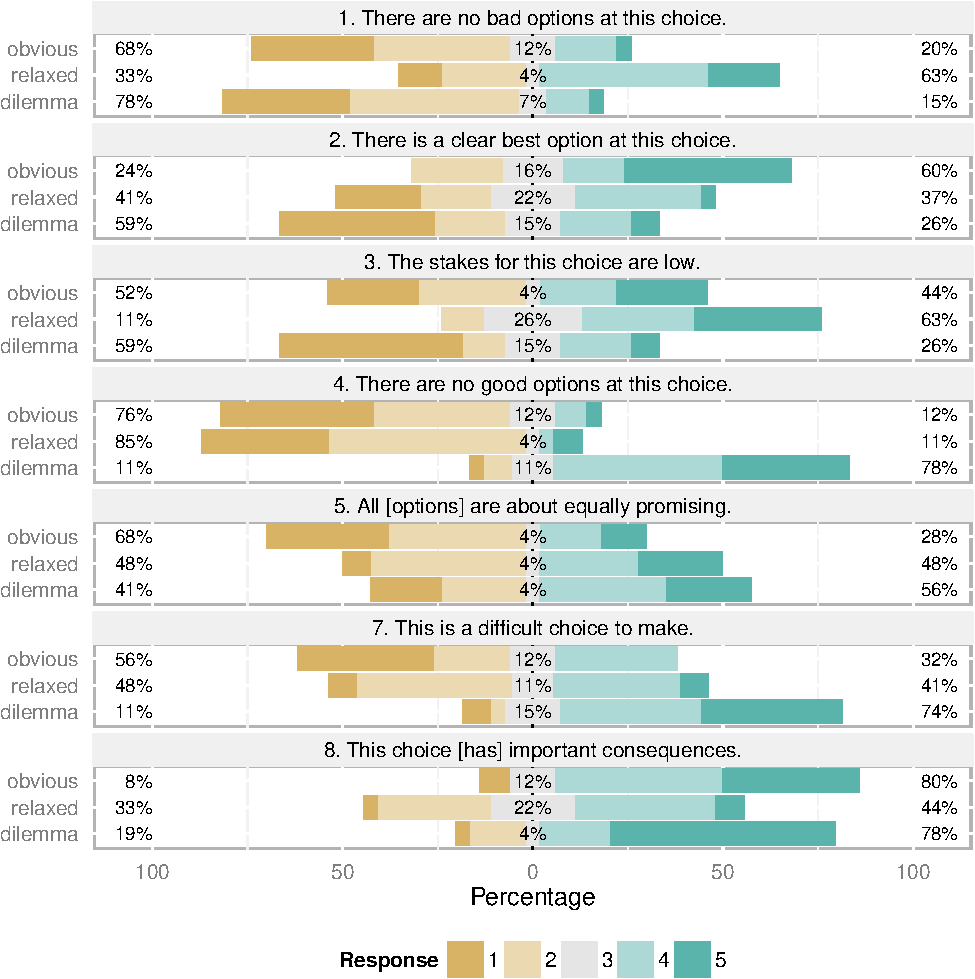
\includegraphics[width=\textwidth]{fig/combined-report-cropped.pdf}
  \caption[Prospective data summary]{A summary of the data by question plotted as percentages of respondents per treatment who gave each possible answer following \citep{Robbins2011}. Responses range from 1 (strongly disagree) to 5 (strongly agree) with 3 being ``neutral.'' Disagreeing responses are plotted to the left, and agreeing responses are plotted to the right.}
  \label{fig:e1-report}
\end{figure}

%\begin{table}[!p]
%  \centering
%\bgroup
%\def\arraystretch{1.3}
%%\setlength{\tabcolsep}{0.7em}
%%\begin{tabular}{l | p{0.5em} | p{2.2em} | p{1.8em} | p{0.5em} | p{2.2em} | p{1.8em} | p{0.5em} | p{2.2em} | p{1.8em}}
%\begin{tabular}{l | c|c|c | c|c|c | c|c|c}
%Question      & \multicolumn{3}{|c|}{Obvious} & \multicolumn{3}{|c|}{Relaxed} & \multicolumn{3}{|c}{Dilemma} \\
%\hline
%\eIqIabbr/    & \tenp & \tensig{A}{0.176} & \tesig{D}{0.009}{66\%} \\
%\hline
%\eIqIIabbr/   & \tesig{A}{0.023}{64\%}  & \tenp & \tesig{D}{0.047}{62\%} \\
%\hline
%\eIqIIIabbr/  & \tenp & \tesig{A}{0.015}{65\%}  & \tenp \\
%\hline           
%\eIqIVabbr/   & \tesig{D}{0.006}{68\%}  & \tesig{D}{0.005}{68\%}  & \tesig{A}{0.007}{67\%} \\
%\hline
%\eIqVabbr/    & \tensig{D}{0.069} & \tenp & \tensig{A}{0.322} \\
%\hline
%\hline
%\eIqVIIabbr/  & \tensig{D}{0.073} & \tenp & \tesig{A}{0.009}{66\%} \\
%\hline
%\eIqVIIIabbr/ & \tenp & \tenp & \tesig{A}{0.001}{71\%} \\
%\end{tabular}
%\egroup
%  \caption[Prospective experiment single-treatment results]{%
%Single-treatment results.
%%
%Each entry has a letter indicating the hypothesis (agree (A) or disagree (D)) followed by the $p$-value for that test.
%%
%Significant entries ($p < 0.05$) are listed in bold, and indicate a common-language effect size (the percentage of comparisons supporting the hypothesis).
%%
%Non-significant entries are highlighted in \nsighcolor/.
%%
%Note that question 6 (the trick question) is omitted here.
%}
%  \label{tab:e1-single-results}
%\end{table}

\begin{table}[!p]
\centering
{
\def\arraystretch{1.3}
\setlength{\tabcolsep}{0.4em}
\begin{tabular}{l  c  c c c  c  c c c  c  c c c}
\toprule
Question &%
 & \multicolumn{3}{c}{\eIobviousabbr/} &%
 & \multicolumn{3}{c}{\eIrelaxedabbr/} &%
 & \multicolumn{3}{c}{\eIdilemmaabbr/} \\
\midrule
\eInobadabbr/ &%
 & \tenp  &%
 & \tensig{A}{0.176} &%
 & \tesig{D}{0.009}{69\%} \\
\eIclearbestabbr/ &%
 & \tesig{A}{0.023}{66\%} &%
 & \tenp  &%
 & \tesig{D}{0.047}{63\%} \\
\eIlowstakesabbr/ &%
 & \tenp  &%
 & \tesig{A}{0.015}{67\%} &%
 & \tenp  \\
\eInogoodabbr/ &%
 & \tesig{D}{0.006}{70\%} &%
 & \tesig{D}{0.005}{70\%} &%
 & \tesig{A}{0.007}{69\%} \\
\eIbalancedabbr/ &%
 & \tensig{D}{0.069} &%
 & \tenp  &%
 & \tensig{A}{0.322} \\
\eIdifficultabbr/ &%
 & \tensig{D}{0.073} &%
 & \tenp  &%
 & \tesig{A}{0.009}{69\%} \\
\eIconsequencesabbr/ &%
 & \tenp  &%
 & \tenp  &%
 & \tesig{A}{0.001}{73\%} \\
\bottomrule
\end{tabular}

}
  \caption[Prospective experiment single-treatment results]{%
Single-treatment results.
%
Each entry has a letter indicating the hypothesis (`A' for agree or `D' for disagree) followed by the $p$-value for that test.
%
Significant entries ($p < 0.05$) are listed in bold, and indicate a common-language effect size (the percentage of comparisons supporting the hypothesis).
%
Non-significant entries are highlighted in \nsighcolor/.
%
Note that question 6 (the trick question) is omitted here.
}
  \label{tab:e1-single-results}
\end{table}


\begin{table}[!p]
\centering
\bgroup
\def\arraystretch{1.3}
\setlength{\tabcolsep}{0.7em}
\begin{tabular}{l c c c c}
\toprule
Question & Hypothesis & $p$-value & Effect \\
\toprule
\eInobadabbr/ &\tesig{relaxed$>$dilemma}{$\bm{3.1\sqtimes 10^{-4}}$}{76\%} \\
\midrule
\eIclearbestabbr/ &\tesig{obvious$>$dilemma}{$\bm{1.1\sqtimes 10^{-4}}$}{78\%} \\
\midrule
\multirow{2}{10em}{\eInogoodabbr/} &\tesig{dilemma$>$obvious}{$\bm{1.9\sqtimes 10^{-7}}$}{88\%} \\
 &\tesig{dilemma$>$relaxed}{$\bm{1.2\sqtimes 10^{-7}}$}{87\%} \\
\midrule
\eIbalancedabbr/ &\tesig{dilemma$>$obvious}{0.036}{64\%} \\
\midrule
\multirow{2}{10em}{\eIdifficultabbr/} &\tesig{dilemma$>$obvious}{$\bm{2.7\sqtimes 10^{-5}}$}{80\%} \\
 &\tesig{dilemma$>$relaxed}{0.001}{73\%} \\
\midrule
\multirow{2}{10em}{\eIconsequencesabbr/} &\tensig{dilemma$>$obvious}{0.140} \\
 &\tesig{dilemma$>$relaxed}{$\bm{3.8\sqtimes 10^{-4}}$}{75\%} \\
\bottomrule
\end{tabular}

\egroup
\caption[Prospective between-treatment results]{%
Between-treatments results.
%
Each row indicates a hypothesis, the corresponding $p$-value, and the effect size if the result is significant ($p < 0.05$). Significant results are shown in bold; non-significant results are in \nsighcolor/.
}
  \label{tab:e1-between-results}
\end{table}


A summary of the data is shown in \cref{fig:e1-report}.
%
The percentages shown are total percent of participants who disagreed, were neutral, or agreed with the given question (from left to right) and the percentages for each separate response are plotted as colored bars.
%
For each question, data from each of the three treatments is plotted separately, and in some cases divergence is immediately apparent.
%
Of course, differences that seem apparent on this summary graph may or may not be statistically significant.


I tested my hypotheses as described above, and the results of those tests are show in \cref{tab:e1-single-results,tab:e1-between-results}.
%
\Cref{tab:e1-single-results} shows the single-treatment hypothesis results: 9 of my 13 hypotheses were confirmed by my data, while 4 were not.
%
Each entry in this table indicates the hypothesis (agree $\rightarrow$ ``A'' and disagree $\rightarrow$ ``D''), the $p$-value for that hypothesis (the hypothesis is confirmed if the $p$-value is below 0.05), and if confirmed, the common-language effect size for that test.
%
\Cref{tab:e1-between-results} shows the between-treatment hypothesis results: 8 of my 9 hypotheses were confirmed by my data and 1 was not.


Note that the common-language effect size is just the percentage of comparisons between the cases being tested that support the alternate hypothesis.
%
This means that, for example, if all responses are neutral, the common-language effect size when asserting that the responses are greater than a uniform distribution will be exactly 50\% (the theoretical minimum common-language effect size).
%
This is because 50\% of comparisons between an all-neutral data set and a uniform data set will support the alternate hypothesis (that the neutral data's median is higher) and 50\% will refute it (counting tied comparisons as half-supporting and half-refuting).
%
By the same logic, if responses were all ``somewhat agree,'' the effect size would be 70\%, and if responses were all ``strongly agree,'' the effect size would be 90\% (the theoretical maximum effect size in the studies presented here).
%
The effect sizes listed in \cref{tab:e1-single-results} range from 62\% to 71\%, which are moderate to strong effects.
%
The effect sizes in \cref{tab:e1-between-results} range from 63\% to 83\%, with most being strong effects at $>$70\% effect size.


Besides the single-treatment and between-treatment hypotheses, all three of the stakes hypotheses were confirmed.
%
For the first (low-stakes choices would elicit agreement that their stakes were low) the $p$-value was 0.0047 and the effect size was 65\%.
%
The second stakes hypothesis (that high-stakes choices would elicit disagreement with the same statement) had a $p$-value of 0.0011 and an effect size of 70\%.
%
Finally, the backup hypothesis (that agreement would be higher in the low-stakes case than the high-stakes case) was a given as the first two were confirmed; it had $p = 9.7\times10^{-11}$ and an effect size of 83\%.


\section{Discussion}

Out of the 25 specific hypotheses, 20 were supported by the data.
%
This indicates that most of the perceptual qualities I expected given the constraints used to generate choices were in fact identified by most of the survey participants.
%
In particular, the fact that all of the stakes hypotheses were confirmed indicates that \dunyazad/'s author-based estimation of which player goals are more and less important is working.
%
On a treatment-by-treatment basis, the observed properties were:
%
\begin{itemize}
  \item \obv{} choices---Participants tended to agree that \obv{} choices had a clear best option (question 2) and they tended to disagree with the statement that they had no good options (question 4). I expected that participants would disagree that all of the options were equally promising (question 5) and that these choices were difficult (question 7) but in both cases the data did not confirm these expectations.
  \item \rlx{} choices---Participants tended to agree that the stakes for these choices were low (question 3) and they tended to disagree with the statement that these choices had no good options (question 4). I expected participants to agree that these choices had no bad options (question 1) but the data did not support this hypothesis.
  \item \dlm{} choices---Participants tended to disagree that there were ``no bad options'' at these choices (question 1) and agree that there were ``no good options'' at these choices (question 4). Furthermore, they disagreed with the statement that these choices had a clear best option (question 2), and agreed that these choices were difficult and had important consequences (questions 7 and 8). However, I expected participants to agree that all options at these choices were about equally promising, but the data did not support this hypothesis.
\end{itemize}
%
Overall, the data support \dunyazad/'s ability to control stakes and outcome valences, but also show that it has a bit of trouble making outcomes seem similar.
%
The areas where its choices were able to produce the desired poetic effects are important successes for automatic reasoning about choice poetics, and they imply that the goals survey participants considered when judging options align at least somewhat with those the system assumed players would have.


Places were the data did not support my hypotheses are opportunities for further scrutiny.
%
To start with, I wanted to investigate whether the failed hypotheses were the result of general trends across all choices generated under a treatment condition or whether any single choice contributed disproportionately to an unexpected result.
%
To do this I broke down the results by individual questions within a treatment and plotted them to see if there was any indication of per-question differences.


\subsection{Option Relativity}


\begin{figure}[!h]
  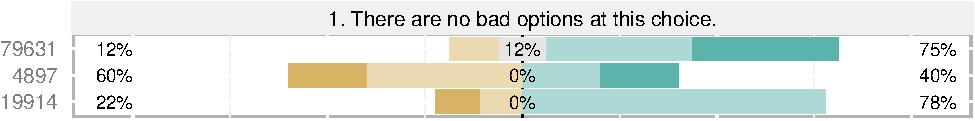
\includegraphics[width=\textwidth]{fig/relaxed-q1.pdf}
  \caption[``No bad options'' prospective responses]{A graph of responses to question 1 under the \rlx{} treatment. The three numbers are the seeds used to generate the three different choices for this treatment. The graph setup is the same as in \cref{fig:e1-report}.}
  \label{fig:e1-relaxedq1}
\end{figure}


The first of my failed hypotheses involved the \rlx{} treatment.
%
I expected the \rlx{} treatment to elicit agreement with the statement ``There are no bad options at this choice,'' but it didn't do so definitively (the statistical test failed to reject the null hypothesis that the answers to this question were consistent with a uniform distribution of underlying responses).
%
A per-choice breakdown of the data for the \rlx{} condition shown in \cref{fig:e1-relaxedq1} gives a strong indication that the question with seed 4897 elicited qualitatively different responses than the two other questions in this treatment.
%
That particular question is shown in \cref{fig:e1-seed-4897}, and reveals one possible reason for what I observed: unlike the other two questions in the \rlx{} case, option three of this question lists ``no relevant skills'' rather than giving a relevant skill possessed by the player.


\begin{figure}[!h]
\centering
\fbox{
\parbox{0.95\columnwidth}{
  \quoteshape
You come to a tavern and decide to rest for a while.
%
A noble is bored and a peasant is bored and a merchant is selling a book of herbal lore.
%
What do you do?
\begin{enumerate}[itemsep=0pt,topsep=4pt,parsep=0pt,partopsep=0pt]
\item You tell the peasant a story \\
  (You have skill: storytelling).
\item You tell the noble a story \\
  (You have skill: storytelling).
\item You offer to trade the merchant your dragon scale for the merchant's book of herbal lore \\
  (no relevant skills).
\end{enumerate}
}
}
\caption[``Relaxed'' choice 4897]{The \rlx{} choice with seed 4897 (minus the framing, which is largely the same as that shown in \cref{fig:exframing}).}
  \label{fig:e1-seed-4897}
\end{figure}


The fact that the player doesn't have any skills relevant to that action does not mean that the action will fail, but it might make that option seem less desirable than the others at that choice.
%
None of the options at the other two choices in the \rlx{} treatment listed ``no relevant skills,'' they all listed some skill that the player had as relevant, which explains why there might be a difference in responses.
%
If that wording caused the shift, it would be consistent with Schwartz et al.'s theory of satisficing versus maximizing personalities \citep{Schwartz2002} for real-world choices.
%
Schwartz et al. have found that while some people are happy as long as their choices lead to satisfactory results, others are unhappy if their choices lead to good but nevertheless suboptimal results.
%
The strong split in responses for this specific case (including both significant ``strongly disagree'' and significant ``strongly agree'' contingents) indicates that some people may be interpreting the phrase ``bad option'' as meaning options that are absolutely bad, while others may be comparing the options against each other.
%
It would take more data to discern whether this distinction is what is at work here, but it is clear that it is an important distinction for choice poetics, and it is not yet something that \dunyazad/ reasons about.


Although \dunyazad/ does not reason about this, it is to some degree aware of the distinction between the question with seed 4897 and the other two questions in that treatment.
%
The constraints for the \rlx{} condition were that each option either ``enables'' or ``achieves'' a goal (in the technical senses; see page \pageref{page:option-analysis} in \cref{page:option-analysis}), and in this case, the system generated two options that ``achieved'' a goal and one that merely ``enabled'' a goal, thus creating a distinction even on its own terms.
%
The other two questions in the \rlx{} category each included three options which ``achieved'' a goal.
%
In light of the survey results, it is clear that to construct choices that unambiguously have ``no bad options'' the system should not only require that each option works towards a player goal, but that each option is balanced against all others.

\subsection{Balancing Failures}

Another unsupported hypothesis was that in the \dlm{} treatment participants would agree with the statement ``All of the options at this choice are about equally promising.''
%
I expected this because one of the constraints of the \dlm{} treatment was that all of the threatened goals should have the same priority.
%
However, even for the individual choice in the \dlm{} treatment where participants reported the most agreement, 30\% of participants answered ``somewhat disagree.'' 


\begin{figure}[!h]
  \centering
  \includegraphics[width=0.8\textwidth,page=3]{fig/choices-cropped.pdf}
  \caption[Histogram of option preferences for ``dilemma'' choices]{A histogram of options selected by participants at the three different \dlm{} choices (each labeled by seed).}
  \label{fig:e1-dilchoices}
\end{figure}


\Cref{fig:e1-dilchoices} shows the options that participants said they would choose for the three dilemma choices.
%
For the first two choices, option two is a clear loser, and looking at the choices, it's easy to see why.
%
Both of those choices (which are nearly identical) involve being attacked by a dragon.
%
In both choices, option two is an option to attack the dragon yourself, but of course you have neither the ``fighting'' skill nor a weapon, and the dragon has both.
%
Although you also lack relevant skills for the other options, making a desperate attempt to flee from or pacify a dragon seems like a better choice than fighting it (at the very least, it did to all of my participants).


There are three factors contributing to the system's divergence from players' analysis of the options.
%
The first has to do with the granularity of expectations, the second with the granularity of goal priorities, and the third with stacking goals.


First, there are some clear arguments available to players as to why fighting might be a worse option than fleeing (for example) in an unfavorable situation.
%
One is that fighting presents a \emph{greater risk} of a bad result, and another is that fighting is directly related to a \emph{categorically worse} result.
%
The first argument has to do with the granularity of expectations: \dunyazad/ just recognizes events as \prq{unlikely}{,} \prq{neutral}{,} or \prq{likely}{.}
%
In this case, it reasons that since both fleeing and fighting are \prq{likely}{} to \prq{fail}{} the goal of avoiding the present threat, both options fail a high-priority goal.
%
However, given that all options are marked negatively, the prospect of fleeing evokes more hope for unwarranted success than the prospect of fighting.
%
This could be expressed in \dunyazad/ by introducing evaluations like \prq{somewhat\_likely}{} and \prq{very\_likely}{} that would distinguish these cases.
%
The \prq{skill\_link}{} mechanism would have to be updated to give estimates of these levels of likelihood for different actions in different circumstances, of course.


Another argument a player could make as to why fighting is worse than fleeing in this situation has to do with the relative magnitude of the results.
%
Internally, \dunyazad/ recognizes that the \prq{attack}{} option is likely to \prq{fail}{} both the \prq{avoid\_threats\_to}{} and \prq{preserve\_health}{} goals, while the \prq{flee}{} option is only expected to \prq{fail}{} the \prq{avoid\_threats\_to}{} goal.
%
However, as \dunyazad/ is written now, it treats an option that indicates one high-priority goal failure no differently form one that indicates multiple failures.
%
Particularly for choice structures which are supposed to have balanced options, some kind of counting logic would be useful to determine when one option is better or worse than another, even when they're in the same general category.


In the same vein, one could argue that even without counting how many goals fail, the \prq{preserve\_health}{} goal should be higher-priority than the \prq{avoid\_threats\_to}{} goal.
%
In part because of complexity concerns (although I have not tested this extensively) I made a decision to limit \dunyazad/ to two priority levels.
%
One could imagine instead a partially directed ``more-important-than'' graph between all player goals at each timepoint, which would be another way for \dunyazad/ to realize that fighting is worse than fleeing in this case.


The problem here is that the system's representation of player expectations is not fine-grained enough.
%
To the system, all of the options at these choices are expected to ``fail'' the player's goal of keeping their character alive and uninjured, but the system makes no distinction beyond that.
%
How certain does such failure seem to the player?
%
Exactly how badly does the player expect to fare when their goal is not met?
%
In this case, even when told that the situation is hopeless (or perhaps especially then), fleeing seemed a better option than attacking the dragon head-on, but the system doesn't distinguish those cases.
%
Based on this data, the system should be improved by adding more detail to its assessments of goal failure and success.


Any one of these corrections would help this particular case, but especially given that \dunyazad/ also has difficulty producing balanced positive options as mentioned in the previous sub-section, I suspect a more focused approach would be better.
%
After all, the likelihood reasoning \emph{is} doing a good job of predicting which options players will view positively or negatively; it just has a hard time figuring out whether options are equally positive or equally negative.
%
Rather than further overload the current reasoning, an additional subsystem dedicated to direct relative analysis of options should be added.
%
This system could separately maintain more-nuanced representations of goal priorities and outcome likelihoods, and then build arguments as to why each option is more- or less-desirable than each other option.
%
In many cases, this nuanced relative analysis could be short-circuited when the old low-fidelity analysis detects a difference.


In terms of the choice analysis method presented in \cref{ch:choice-poetics}, this exact problem was already mentioned in \cref{sec:cp-relative-option-analysis} (see the second paragraph where it talks about the balance of impacts).
%
I hypothesized here that \dunyazad/ would be able to fake a more detailed analysis by just insuring that the threatened goals had equal stakes, but that turned out not to be true.
%
In this case, what was learned from \dunyazad/'s failure backs up the theory: dilemmas are a case which needs closer inspection.
%
Getting this experimental result is still useful, because it provides a concrete example of why this is the case.


\subsection{Outcome Clarity}


\begin{figure}[!p]
  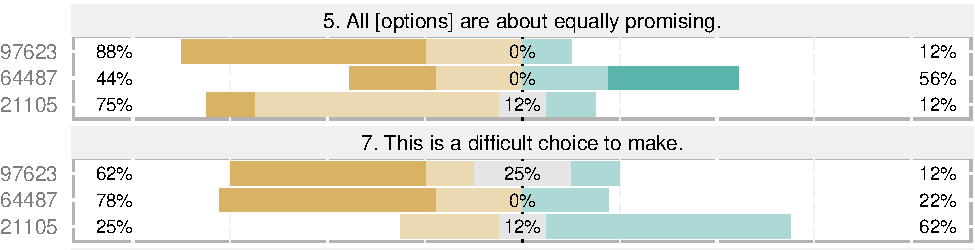
\includegraphics[width=\textwidth]{fig/obvious-q5-q7.pdf}
  \caption[Prospective balance and difficulty responses for ``obvious'' choices]{A graph of responses to questions 5 and 7 under the \obv{} treatment by seed. For question 5, the choice with seed 64487 is clearly different from the other two, and for question 7, the choice with seed 21105 is the one that stands out. \Cref{fig:e1-seed-64487,fig:e1-seed-21105} show the text of the divergent choices.}
  \label{fig:e1-obviousq57}
\end{figure}

\begin{figure}[!p]
\centering
\fbox{
\parbox{0.95\columnwidth}{
  \quoteshape
You come to a tavern and decide to rest for a while.
%
A merchant is bored and a peasant seems knowledgeable and an innkeeper seems knowledgeable.
%
What do you do?
\begin{enumerate}[itemsep=0pt,topsep=4pt,parsep=0pt,partopsep=0pt]
\item You gossip with the innkeeper \\
  (You are missing skill: negotiation).
\item You tell the merchant a story \\
  (You have skill: storytelling).
\item You gossip with the peasant \\
  (You are missing skill: negotiation)
\end{enumerate}
}
}
\caption[``Obvious'' choice 64487]{The \obv{} choice with seed 64487.}
  \label{fig:e1-seed-64487}
\end{figure}

\begin{figure}[!p]
\centering
\fbox{
\parbox{0.95\columnwidth}{
  \quoteshape
You come across some bandits attacking a merchant.
%
The bandits are threatening the merchant.
%
What do you do?
\begin{enumerate}[itemsep=0pt,topsep=4pt,parsep=0pt,partopsep=0pt]
\item You attack the bandits \\
  (They have skill: fighting. You are missing skill: fighting. They have no tool for fighting).
\item You travel onwards \\
  (no relevant skills).
\item You talk the bandits down \\
  (no relevant skills).
\end{enumerate}
}
}
\caption[``Obvious'' choice 21105]{The \obv{} choice with seed 21105.}
  \label{fig:e1-seed-21105}
\end{figure}


Not only did I expect participants to agree that options were balanced for \dlm{} choices, but I also expected them to disagree for \obv{} choices.
%
Here again my hypothesis was not supported by the data.
%
A per-choice analysis of question 5 in the \obv{} condition (the top half of \cref{fig:e1-obviousq57}) shows that again, one choice is divergent from the other two.
%
\Cref{fig:e1-seed-64487} shows that middle choice, which compared to the other two \obv{} choices is low-stakes (one of the other choices starts with a dragon attack, the other with bandits attacking some merchants).



Not only are the stakes for this choice low, but they are unclear.
%
What exactly does the player hope to gain by gossiping or by telling a story?
%
Perhaps friendship or some useful information, but those potential rewards seem both uncertain (even given a ``successful'' action) and questionably useful.
%
In contrast (albeit a contrast that participants did not see directly) the utility of fleeing from an attacking monster is clear, even if it is uncertain whether you will succeed.
%
Furthermore, there aren't any obvious risks associated with options 1 and 3, so even if the player is missing a relevant skill, they might still be worth trying.
%
Given this combination of low stakes, a dubious reward for the most-successful-seeming option, and seemingly consequence-free options all around, it is not hard to see how some might find these options ``about equally promising.''


On the other hand, the system's attempt to construct an obvious choice in this case was still somewhat successful.
%
7 of 9 participants who saw this choice ``strongly agreed'' with the statement ``There is a clear best option at this choice'' and 8 of those 9 picked option \#2 as the option they would choose.
%
While it might seem like a contradiction to agree (as 3 participants did) with both the statement that a choice has equally promising options and the statement that it has a clear best option, this highlights the difference between outcomes-focused evaluation of individual options and choice-oriented option comparison.
%
The phrasing of ``All of the options at this choice are about equally promising,'' suggests evaluating each option independently and comparing those values roughly.
%
In contrast, ``There is a clear best option at this choice,'' suggests comparing the options against each other to find one that is better than the others.
%
The fact that people often make decisions inconsistent with simple utility calculation is well-known (see e.g., \citep{Tversky1993}), so it should not be surprising that a context in which someone is asked to make a decision might elicit a different response than a context in which someone is asked to rate responses.


The implications for choice poetics are interesting, because choice poetics is concerned with both mindsets.
%
At least in terms of impact on the player, there's clearly a difference between a choice where all of the options seem ``about equally promising'' and where that's definitely not the case, even if both choices have ``a clear best option.''
%
Choices where options seem equally promising but most players choose a particular route regardless might even be good candidates for the focus of regret.
%
For example, if it turns out that the ``clear best option'' leads to failure and players are forced to revisit the original decision, having seen some potential in the alternatives they're more likely to feel that the choice was fair, and thus presumably blame their own decision for the consequences (\cref{sec:results-about-regret} discusses some data relevant to this point that resulted from the experiment on outcome evaluations).
%
At the same time, if the designer can be confident that most players will go down the ``obvious'' route first even without making the contrast with the other options huge, they can assume that most players will experience the regretful path as opposed to choosing the ultimately correct option the first time.


Despite the interesting revelations prompted by this case, \dunyazad/ does actually have a problem here: it is analyzing outcomes according to the game mechanics that it knows about, but the players in this case aren't playing a game: they're experiencing a single choice with very little context.
%
If someone had played a few of \dunyazad/'s output stories already, they'd have a view of the possibility space much more similar to \dunyazad/'s, especially in terms of the outcomes of actions like \prq{gossip}{} and \prq{tell\_story}{.}
%
If the players knew what to expect from both success and failure at these actions, and had a stronger sense of the role skills play in determining outcomes, they wouldn't get their hopes up, and the choice \emph{would} be ``obvious.''


That is the deeper issue here as well: the simple notions of ``success'' and ``failure'' when performing an action often don't correspond to overall positive an negative results when an action isn't clearly oriented towards some pressing player goal.
%
For example, an attempt to ``gossip'' despite lacking the relevant skill seems like it might still yield interesting results, and it isn't likely to be disastrous.
%
The same is not true of attacking an enemy: when they're more skilled or better-armed, there's a clear sense of danger (and of what is at stake).
%
In other words, \dunyazad/ is doing a good job of manipulating player expectations when it is heavy-handed, threatening high-priority player goals to make options appear hopeful or doomed.
%
However, when \dunyazad/ attempts to use low-priority goals in the same fashion, players don't follow its lead: ``My gossiping probably won't go `as intended?' Well, it might still be awesome!''


The simplest response to this is to just tread carefully when creating using low-stakes choices and assume that some of them aren't going to get the result you want, while making sure to use high-stakes choices if a particular property like obviousness is critical.
%
In the longer term, \dunyazad/ should recognize things like the desire to explore rather than always travel the beaten path (especially when the stakes are low).
%
At the same time, one area for future work is goal-probing questions, which would allow \dunyazad/ to ask the player (either directly or indirectly) to indicate their goals.
%
These questions would serve two purposes: first, they would allow \dunyazad/ to dynamically determine which goals (including low-priority goals) the player thinks are important.
%
Second, these questions, when successful, may subtly influence players by committing them to a goal: one a player affirms a goal, they may be more likely to behave in a manner consistent with that goal in the future (see e.g., \citep{Hall2012} on the powerful instinct for post-hoc justification when an opinion is perceived---even incorrectly---to be one's own).


\subsection{Conflicting Goals}


My hypothesis that respondents would not find \obv{} choices difficult highlights a different choice in the \obv{} category.
%
The data did not support this hypothesis, and as shown in \cref{fig:e1-obviousq57}, the choice with seed 21105 accounts for the majority of all responses that contradict it.
%
That choice is shown in \cref{fig:e1-seed-21105}, and from the system's perspective, it satisfies the definition of an obvious choice (see \cref{tab:prospective-impressions}) because the second option ``achieves'' a player goal, while neither the first nor the third do, and both the first and third ``threaten'' a player goal.


The perceived difficulty of this decision probably stems from the fact that it pits two player goals against one another: the goal of self-preservation is best served by option two, but the goal of helping others in need is best served by one of the other options.
%
This is similar to the lack of distinction between threatening one and two goals encountered above.
%
Even when one option at a choice clearly has the most-positive outcome for the player considering all goals to be equal, when that choice pits multiple goals against one another, it may be very difficult indeed.
%
In fact, choices with these structures may give rise to an entirely different set of poetic concerns that involves moral judgements (this is exactly how morality thought experiments like the ``trolley problem'' are constructed, for example---see \citep{Thomson1976}).
%
A difficult decision between two desirable or undesirable outcomes feels completely different from a decision between two outcomes each justified by competing moral principles, and it can resonate powerfully to the broader narrative structures of a story.
%
In its current state, \dunyazad/ doesn't reason about morality at all: it makes no distinction between goals in terms of their root motivations, and it has no compunction about how a result is achieved as long as no player goals are threatened in the process.
%
While \dunyazad/ gets perhaps surprisingly far without these capabilities, they're clearly important and can come up by accident even when \dunyazad/ isn't trying to make use of them.


That said, a detailed inspection of the answer set that resulted in this choice reveals another problem with the system: ignoring the lack of moral reasoning, it's simply not working as intended.
%
In this case, \dunyazad/ actually thinks that travelling onwards serves the goal of preventing the threat to the merchant (because if the player travels onwards, that entire situation is left behind and therefore the threat no longer exists) while it has no conception that this serves a goal of self-preservation (although it understands that interfering by either means threatens the player's safety).
%
There are thus two more changes to the system suggested by this data: first a bug-fix related to the consequences of travelling onwards, and second, the addition of relative goal relevance across options: the idea that if all but one option threatens an important goal, then the remaining option can be seen as indirectly supporting that goal even if none of its outcomes directly further that goal.
%
Without running this experiment, I would eventually have found and fixed the ``travel onwards'' bug, but I may not have thought to make the second change.
%
In this case, the data served to help find and diagnose an anomaly in my system, which turned out to involve an error in the code, but at the same time also pointed to two future goals for the choice structure model: adding explicit moral reasoning, and a notion of relative goal relevance when all but one option relates to a goal in the same way.


\subsection{Stakes and Consequences}

The final unsupported hypothesis was that participants would feel more strongly that \dlm{} choices had important consequences than that \obv{} choices did.
%
This hypothesis was based on the idea that consequences might seem more relevant (and thus important) when a decision was more difficult.
%
Given that one of my \obv{} choices seemed difficult to many participants as discussed above, it is unsurprising that this hypothesis was not supported.


\begin{figure}[!h]
  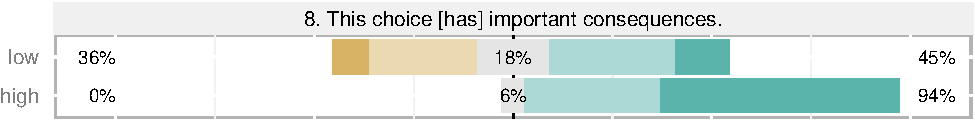
\includegraphics[width=\textwidth]{fig/stakes-q8.pdf}
  \caption[Prospective consequences results by stakes]{A graph of responses to question 8 across all treatments by stakes.}
  \label{fig:e1-stakesq8}
\end{figure}


What is interesting is the effect of the choice stakes on this question.
%
The similar hypothesis that participants would agree more in the \dlm{} case than the \rlx{} case \emph{was} supported by the data, and one big difference between those two treatments is the stakes associated with them.\footnote{A statistical analysis of the assertion that participants agree more with the statement that a choice's stakes are low in the \rlx{} case than the \dlm{} case (not one of my original hypotheses) reveals a strong significant effect ($p = 2.88\times10^{-5}$; effect size 76\%).}
%
In fact, when analyzing the data for question 8 according to stakes rather than the three treatments, high-stakes choices overwhelmingly seem as if they will have important consequences, while low-stakes choices are mixed (see \cref{fig:e1-stakesq8}).


Statistics confirm the obvious: not only did the high-stakes condition elicit significantly more agreement on question 8 than the low-stakes condition ($p = 2.14\times10^{-8}$; effect size 79\%), it was also significantly above a uniform distribution ($p = 4.9\times10^{-6}$; effect size 78\%).
%
Because all of the \rlx{} choices were low-stakes by design, there is of course correlation between the stakes and the treatments, but the 35 high-stakes cases were about evenly distributed between the \obv{} and \dlm{} treatments (16 in \obv{} and 19 in \dlm{}).
%
Such an overwhelming effect (none of the 35 respondents who saw a high-stakes choices thought it would \emph{not} have important consequences) further indicates that the system is successful in predicting high-stakes player goals: for 94\% of choices where the system thought that an important player goal was affected, players agreed at least somewhat that the consequences seemed important.


\section{Conclusions}

Overall, this study confirmed \dunyazad/'s ability to construct choices based on player expectations when certain criteria are met.
%
Notably, many of the failed hypotheses involved situations where several options together affected how a choice was perceived:
%
\begin{itemize}
  \item For question 1 (``There are no bad options at this choice.'') relative rather than absolute judgements of what is a ``bad'' option may have come into play.
  \item For question 5 (``All of the options at this choice are about equally promising.'') it seems \dunyazad/ may need to make finer distinctions between different modes of goal failure, as several options expected to lead to failure may still seem to offer a range of possibilities when no better options are present.
  \item Question 7 (``This is a difficult choice to make.'') showed that a choice can be difficult when multiple goals conflict, even when expectations for one goal are much better than for another.
\end{itemize}
%
These results point to several possible improvements for \dunyazad/, and collectively reinforce the importance of considering choices holistically when evaluating choice poetics.


As already discussed, there are a number of changes that could be made to \dunyazad/ based on these results:
%
\begin{itemize}
  \item Implement separate ``satisfaction'' and ``maximization'' player decision modes so that the system can reason about how difficult a decision might seem, whichever decision modality a player is using.
  \item Upgrade \dunyazad/'s system for estimating how individual options affect goals by adding more detail so that it can further distinguish different magnitudes of risk and reward.
  \item Have \dunyazad/ represent players' uncertainty about the possible outcomes of actions like ``gossip'' and ``tell story'' so that it can have a clearer picture of which options seem promising in low-stakes situations.
  \item Implement goal-probing questions (either direct or indirect) that allow the system to gain direct knowledge about player goals, especially for low-stakes options. This would also allow \dunyazad/ to further support role-playing by allowing different players to choose options which imply different goals or goal priorities.
  \item Implement a model of goal conflicts and more detailed relative goal priorities including moral reasoning.
  \item Implement the idea of relative goal relevance: if all but one option at a choice either threatens or enables a goal, then the remaining option implicitly does the opposite.
\end{itemize}
%
These changes could make \dunyazad/ even more successful at constructing choices which produce particular player expectations (and thus which can produce specific poetic effects).
%
They are also in line with my goal of getting \dunyazad/ to generate choices with more complex poetics, such as choices that elicit regret or prompt deliberation.


One important functionality of \dunyazad/ not tested in this first study was its ability to judge outcomes.
%
This study did largely verify that \dunyazad/'s player expectations about options are working, and it can generate outcomes that both support and betray those expectations.
%
The experiment described in \cref{ch:outcome-results} relies on this functionality to test how accurate \dunyazad/'s estimates of retrospective perceptions are.

\chapter{Experiment II: Retrospective Impressions}

\label{ch:outcome-results}

This chapter describes results from a second study involving \dunyazad/, this time scrutinizing player's impressions of a choice \emph{after} making a decision.
%
The setup is largely the same as the first experiment, so reading \cref{ch:option-results} will help to understand the results presented here.
%
In particular, \cref{sec:e1-method} describes the experimental procedures used in the first experiment, which were largely the same in this experiment, and \cref{sec:e1-hypotheses} describes how hypotheses were tested in the first experiment, which was also largely replicated in this experiment.


Key results echo those from \cref{ch:option-results} in that \dunyazad/ needs to be able to reason better about conflicting goals and use more detailed goal priorities.
%
Additionally, results relevant to outcome perspectives show that \dunyazad/ might do well to adopt a strategy that reasons explicitly about (and/or explicitly constructs) option implications.
%
The current system which automatically assumes option implications based on \dunyazad/'s internal representation of actions and their potential consequences in some cases does not align with the expectations that players seem to develop based on the actual text generated for the options.
%
These results and others, along with the results from the experiment described in \cref{ch:option-results}, have implications for the goal-based choice analysis technique presented in \cref{sec:goal-based-choice-analysis} as well, and these are discussed in \cref{sec:results-prospective-caveats}.


\section{Overview}


Because the results from testing \dunyazad/'s prospective impression subsystem were largely successful, I ran another experiment to test the retrospective impression system.
%
In this experiment both prospective and retrospective impression constraints were used to create six kinds of choices defined in terms of their prospective and retrospective impressions (see \cref{tab:prospective-impressions,tab:retrospective-impressions,tab:dunyazad-outcome-feel-structures}):

\begin{itemize}
  \item \lbl{Expected Success}---These choices have three options which present themselves as leading to success, and each option has a successful outcome. In terms of \prq{outcome\_feel}{} values (see \cref{tab:dunyazad-outcome-feel-structures}) each option at these choices is an \exps{} option. No matter which option a participant selects, they will be picking an option that suggests success, and they will get a successful outcome (as far as \dunyazad/ understands things).
  \item \lbl{Expected Failure}---The opposite of expected success: every option suggests and results in failure. Internally, each option is an \expf{.}
  \item \lbl{Unexpected Failure}---These choices consist of three \prq{unfair}{} options. In other words, each option seems as though it will be successful, but each ultimately results in failure. These choices should appear largely the same as \exps{} choices before an option is chosen.
  \item \lbl{Unexpected Success}---The opposite of unexpected failures, these choices consist of three \prq{miracle}{} options---each indicates failure but results in success. These choices mimic ``expected failure'' options until the player selects an option and sees an outcome.
  \item \lbl{Obvious Success}---These choices have a single \exps{} option and two \expf{} options, forming an \obv{} \prq{option\_structure}{.} The outcomes of each choice align with what the option text suggests: the ``good'' option leads to success and the others lead to failure.
  \item \lbl{Obvious Failure}---These choices have a single \prq{unfair}{} option and two options which are either \prq{miracle}{}s or \prq{nice\_gamble}{}s. Just like ``obvious success'' choices, their \prq{option\_structure}{} is \obv{.} Of course, instead of leading to the expected results, each option results in the opposite of what it suggests.
\end{itemize}

These six choice structures were designed to manipulate three variables: valence of outcomes, expectedness of outcomes, and the presence of viable alternatives.
%
Note that due to the study design, each participant only ever saw a single choice, they could not form judgements based on comparing choices across categories.
%
The bulk of the hypotheses were designed simply to verify that the participants agreed with \dunyazad/'s internal evaluation of these variables, but there were a few hypotheses designed to probe for possible relationships between these six conditions.
%
Overall the results show that \dunyazad/ did a good job producing positive outcomes, but struggled with negative outcomes, and (partially as a result of this) had some trouble producing unexpected results.
%
Despite these problems, the data reveal some interesting interactions between the three underlying variables, such as a difference in satisfaction based on the presence or absence of viable alternatives and a relationship between the valence of unexpected outcomes and their perceived fairness.


\section{Method}

The experimental setup for this experiment was largely the same as the setup for the prospective impressions experiment described in \cref{ch:option-results}.
%
This section lists the major differences between the two setups but does not reiterate the details of the original setup (see \cref{sec:e1-method}) that were unchanged.
%
The first obvious difference was the sample size.
%
As already mentioned, there were six types of choice generated, rather than 3, for a total of 18 choices (three per condition, just as in the original experiment).
%
Instead of showing each choice to 10 subjects, each choice was shown to 15 subjects, which meant that there were nominally 270 participants instead of 90.
%
Luckily the use of Amazon Mechanical Turk means that there is very little effort per participant, so the logistics of the second study weren't drastically different from those of the first.


\subsection{Extra Constraints}

In an attempt to avoid some of the problems with low-stakes choices in the original experiment, every choice in this experiment was required to have high stakes.
%
Furthermore, rather than allowing \dunyazad/ to pick any setup it wanted, the three choices in each condition were generated using fixed setups (\prq{market}{,}, \prq{monster\_attack}{,} and \prq{threatened\_innocents}{}).
%
This helped insure that the setup text wasn't a significant variable between the cases, and that each case would include a variety of setups.
%
Setup parameters were still allowed to vary freely; the \prq{market}{} setup in particular has multiple possible configurations.


\subsection{Framing}

Unlike the first survey, where participants were asked to pick the option that they ``would have chosen,'' participants in this study were instructed:
%
``Please read the following short story which presents you with a choice, make a decision, and then answer the questions about that choice below.''
%
The choices were presented with a radio button next to each option, and hovering over the text of each option highlighted it.
%
When the participant clicked anywhere over the text of an option, the outcome text for that option would be displayed in the space directly below it (moving any following options down).
%
At the same time, the selected option text and the outcome text were highlighted in bold and the radio button for the selected option was filled in, while the non-selected options were faded to gray and their radio buttons were disabled.
%
Once an option was selected the highlight-on-hover and click-to-choose functionality were disabled.
%
Immediately before the option texts the phrase ``To choose, click on an option below. Once you make a decision you will not be able to change it,'' appeared to make sure that participants understood the format.
%
The option selected by the player was recorded as part of the study data; every single participant selected an option and thus saw an outcome.


Of course, although this decision mechanism mimicked the decision-making environment of modern browser-based narrative choice games, it meant that participants would see the outcome of their decision before answering questions about the options that they had.
%
This approach was chosen intentionally to maintain the flow of the setup into the choice; asking a set of survey questions after seeing the choice but before making a decision would have an impact on the poetics of the choice.
%
Of course, having seen an outcome inevitably changes one's perception of an option (especially if that outcome was unexpected).
%
The data in the first survey therefore is more informative about option-related poetics.
%
To counteract this somewhat, the following text appeared before the option questions:
%
``For these questions, consider just the options presented, and ignore the outcome of the option that you chose.''
%
Complying with such a request is not entirely possible, of course, but the option-related questions in this survey were only present to establish a point of comparison with the first study, and were not the focus of the results.


\subsection{Compensation}

Participants were still Amazon Mechanical Turk workers, but for this study, each participant was paid \$2.00 instead of \$0.50.
%
This was partially because this study involved more questions, and partially because of the desire to pay more fairly for participants' time.
%
Based on the quality of the responses that I received and on reviews of the tasks posted on \url{https://turkopticon.ucsd.edu/}, I believe that this level of pay was satisfactory both from my own perspective and from the perspective of the participants.
%
The total cost of the experiment including fees paid to Amazon and the costs of pilot tasks (4 pilot tasks were posted to debug the survey before posting the 270 main tasks) was \$765.20.


\subsection{Questions}

Of course, one major difference between the studies was the set of statements included.
%
This study had three sections: statements about the options, statements about the outcome, and statements about motivation.
%
The option statements were actually a subset of the statements from the original survey, with extra text to encourage participants to think only about the options and ignore the outcome as mentioned above.
%
The following five option statements (listed by their internal labels) were included: \\[0.3\baselineskip]
%
{
  \setstretch{1.0}
  \mydef{5em}{\raggedleft\textbf{\eIIoptobviousabbr/}}{\hangparas{1.5em}{1}\quoteshape 1. ``Considering just the options, there seems to be a clear best option at this choice.''} \\
  \mydef{5em}{\raggedleft\textbf{\eIIoptbalancedabbr/}}{\hangparas{1.5em}{1}\quoteshape 2. ``Ignoring outcomes, the options at this choice all seem about equally good (or bad).''} \\
  \mydef{5em}{\raggedleft\textbf{\eIIoptnobadabbr/}}{\hangparas{1.5em}{1}\quoteshape 3. ``Ignoring outcomes, there are no options that seem bad at this choice.''} \\
  \mydef{5em}{\raggedleft\textbf{\eIIoptnogoodabbr/}}{\hangparas{1.5em}{1}\quoteshape 4. ``Ignoring outcomes, none of the options at this choice seem good.''} \\
  \mydef{5em}{\raggedleft\textbf{\eIIoptstakesabbr/}}{\hangparas{1.5em}{1}\quoteshape 5. ``Considering just the options, the stakes for this choice seem low.''} \\
}


In addition to option statements, this survey included statements about the outcome that participants saw: \\[0.3em]
%
{
\setstretch{1.0}
\mydef{7em}{\raggedleft\textbf{\eIIoutfairabbr/}}{\hangparas{1.5em}{1}\quoteshape 1. ``Given the options available, the outcome I got is fair.''} \\
\mydef{7em}{\raggedleft\textbf{\eIIoutsenseabbr/}}{\hangparas{1.5em}{1}\quoteshape 2. ``The outcome that I got makes sense given the option that I selected.''} \\
\mydef{7em}{\raggedleft\textbf{\eIIoutbadabbr/}}{\hangparas{1.5em}{1}\quoteshape 3. ``I got a bad outcome.''} \\
\mydef{7em}{\raggedleft\textbf{\eIIouthappyabbr/}}{\hangparas{1.5em}{1}\quoteshape 4. ``I'm happy with the option that I chose.''} \\
\mydef{7em}{\raggedleft\textbf{\eIIoutunfairabbr/}}{\hangparas{1.5em}{1}\quoteshape 5. ``The outcome that I got is unfair, given the options available.''} \\
\mydef{7em}{\raggedleft\textbf{\eIIoutunexpectedabbr/}}{\hangparas{1.5em}{1}\quoteshape 6. ``The outcome that I got is completely unexpected.''} \\
\mydef{7em}{\raggedleft\textbf{\eIIouttrickabbr/}}{\hangparas{1.5em}{1}\quoteshape 7. ``There is an outcome.'' (This is a trick question to test whether you're paying attention. Please simply indicate that you are in complete \emph{disagreement}.)} \\
\mydef{7em}{\raggedleft\textbf{\eIIoutbrokenabbr/}}{\hangparas{1.5em}{1}\quoteshape 8. ``There might be a problem with this choice---the outcome I got does not make sense.''} \\
\mydef{7em}{\raggedleft\textbf{\eIIoutgoodabbr/}}{\hangparas{1.5em}{1}\quoteshape 9. ``The outcome that I got is a good outcome.''} \\
\mydef{7em}{\raggedleft\textbf{\eIIoutexpectedabbr/}}{\hangparas{1.5em}{1}\quoteshape 10. ``I pretty much expected the outcome that I got.''} \\
\mydef{7em}{\raggedleft\textbf{\eIIoutregretabbr/}}{\hangparas{1.5em}{1}\quoteshape 11. ``I wish I had chosen a different option.''} \\
}
%
Underlying these statements were 5 concepts which were each addressed by a pair of statements with counterbalanced answers.
%
These underlying concepts were: \textbf{fairness} (questions 1 and 5), \textbf{sense} (questions 2 and 8), \textbf{valence} (questions 3 and 9), \textbf{satisfaction} (questions 4 and 11), and \textbf{expectedness} (questions 6 and 10).
%
The order of the questions was scrambled and chosen such that no pair of complimentary statements would appear adjacent to each other in order to encourage subjects to approach each question individually.


Although the outcome questions were the main focus of this study, some questions asking participants to self-report their motivations were added at the end of the study to get direct feedback about modes of engagement.
%
These questions were prefaced with the prompt:
%
\begin{quote}
  \quoteshape
Please answer the following questions about your motivations for making the decision you made, as well as about your motivations and goals in general when playing/reading interactive stories.
\end{quote}
%
The first question asked directly about motivation:
%
\begin{quote}
  \quoteshape
  1. Which of the following motive(s) contributed to your decision? (pick one or more) \\
  %
  (Note: no submissions will be rejected based on this information; wanting to get this survey done quickly is a perfectly valid reason for making a decision.) \\
  \begin{itemize}
    \item[\ding{111}] I'm taking an online survey. I just chose an option quickly so that I could complete the survey.
    \item[\ding{111}] I was just curious to find out what would happen if I chose the option I did.
    \item[\ding{111}] I imagined a character in the story situation and chose what that character would do.
    \item[\ding{111}] I chose what I would have chosen were I in the situation described in the story.
    \item[\ding{111}] I chose the option that I thought would lead to the most interesting/satisfying result.
    \item[\ding{111}] I looked at the skill information and chose the option that I thought would be most successful.
    \item[\ding{111}] Other (please explain):
  \end{itemize}
\end{quote}
%
A free text area was provided below the ``Other'' option.
%
As suggested in the prompt, participants were free to select more than one option or leave them all blank.
%
Note that the options here mostly correspond to the modes of engagement proposed in \cref{ch:choice-poetics}.
%
Of course, by providing exactly these options players may be subconsciously coerced into aligning their motivations with the archetypes that I have defined, and so the results of this study shouldn't be taken to be a confirmation that player motivations \emph{do} fit into the theoretical framework discussed above.
%
However, the relative frequency of different responses still provides some information about whether players' motives are diverse or generally similar, for example.
%
The responses to this question were labelled respectively as \pr{speed}, \pr{curious}, \pr{role}, \pr{avatar}, \pr{interest}, \pr{power}, and \pr{other}.

In a similar vein, the next question asked how players evaluate outcomes:
%
\begin{quote}
  \quoteshape
  2. Which of the following judgement(s) contributes to how you generally define a ``good'' outcome in interactive experiences like the one you just played? (pick one or more) \\
  \begin{itemize}
    \item[\ding{111}] I feel an outcome is good when something good happens to my character in the story world.
    \item[\ding{111}] I feel an outcome is good if it is an interesting development in the story.
    \item[\ding{111}] I feel an outcome is good when it fits the role that I am building for my character.
    \item[\ding{111}] I feel an outcome is good when it makes my character more powerful.
    \item[\ding{111}] I feel an outcome is good when it makes progress towards beating a game.
    \item[\ding{111}] Other (please explain):
  \end{itemize}
\end{quote}
%
These responses were labelled respectively as \pr{avatar}, \pr{interest}, \pr{role}, \pr{power}, \pr{progress}, and \pr{other}.
%
Directly following was effectively the same question but for ``bad'' outcomes:
%
\begin{quote}
  \quoteshape
  3. Which of the following judgement(s) contributes to how you generally define a ``bad'' outcome in interactive experiences like the one you just played? (pick one or more)
  \begin{itemize}
    \item[\ding{111}] I feel an outcome is bad when something bad happens to my character in the story world.
    \item[\ding{111}] I feel an outcome is bad if it doesn't develop the plot.
    \item[\ding{111}] I feel an outcome is bad when my character doesn't do what I expected them to do.
    \item[\ding{111}] I feel an outcome is bad when my character expresses a value or opinion that is different from what I wanted them to express.
    \item[\ding{111}] I feel an outcome is bad when it makes my character less powerful.
    \item[\ding{111}] I feel an outcome is bad when it prevents me from making progress towards beating a game.
    \item[\ding{111}] Other (please explain):
  \end{itemize}
\end{quote}
%
These responses were labelled as \pr{avatar}, \pr{interest}, \pr{no.control}, \pr{value.clash}, \pr{power}, \pr{progress}, and \pr{other}.

The final question in the motives section asked about consistency of motives.
%
Unlike the other questions in this section, it forced participants to select a single response (although it still had an ``other'' response):
%
\begin{quote}
  \quoteshape
  4. Do you feel you approach all interactive experiences (e.g., Choose-Your-Own-Adventure novels, video games, tabletop role-playing games, etc.) with a consistent set of motivations and judgements, or do your motivations and judgements change from story to story?
  \begin{itemize}
    \item[\ding{109}] I feel that my motivations and judgements are the same no matter what interactive story I'm playing.
    \item[\ding{109}] I feel that my motivations and judgements change from story to story.
    \item[\ding{109}] I don't play interactive stories often enough to have a definite answer.
    \item[\ding{109}] Other (please explain):
  \end{itemize}
\end{quote}
%
The responses to this question were labelled \pr{consistent}, \pr{variable}, \pr{no.exp}, and \pr{other}.
%
Although the questions in the motivation section weren't subject to any statistical tests, they provide some informal information about how players approach choices.
%
A further experiment designed to seriously investigate player motivations would require a much tighter design, and would likely derive no benefit from using \dunyazad/ to generate its choices, as \dunyazad/ isn't designed to be aware of, or work with, modes of engagement.


Unlike the first survey, this survey included an optional text area at the end for any additional feedback participants wanted to share.
%
This additional feedback was not analyzed, but responses were used to help with approval decisions (several participants indicated honest confusion about some aspect of the age/fluency question; their responses were accepted).


Besides these differences, the details of this survey were the same as the first survey, including the format of response options and the framing of the various sections.
%
Of course, this survey included a different set of hypotheses.

\section{Hypotheses}

The hypotheses in this study were tested in largely the same way as those in the prospective study.
%
Each ``agree'' or ``disagree'' hypothesis was tested by comparing the results under a given condition with a uniform distribution of responses using a Mann-Whitney-Wilcoxon U test with an appropriate alternate hypothesis.
%
A uniform distribution with 35 elements was used for all comparisons, as this was the multiple of five (the number of response categories) closest to the number of samples in most of the relevant cases (32-36 for each condition, although as low as 8 in some sub-conditions; these low-$n$ comparisons are discussed where they appear).
%
For between-condition hypotheses, the two sample populations were compared directly using Mann-Whitney-Wilcoxon U tests.
%
In all cases, results are taken to be significant when their $p$-values are $<$0.05, and common-language effect sizes (see \cref{sec:e1-results} for an explanation) are indicated when results are significant.


\begin{table}[!b]
\centering
\bgroup
\def\arraystretch{1.3}
\setlength{\tabcolsep}{0.6em}
\begin{tabular}{r c c c}
\toprule
\multirow{2}{5em}{\centering Question} &%
 \eIIexpectedsuccessabbr/ &%
 \eIIobvioussuccessabbr/ &%
 \eIIexpectedfailureabbr/ \\
&%
 \eIIunexpectedfailureabbr/ &%
 \eIIobviousfailureabbr/ &%
 \eIIunexpectedsuccessabbr/ \\
\midrule
\eIIoptobviousabbr/ &%
 disagree\lc/ &%
 agree &%
 disagree\lc/ \\
\eIIoptbalancedabbr/ &%
 agree\lc/ &%
 disagree &%
 agree\lc/ \\
\eIIoptnobadabbr/ &%
 agree\lc/ &%
 disagree &%
 disagree \\
\eIIoptnogoodabbr/ &%
 disagree &%
 disagree &%
 agree \\
\eIIoptstakesabbr/ &%
 disagree &%
 disagree &%
 disagree \\
\bottomrule
\end{tabular}

\egroup
\caption[Retrospective option hypotheses]{Hypotheses about option statements in the retrospective study. Each entry corresponds to two hypotheses: one for each condition listed in the header of that column. Because the two conditions in each column share option structures, they are predicted to elicit identical responses to the option-related statements. Low-confidence hypotheses are marked with a `\lc/'.}
  \label{tab:e2-option-hypotheses}
\end{table}


\subsection{Option Hypotheses}


The three option structures used in this study were \prq{positive\_alternatives}{,} \prq{negative\_alternatives}{,} and \obv{,} as described above.
%
Each option structure corresponded to two conditions with different outcomes.
%
These paired conditions are listed in the header of \cref{tab:e2-option-hypotheses}; each option structure was predicted to yield a different set of answers to the five option statements, as shown in that table.
%
These 30 hypotheses (5 statements $\times$ 3 option structures $\times$ 2 conditions per structure) were meant to check whether \dunyazad/ was producing the desired option structures successfully.


Given the results of the first experiment, several of these hypotheses were not expected to be supported by the data.
%
These tentative hypotheses are marked with `\lc/'s in \cref{tab:e2-option-hypotheses}.
%
In particular, hypotheses having to do with options being balanced or there being no clear best option were not expected to be well-supported by the data.


\subsection{Basic Outcome Hypotheses}

\begin{table}[!p]
\centering
\bgroup
\def\arraystretch{1.3}
\setlength{\tabcolsep}{0.6em}
\begin{tabular}{r  c c}
\toprule
\multirow{2}{5em}{\centering Question} &%
 \eIIexpectedsuccessabbr/ &%
 \eIIunexpectedsuccessabbr/ \\
&%
 \eIIobvioussuccessmainabbr/ &%
 \eIIobviousfailurealtabbr/ \\
\midrule
\eIIoutfairabbr/ &%
 agree &%
 agree \\
\eIIoutunfairabbr/ &%
 disagree &%
 disagree \\
\eIIoutsenseabbr/ &%
 agree &%
 agree \\
\eIIoutbrokenabbr/ &%
 disagree &%
 disagree \\
\eIIoutgoodabbr/ &%
 agree &%
 agree \\
\eIIoutbadabbr/ &%
 disagree &%
 disagree \\
\eIIouthappyabbr/ &%
 agree &%
 agree \\
\eIIoutregretabbr/ &%
 disagree &%
 disagree \\
\eIIoutexpectedabbr/ &%
 agree &%
 disagree \\
\eIIoutunexpectedabbr/ &%
 disagree &%
 agree \\
\midrule
\multirow{2}{5em}{Question} &%
\eIIexpectedfailureabbr/ &%
\eIIunexpectedfailureabbr/ \\
&%
\eIIobvioussuccessaltabbr/ &%
\eIIobviousfailuremainabbr/ \\
\midrule
\eIIoutfairabbr/ &%
 agree &%
 disagree \\
\eIIoutunfairabbr/ &%
 disagree &%
 agree \\
\eIIoutsenseabbr/ &%
 agree &%
 disagree \\
\eIIoutbrokenabbr/ &%
 disagree &%
 agree \\
\eIIoutgoodabbr/ &%
 disagree &%
 disagree \\
\eIIoutbadabbr/ &%
 agree &%
 agree \\
\eIIouthappyabbr/ &%
 - &%
 disagree \\
\eIIoutregretabbr/ &%
 - &%
 agree \\
\eIIoutexpectedabbr/ &%
 agree &%
 disagree \\
\eIIoutunexpectedabbr/ &%
 disagree &%
 agree \\
\bottomrule
\end{tabular}

\egroup
\caption[Retrospective outcome hypotheses]{Outcome-related hypotheses for the retrospective study. Each column lists two conditions in each half of the table; these conditions have the same expected and actual outcome valences, and are thus predicted to elicit the same responses. Eight conditions are listed here because the \prq{obvious\_}{} conditions have sub-cases: [main] for participants who chose the ``best'' option and [alt] for participants who chose otherwise. These sub-cases arise because participants experience outcomes with different valences depending on the option they choose.}
  \label{tab:e2-outcome-hypotheses}
\end{table}

Assuming that \dunyazad/ is able to construct options which indicate either success or failure as intended, and that players agree with \dunyazad/'s evaluations of outcomes, there are four different types of option in this study.
%
Each option indicates either failure or success, and each outcome is either largely successful or largely unsuccessful.
%
The \exps{} condition, for example, consists of three options which both indicate and lead to a good outcome (or at least, \dunyazad/ has constructed them with that intent).
%
The \obvs{} and \obvf{} conditions are more complicated than the other four, which each consist of three options of the same type.
%
\obvs{} has one option which suggests and results in success, but two that suggest and lead to failure.
%
Likewise, \obvf{} has one option which suggests success but leads to failure, and two that suggest failure but lead to success.
%
This leads to the [main] and [alt] sub-cases, [main] indicating participants who were shown an \prq{obvious\_}{} choice and chose the ``best'' option, and [alt] indicating participants who chose a different option at these choices.


\Cref{tab:e2-outcome-hypotheses} lists all of the outcome-related hypotheses.
%
As with \cref{tab:e2-option-hypotheses}, each cell corresponds to two hypotheses: one for each condition/case listed at the top of its column.
%
The top half lists hypotheses about ultimately positive outcomes, while the bottom half lists hypotheses about negative outcomes.
%
At the same time, the left column covers expected results (where the option indicates a result of the same valence as the outcome) and the right column covers unexpected results.
%
The third underlying variable in this study, namely, whether the options at a choice seemed to indicate similar or divergent outcomes, was not expected to cause any ``disagree'' predictions to become ``agree'' predictions or vice versa, which is why each cell in this table can list two hypotheses.
%
\Cref{tab:e2-outcome-hypotheses} represents a total of 76 individual hypotheses, which makes a total of 106 flat ``agree'' or ``disagree'' hypotheses when combined with the 30 hypotheses in \cref{tab:e2-option-hypotheses}.
%
Taken together, these hypotheses are designed to ensure that \dunyazad/'s choices have the properties \dunyazad/ assumes they have in terms of both what is suggested by their options and in terms of how their outcomes are interpreted.

\subsection{Relative Outcome Hypotheses}
\label{sec:e2-relative-outcome-hypotheses}

\begin{table}[tb]
\centering
\bgroup
\def\arraystretch{1.3}
\setlength{\tabcolsep}{0.6em}
\begin{tabular}{r c}
\toprule
Question & Hypothesis \\
\midrule
\eIIoutfairabbr/ & unexp. failure$>$obv. failure [main] \\
\eIIoutunfairabbr/ & unexp. failure$<$obv. failure [main] \\
\eIIoutsenseabbr/ & unexp. failure$>$obv. failure [main] \\
\eIIoutbrokenabbr/ & unexp. failure$<$obv. failure [main] \\
\eIIoutgoodabbr/ & unexp. failure$>$obv. failure [main]\lc/ \\
\eIIoutbadabbr/ & unexp. failure$<$obv. failure [main]\lc/ \\
\eIIouthappyabbr/ & unexp. failure$<$obv. failure [main]\lc/ \\
\eIIoutregretabbr/ & unexp. failure$>$obv. failure [main]\lc/ \\
\eIIoutexpectedabbr/ & unexp. failure$>$obv. failure [main]\lc/ \\
\eIIoutunexpectedabbr/ & unexp. failure$<$obv. failure [main]\lc/ \\
\bottomrule
\end{tabular}

\egroup
\caption[Retrospective free vs\@. forced failure hypotheses]{Relative hypotheses regarding free vs\@. forced failures. Hypotheses marked with a `\lc/' are low-confidence hypotheses.}
  \label{tab:e2-free-vs-forced-failure-hypotheses}
\end{table}

As with the first study, there are some hypotheses about the relative agreement between two different statements as opposed to just agreement with or disagreement with a single statement.
%
These hypotheses are probing for a variety of interaction effects which may or may not be present, as opposed to trying to verify that \dunyazad/ is working as intended.


The first such proposed effect is roughly stated as: ``Unexpected failure is more acceptable when a choice seems free vs\@. forced.''
%
In other words, I suspected that when a promising outcome leads to failure, players will be more unhappy if that seemed to be the only promising outcome, rather than one of several promising outcomes.
%
The reasoning behind this is that when a choice seems to have both good and bad options, players may expect to be rewarded for successfully picking a good option.
%
On the other hand, if only good options are present, players may not see their choice as meritorious, and thus may have lower expectations of the result.
%
Additionally, after seeing an unexpected negative outcome, if there were other seemingly good options present players may reason that one of those options would have led to a better results, while no such reasoning is available if the other options seemed bad.
%
This hypothesis also parallels the idea in decision affect theory that outcomes are judged relative to salient counterfactual alternatives \citep{Mellers1999} (although in this case the alternate outcomes are merely suggested instead of clearly stated).


\Cref{tab:e2-free-vs-forced-failure-hypotheses} lists the individual hypotheses associated with this proposed effect, but they can be stated more simply in terms of the underlying variables.
%
This proposed effect predicts that compared to surprising failures at \obv{} choices, surprising failures at \prq{positive\_alternatives}{} choices will be perceived as more fair, more sensible, better, more regretted (because changing options seems more promising), and more expected.
%
When I formulated these hypotheses I was most confident in the effects on perceptions of fairness and sense, so the other hypotheses are marked as low-confidence with a `\lc/'.


\begin{table}[tb]
\centering
\bgroup
\def\arraystretch{1.3}
\setlength{\tabcolsep}{0.6em}
\begin{tabular}{r c}
\toprule
Question & Hypothesis \\
\midrule
\eIIoutgoodabbr/ & exp. success$<$obv. success [main] \\
\eIIoutbadabbr/ & exp. success$>$obv. success [main] \\
\eIIouthappyabbr/ & exp. success$<$obv. success [main] \\
\eIIoutregretabbr/ & exp. success$>$obv. success [main] \\
\bottomrule
\end{tabular}

\egroup
\caption[Retrospective chosen vs\@. inevitable success hypotheses]{Relative hypotheses regarding chosen vs\@. inevitable successes.}
  \label{tab:e2-chosen-vs-inevitable-success-hypotheses}
\end{table}


Another proposed difference was between the \exps{} case and the \obvsm{} case.
%
Both of these involve expected success outcomes, the only difference being whether other outcomes at the choice were promising or not.
%
One hypothesis was that when alternatives seemed dangerous, a positive outcome would seem slightly better (both cases were predicted to evaluate their outcomes as good overall) because of a greater perceived difference in outcomes (although participants didn't get to see the outcomes of non-chosen options).
%
This accounts for the first two rows of \cref{tab:e2-chosen-vs-inevitable-success-hypotheses}, while the other two indicate a prediction that participants will feel more satisfied with the option that they chose when the alternatives are negative.
%
The reasoning here is that curiosity about the results of non-chosen but still positive-seeming options would slightly change the degree of agreement with the statements about being satisfied and regret (both cases were predicted to elicit overall agreement with the satisfied statement and disagreement with the regret statement).
%
This line of reasoning also echoes decision affect theory's ideas about comparison between actual results and salient alternatives.
%
As with the free-vs-forced hypotheses above, these hypotheses were predicting a change in the degree of agreement/disagreement on some items, rather than an outright contrast between one category which is expected to agree with a statement while another disagrees.


\begin{table}[tb]
\centering
\bgroup
\def\arraystretch{1.3}
\setlength{\tabcolsep}{0.6em}
\begin{tabular}{r c}
\toprule
Question & Hypothesis \\
\midrule
\eIIoutfairabbr/ & unexp. failure$<$unexp. success \\
\eIIoutunfairabbr/ & unexp. failure$>$unexp. success \\
\eIIoutsenseabbr/ & unexp. failure$<$unexp. success \\
\eIIoutbrokenabbr/ & unexp. failure$>$unexp. success \\
\bottomrule
\end{tabular}

\egroup
\caption[Retrospective good vs\@. bad unexpected hypotheses]{Relative hypotheses regarding good vs\@. bad surprises.}
\label{tab:e2-good-vs-bad-unexpected-hypotheses}
\end{table}


Yet another predicted effect was a difference in perceived fairness between good and bad unexpected results, with hypotheses listed in \cref{tab:e2-good-vs-bad-unexpected-hypotheses}.
%
In both the unexpected failure and unexpected success case, \dunyazad/ effectively contradicts the normal effects of skill and item possession on the outcomes of actions to produce an effect that it labels as either \prq{unfair}{} or a \prq{miracle}{.}
%
In both cases, it could be argued that these outcomes are ``unfair,'' although perhaps in two possible senses of the word (``unjust'' vs\@. ``cheating'').
%
The prediction in this case is that participants will respond more strongly to negative surprises than to positive surprises (in line with \citep{Shepperd2002}), being more likely to label negative surprises as ``unfair'' or ``broken'' than positive surprises.


\begin{table}[tb]
\centering
\bgroup
\def\arraystretch{1.3}
\setlength{\tabcolsep}{0.6em}
\begin{tabular}{r c}
\toprule
Question & Hypothesis \\
\midrule
\eIIoutgoodabbr/ & unexp. failure$<$exp. failure \\
\eIIoutbadabbr/ & unexp. failure$>$exp. failure \\
\eIIouthappyabbr/ & unexp. failure$<$exp. failure \\
\eIIoutregretabbr/ & unexp. failure$>$exp. failure \\
\eIIoutgoodabbr/ & obv. failure [main]$<$exp. failure \\
\eIIoutbadabbr/ & obv. failure [main]$>$exp. failure \\
\eIIouthappyabbr/ & obv. failure [main]$<$exp. failure \\
\eIIoutregretabbr/ & obv. failure [main]$>$exp. failure \\
\bottomrule
\end{tabular}

\egroup
\caption[Retrospective expected vs\@. unexpected failure hypotheses]{Relative hypotheses regarding expected vs\@. unexpected failures.}
\label{tab:e2-expected-vs-unexpected-failure-hypotheses}
\end{table}

Besides the effect of valence given surprise, I also made predictions regarding the effect of surprise given valence, for both positive and negative outcomes.
%
\Cref{tab:e2-expected-vs-unexpected-failure-hypotheses,tab:e2-expected-vs-unexpected-success-hypotheses} list the relevant hypotheses, which are separate for failures and successes.
%
For failures, the expectation is that unexpected bad things will be perceived as worse all-around than expected bad things.
%
A secondary prediction is that participants will be more likely to want to change their choices when a bad result is unexpected than when it is hinted at beforehand.
%
These predictions continue to follow \citep{Shepperd2002} on judgements about expected versus unexpected outcomes.
%
Because there are two conditions that give rise to unexpected failures, there are a total of eight individual hypotheses that result instead of just four.

\begin{table}[tb]
\centering
\bgroup
\def\arraystretch{1.3}
\setlength{\tabcolsep}{0.6em}
\begin{tabular}{r c}
\toprule
Question & Hypothesis \\
\midrule
\eIIoutgoodabbr/ & exp. success$<$unexp. success \\
\eIIoutbadabbr/ & exp. success$>$unexp. success \\
\eIIouthappyabbr/ & exp. success$<$unexp. success \\
\eIIoutregretabbr/ & exp. success$>$unexp. success \\
\eIIoutgoodabbr/ & obv. success [main]$<$unexp. success \\
\eIIoutbadabbr/ & obv. success [main]$>$unexp. success \\
\eIIouthappyabbr/ & obv. success [main]$<$unexp. success \\
\eIIoutregretabbr/ & obv. success [main]$>$unexp. success \\
\bottomrule
\end{tabular}

\egroup
\caption[Retrospective expected vs\@. unexpected success hypotheses]{Relative hypotheses regarding expected vs\@. unexpected successes.}
\label{tab:e2-expected-vs-unexpected-success-hypotheses}
\end{table}

For successes, somewhat similar logic applies: a good surprise may seem sweeter than something which is expected beforehand.
%
This translates to hypotheses that unexpected successes will be perceived as better and will leave participants more satisfied with their choices than expected successes.


Note that for both of these proposed surprise-based effects, a fourth condition is technically relevant: the \obvsa{} case consists of outcomes that are expected failures, and the \obvfa{} case consists of unexpected successes.
%
However, neither of these cases were expected to attract many participants, and expectations when choosing an option which presumably seems worse than the ``correct'' option are probably not the same as expectations when forced to choose one of three negative options, so these two cases were not included in these hypotheses.


In total, the proposed effects are backed by 34 relative hypotheses.
%
These hypotheses are exploratory: they aren't designed to verify that \dunyazad/ works as intended, but instead they represent guesses about how participants might react.
%
If they are confirmed, they have interesting implications for the choice poetics, and each proposed effect could be investigated further.


\subsection{Motivation Hypotheses}

The final category of hypotheses for the retrospective study was a set of hypotheses about the motivation questions.
%
These questions were not really tied to \dunyazad/'s performance, but rather designed to gather preliminary data on player motivations that could help guide the design of a study focused on modes of engagement.
%
The hypotheses are thus simple thresholds, and they don't have associated statistical tests.
%
Each of the motivation questions had at least one associated hypothesis:

\begin{itemize}
  \item The first motivation question was about what motives contributed to participants' decisions. The hypotheses for this question were that the first (\pr{speed}), fourth (\pr{avatar}), and sixth (\pr{power}) options would each be selected by at least 50\% of participants.
  \item The second motivation question concerned how participants decide that an option is ``good.'' The hypotheses were that the first (\pr{avatar}), fourth (\pr{power}), and fifth (\pr{progress}) options would each be selected by at least 50\% of participants.
  \item The third motivation question was like the second but it focused on ``bad'' outcomes. The hypotheses were that the first (\pr{avatar}), third (\pr{no.control}), fifth (\pr{power}), and sixth (\pr{progress}) options would each be selected by at least 50\% of participants.
  \item The final motivation question forced participants to choose a single answer and asked whether they believed their motives were consistent or malleable across different interactive experiences. The hypothesis for this question was that among participants who did not select the third option (\pr{no.exp}, indicating that they did not have much experience with interactive narratives), at least 70\% would select the second option (\pr{variable}) over the first (\pr{consistent}) and fourth (\pr{other}) options.
\end{itemize}

All of they hypotheses in the motivation section were motivated mostly by my own sense of how people play games, which is of course idiosyncratic.
%
The real value of the motivation questions is not in whether their related hypotheses are supported or not, but in the aggregate data that they supply.
%
The hypotheses are still an important point of reference, however, as they help avoid a completely post-hoc analysis of the data.

\section{Results}

As with the previous experiment, some submissions were rejected because they failed to answer screening questions correctly (the same two screening questions were used, one asking for age confirmation and the other an attention check within the body of the survey).
%
There were 10 rejected responses, and these were resubmitted to Amazon so that a new participant was found, so there a total of 280 responses including rejections.
%
The rejected responses were not used in the analysis.


Unfortunately, the system for ensuring that the same participant did not take the survey more than once was configured improperly at the beginning of data collection, and some participants submitted multiple responses (across different conditions).
%
When the issue was discovered it was corrected, and all responses from individuals who saw more than one choice were not used during data analysis (to preserve the condition that judgements were not based on cross-category comparisons).
%
A total of 65 responses from 14 individuals who submitted more than one survey were removed, reducing the total number of valid responses from 270 to 205.
%
Luckily, because workers who accepted multiple tasks generally did not do more than one from the same batch, the impact of this error was distributed fairly evenly.
%
After filtering out these responses and accounting for places where valid responses were missing an individual item, each condition still had between 32 and 36 valid responses, and each choice had between 8 and 14.
%
Thus while the statistical power of the study was reduced, the problem wasn't severe enough to call into question the validity of the results.


Unlike the first study, data was only filtered based on submission approval and this multiple-submission issue.
%
This meant that data from respondents who left some items blank was still included in the analysis.
%
Before doing the first study, I was worried that leaving a question blank might be a sign that someone was completing the survey haphazardly, and I wanted to filter out such responses.
%
After seeing the data from the first survey, including the distribution of response times, I was much less worried about this issue, and although leaving a question blank might be a sign that a participant was distracted, they might still be answering the other items honestly, especially if they answered the trick question correctly (as every single response that was accepted and wasn't a duplicate did).
%
The second study also included a mechanism that changed the color of each response to green to encourage participants to fill out every question.
%
In the end there were a total of only 13 missing responses out of the 3075 hypothesis-related Likert items seen by non-multiple-participants whose submissions were accepted.
%
The most-impacted single item was the statement ``[...] there are no options that seem bad [...],'' which was missing 5 of the 205 responses that it should have had.


\subsection{Response Times}

The median response time was 672 seconds (11:12) before filtering and 592 seconds (9:52) after filtering, which is in line with this survey being a little more than twice as long as the first survey.
%
The minimum accepted response time was 155 seconds (2:35) which did not seem short enough to filter out categorically, especially as a quick look at the answers given did not suggest random responses.
%
There were a total of eight accepted responses that were completed in less than 240 seconds (4:00).
%
The fact that the median decreased significantly after filtering likely has to do with the filtering of multiple responses from individual participants.
%
Normally if a worker on Mechanical Turk wants to do more than one task from a single category, they will accept a batch of tasks and then proceed to work through them, to ensure that other workers don't use up the remaining tasks while they work on one.
%
This means that their response times will be linearly increasing, because the response time is just the time between accepting and submitting a task.
%
This also means that multiple-submitters will account for more than their fair share of long-response-time submissions, and so filtering them out will tend to reduce the median response time.
%
Even workers who only submit a single task are likely doing other tasks on Mechanical Turk and may engage in the same accept-to-reserve behavior, which is why I did not consider filtering out responses that took ``too long.''
%
Without clever instrumentation of the survey page, the data only provides an upper bound on the time that it actually takes a worker to complete a task.

\begin{figure}[!p]
  \centering
  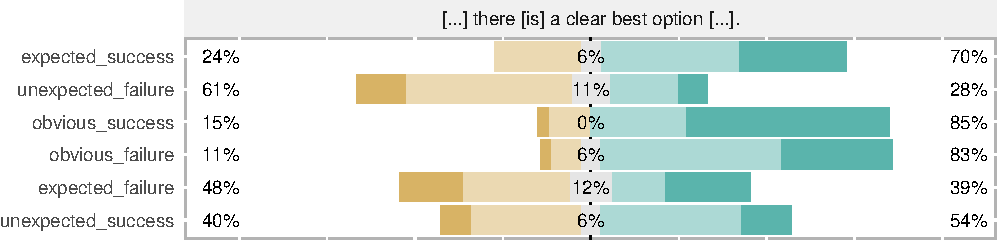
\includegraphics[width=\textwidth]{{fig/cropped-outcomes-report-01-opt.obvious}.pdf}
  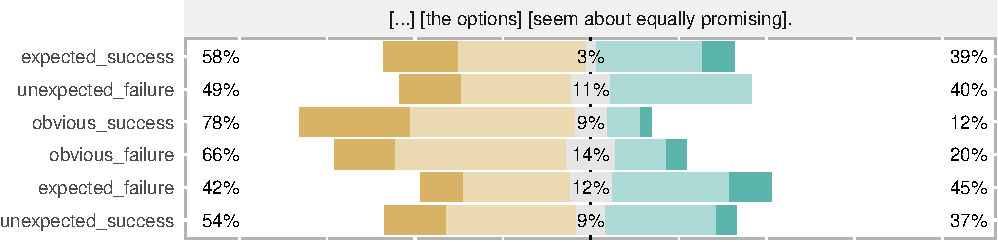
\includegraphics[width=\textwidth]{{fig/cropped-outcomes-report-02-opt.balanced}.pdf}
  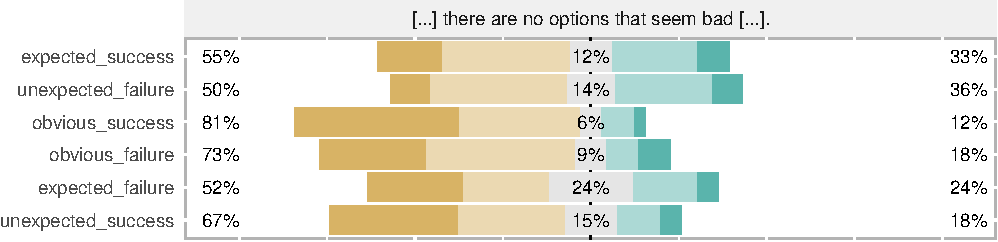
\includegraphics[width=\textwidth]{{fig/cropped-outcomes-report-03-opt.nobad}.pdf}
  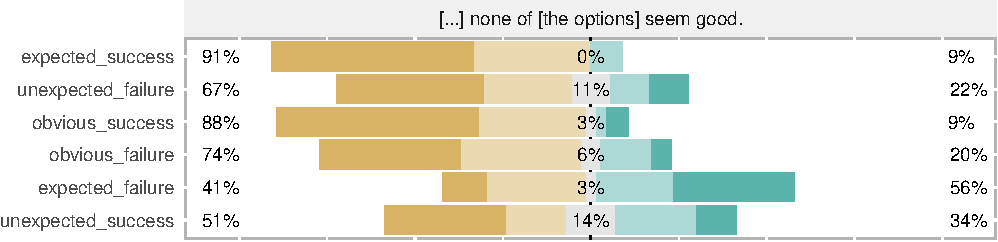
\includegraphics[width=\textwidth]{{fig/cropped-outcomes-report-04-opt.nogood}.pdf}
  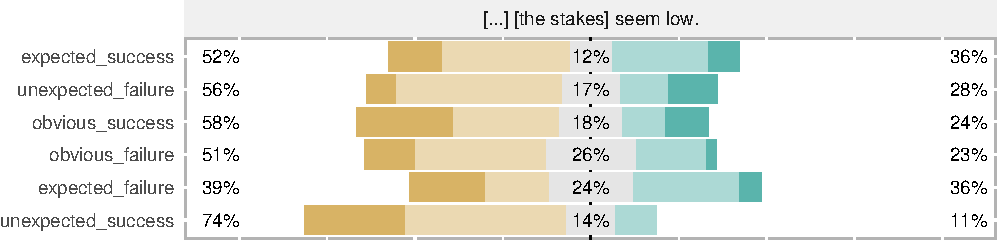
\includegraphics[width=\textwidth]{{fig/cropped-outcomes-report-05-opt.stakes}.pdf}
  
\includegraphics[width=\textwidth]{fig/outcomes-legend-custom.pdf}
  \caption[Retrospective option results]{Option-related results from the retrospective study. Cf. \cref{fig:e1-report}.}
  \label{fig:e2-option-report}
\end{figure}

\begin{figure}[!p]
  \centering
  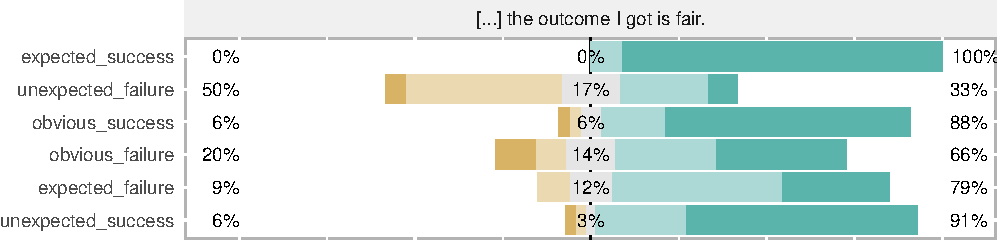
\includegraphics[width=\textwidth]{{fig/cropped-outcomes-report-10-out.fair}.pdf}
  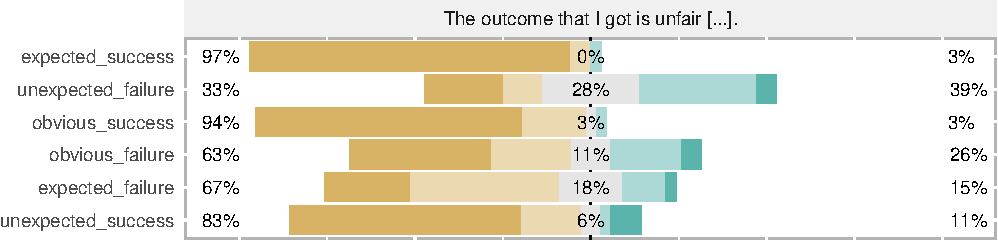
\includegraphics[width=\textwidth]{{fig/cropped-outcomes-report-11-out.unfair}.pdf}
  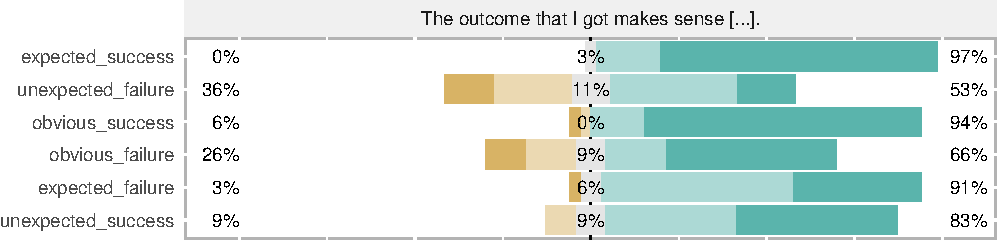
\includegraphics[width=\textwidth]{{fig/cropped-outcomes-report-12-out.sense}.pdf}
  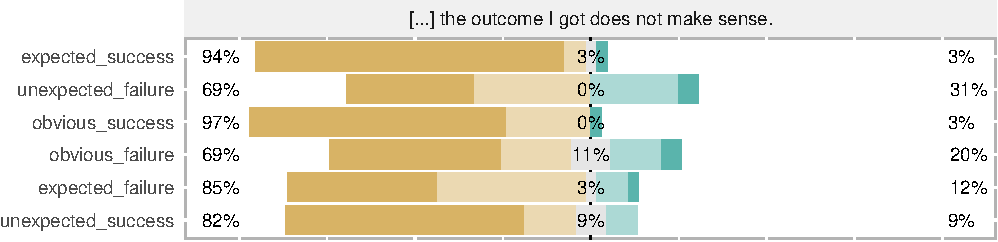
\includegraphics[width=\textwidth]{{fig/cropped-outcomes-report-13-out.broken}.pdf}
  
\includegraphics[width=\textwidth]{fig/outcomes-legend-custom.pdf}
  \caption[Retrospective fair/unfair \& sense/nonsense results]{Fair/unfair and sense/nonsense results from the retrospective study. Setup is the same as \cref{fig:e1-report}.}
  \label{fig:e2-outcome-report-fair-sense}
\end{figure}

\begin{figure}[!p]
  \centering
  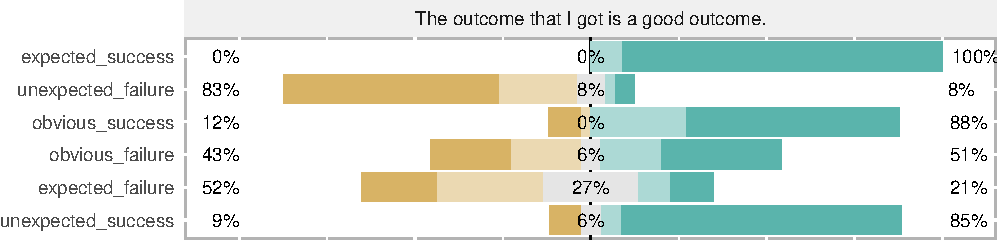
\includegraphics[width=\textwidth]{{fig/cropped-outcomes-report-06-out.good}.pdf}
  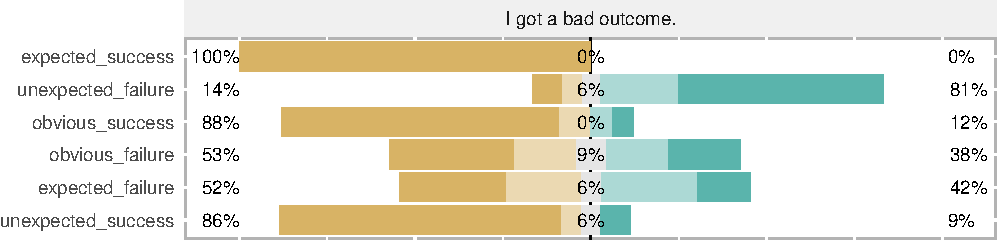
\includegraphics[width=\textwidth]{{fig/cropped-outcomes-report-07-out.bad}.pdf}
  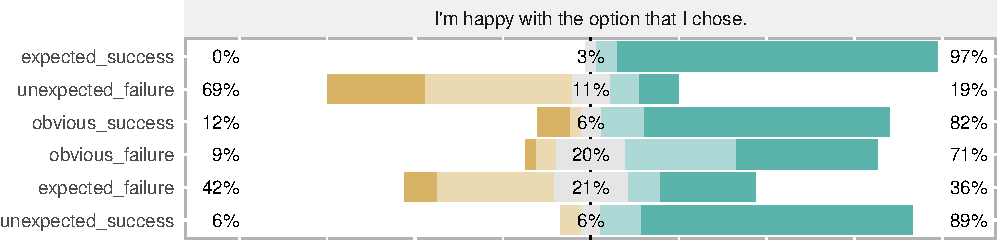
\includegraphics[width=\textwidth]{{fig/cropped-outcomes-report-14-out.happy}.pdf}
  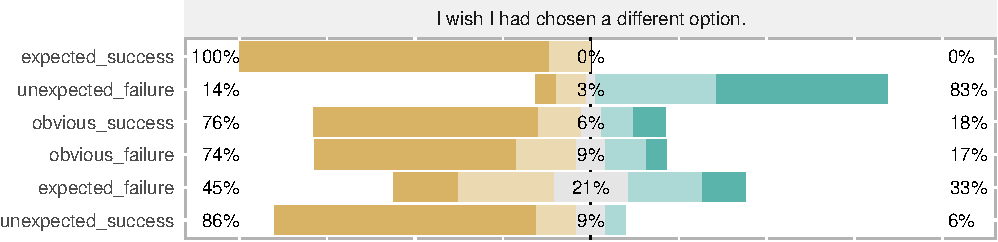
\includegraphics[width=\textwidth]{{fig/cropped-outcomes-report-15-out.regret}.pdf}
  
\includegraphics[width=\textwidth]{fig/outcomes-legend-custom.pdf}
  \caption[Retrospective good/bad \& satisfied/dissatisfied results]{Good/bad and satisfied/dissatisfied results from the retrospective study. Setup is the same as \cref{fig:e1-report}.}
  \label{fig:e2-outcome-report-valence-satisfaction}
\end{figure}

\begin{figure}[!t]
  \centering
  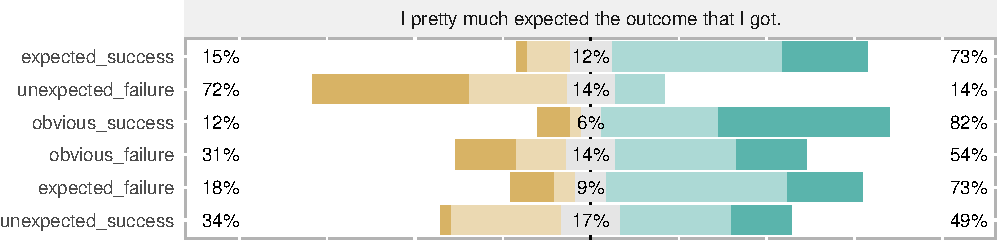
\includegraphics[width=\textwidth]{{fig/cropped-outcomes-report-08-out.expected}.pdf}
  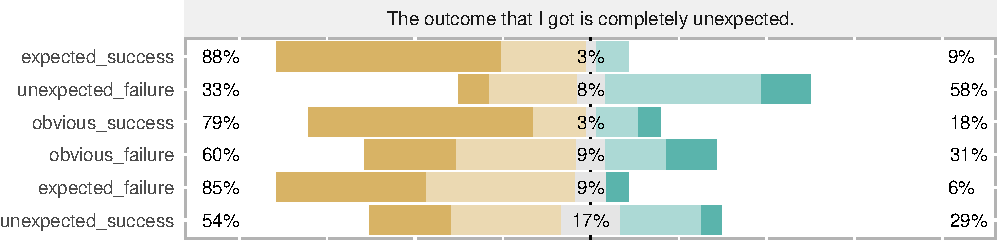
\includegraphics[width=\textwidth]{{fig/cropped-outcomes-report-09-out.unexpected}.pdf}
  
\includegraphics[width=\textwidth]{fig/outcomes-legend-custom.pdf}
  \caption[Retrospective expected/unexpected results]{Expected/unexpected retrospective results. Setup as in \cref{fig:e1-report}.}
  \label{fig:e2-outcome-report-surprise}
\end{figure}

\subsection{Summary}

A summary of the results appears in \cref{fig:e2-option-report,fig:e2-outcome-report-fair-sense,fig:e2-outcome-report-valence-satisfaction,fig:e2-outcome-report-surprise}, which have the same format as \cref{fig:e1-report}.
%
\Cref{fig:e2-option-report} includes all of the option-related questions, and can be compared directly to results in \cref{fig:e1-report}, especially for the last four conditions, which correspond in pairs to the \obv{} and \dlm{} conditions of the first experiment, respectively.
%
In \cref{fig:e2-outcome-report-fair-sense,fig:e2-outcome-report-valence-satisfaction,fig:e2-outcome-report-surprise}, the questions are ordered such that complimentary question pairs are adjacent, and comparing the data visually there seems to be a good deal of symmetry between these pairs, as expected.
%
Overall, the data indicate that \dunyazad/ is better at creating positive expectations and results than negative ones: compare the incredibly one-sided results for the \exps{} condition to the much more mixed results for \expf{,} for example.


As mentioned above, each of the rows in these figures represents between 32 and 36 responses, depending on the condition.
%
The sub-cases (e.g., \obvfm{} vs\@. \obvfa{}) are not separated here, although they are analyzed separately for some of the hypotheses.
%
For the \obvs{} condition, 25 of the 33 responses fell into the [main] sub-case, while the remaining 8 participants chose an option other than the one that \dunyazad/ expected would be most promising.
%
For the \obvf{} condition, the \casem{} sub-case contained 20 of the 35 responses, while the [alt] sub-case contained the remaining 15.
%
Note that each condition can be broken down into three individual choices, and there is a general expectation that these three choices will elicit generally similar responses, as they are constructed using the same set of constraints (although they are required to use three different setups).
%
Slight variation between choices within a condition should not disrupt the overall results, of course, but if there is significant divergence, it may be a sign that \dunyazad/'s internal reasoning about a choice doesn't agree with how participants experience that choice.


\section{Option Results}

\Cref{tab:e2-option-results} shows the results for the option-related hypotheses, with significant results listed in bold.
%
Note that in line with the results of the first study, none of the low-confidence hypotheses were supported by the data.
%
These hypotheses (marked with `\lc/') involved predictions which don't hold up if participants judge options relative to each other instead of in absolute terms, and the prospective study indicated strongly that this was the case for many participants.

\begin{table}[!t]
\centering
\bgroup
\def\arraystretch{1.3}
\setlength{\tabcolsep}{0.35em}
\begin{tabular}{r  c  c c c  c  c c c  c  c c c}
\toprule
\multirow{2}{5em}{\centering Question} &%
 & \multicolumn{3}{c}{\eIIexpectedsuccessabbr/} &%
 & \multicolumn{3}{c}{\eIIobvioussuccessabbr/} &%
 & \multicolumn{3}{c}{\eIIexpectedfailureabbr/} \\
&%
 & \multicolumn{3}{c}{\eIIunexpectedfailureabbr/} &%
 & \multicolumn{3}{c}{\eIIobviousfailureabbr/} &%
 & \multicolumn{3}{c}{\eIIunexpectedsuccessabbr/} \\
\midrule
\multirow{2}{5em}{\raggedleft \eIIoptobviousabbr/} &%
 & \tensig{D\lc/}{0.987} &%
 & \tesig{A}{$\bm{8.3\sqtimes 10^{-5}}$}{75\%} &%
 & \tensig{D\lc/}{0.467} \\
&%
 & \tensig{D\lc/}{0.128} &%
 & \tesig{A}{0.001}{70\%} &%
 & \tensig{D\lc/}{0.717} \\
\midrule
\multirow{2}{5em}{\raggedleft \eIIoptbalancedabbr/} &%
 & \tensig{A\lc/}{0.809} &%
 & \tesig{D}{0.003}{69\%} &%
 & \tensig{A\lc/}{0.485} \\
&%
 & \tensig{A\lc/}{0.767} &%
 & \tesig{D}{0.045}{61\%} &%
 & \tensig{A\lc/}{0.794} \\
\midrule
\multirow{2}{5em}{\raggedleft \eIIoptnobadabbr/} &%
 & \tensig{A\lc/}{0.807} &%
 & \tesig{D}{$\bm{4.5\sqtimes 10^{-4}}$}{72\%} &%
 & \tensig{D}{0.082} \\
&%
 & \tensig{A\lc/}{0.683} &%
 & \tesig{D}{0.013}{65\%} &%
 & \tesig{D}{0.011}{66\%} \\
\midrule
\multirow{2}{5em}{\raggedleft \eIIoptnogoodabbr/} &%
 & \tesig{D}{$\bm{1.1\sqtimes 10^{-5}}$}{78\%} &%
 & \tesig{D}{$\bm{4.1\sqtimes 10^{-5}}$}{76\%} &%
 & \tensig{A}{0.140} \\
&%
 & \tesig{D}{0.013}{65\%} &%
 & \tesig{D}{0.004}{68\%} &%
 & \tensig{A}{0.883} \\
\midrule
\multirow{2}{5em}{\raggedleft \eIIoptstakesabbr/} &%
 & \tensig{D}{0.279} &%
 & \tensig{D}{0.081} &%
 & \tensig{D}{0.310} \\
&%
 & \tensig{D}{0.257} &%
 & \tensig{D}{0.121} &%
 & \tesig{D}{0.003}{68\%} \\
\bottomrule
\end{tabular}

\egroup
\caption[Retrospective option results]{Option-related results in the retrospective experiment. Each row lists results for a single question; each column stacks results for two conditions (listed at the top) with identical \prq{option\_feel}{} constraints. Each entry indicates the hypothesis (`D' for `disagree' and `A' for `agree'), the $p$-value, and the common-language effect size for confirmed hypotheses (which are marked in bold instead of \nsighcolor/ where $p < 0.05$).}
  \label{tab:e2-option-results}
\end{table}


\subsection{Stakes}
One immediate pattern in these results is the lack of support for the ``low stakes'' hypotheses.
%
In the initial study, the hypothesis that choices which \dunyazad/ labelled as high-stakes would appear that way to participants was clearly confirmed by the data, with a $p$-value of 0.0011 and an effect size of 70\% (a strong effect).
%
In this study, every single choice was required to be high-stakes, but only in a single case (the \unxs{} condition) was the relevant hypothesis confirmed.
%
One reason why this might be the case is that in this study, \dunyazad/ was not allowed to control either the setup or the stakes of the choices, whereas in the initial study \dunyazad/ was free to control both.
%
The high-stakes choices in this study therefore necessarily included choices with \prq{market}{} setups, where it is impossible for \dunyazad/ to construct a scenario that directly threatens the player's character.
%
A breakdown of responses to the stakes question across all conditions by setup (\cref{fig:e2-stakes-by-setup}) seems to confirm that the \prq{market}{} setup is a problem: it elicits an even split between agree and disagree responses while the other two setups lean towards disagreeing.

To test this theory, I did a followup analysis with three hypotheses---each individual setup as a condition was hypothesized to elicit disagreement with the low stakes statement.
%
The results of this analysis confirmed my suspicions.
%
The test for the \prq{market}{} hypothesis does not reject the null hypothesis ($p = 0.502$), while the tests for the \prq{threatened\_innocents}{} and \prq{monster\_attack}{} hypotheses are confirmed ($p = 0.041$; effect size 60\% and $p = 0.0093$; effect size 64\% respectively).
%
Essentially, when \dunyazad/ creates choices without constraints regarding their stakes, the high-stakes choices that it does create are in fact perceived to be high-stakes by players.
%
However, when \dunyazad/ is specifically asked to create high-stakes choices using certain fixed setups, such as the \prq{market}{} setup, it doesn't manage to create choices that are convincingly high-stakes.
%
Whether this means that the perception of stakes has more to do with the setup text than the actual content of the options and/or outcomes is an open question that could be tested.

\begin{figure}[!t]
  \centering
  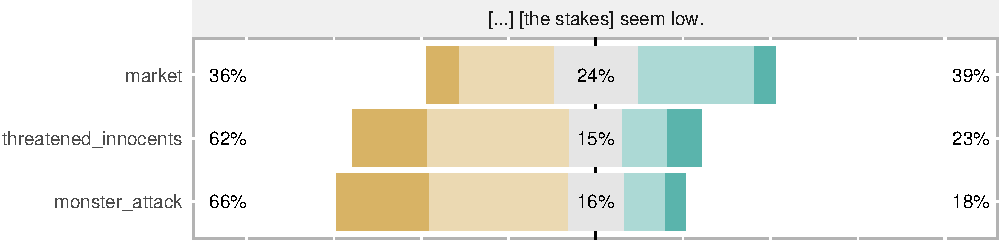
\includegraphics[width=\textwidth]{{fig/cropped-extra-outcomes-report-by-setup-05-opt.stakes}.pdf}\\
\hspace*{1.5pt}
\includegraphics[width=\textwidth]{fig/outcomes-legend-custom.pdf}
  \caption[Retrospective stakes results by setup]{Stakes results across all conditions grouped by the setup used.}
  \label{fig:e2-stakes-by-setup}
\end{figure}


\subsection{Expected Failure---No Bad Options?}

Besides the unconfirmed stakes hypotheses, there were two other places where high-confidence option-related hypothesis were not confirmed by the data.
%
The first is in the \expf{} case for the ``no bad'' statement.
%
Although the \unxs{} condition, which in theory generates options which set identical expectations, was confirmed to disagree with this statement, the data did not support this hypothesis for the \expf{} condition.
%
Of course, this condition is one susceptible to being undermined by relative value judgements: if all of the options seem bad, one might reason that it doesn't matter which is chosen, and therefore none of them are ``bad'' in the sense that choosing them would be a mistake.
%
It is telling that the \prq{obvious\_}{} cases confirmed corresponding hypotheses: when a single positive option was present alongside negative options, participants strongly rejected the notion that there were ``no bad options'' present.

\begin{figure}[!b]
  \centering
  {\sffamily Expected Failure}
  \includegraphics[width=\textwidth]{{fig/cropped-detailed-report-expected\string_failure-02-opt.nobad}.pdf}\\[1ex]
  {\sffamily Unexpected Success}
  \includegraphics[width=\textwidth]{{fig/cropped-detailed-report-unexpected\string_success-02-opt.nobad}.pdf}\\
  
\includegraphics[width=\textwidth]{fig/detailed-outcomes-legend-custom.pdf}
  \caption[Retrospective dilemma ``no bad options'' results]{Results for the ``no bad options'' statement in the \expf{} (top) and \unxs{} (bottom) conditions, grouped by choice. Each choice is identified by the numeric seed that was used to create it. The bracketed numbers on the right indicate the sample size for each choice.}
  \label{fig:e2-extra-nobad}
\end{figure}


But what about the difference between the \expf{} case and the \unxs{} case?
%
\Cref{fig:e2-extra-nobad} shows the results for each individual choice in both cases, and there isn't a clear culprit.
%
The choice with seed 58403 is the single choice among the six in that figure that elicited the most agreement with the statement, but it still tilts towards disagreement.
%
Given that both conditions include a substantial minority of ``agree'' and even ``strongly agree'' responses, there doesn't seem to be a clear underlying reason for the division in the results.
%
What is clear is that giving \dunyazad/ the ability to make relative rather than purely absolute value judgements should be a high priority.
%
In future studies, it might also be more productive to just ask participants to label each option as good/bad (and also suggests-success/suggests-failure), although as mentioned in the discussion of the setup for the first study, this kind of language promotes an analytical approach and that isn't necessarily desirable.


\begin{figure}[!b]
  \centering
  {\sffamily Expected Failure}
  \includegraphics[width=\textwidth]{{fig/cropped-detailed-report-expected\string_failure-03-opt.nogood}.pdf} \\[1ex]
  {\sffamily Unexpected Success}
  \includegraphics[width=\textwidth]{{fig/cropped-detailed-report-unexpected\string_success-03-opt.nogood}.pdf} \\
  
\includegraphics[width=\textwidth]{fig/detailed-outcomes-legend-custom.pdf}
  \caption[Retrospective dilemma ``no good options'' results]{Results for the ``no good options'' statement in the \expf{} (top) and \unxs{} (bottom) conditions, grouped by choice. The bracketed numbers in on the right indicate the sample size for each choice.}
  \label{fig:e2-extra-nogood}
\end{figure}


\subsection{Dilemma Cases---Competing Goals}
\label{sec:e2-competing-goals}

Another point of interest among the option-related results was the data's failure to support the hypotheses that the \expf{} and \unxs{} cases would be viewed as having ``no good options.''
%
Again, the \dlm{} case in the first experiment produced reactions that supported an equivalent hypothesis, so this result is somewhat surprising.
%
Here however the reasons for this discrepancy are clear.


\Cref{fig:e2-extra-nogood} shows the responses for these cases, and it is clear that the choices with seeds 87991, 8015, 47794, and 33152 are not yielding the expected results: participants are indicating that there is at least one good option at these choices.
%
\Cref{fig:e2-seed-87991} shows the choice with seed 87991, and the problem is immediately apparent: \dunyazad/ has used a \prq{travel\_onwards}{} action as a ``clearly bad result.''
%
This is a result of an overcorrection from the problems with \prq{travel\_onwards}{} that were discovered during the first study.
%
In that study, \prq{travel\_onwards}{} was a cure-all option which could get rid of any problem due to the way that it handled switching scenes.
%
For this second study, that bug was fixed, and instead, \prq{travel\_onwards}{} is marked as failing any goals relating to unresolved situations that it leaves behind. 
%
In this case, \dunyazad/ thinks that the  player will have an \prq{avoid\_accusations}{} goal with respect to the accused merchant, and simply leaving the merchant behind clearly fails this goal.

\begin{figure}[t]
\fseed{87991}
\caption[``Expected failure'' choice 87991]{The choice with seed 87991 minus the framing (which is mostly the same between choices). Boxed numbers before each outcome indicate the number of participants that chose that outcome. Note the popularity of the third option.}
\label{fig:e2-seed-87991}
\end{figure}


Of course, the underlying problem here is goal prioritization.
%
If given an good option to save the merchant, many players are eager to do so, but when such options are risky, they prefer to preserve their own safety.
%
With \dunyazad/'s two-level goal priority system, which was unchanged from the first experiment, it's not possible to represent this complexity.
%
Under the current system then, instead of \prq{travel\_onwards}{} being seen as an option with too few consequences, it is seen as an option with too many consequences.
%
The choice with seed 8015 also includes a \prq{travel\_onwards}{} option in a similar situation, and the inclusion of these options was likely the reason that players felt that the \expf{} cases actually \emph{did} have some good options.


\begin{figure}[h]
\fseed{47794}
\caption[``Unexpected success'' choice 47794]{The \unxs{} choice with seed 47794 minus its framing. Boxed numbers indicate the number of participants that selected each outcome.}
\label{fig:e2-seed-47794}
\end{figure}


\subsection{Dilemma Cases---Outcomes Affect Option Perception}

Recall that the \unxs{} case exhibited the same problem.
%
The reason for this was different, however, because neither the choice with seed 47794 nor the choice with seed 33152 had \prq{travel\_onwards}{} options.
%
Instead, the reason that these choices were rated as having at least one good option is probably their outcomes.
%
Because participants saw an outcome before answering any questions, the responses to the option questions could have been affected by the outcomes seen.
%
\Cref{fig:e2-seed-47794} shows the choice with seed 47794, and looking at it reveals a likely explanation for the ``no good options'' response.


As shown in that figure, six of ten participants who saw that choice chose the first option, and were ``unexpectedly'' successful.
%
But remember that \dunyazad/'s notion of what is expected is written in terms of system-wide rules: ``normally'' someone missing the negotiation skill should \emph{always} fail to talk someone else down, so if such an action succeeds the result is unexpected.
%
This kind of expectation is something that players would learn if they interacted with the system over a period of time, but participants in this study only saw a single choice.
%
Faced with a positive outcome, it would be natural to conclude that perhaps the negotiation skill isn't important after all, and therefore that the option that was chosen was a good one.
%
This line of reasoning would not be available to players before seeing an outcome, but as stated before, the risk of such influences was intentionally accepted as the price of a more natural decision-making experience.


Because the choice with seed 33152 included a very similar \prq{talk\_down}{} option which was also quite popular, this outcome-dependent effect can explain the failed hypothesis in the \unxs{} condition.
%
Unfortunately, the impact of this effect and the \prq{travel\_onwards}{} issue affecting the choices with seeds 87991 and 8015 is not negligible.
%
When it comes to evaluating the outcome-related hypotheses, these choices didn't convey the intended prospective poetics, and this could impact their retrospective poetics as well.


\subsection{Problems with \prq{travel\_onwards}{}}
\label{sec:e2-travel-onwards}

Besides choices in the two dilemma conditions, two other choices---the \obvs{} choices with seeds 47371 and 20739---also included \prq{travel\_onwards}{} options.
%
These are shown in \cref{fig:e2-seeds-47371-20739}.
%
Luckily, the choice with seed 47371 happens to give participants an option that's more attractive than the \prq{travel\_onwards}{} option, so the same problem doesn't occur.
%
In fact, this is a good example of correct use of \prq{travel\_onwards}{} as an option that seems bad, which is reinforced by the fact that zero participants chose it.
%
However, based on the option popularities in choice 20739, that choice has the same problems as choices 87991 and 8015: the ``correct'' option involves some perceived risk or cost (in this case giving away an item to resolve the situation) and so simply ignoring the merchant's plight is seen as acceptable.


\begin{figure}[p]
\fseed{47371} \\
\fseed{20739}
\caption[``Obvious success'' choices 47371 and 20739]{The \obvs{} choices 47371 and 20739 minus framing. Boxed numbers indicate the number of participants who saw each outcome.}
\label{fig:e2-seeds-47371-20739}
\end{figure}


Note that these options are in the \obvs{} condition, and as such participants who saw them are divided into the \prq{[main]}{} and \prq{[alt]}{} sub-cases according to which option they chose.
%
For choice 47371, all 11 participants who chose option two are in the \prq{[main]}{} sub-case, while the other two participants are in the \prq{[alt]}{} sub-case.
%
For choice 20739, there are only two participants that the system thinks chose the ``correct'' option, and the majority of participants are put into the \prq{[alt]}{} sub-case.
%
This means that the meaning of the sub-cases is somewhat changed from its intent.
%
The \prq{[alt]}{} cases are supposed to consist of participants who intentionally chose a non-positive option despite the presence of a positive one, and as such they are assumed to be quite small, to the point that not many hypotheses were proposed which included \prq{[alt]}{} cases.
%
Because of \dunyazad/'s failure to predict the complexities of player goals, the \prq{[alt]}{} case consists largely of participants who thought they were choosing the best option available, but who disagreed with \dunyazad/'s evaluation of what that was.
%
Of course, although these effects diminish the number of participants in the \prq{[main]}{} cases, at least their meaning is not diluted very much: only a few participants from poorly-formed choices like 20739 wound up choosing the options that \dunyazad/ considered best, and so only a few participants in the \prq{[main]}{} cases weren't choosing what they thought was an obviously superior option.


\subsection{Costly Actions}

One failure in \dunyazad/'s reasoning here, besides the inability to properly track goal priorities, is its focus on goals to the detriment of costs.
%
In other words, \dunyazad/ thinks about actions only in terms of the goals that they might achieve or threaten, and not in terms of the costs of those actions.
%
If the player must use an item to get what they want, \dunyazad/ neglects this cost and just sees that a goal is achieved.
%
Of course, this could be handled by adding player goals concerned with preserving resources, but the two-priority goal system doesn't leave room for such goals to affect high-stakes decisions even a little bit.

\begin{figure}[!b]
\fseed{95923}
\caption[``Obvious failure'' choice 95923]{The \obvf{} choice with seed 95923 minus framing. Boxed numbers indicate the number of participants that selected each outcome.}
\label{fig:e2-seed-95923}
\end{figure}


The choice with seed 20739 in \cref{fig:e2-seeds-47371-20739} is an example of this: In making a decision, even players who recognize that the first option will help the merchant have to somehow justify giving up their gold (and to a noble who doesn't deserve it, no less).
%
As the numbers indicate, most decided to simply travel onwards: the goal of helping the merchant was not worth the cost associated with it.
%
Of course, it doesn't help that the option text doesn't clearly state your intent in performing the action (to exonerate the merchant).\footnote{This issue has already been addressed by making the text more explicit for \prq{pay\_off}{} actions.}
%
In fact, one of the comments in the ``other'' free text response to the motivation question reveals exactly this kind of cost analysis in action:

\begin{quote}
  \quoteshape
You only really had 2 options. I wouldn't want to give up the gold if I didn't have to. So just negotiation made the most sense.
\end{quote}

This response was given by a participant who saw choice 95923, an \obvf{} choice shown in \cref{fig:e2-seed-95923}.
%
The fact that players are factoring costs into their decisions but \dunyazad/ is not tracking them is a problem.
%
Of course, the quote above reveals another problem: the choice with seed 95923 was supposed to be an \prq{obvious}{} choice with a single best option.
%
How did \dunyazad/ justify having two options that include positive skill indications?
%
In this case, \dunyazad/ has found what amounts to a loophole in its rules: the ``bad'' options at an obvious choice are allowed to be merely ``risky''---the reasoning is that compared to a really good option, a risky option will still be clearly inferior.
%
Because the \prq{talk\_down}{} action includes a risk that the target will begin accusing the initiator instead of their original victim, and because, internally, having the negotiation skill doesn't guarantee success, \dunyazad/ views the first option as a ``risky'' one: one that has an unsubstantiated benefit but also a potential drawback.
%
Three factors combined to throw off \dunyazad/'s analysis.
%
First, the unaccounted-for cost of the ``good'' option meant that it really wasn't as attractive as it should have been.
%
Second, the fact that talking the noble down carried a risk wasn't something that was made clear from the surface text.
%
Third, the fact that in the first option, \dunyazad/ does not count the negotiation skill as decisive while in the second option it does creates a false equivalence at the surface text level: both options appear equally supported by the ``negotiation'' skill.


This problem of costliness was specific to the \prq{pay\_off}{} action, which was present in the five choices with seeds 20739, 95923, 40550, 67832, and 82994.
%
Choice 20739 was just discussed in the context of the \prq{travel\_onwards}{} action and choice 95923 is the choice that prompted this analysis, but the other three choices have not yet been considered.
%
Luckily, choice 40550 was a \unxf{} choice and choices 67832 and 82994 were both \exps{} choices: all three were in conditions that were supposed to have three good options.
%
As a result, these costly options were presented along with two actually-good options, and in fact the costly options at these choices were chosen by one, zero, and zero participants respectively.
%
In other words, these options probably had little effect on the outcome-related results, as they were almost never chosen.
%
On the other hand, they do compromise the \emph{option} structures of the choices in question, and so they have a potentially important effect on the between-cases comparisons.


One good thing in all of this is that none of the factors that \dunyazad/ is currently neglecting are fundamentally difficult to account for.
%
For example, the fact that all 12 participants at choice 95923 chose the first option, which can be deduced to be the best using some simple extensions to \dunyazad/'s current logic, means that \dunyazad/'s general strategy of using \emph{character} motivations to predict \emph{player} actions is probably on the right track.
%
Extending \dunyazad/'s option evaluation code to reason about action costs, handle complex goal priorities, and reason about directly-presented implications rather than implications implied by hidden action logic may be technically challenging, but it's a clear set of features to implement.
%
Despite \dunyazad/'s failures, the results of this study strongly imply that with these features, \dunyazad/ will be able to correctly predict player's option evaluations most of the time.


\section{Outcome Results}

While the results of the option-related hypotheses were somewhat lackluster, this was to some degree expected based on the results of the first study.
%
Had more improvements been made to \dunyazad/ before the second study, this might have been avoided, but the primary purpose of this study was to evaluate \dunyazad/'s outcome predictions, which had not been tested by the first study.
%
\Cref{tab:e2-positive-outcome-results,tab:e2-negative-outcome-results} show the results for nominally-positive- and nominally-negative-outcome conditions respectively (the top and bottom halves of \cref{tab:e2-outcome-hypotheses}).
%
Overall, \dunyazad/ seems to be generally successful at producing positive outcomes, although it has some trouble making them surprising.
%
On the other hand, its track-record for negative outcomes is not as good.
%
In particular, surprising negative outcomes were more consistently rated as actually being ``bad,'' but participants didn't necessarily accept the idea that they were ``unfair'' or ``nonsense.''

\begin{table}[!p]
\centering
\bgroup
\def\arraystretch{1.2}
\setlength{\tabcolsep}{0.4em}
\begin{tabular}{r  c@{\hspace{2em}}  c c c  c@{\hspace{2em}} c c c}
\toprule
\multirow{2}{5em}{\centering Question} &%
 & \multicolumn{3}{c}{\eIIexpectedsuccessabbr/} &%
 & \multicolumn{3}{c}{\eIIunexpectedsuccessabbr/} \\
&%
 & \multicolumn{3}{c}{\eIIobvioussuccessmainabbr/} &%
 & \multicolumn{3}{c}{\eIIobviousfailurealtabbr/} \\
\midrule
\multirow{2}{6em}{\raggedleft \hangpara{1.3em}{1}\eIIoutfairabbr/} &%
 & \tesig{A}{$\bm{6.8\sqtimes 10^{-11}}$}{88\%} &%
 & \tesig{A}{$\bm{1.6\sqtimes 10^{-6}}$}{80\%} \\
&%
 & \tesig{A}{$\bm{1.7\sqtimes 10^{-8}}$}{87\%} &%
 & \tesig{A}{$\bm{1.1\sqtimes 10^{-5}}$}{85\%} \\
\midrule
\multirow{2}{6em}{\raggedleft \hangpara{1.3em}{1}\eIIoutunfairabbr/} &%
 & \tesig{D}{$\bm{2.7\sqtimes 10^{-10}}$}{87\%} &%
 & \tesig{D}{$\bm{3.5\sqtimes 10^{-5}}$}{76\%} \\
&%
 & \tesig{D}{$\bm{1.7\sqtimes 10^{-8}}$}{87\%} &%
 & \tesig{D}{$\bm{4.2\sqtimes 10^{-6}}$}{86\%} \\
\midrule
\multirow{2}{6em}{\raggedleft \hangpara{1.3em}{1}\eIIoutsenseabbr/} &%
 & \tesig{A}{$\bm{8.2\sqtimes 10^{-9}}$}{85\%} &%
 & \tesig{A}{$\bm{1.3\sqtimes 10^{-4}}$}{74\%} \\
&%
 & \tesig{A}{$\bm{4.7\sqtimes 10^{-8}}$}{85\%} &%
 & \tesig{A}{$\bm{4.2\sqtimes 10^{-6}}$}{86\%} \\
\midrule
\multirow{2}{6em}{\raggedleft \hangpara{1.3em}{1}\eIIoutbrokenabbr/} &%
 & \tesig{D}{$\bm{6.9\sqtimes 10^{-9}}$}{85\%} &%
 & \tesig{D}{$\bm{7.1\sqtimes 10^{-6}}$}{78\%} \\
&%
 & \tesig{D}{$\bm{1.7\sqtimes 10^{-6}}$}{82\%} &%
 & \tesig{D}{$\bm{1.1\sqtimes 10^{-5}}$}{85\%} \\
\midrule
\multirow{2}{6em}{\raggedleft \hangpara{1.3em}{1}\eIIoutgoodabbr/} &%
 & \tesig{A}{$\bm{6.8\sqtimes 10^{-11}}$}{88\%} &%
 & \tesig{A}{$\bm{1.5\sqtimes 10^{-6}}$}{79\%} \\
&%
 & \tesig{A}{$\bm{3.4\sqtimes 10^{-7}}$}{84\%} &%
 & \tesig{A}{$\bm{4.2\sqtimes 10^{-6}}$}{86\%} \\
\midrule
\multirow{2}{6em}{\raggedleft \hangpara{1.3em}{1}\eIIoutbadabbr/} &%
 & \tesig{D}{$\bm{6.7\sqtimes 10^{-13}}$}{90\%} &%
 & \tesig{D}{$\bm{9.2\sqtimes 10^{-7}}$}{80\%} \\
&%
 & \tesig{D}{$\bm{1.3\sqtimes 10^{-7}}$}{84\%} &%
 & \tesig{D}{$\bm{4.2\sqtimes 10^{-6}}$}{86\%} \\
\midrule
\multirow{2}{6em}{\raggedleft \hangpara{1.3em}{1}\eIIouthappyabbr/} &%
 & \tesig{A}{$\bm{1.7\sqtimes 10^{-10}}$}{88\%} &%
 & \tesig{A}{$\bm{1.4\sqtimes 10^{-7}}$}{82\%} \\
&%
 & \tesig{A}{$\bm{4.7\sqtimes 10^{-8}}$}{85\%} &%
 & \tesig{A}{$\bm{1.5\sqtimes 10^{-6}}$}{87\%} \\
\midrule
\multirow{2}{6em}{\raggedleft \hangpara{1.3em}{1}\eIIoutregretabbr/} &%
 & \tesig{D}{$\bm{2.2\sqtimes 10^{-10}}$}{88\%} &%
 & \tesig{D}{$\bm{4.8\sqtimes 10^{-7}}$}{81\%} \\
&%
 & \tesig{D}{$\bm{1.1\sqtimes 10^{-6}}$}{82\%} &%
 & \tesig{D}{$\bm{1.5\sqtimes 10^{-6}}$}{87\%} \\
\midrule
\multirow{2}{6em}{\raggedleft \hangpara{1.3em}{1}\eIIoutexpectedabbr/} &%
 & \tesig{A}{0.011}{66\%} &%
 & \tensig{D}{0.795} \\
&%
 & \tesig{A}{$\bm{3.0\sqtimes 10^{-4}}$}{75\%} &%
 & \tensig{D}{0.996} \\
\midrule
\multirow{2}{6em}{\raggedleft \hangpara{1.3em}{1}\eIIoutunexpectedabbr/} &%
 & \tesig{D}{$\bm{6.6\sqtimes 10^{-6}}$}{78\%} &%
 & \tensig{A}{0.896} \\
&%
 & \tesig{D}{$\bm{3.0\sqtimes 10^{-4}}$}{75\%} &%
 & \tensig{A}{0.997} \\
\bottomrule
\end{tabular}

\egroup
\caption[Retrospective positive outcome results]{The results from the retrospective study for conditions that have nominally positive outcomes. Each row stacks results from the two (sub-)conditions listed at the top. Each result lists the hypothesis (`A' for agree or `D' for disagree), the p-value, and if significant ($p < 0.05$) the common-language effect size.}
  \label{tab:e2-positive-outcome-results}
\end{table}

\begin{table}[!p]
\centering
\bgroup
\def\arraystretch{1.2}
\setlength{\tabcolsep}{0.4em}
\begin{tabular}{l  c  c c c  c  c c c}
\toprule
\multirow{2}{5em}{Question} &%
 & \multicolumn{3}{c}{Expected Failure} &%
 & \multicolumn{3}{c}{Unexp. Failure} \\
&%
 & \multicolumn{3}{c}{Obv. Success [alt]} &%
 & \multicolumn{3}{c}{Obv. Failure [main]} \\
\toprule
\midrule
\multirow{2}{8em}{\hangpara{1.3em}{1}\sIIoutfairabbr/} &%
 & \tesig{A}{0.001}{68\%} &%
 & \tensig{D}{0.343} \\
&%
 & \tensig{A}{0.274} &%
 & \tensig{D}{0.460} \\
\midrule
\multirow{2}{8em}{\hangpara{1.3em}{1}\sIIoutunfairabbr/} &%
 & \tesig{D}{0.017}{63\%} &%
 & \tensig{A}{0.634} \\
&%
 & \tesig{D}{0.024}{65\%} &%
 & \tensig{A}{0.419} \\
\midrule
\multirow{2}{8em}{\hangpara{1.3em}{1}\sIIoutsenseabbr/} &%
 & \tesig{A}{$\bm{1.2\sqtimes 10^{-4}}$}{72\%} &%
 & \tensig{D}{0.716} \\
&%
 & \tesig{A}{0.012}{67\%} &%
 & \tensig{D}{0.508} \\
\midrule
\multirow{2}{8em}{\hangpara{1.3em}{1}\sIIoutbrokenabbr/} &%
 & \tesig{D}{$\bm{4.2\sqtimes 10^{-4}}$}{70\%} &%
 & \tensig{A}{0.981} \\
&%
 & \tesig{D}{$\bm{6.2\sqtimes 10^{-4}}$}{74\%} &%
 & \tensig{A}{0.783} \\
\midrule
\multirow{2}{8em}{\hangpara{1.3em}{1}\sIIoutgoodabbr/} &%
 & \tensig{D}{0.129} &%
 & \tesig{D}{$\bm{2.6\sqtimes 10^{-5}}$}{73\%} \\
&%
 & \tensig{D}{0.519} &%
 & \tesig{D}{0.006}{67\%} \\
\midrule
\multirow{2}{8em}{\hangpara{1.3em}{1}\sIIoutbadabbr/} &%
 & \tensig{A}{0.762} &%
 & \tesig{A}{$\bm{1.7\sqtimes 10^{-4}}$}{71\%} \\
&%
 & \tensig{A}{0.919} &%
 & \tesig{A}{0.014}{65\%} \\
\midrule
\multirow{2}{8em}{\hangpara{1.3em}{1}\sIIouthappyabbr/} &%
 & \tenp  &%
 & \tesig{D}{0.024}{62\%} \\
&%
 & \tenp  &%
 & \tensig{D}{0.809} \\
\midrule
\multirow{2}{8em}{\hangpara{1.3em}{1}\sIIoutregretabbr/} &%
 & \tenp  &%
 & \tesig{A}{$\bm{3.7\sqtimes 10^{-4}}$}{70\%} \\
&%
 & \tenp  &%
 & \tensig{A}{0.897} \\
\midrule
\multirow{2}{8em}{\hangpara{1.3em}{1}\sIIoutexpectedabbr/} &%
 & \tesig{A}{0.031}{61\%} &%
 & \tesig{D}{$\bm{9.5\sqtimes 10^{-4}}$}{68\%} \\
&%
 & \tensig{A}{0.129} &%
 & \tensig{D}{0.168} \\
\midrule
\multirow{2}{8em}{\hangpara{1.3em}{1}\sIIoutunexpectedabbr/} &%
 & \tesig{D}{$\bm{2.9\sqtimes 10^{-4}}$}{70\%} &%
 & \tensig{A}{0.184} \\
&%
 & \tesig{D}{0.036}{64\%} &%
 & \tensig{A}{0.313} \\
\bottomrule
\end{tabular}

\egroup
\caption[Retrospective negative outcome results]{The results from the retrospective study for conditions that have nominally negative outcomes. The format is the same as that of \cref{tab:e2-positive-outcome-results}.}
\label{tab:e2-negative-outcome-results}
\end{table}


\subsection{Outcomes and Option Perception (Again)}

The only hypotheses regarding nominally successful outcomes that weren't confirmed were those regarding the expectedness of the nominally unexpected cases.
%
These two conditions, the \unxs{} and \obvfa{} conditions, were supposed to be cases where a participant chose an option which carried some indicator that it would fail, but got a successful result.
%
The choices involved had seeds 99500, 47794, and 33152 (\unxs{}); and 8638, 28306, and 95923 (\obvf{}).
%
Of course, only participants who didn't choose the nominally best option at choices 8638, 28306, and 95923 fell into the \obvfa{} case.


Unfortunately, the failure to confirm these hypotheses is not terribly surprising: out of all of the outcome-related statements, the statements about expectedness and unexpectedness are the most heavily dependent on participant's perception of the option text as opposed to only the outcome text.
%
Because several of the choices listed above had problems with option perceptions, they didn't really fit the outcome profile that the hypotheses were expecting.
%
Choices 47794 (see \cref{fig:e2-seed-47794}) and 33152 (not shown) together account or 24 of the 35 \unxs{} responses, and as already discussed, they each included a popular option that \emph{in light of its outcome} did not seem like a bad option.
%
Because the option text alone didn't give players a strong negative expectation for these options, positive results were not only not surprising; they made the option seem like it had been a good one from the start.


The fact that participants marked the outcomes of these options as expected might also point to a different effect: player trust in game-like systems.
%
In most modern games, unless the player has already received substantial warnings that they are on the wrong path, there won't be choices that have no ``correct'' option: even the worst situations will have some means of escape if the player is thrust into them without control over prior situations.
%
Because participants in this study only saw one choice, they may have assumed that there would be a ``correct'' option that would lead to a successful result.
%
With this expectation in mind, it's not surprising at all that choosing what one thinks is the best result will lead to a good outcome, even if the option text includes some negative indicator.


From the perspective of choice poetics, both of these possible effects are important to keep in mind.
%
First is the idea that options and outcomes both influence the perception of the other.
%
In this case, because \dunyazad/ did not make clearly bad-seeming options, a positive outcome was able to make those options seem like good options (at the very least, relative to other options at those choices).
%
Of course, given that those options seemed good, the notion that a good outcome would be surprising was no longer valid.
%
In other words, players reason neither strictly from options to outcomes nor from outcomes to options, but their perceptions of both affect their perceptions of the other.
%
If fact, there is ample evidence of this kind of reasoning even in real-world decisions (for an extreme example see studies on choice blindness such as \citep{Hall2012}).
%
If an author is interested in constructing an option that feels a specific way in retrospect, then, they must be mindful of the consequences of that option.


If the fact that options meant to seem indicative of failure were not explains the expectedness result in the \unxs{} case, what about the \obvfa{} case?
%
Choice 95923 from that case has already appeared here as well (see \cref{fig:e2-seed-95923}) and in combination with a graph of all responses to the ``expected'' question in \obvfa{} cases (\cref{fig:e2-obvious-failure-detail}) explains what is going on.
%
Essentially, \dunyazad/'s failure to make choice 95923 obvious flooded the \obvfa{} sub-case with 12 responses that dominated the three from the other two choices (which were clearly much better at getting participants to choose the intended choice).
%
The \obvfa{} sub-case therefore does not mainly consist of players who chose a bad option but got a good result.
%
Instead, it mainly consists of players who chose option one at choice 95923, which as already discussed, seemed to be a clearly positive option.
%
Because of this, getting a good result was not surprising, and the corresponding hypotheses were not confirmed.

\begin{figure}[!b]
  \centering
  {\sffamily Obvious Failure [alt]}
  \includegraphics[width=\textwidth]{{fig/cropped-detailed-report-obvious\string_failure(alt)-08-out.expected}.pdf}
  
\includegraphics[width=\textwidth]{fig/detailed-outcomes-legend-custom.pdf}
  \caption[Retrospective obvious failure ``expected'' results]{Results for the ``expected'' statement in the \obvfa{} sub-case, grouped by seed. Note the bracketed numbers on the right which indicate the sample size for each choice: seed 95923 dominates this category.}
  \label{fig:e2-obvious-failure-detail}
\end{figure}

\subsection{Outcome Text vs\@. States}

\begin{figure}[!p]
\centering%
\fseed{99500}\\[1ex]
{ \sffamily Unexpected Success}\\
\includegraphics[width=\textwidth]{{fig/cropped-detailed-report-unexpected\string_success-06-out.bad}.pdf}\\
\includegraphics[width=\textwidth]{{fig/cropped-detailed-report-unexpected\string_success-10-out.good}.pdf}\\

\includegraphics[width=\textwidth]{fig/detailed-outcomes-legend-custom.pdf}
\caption[``Unexpected success'' valence results and choice 99500]{The choice with seed 99500 along with valence results from the \unxs{} condition. Boxed values indicate the number of participants that selected each outcome at choice 99500, and bracketed numbers on the right of the graph below indicate sample sizes for each row. Note the diverging responses for choice 99500 and the text of the outcome for option one.}
\label{fig:e2-seed-99500-plus}
\end{figure}

Before moving on to discuss the nominally-negative outcome hypotheses, there's one more choice that didn't quite give expected results from the \unxs{} condition.
%
This is choice 99500 (shown in \cref{fig:e2-seed-99500-plus}), which stood out because a sizeable minority felt that the outcome they got was bad.
%
Inspecting the choice reveals the problem: the result of option one includes outcome text that seems at odds with itself: ``you are defeated,'' but the ogre is ``no longer threatening you'' and ``she is now injured.''
%
Within the system of outcome constraints placed on the \prq{attack}{} action, this is allowed: defeat of the target precludes the death of the attacker, but they may still be injured.
%
The real problem here is that the ``defeated'' outcome does not have any direct effects on the state of the world, unless the defeated party is threatening or accusing someone, in which case those states are removed.


Because \dunyazad/ generated a ``defeat'' with no negative consequences attached in terms of world state, it viewed that ``defeat'' as it would a victory: state changes effected by the action are unambiguously positive for the player, so the result is a ``success.''
%
Of course, participants felt otherwise: of the four participants that selected that option, three gave the anomalous responses to the valence questions shown in \cref{fig:e2-seed-99500-plus} and the fourth supplied both neutral responses.
%
The disconnect here between the text and \dunyazad/'s internal representation of the world causes a rift between its predictions and player's actual impressions.
%
Furthermore, one can question whether \dunyazad/ should be able to generate such a situation in the first place: shouldn't ``defeat'' come bundled with a negative consequence such as being at the mercy of the victor?
%
In this case, the effect was isolated enough that it didn't upset any hypotheses, but forcing a clear link between every outcome reflected in the text and a definite internal state would help avoid situations like this.


\subsection{The Outcome of \prq{travel\_onwards}{}}

\begin{figure}[t]
  \centering
  {\sffamily Expected Failure}\\
\includegraphics[width=\textwidth]{{fig/cropped-detailed-report-expected\string_failure-06-out.bad}.pdf}\\
\includegraphics[width=\textwidth]{{fig/cropped-detailed-report-expected\string_failure-10-out.good}.pdf}\\[1ex]
{\sffamily Obvious Success [alt]}\\
\includegraphics[width=\textwidth]{{fig/cropped-detailed-report-obvious\string_success(alt)-06-out.bad}.pdf}\\
\includegraphics[width=\textwidth]{{fig/cropped-detailed-report-obvious\string_success(alt)-10-out.good}.pdf}\\
\hspace*{2pt}
\includegraphics[width=\textwidth]{fig/detailed-outcomes-legend-custom.pdf}
\caption[``Expected failure'' valence results]{Results for the ``good'' and ``bad'' items from the \expf{} and \obvsa{} conditions. Bracketed numbers on the right indicate sample sizes for each row; note that the \obvsa{} condition is dominated by choice 20739, and even then has only 8 samples in total.}
\label{fig:e2-expected-failure-detail}
\end{figure}

As already mentioned, in its present state \dunyazad/ views \prq{travel\_onwards}{} actions as much more negative than participants, who often found simply ignoring a problem to be an acceptable choice.
%
This was not only true of option perceptions, but of outcome perceptions as well.
%
In fact, the failure of \expf{} and \obvsa{} choices to give reliably negative results (shown in \cref{tab:e2-negative-outcome-results}) can be attributed to this problem.
%
As shown in \cref{fig:e2-expected-failure-detail}, which graphs responses to the ``good'' and ``bad'' statements for the \expf{} and \obvsa{} conditions, the choices where a majority of participants felt that the outcome was positive are all choices containing \prq{travel\_onwards}{} options (choices 87991, 8015, and 20739, discussed above).
%
These \prq{travel\_onwards}{} options, which the system considers to be unambiguously bad (because the player's character fails to help someone in need), are seen by players as a good or at least mixed result: they have successfully avoided an otherwise troublesome situation.
%
The presence of these options neatly explains the left-hand column of \cref{tab:e2-negative-outcome-results}: they aren't viewed as bad, but they are seen as fair, sensible, and expected.
%
The only remaining unconfirmed hypotheses are those for the \obvsa{} sub-case, but those can also be explained with reference to \cref{fig:e2-expected-failure-detail}: the simple lack of data for the \casea{} sub-case of the \obvs{} condition (eight responses total) makes such hypotheses difficult to confirm statistically.
%
The fact that the bulk of the \obvsa{} case responses (5) were from participants who selected to \prq{travel\_onwards}{} at choice 20739 (cf. \cref{fig:e2-seeds-47371-20739}) didn't help matters.

\begin{figure}[p]
  \centering
  {\sffamily Unexpected Failure}\\
\includegraphics[width=\textwidth]{{fig/cropped-detailed-report-unexpected\string_failure-09-out.fair}.pdf}\\
\includegraphics[width=\textwidth]{{fig/cropped-detailed-report-unexpected\string_failure-15-out.unfair}.pdf}\\
\includegraphics[width=\textwidth]{{fig/cropped-detailed-report-unexpected\string_failure-13-out.sense}.pdf}\\
\includegraphics[width=\textwidth]{{fig/cropped-detailed-report-unexpected\string_failure-07-out.broken}.pdf}
{\sffamily Obvious Failure [main]}\\
\includegraphics[width=\textwidth]{{fig/cropped-detailed-report-obvious\string_failure(main)-09-out.fair}.pdf}\\
\includegraphics[width=\textwidth]{{fig/cropped-detailed-report-obvious\string_failure(main)-15-out.unfair}.pdf}\\
\includegraphics[width=\textwidth]{{fig/cropped-detailed-report-obvious\string_failure(main)-13-out.sense}.pdf}\\
\includegraphics[width=\textwidth]{{fig/cropped-detailed-report-obvious\string_failure(main)-07-out.broken}.pdf}
\caption[Unexpected failure fairness and sense results]{Results for the fairness and sense items in the \unxf{} and \obvfm{} conditions. Bracketed numbers on the right indicate sample sizes for each row. Scale as per previous figures.}
\label{fig:e2-unexpected-failure-detail-fair-sense}
\end{figure}


\subsection{Fairness and The Strength of Expectations}

Examining the \emph{unexpected} failure conditions (the right half of \cref{tab:e2-negative-outcome-results}) it is immediately apparent that participants found them to be more fair and less broken than expected.
%
The relevant rows of \cref{fig:e2-outcome-report-fair-sense} indicate that these two conditions did stand out as the \emph{least} fair and \emph{most} broken cases, but they were not found to be more unfair than fair or more broken than sensible, as expected.
%
\Cref{fig:e2-unexpected-failure-detail-fair-sense} breaks down the responses by individual choice, and gives a sense as to which choices were viewed as more fair (and/or less broken) than others.
%
In the \unxf{} condition, the choice with seed 46585 stands out as seeming more fair than its companions, and in the \obvfm{} condition, the choice with seed 28306 seems to be the culprit.


\begin{figure}[!b]
\fseed{46585}
\caption[``Unexpected failure'' choice 46585]{The \unxf{} choice with seed 46585. Boxed numbers indicate the number of participants who selected each outcome.}
\label{fig:e2-seed-46585}
\end{figure}


\Cref{fig:e2-seed-46585,fig:e2-seed-28306} display the choices in question, and they share a common property that's likely related to why they were seen as fair: despite their differing option structures, they include options which generate only weak expectations of success, and which have somewhat mixed results.
%
In choice 46585, both the first and third options involve some kind of debate, and while the ``negotiation'' skill probably helps debate successfully, it's not the kind of action where the result would ever be a forgone conclusion.
%
The same is true in choice 28306: the attack option involves fighting, which is an action often prone to unexpected results, and furthermore, the advantage ascribed to the player in the option text is only marginal: possession of a weapon when both parties have the relevant skill.

\begin{figure}[t]
\fseed{28306}
\caption[``Obvious failure'' choice 28306]{The \obvf{} choice with seed 28306. Boxed numbers indicate the number of participants who selected each outcome.}
\label{fig:e2-seed-28306}
\end{figure}


Besides the fact that these choices don't set up strong expectations with their option text, they also don't have unreservedly negative results.
%
For example, in the third outcome of choice 46585, while it's true that failing to get rid of an accusation as intended is a bad thing, it's not necessarily awful: maybe the player will get another chance to address the situation before something really bad happens.
%
Similarly in outcome three of choice 28306, despite sustaining an injury the overall battle ends in a draw (which the player might further perceive as ending the ogre's threat, although in the system's representation of the world the threat persists).
%
While these \emph{are} negative outcomes (and the results for the statement ``I got a bad outcome'' show that most participants agreed on this), are they negative enough to be considered ``unfair'' with respect to the expectations set up by the option text?
%
The subjects in the study didn't think so, and thus the hypotheses that these conditions would be perceived as unfair and possibly broken were not supported.

\begin{figure}[!t]
\fseed{8638}
\caption[``Obvious failure'' choice 8638]{The \obvf{} choice with seed 8638. Boxed numbers indicate the number of participants who selected each outcome. This is an example of \dunyazad/ successfully creating a choice that participants viewed as unfair.}
\label{fig:e2-seed-8638}
\end{figure}


In \dunyazad/'s internal calculus, these options all simply ``suggest success,'' and ``result in failure'' but evaluating them in human terms shows that the expectations that they set up are limited.
%
The contrast between these options and ones which players overwhelmingly found to be unfair (such as option two of choice 8638, shown in \cref{fig:e2-seed-8638}) is illustrative.
%
Choice 8638 combines an obvious option structure (so players feel they are making the correct decision by picking option two) with a disappointing failure.
%
The desire to see the results of the polymorph spell might have something to do with the strong reactions to choice 8638, but the fact that the option text of option two mentions two positive factors and no negative ones is likely important as well.
%
If an author is intentionally trying to create a choice that is perceived as unfair, it seems that being subtle when suggesting a positive outcome is a dangerous approach.


\subsection{Regret and Alternatives}
\label{sec:results-about-regret}

Another unexpected result in the unexpected failure column was the fact that participants weren't dissatisfied with their decisions at \obvf{} choices.
%
In retrospect, these hypotheses were poorly thought out: the \obvfm{} case should be one in which a participant selects what appears to be the only available good option, but is given a negative outcome.
%
Although one would expect such outcomes to be perceived as bad (which they were), the questions about satisfaction were asking whether participants \emph{would rather have picked a different option.}
%
If a participant truly thinks that the option they picked is the only good option, then despite a negative result, they should not believe that picking a different option would lead to a better outcome.
%
Of course, it's not the case that they clearly \emph{wouldn't} want to try a different option---the outcome they got \emph{was} bad---so neither enthusiastic agreement nor firm denial seem like appropriate responses.


The answers that I got reflected these competing impulses: the ``satisfied'' and ``dissatisfied'' statements both received a substantial number of neutral responses in the \obvfm{} condition, and the non-neutral responses were about evenly split overall, as shown in \cref{fig:e2-obvious-failure-main-detail-regret-expected}.
%
\Cref{fig:e2-seed-8638,fig:e2-seed-28306} (just shown) show the two choices that had any \casem{} responses in the \obvf{} condition; the data in \cref{fig:e2-obvious-failure-main-detail-regret-expected} all comes from the 20 participants who chose the most popular options at one of those choices.
%
While both choices are split, choice 28306 leans a bit more towards satisfaction, which may reflect being perceived as more fair, as just discussed.
%
Ultimately, the hypotheses that the \obvfm{} case would leave players feeling dissatisfied with their choice was shortsighted, and the mixed results that I got should have been expected given the tension between a bad result and a lack of viable alternatives produced by these choices.


\subsection{Expectations and... Expectedness}

The differences between choices 8638 and 28306 in terms of perceived fairness, brokenness, and satisfaction have been discussed, but there is one more pair of hypotheses relating to these choices that was not confirmed: the hypotheses stating that their results would be unexpected.
%
However, the issue of their differing expectations has already been discussed in relation to perceptions of fairness.
%
If choice 28306 is perceived as more fair because it gives rise to weaker expectations of success, then its negative result should be less unexpected than that of choice 8638.
%
Looking at the bottom two graphs in \cref{fig:e2-obvious-failure-main-detail-regret-expected}, this is exactly what was observed.

\begin{figure}[!p]
  \centering
{\sffamily Obvious Failure [main]}\\
\includegraphics[width=\textwidth]{{fig/cropped-detailed-report-obvious\string_failure(main)-11-out.happy}.pdf}\\
\includegraphics[width=\textwidth]{{fig/cropped-detailed-report-obvious\string_failure(main)-12-out.regret}.pdf}\\
\includegraphics[width=\textwidth]{{fig/cropped-detailed-report-obvious\string_failure(main)-08-out.expected}.pdf}\\
\includegraphics[width=\textwidth]{{fig/cropped-detailed-report-obvious\string_failure(main)-14-out.unexpected}.pdf}\\
\includegraphics[width=\textwidth]{fig/detailed-outcomes-legend-custom.pdf}
\caption[Obvious failure (main) regret and expectedness results]{Satisfaction and expectedness in the \obvfm{} condition. Bracketed numbers on the right indicate sample sizes for each row.}
\label{fig:e2-obvious-failure-main-detail-regret-expected}
\end{figure}


\begin{figure}[!p]
  \centering
{\sffamily Unexpected Failure}\\
\includegraphics[width=\textwidth]{{fig/cropped-detailed-report-unexpected\string_failure-08-out.expected}.pdf}\\
\includegraphics[width=\textwidth]{{fig/cropped-detailed-report-unexpected\string_failure-14-out.unexpected}.pdf}\\
\includegraphics[width=\textwidth]{fig/detailed-outcomes-legend-custom.pdf}
\caption[Unexpected failure expectedness results]{Results for the expectedness items in the \unxf{} condition. Bracketed numbers on the right indicate sample sizes for each row.}
\label{fig:e2-unexpected-failure-detail-unexpected}
\end{figure}


The weak positive expectations in choice 28306 are thus largely responsible for the failure of the \obvfm{} sub-case's results to be viewed as unexpected.
%
Of course, another factor was the makeup of choice 95923, the third \obvf{} choice, which did not contribute any samples to the \casem{} case.
%
If just choice 8638 is considered, the hypotheses that its outcome was unexpected are confirmed ($p=0.01337$, effect size 72\% for the ``not expected'' hypothesis and $p=0.014$, effect size 72\% for the ``was unexpected'' hypothesis) even with only 11 samples (including the non-\casem{} sample).
%
Had all three choices in the \obv{} condition produced results like choice 8638 (both in terms of participants choosing the expected option and the reactions to survey statements) the hypothesis that these types of outcomes were unexpected would have been confirmed.


The final unconfirmed hypothesis from the unexpected negative outcome column was that the \unxf{} condition would produce unexpected results.
%
The full hypothesis is actually half-confirmed, because participants did significantly disagree that the results were \emph{expected}, but they didn't agree that they were \emph{unexpected}.
%
\Cref{fig:e2-unexpected-failure-detail-unexpected} shows the results for both items in this condition, and it implicates choice 46585 as the culprit.
%
This choice was already discussed in the context of weak expectations, and is shown in \cref{fig:e2-seed-46585}.
%
That context is not a coincidence: the fact that the actions that it involves are inherently open-ended means that participants choose them with some doubt in their minds.
%
The difference between the positive and double-negative cases here is likely due to the outcomes at choice 46585 being neither expected nor unexpected.
%
Falling somewhere in between, they elicited disagreement with both the statement that they were ``pretty much expected'' and the statement that they were ``completely unexpected,'' thus helping confirm the positive hypothesis while working against the double negative hypothesis.


\section{Comparative Results}

There is much more to be said about the results of the outcome hypotheses and \dunyazad/'s overall performance (see \cref{sec:e2-discussion}), but first, it is useful to examine the results for the between-condition hypotheses.
%
These hypotheses were grouped into five topics which each probed for evidence of a different proposed effect, as discussed in \cref{sec:e2-relative-outcome-hypotheses}.

\subsection{Free vs\@. Forced Unexpected Failure}

The first such group predicted broadly that unexpected failure would be perceived as more acceptable when it seemed to be the result of a free choice rather than a forced one.
%
Stated another way, participants who experienced an unexpected failure at a choice where all options seemed good would be more likely to blame themselves for picking a ``wrong'' choice, and participants who picked an option that seemed to be clearly better than the alternatives would blame the system, accusing it of being unfair or broken and generally viewing their lot as worse.

\begin{table}[!p]
\centering
\bgroup
\def\arraystretch{1.3}
\setlength{\tabcolsep}{0.6em}
\begin{tabular}{l c c c}
\toprule
Question & Hypothesis & $p$-value & Effect \\
\midrule
\sIIoutfairabbr/ & \tensig{unexp. failure$>$obv. failure [main]}{0.640} \\
\sIIoutunfairabbr/ & \tensig{unexp. failure$<$obv. failure [main]}{0.292} \\
\sIIoutsenseabbr/ & \tensig{unexp. failure$>$obv. failure [main]}{0.339} \\
\sIIoutbrokenabbr/ & \tensig{unexp. failure$<$obv. failure [main]}{0.164} \\
\sIIoutgoodabbr/ & \tensig{unexp. failure$>$obv. failure [main]}{0.916} \\
\sIIoutbadabbr/ & \tensig{unexp. failure$<$obv. failure [main]}{0.902} \\
\sIIouthappyabbr/ & \tesig{unexp. failure$<$obv. failure [main]}{$\bm{7.7\sqtimes 10^{-4}}$}{71\%} \\
\sIIoutregretabbr/ & \tesig{unexp. failure$>$obv. failure [main]}{$\bm{3.7\sqtimes 10^{-5}}$}{76\%} \\
\sIIoutexpectedabbr/ & \tensig{unexp. failure$>$obv. failure [main]}{0.945} \\
\sIIoutunexpectedabbr/ & \tensig{unexp. failure$<$obv. failure [main]}{0.539} \\
\bottomrule
\end{tabular}
 \\[3ex]
\begin{tabular}{r c c c}
\toprule
Question & Hypothesis & $p$-value & Effect \\
\midrule
\eIIoutfairabbr/ & \tensig{unexp. failure$>$8638 [main]}{0.116} \\
\eIIoutunfairabbr/ & \tensig{unexp. failure$<$8638 [main]}{0.233} \\
\eIIoutsenseabbr/ & \tesig{unexp. failure$>$8638 [main]}{0.004}{77\%} \\
\eIIoutbrokenabbr/ & \tesig{unexp. failure$<$8638 [main]}{0.005}{76\%} \\
\eIIoutgoodabbr/ & \tensig{unexp. failure$>$8638 [main]}{0.305} \\
\eIIoutbadabbr/ & \tensig{unexp. failure$<$8638 [main]}{0.606} \\
\eIIouthappyabbr/ & \tesig{unexp. failure$<$8638 [main]}{0.004}{76\%} \\
\eIIoutregretabbr/ & \tesig{unexp. failure$>$8638 [main]}{$\bm{7.9\sqtimes 10^{-4}}$}{81\%} \\
\eIIoutexpectedabbr/ & \tensig{unexp. failure$>$8638 [main]}{0.296} \\
\eIIoutunexpectedabbr/ & \tesig{unexp. failure$<$8638 [main]}{0.018}{71\%} \\
\bottomrule
\end{tabular}

\egroup
\caption[Retrospective free vs\@. forced failure results]{%
Retrospective hypotheses for the claim that ``Unexpected failure is more acceptable when it happens at a freely-chosen option than when the player feels there are no viable alternative options.''
%
The bottom half shows the results when choice 8638 is allowed to stand in for the entire \obvfm{} case.
%
Each line lists the hypothesis, the $p$-value, and if significant ($p < 0.05$), the common-language effect size.
%
Low-confidence hypotheses are marked with a `\lc/'.
%
Note that each pair of rows contains opposing predictions, because complementary questions are arranged together.}
  \label{tab:e2-free-vs-forced-failure-results}
\end{table}


The results for the 10 individual hypotheses underlying this prediction are shown in the top half of \cref{tab:e2-free-vs-forced-failure-results}.
%
Unfortunately, all but two of them were not confirmed (and ironically, the two that were confirmed were ``low-confidence'' hypotheses).
%
Despite these results, the two confirmed hypotheses show extremely strong effects, and can be taken to indicate that a subset of the originally proposed effect is at work here.
%
Forced-choice unexpected failures may not be seen as more fair, less broken, better, or more expected than free-choice unexpected failures, but participants are definitely more-satisfied with their decisions in the forced-choice case.


Part of the reason that these hypotheses were mostly unsupported is that the choices in question didn't confirm the basic hypotheses about whether participants would agree or disagree with most of these questions (the two cases being compared here make up the right-hand column in \cref{tab:e2-negative-outcome-results}).
%
Only the valence and satisfaction statement hypotheses were confirmed as a pair for either of these cases, and the hypotheses for the satisfaction statements were only confirmed for the \unxf{} case.
%
As discussed above, the reasons for this have a lot to do with the general failure of the \obvfm{} case to live up to its name.
%
Because of the not-so-bad outcomes in the \obvfm{} case, not to mention the complications that the \unxf{} case had, the comparison between the \unxf{} and \obvfm{} cases isn't really testing what these hypotheses assumed it would be.


Comparing the \unxf{} case against just the most emblematic choice from the \obvfm{} case (choice 8638) gives a slightly different results, shown in the bottom half of \cref{tab:e2-free-vs-forced-failure-results}.
%
We can see that the prediction about fairness was not supported (although it wasn't firmly rejected either), but the prediction about sense/nonsense holds up.
%
The valence prediction is still unsupported, and the expectedness hypotheses are split, but overall it seems that the original idea wasn't wrong, but just overly broad.
%
Although more data would be needed to pin down this effect, it seems clear that the perception of alternatives to a chosen option as viable or not has an effect on how surprising negative outcomes are perceived.
%
If options perceived as viable alternatives are available, players will be both less satisfied with their decision (unsurprisingly) but they will also be more likely to label the result as one that makes sense, and less likely to label it as surprising (though not more likely to label it as expected).


\subsection{Chosen vs\@. Inevitable Success}

\begin{table}[!p]
\centering
\bgroup
\def\arraystretch{1.3}
\setlength{\tabcolsep}{0.6em}
\begin{tabular}{l c c c}
\toprule
Question & Hypothesis & $p$-value & Effect \\
\midrule
\sIIoutgoodabbr/ & \tensig{exp. success$<$obv. success [main]}{0.942} \\
\sIIoutbadabbr/ & \tensig{exp. success$>$obv. success [main]}{1.000} \\
\sIIouthappyabbr/ & \tensig{exp. success$<$obv. success [main]}{0.725} \\
\sIIoutregretabbr/ & \tensig{exp. success$>$obv. success [main]}{0.791} \\
\bottomrule
\end{tabular}

\egroup
\caption[Retrospective chosen vs\@. inevitable success results]{Retrospective between-conditions hypotheses concerning differences between expected successful outcomes in cases where the alternative options are either both positive or both negative.}
  \label{tab:e2-chosen-vs-inevitable-success-results}
\end{table}

\begin{figure}[!p]
  \centering
{\sffamily Expected Success}\\
\includegraphics[width=\textwidth]{{fig/cropped-detailed-report-expected\string_success-10-out.good}.pdf}\\
\includegraphics[width=\textwidth]{{fig/cropped-detailed-report-expected\string_success-11-out.happy}.pdf}\\
{\sffamily Obvious Success [main]}\\
\includegraphics[width=\textwidth]{{fig/cropped-detailed-report-obvious\string_success(main)-10-out.good}.pdf}\\
\includegraphics[width=\textwidth]{{fig/cropped-detailed-report-obvious\string_success(main)-11-out.happy}.pdf}\\
\includegraphics[width=\textwidth]{fig/detailed-outcomes-legend-custom.pdf}
\caption[Retrospective chosen vs\@. inevitable data summary]{Summary of the data in the \exps{} and \obvsm{} conditions for the ``good'' and ``satisfied'' items. The ``bad'' and ``dissatisfied'' items are not show but are similarly one-sided in the opposite direction. The last rows in the \obvsm{} case are negligible as they contain only 2 of the 25 samples in each plot (the problems with choice 20739 were discussed earlier).}
\label{fig:e2-chosen-vs-inevitable-success-detail}
\end{figure}

A second proposed between-conditions effect was that cases where success seemed to be the result of choosing a correct option would seem to have \emph{better} outcomes than cases where every option seemed likely to be successful, although both conditions were expected to be rated as generally good.
%
This proposed effect extended to the satisfied/dissatisfied items as well, but the results of testing these hypotheses, shown in \cref{tab:e2-chosen-vs-inevitable-success-results}, fail to support this claim.
%
A look at the distribution of responses to these questions, shown in \cref{fig:e2-chosen-vs-inevitable-success-detail}, reveals one possible reason for this: the results are simply oversaturated.


With the data I collected, the proposed subtle differences could have shown up as a shift from ``somewhat agree'' to ``strongly agree'' between the \exps{} and \obvsm{} conditions, but it turned out that even in the \exps{} condition, which I predicted to score lower, the responses were overwhelmingly\footnote{%
Note that although the responses to choice 20739 stand out, they represent only 2 of 25 samples in the \obvsm{} case, and thus don't have a meaningful effect on the statistics of these hypotheses.
%
The problems with choice 20739 (a costly choice paired off against a \prq{travel\_onwards}{} choice) have already been discussed.%
}\hspace{0.1em} ``strongly agree.''
%
To get data that might show such an effect, one approach would be to run a study using a 7- or 9-point Likert scale and hope that variation showed up in the upper regions of the scale.
%
Another approach would be to ask participants to directly rate \emph{how} good or satisfied they were, and provide response scales that included gradations of ``good'' such as ``good---great---excellent.''


\begin{table}[!t]
\centering
\bgroup
\def\arraystretch{1.3}
\setlength{\tabcolsep}{0.6em}
\begin{tabular}{r c c c}
\toprule
Question & Hypothesis & $p$-value & Effect \\
\midrule
\eIIoutfairabbr/ & \tesig{unexp. failure$<$unexp. success}{$\bm{4.5\sqtimes 10^{-9}}$}{86\%} \\
\eIIoutunfairabbr/ & \tesig{unexp. failure$>$unexp. success}{$\bm{5.7\sqtimes 10^{-5}}$}{75\%} \\
\eIIoutsenseabbr/ & \tesig{unexp. failure$<$unexp. success}{$\bm{3.7\sqtimes 10^{-4}}$}{72\%} \\
\eIIoutbrokenabbr/ & \tesig{unexp. failure$>$unexp. success}{0.004}{67\%} \\
\bottomrule
\end{tabular}

\egroup
\caption[Retrospective good vs\@. bad unexpected results]{Results for hypotheses asserting that unexpected positive outcomes will be perceived as more fair and less broken than unexpected negative outcomes.}
  \label{tab:e2-good-vs-bad-unexpected-results}
\end{table}

\subsection{Good vs\@. Bad Unexpected Results}

\Cref{tab:e2-good-vs-bad-unexpected-results} shows the results for another proposed effect: that unexpected good results would be seen as more fair and less broken than unexpected bad results.
%
In other words, when a result is the opposite of what is suggested by option text, if it's a good result players will tend to accept it, but if it's a bad result, they will tend to protest.
%
This is not a controversial hypothesis, and it was confirmed on all counts by the data.
%
An interesting followup would be to attempt to assess whether gradations of better and worse results have a linear effect on perceptions of fairness and sense or whether there is some kind of inflection point between the extremes used in this study.


\subsection{Expected vs\@. Unexpected Failures}

\begin{table}[!b]
\centering
\bgroup
\def\arraystretch{1.3}
\setlength{\tabcolsep}{0.6em}
\begin{tabular}{l c c c}
\toprule
Question & Hypothesis & $p$-value & Effect \\
\midrule
\sIIoutgoodabbr/ & \tesig{unexp. failure$<$exp. failure}{$\bm{3.0\sqtimes 10^{-4}}$}{70\%} \\
\sIIoutbadabbr/ & \tesig{unexp. failure$>$exp. failure}{$\bm{3.3\sqtimes 10^{-5}}$}{74\%} \\
\sIIouthappyabbr/ & \tesig{unexp. failure$<$exp. failure}{0.006}{65\%} \\
\sIIoutregretabbr/ & \tesig{unexp. failure$>$exp. failure}{$\bm{2.6\sqtimes 10^{-5}}$}{74\%} \\
\sIIoutgoodabbr/ & \tesig{obv. failure [main]$<$exp. failure}{0.040}{62\%} \\
\sIIoutbadabbr/ & \tesig{obv. failure [main]$>$exp. failure}{0.004}{68\%} \\
\sIIouthappyabbr/ & \tensig{obv. failure [main]$<$exp. failure}{0.783} \\
\sIIoutregretabbr/ & \tensig{obv. failure [main]$>$exp. failure}{0.815} \\
\bottomrule
\end{tabular}

\egroup
\caption[Retrospective expected vs\@. unexpected failure results]{Results for hypotheses predicting that unexpected failures will be viewed as more negative than expected failures.}
  \label{tab:e2-expected-vs-unexpected-failure-results}
\end{table}

Another uncontroversial prediction was that unexpected failures would feel worse than expected failures.
%
This proposed effect is in line with theories of outcome evaluation including both decision affect theory and consistency theory, and has been confirmed in non-game scenarios (see e.g., \citep{Shepperd2002}).
%
I predicted that not only the valence items but also the satisfaction items would be affected, and compared both expected success conditions (\unxf{} and \obvfm{}) against the \expf{} condition.


The results, shown in \cref{tab:e2-expected-vs-unexpected-failure-results}, confirm most of the hypotheses, except for the satisfaction hypotheses relating to the \obvfm{} vs\@. \expf{} comparison.
%
In light of the \obvfm{} condition's mixed satisfaction results, the lack of confirmation for the last two hypotheses is not surprising, in fact it would be surprising if they had been confirmed, because the \obvf{} cases include competing influences for the satisfaction items, as discussed above.
%
The data thus agree with existing non-game results suggesting that people perceive unexpected negative outcomes as being worse than expected negative outcomes, even when the outcomes are identical.
%
Furthermore, when all available alternatives seem positive, failure provokes a stronger desire to have chosen a different option than when all alternatives seem negative.
%
Of course, this last effect is more likely due to the valence of the alternatives than the expectedness of the outcome, which would explain why it did not carry over into the \obvfm{} case.

\begin{figure}[!b]
  \centering
{\sffamily Expected Failure}\\
\includegraphics[width=\textwidth]{{fig/cropped-detailed-report-expected\string_failure-10-out.good}.pdf}\\
{\sffamily Unexpected Failure}\\
\includegraphics[width=\textwidth]{{fig/cropped-detailed-report-unexpected\string_failure-10-out.good}.pdf}\\
{\sffamily Obvious Failure [main]}\\
\includegraphics[width=\textwidth]{{fig/cropped-detailed-report-obvious\string_failure(main)-10-out.good}.pdf}\\
\includegraphics[width=\textwidth]{fig/detailed-outcomes-legend-custom.pdf}
\caption[Retrospective expected vs\@. unexpected failure summary]{Summary of the data in the \expf{,} \unxf{,} and \obvfm{} conditions for the ``good'' item. All of these should have elicited general disagreement, but choices 87991, 8015, and to some degree 28306 did not live up to this expectation.}
\label{fig:e2-expected-vs-unexpected-failure-detail}
\end{figure}


Unfortunately, although the hypotheses here are supported by the data and agree with existing literature, there may be another cause for my findings: several of the choices involved in these conditions have already been called out for not producing the poetic effects that they were supposed to.
%
These hypotheses were expected to look for gradations of badness between choices whose results were uniformly viewed as bad, but the choices that \dunyazad/ constructed for these cases didn't turn out that way.
%
The data for the ``good'' item in all three relevant conditions, shown in \cref{fig:e2-expected-vs-unexpected-failure-detail}, reveal that several choices are acting up (similar anomalies appear for the ``bad'' item).
%
As already discussed, choices 87991 and 8015 included \prq{travel\_onwards}{} options which resulted in decidedly mixed evaluations, and choices 46585 and 28306 both had weak expectations and somewhat mixed outcomes.
%
In this case these problems happened to push things in favor of confirming the hypotheses, but including the aberrant choices changes the meaning of the hypotheses, as they are no longer clearly comparing failures to failures.

\begin{table}[!b]
\centering
\bgroup
\def\arraystretch{1.3}
\setlength{\tabcolsep}{0.6em}
\begin{tabular}{r c c c}
\toprule
Question & Hypothesis & $p$-value & Effect \\
\midrule
\eIIoutgoodabbr/ & \tesig{57614$+$40550$<$58403}{0.048}{65\%} \\
\eIIoutbadabbr/ & \tesig{57614$+$40550$>$58403}{0.007}{73\%} \\
\eIIouthappyabbr/ & \tesig{57614$+$40550$<$58403}{0.049}{66\%} \\
\eIIoutregretabbr/ & \tesig{57614$+$40550$>$58403}{$\bm{1.2\sqtimes 10^{-4}}$}{85\%} \\
\eIIoutgoodabbr/ & \tensig{8638(main)$<$58403}{0.185} \\
\eIIoutbadabbr/ & \tensig{8638(main)$>$58403}{0.196} \\
\eIIouthappyabbr/ & \tensig{8638(main)$<$58403}{0.971} \\
\eIIoutregretabbr/ & \tensig{8638(main)$>$58403}{0.722} \\
\bottomrule
\end{tabular}

\egroup
\caption[Retrospective expected vs\@. unexpected failure results revisited]{Results for hypotheses predicting that unexpected failures will be viewed as more negative than expected failures, using only choices which fit the expected structure of each condition. Compare with \cref{tab:e2-expected-vs-unexpected-failure-results}.}
  \label{tab:e2-expected-vs-unexpected-failure-filtered-results}
\end{table}


The results after filtering out the suspect choices are shown in \cref{tab:e2-expected-vs-unexpected-failure-filtered-results}.
%
Although the effect is still (narrowly) confirmed for the \expf{} vs\@. \unxf{} case, the \obvfm{} case no longer shows a strong effect.
%
Interestingly, the effect seems to be significantly stronger for negatively-worded questions than for positively-worded ones.
%
Whether or not the option structure of the obvious case interferes with this effect for the valence items as it almost certainly does for the satisfaction items is open for debate, the data collected here don't support either argument.


\subsection{Expected vs\@. Unexpected Success}

\begin{table}[!b]
\centering
\bgroup
\def\arraystretch{1.3}
\setlength{\tabcolsep}{0.6em}
\begin{tabular}{r c c c}
\toprule
Question & Hypothesis & $p$-value & Effect \\
\midrule
\eIIoutgoodabbr/ & \tensig{exp. success$<$unexp. success}{0.954} \\
\eIIoutbadabbr/ & \tensig{exp. success$>$unexp. success}{1.000} \\
\eIIouthappyabbr/ & \tensig{exp. success$<$unexp. success}{0.961} \\
\eIIoutregretabbr/ & \tensig{exp. success$>$unexp. success}{0.960} \\
\eIIoutgoodabbr/ & \tensig{obv. success [main]$<$unexp. success}{0.633} \\
\eIIoutbadabbr/ & \tensig{obv. success [main]$>$unexp. success}{0.747} \\
\eIIouthappyabbr/ & \tensig{obv. success [main]$<$unexp. success}{0.847} \\
\eIIoutregretabbr/ & \tensig{obv. success [main]$>$unexp. success}{0.750} \\
\bottomrule
\end{tabular}

\egroup
\caption[Retrospective expected vs\@. unexpected success results]{Results for hypotheses predicting that unexpected success will be seen as more positive than expected success.}
  \label{tab:e2-expected-vs-unexpected-success-results}
\end{table}

A corollary of the previous proposed effect in decision affect theory is that unexpected positive results will be viewed as more-positive than expected positive results (consistency theory in this case would disagree).
%
I also tested this prediction against the data, but ran into the same problem that I did when trying to compare chosen vs\@. inevitable success: the data was oversaturated.
%
\Cref{fig:e2-chosen-vs-inevitable-success-detail} demonstrated this for the \obvsm{} and \exps{} cases, \cref{fig:e2-expected-vs-unexpected-success-detail} shows that this carries over to the \unxs{} case as well (data for the three other items involved in these hypotheses are not shown, but were similarly saturated).
%
Although there were a few responses that were affected by \dunyazad/'s quirks, even e.g., removing choice 99500 from consideration does not change the statistical results.
%
There was simply not enough room on the scale for a subtle shift in valence to register.
%
As with the chosen vs\@. inevitable success case, running a study with broader scales or asking for a direct evaluation of the degree of goodness/satisfaction would be viable techniques for pursing this effect further.
%
In any case, the data that I gathered do not provide enough information to argue either for or against the presence of this effect.

\begin{figure}[!b]
  \centering
{\sffamily Expected Success}\\
\includegraphics[width=\textwidth]{{fig/cropped-detailed-report-expected\string_success-11-out.happy}.pdf}\\
{\sffamily Unexpected Success}\\
\includegraphics[width=\textwidth]{{fig/cropped-detailed-report-unexpected\string_success-11-out.happy}.pdf}\\
{\sffamily Obvious Success [main]}\\
\includegraphics[width=\textwidth]{{fig/cropped-detailed-report-obvious\string_success(main)-11-out.happy}.pdf}\\
\includegraphics[width=\textwidth]{fig/detailed-outcomes-legend-custom.pdf}
\caption[Retrospective expected vs\@. unexpected success summary]{Summary of the data in the \expf{,} \unxf{,} and \obvfm{} conditions for the ``good'' item. All of these should have elicited general disagreement, but choices 87991, 8015, and to some degree 28306 did not live up to this expectation.}
\label{fig:e2-expected-vs-unexpected-success-detail}
\end{figure}

\section{Motive Hypotheses}

\begin{table}[!b]
{
\def\arraystretch{1.2}
\setlength{\tabcolsep}{0.3em}
\begin{tabular}{r c c c c c}
\toprule
Question & Hypothesis & Count & Total & Percentage & Result \\
\toprule
\multirow{3}{9em}{\raggedleft \eIImotivesshort/} & \pr{speed} $>$ 50\% & 4 & 205 &%
  \insignificant{2\%} & \insignificant{$\times$} \\
                  & \pr{avatar} $>$ 50\% & 123 & 205 &%
  \significant{60\%} & \significant{$\checkmark$} \\
                  & \pr{power} $>$ 50\% & 116 & 205 &%
  \significant{57\%} & \significant{$\checkmark$} \\
\midrule
\multirow{3}{9em}{\raggedleft \eIIjudgegoodshort/} & \pr{avatar} $>$ 50\% & 149 & 205 &%
  \significant{73\%} & \significant{$\checkmark$} \\
                    & \pr{power} $>$ 50\% & 77 & 205 &%
  \insignificant{38\%} & \insignificant{$\times$} \\
                    & \pr{progress} $>$ 50\% & 112 & 205 &%
  \significant{55\%} & \significant{$\checkmark$} \\
\midrule
\multirow{4}{9em}{\raggedleft \eIIjudgebadshort/} & \pr{avatar} $>$ 50\% & 157 & 205 &%
  \significant{77\%} & \significant{$\checkmark$} \\
                   & \pr{no.control} $>$ 50\% & 69 & 205 &%
  \insignificant{34\%} & \insignificant{$\times$} \\
                   & \pr{power} $>$ 50\% & 105 & 205 &%
  \significant{51\%} & \significant{$\checkmark$} \\
                   & \pr{progress} $>$ 50\% & 111 & 205 &%
  \significant{54\%} & \significant{$\checkmark$} \\
\midrule
\parbox{9em}{\raggedleft \eIIconsistencyshort/} & \parbox{9em}{\centering \pr{variable} $>$ 70\% \\ of non-\pr{no.exp}} & 123 & 183 &%
  \insignificant{67\%} & \insignificant{$\times$} \\
\bottomrule
\end{tabular}
}
\caption[Retrospective motive results table]{%
A table of the motive-related hypotheses and their results.
%
Note that except for the last question, all questions allowed multiple responses to be selected, so the numbers don't add up to the total (also, not all possible answers had a corresponding hypothesis).
%
These are simple true/false outcomes, as the hypotheses just predict that a certain fraction of participants will select a particular outcome.
}
\label{tab:e2-motive-table}
\end{table}

\begin{figure}[!p]
  \begin{tabular}{>{\hspace*{-4pt}}c@{} c@{}}
\sffamily Motives for Deciding & \sffamily Consistency of Motives \\[0.5em]
\includegraphics[width=0.495\textwidth]{{fig/motives-motives}.pdf}&%
\includegraphics[width=0.495\textwidth]{{fig/motives-consistency}.pdf} \\[1em]
\sffamily Reasons for Positive Evaluations & \sffamily Reasons for Negative Evaluations \\[0.5em]
\includegraphics[width=0.495\textwidth]{{fig/motives-judge.good}.pdf} &
\includegraphics[width=0.495\textwidth]{{fig/motives-judge.bad}.pdf} \\
  \end{tabular}
  \caption[Retrospective study motive results]{Histograms of responses to the four motive questions. The total number of responses is 205 in all cases, except for the consistency question where there was a single missing response. However, all of the other questions allowed multiple responses, so their counts do not sum up to 205. The middle background line in all cases is placed at 102.5, or 50\% of the maximum possible count.}
  \label{fig:e2-motive-results}
\end{figure}

The last few hypotheses in the retrospective study concerned the answers to the motive questions.
%
The results for these are shown in \cref{tab:e2-motive-table}, and the actual data is graphed in \cref{fig:e2-motive-results}.
%
The hypotheses aren't statistical in nature, and just serve to establish some expectations to compare against.
%
Each (except the last) essentially names an aspect of motivation that is predicted to be widespread and asks if a simple majority of participants indicated that they used/experienced that motivation.
%
For example, the \pr{avatar} motive---which corresponds to viewing situations from the point of view of the player's character, i.e., from within the story---was predicted to be commonly employed in making decisions as well as in evaluating individual options as both good and bad.

\begin{table}[!b]
\begin{tabular}{p{3.5em} p{5.5em} >{\quoteshape}p{24em}}
\vspace{-2.5ex}\ldelim{\{}{18}{3.5em}[\raggedleft \noindent Motive\hspace{0.2em}]%
& \pr{speed} & I'm taking an online survey. I just chose an option quickly so that I could complete the survey. \\[2ex]
& \pr{curious} & I was just curious to find out what would happen if I chose the option I did. \\[2ex]
& \pr{role} & I imagined a character in the story situation and chose what that character would do. \\[2ex]
& \pr{avatar} & I chose what I would have chosen were I in the situation described in the story. \\[2ex]
& \pr{interest} & I chose the option that I thought would lead to the most interesting/satisfying result. \\[2ex]
& \pr{power} & I looked at the skill information and chose the option that I thought would be most successful. \\[2ex]
& \pr{other} & Other (please explain):
\end{tabular}
\vspace{1ex}
\caption[Motive answer labels]{Answers to the motive question by label.}
\label{tab:e2-motive-answers}
\end{table}

\begin{table}[!p]
\begin{tabular}{p{3.5em} p{5.5em} >{\quoteshape}p{24em}}
\vspace{-2ex}\ldelim{\{}{15}{3.5em}[\raggedleft \parbox{3.2em}{Good \\ When}\hspace{0.2em}]%
& \pr{avatar} & I feel an outcome is good when something good happens to my character in the story world. \\[2ex]
& \pr{interest} & I feel an outcome is good if it is an interesting development in the story. \\[2ex]
& \pr{role} & I feel an outcome is good when it fits the role that I am building for my character. \\[2ex]
& \pr{power} & I feel an outcome is good when it makes my character more powerful. \\[2ex]
& \pr{progress} & I feel an outcome is good when it makes progress towards beating a game. \\[2ex]
& \pr{other} & Other (please explain): \\[6ex]
%
\vspace{-2.5ex}\ldelim{\{}{18}{4em}[\raggedleft \parbox{3.2em}{Bad \\ When}\hspace{0.2em}]%
& \pr{avatar} & I feel an outcome is bad when something bad happens to my character in the story world. \\[2ex]
& \pr{interest} & I feel an outcome is bad if it doesn't develop the plot. \\[2ex]
& \pr{no.control} & I feel an outcome is bad when my character doesn't do what I expected them to do. \\[2ex]
& \pr{value.clash} & I feel an outcome is bad when my character expresses a value or opinion that is different from what I wanted them to express. \\[2ex]
& \pr{power} & I feel an outcome is bad when it makes my character less powerful. \\[2ex]
& \pr{progress} & I feel an outcome is bad when it prevents me from making progress towards beating a game. \\[2ex]
& \pr{other} & Other (please explain):
\end{tabular}
\caption[Evaluation answer labels]{Answers to the evaluation questions by label.}
\label{tab:e2-eval-answers}
\end{table}

As a reminder, \cref{tab:e2-motive-answers,tab:e2-eval-answers} show the answers that correspond to the labels used in \cref{fig:e2-motive-results}. 
%
Another view of the motive responses is presented in \cref{fig:e2-motive-multi-motive-results,fig:e2-motive-multi-judge-results}.
%
These each graph unique response combinations that individually accounted for at least 5\% of all responses (i.e., at least 11 responses).
%
Note that each bar in these graphs represents exact matches only, so for example an ``avatar + power'' bar would not include an ``avatar + power + role'' response.
%
These graphs thus show the most-common unique player-types, rather than the most common motivations across player-types.


This motivation data should be taken with a grain of salt: it's self-reported, and not backed up by any other measures which could reveal potential contradictions.
%
The top two categories among reasons for positive evaluations, for example, are the first option alone and ``all of the above.''
%
However, the strong grouping of results is an indication that responses aren't simply random, and in the question on motivation the \pr{avatar} category alone is most popular despite being the third option available. 

\begin{figure}[!b]
\centering
{\sffamily Motives for Deciding}
\includegraphics[width=\textwidth]{{fig/cropped-motives-multi-motives}.pdf}
  \caption[Top decision motives]{Unique motive combinations accounting for at least 5\% of the total responses. There were a total of 45 unique response combinations.}
  \label{fig:e2-motive-multi-motive-results}
\end{figure}

\begin{figure}[!p]
\centering
{ \sffamily Reasons for Positive Evaluations }
\includegraphics[width=0.9\textwidth]{{fig/cropped-motives-multi-judge.good}.pdf} \\[1ex]
{ \sffamily Reasons for Negative Evaluations }
\includegraphics[width=0.9\textwidth]{{fig/cropped-motives-multi-judge.bad}.pdf}
  \caption[Top evaluation reasons]{As \cref{fig:e2-motive-multi-motive-results}. There were 35 and 50 unique combinations respectively.}
  \label{fig:e2-motive-multi-judge-results}
\end{figure}


In terms of the hypotheses, the first result is the most divergent from the prediction, but in this case it's potentially a good thing.
%
Only 4 out of 205 participants indicated that they made a decision just to get the survey over with.
%
Of course, there's some motivation to lie here, even despite the explicit declaration that this answer would not affect acceptance, because the decision to accept or reject a submission is completely up to the requester and can have a large impact on a worker's qualifications for tasks (as in this study, a common qualification criteria is \% acceptance rate).
%
The other two predictions about motives were that \pr{avatar} and \pr{power} would be popular, and these turned out to be true.
%
As noted in \cref{sec:dunyazad-modes-of-engagement} when talking about goal analysis, \dunyazad/'s fixed goals are targeted at avatar play and power play as modes of engagement, and so confirming these hypotheses shows that \dunyazad/ is on the right track.


The predictions about positive evaluations were that the \pr{avatar}, \pr{power}, and \pr{progress} considerations would be popular.
%
As it turned out, \pr{avatar} and \pr{progress} were both highly popular considerations, but \pr{power} was not, being less popular than as \pr{role} and effectively tied with \pr{interest}.
%
The predictions about negative evaluations were also all correct but one.
%
\pr{Avatar}, \pr{power}, and \pr{progress} were all popular negative evaluation criteria, but \pr{no.control} was unexpectedly not: only 33\% of participants indicated that it was an important consideration for them.


The results for the consistency question were interesting.
%
The prediction was that a strong majority (in this case 70\%) of participants would select the \pr{variable} response over the \pr{consistent} response, not counting participants who selected \pr{no.exp}.
%
The result was that of the participants who felt qualified to respond, 67\% selected \pr{variable}, while 30\% selected \pr{consistent}.
%
This was a larger proportion of \pr{consistent} players than anticipated; overall most of the results showed more diversity than I expected.
%
Note that 90\% of participants felt qualified to answer this question, indicating at least some experience with a form of interaction fiction, although there may be some self-selection involved in that, and Amazon Mechanical Turk workers are certainly not a very representative sample.
%
This does seem encouraging for the use of Mechanical Turk in studies of game-related behavior and opinions, however.


\section{Discussion}

\label{sec:e2-discussion}

Looking at all of the results of the retrospective experiment, the main trend seems to be that while \dunyazad/ was largely successful at creating positive impressions, it has trouble creating negative and contrasting impressions, sometimes making a dilemma when it wants to create an obvious choice or vice versa.
%
This mainly stems from trouble with goal estimation: it's two-level priority system is too simple, and it simply doesn't model some common player concerns like resource costs.
%
Luckily, these shortfalls have clear avenues of redress in terms of technical implementation.
%
It's also the case that these shortfalls don't fundamentally invalidate that goal-based choice analysis method proposed in \cref{sec:goal-based-choice-analysis}.
%
After all, when \dunyazad/ \emph{doesn't} make a mistake, it can be eerily good at creating choices that a variety of people respond to in the same way: an obvious choice like choice 47371 can convince 11/13 participants to choose the option that the system thinks is best.
%
Although \dunyazad/ is somewhat ham-handed in its construction of options, remember that its only guidance in selecting actions and outcomes is the operationalization of goal-based choice analysis described in \cref{sec:dunyazad-choice-generation}.
%
The success of \dunyazad/'s better choices is convincing proof that the goal-based choice analysis method offers at least some insight into how players make decisions.


As for the high level effects which the between-conditions hypotheses probed for in this study, although several of them were rendered inscrutable by \dunyazad/'s limitations, there were some interesting confirmed results.
%
First, it seems that when confronted with unexpected failure, player's perceptions of brokenness, and to some degree expectedness, are sensitive to the presence or absence of viable-seeming alternatives.
%
This is not terribly surprising, but confirmation of the effect opens the doors for new questions that could be the subject of a more specific study, such as how gradations in the desirability of alternatives might affect perceptions of brokenness.


A second high-level result was a confirmation of decision affect theory's assertion that unexpected failure should feel worse than expected failure \citep{Mellers1999} in the context of a narrative game.
%
While again, confirming a well-studied psychological phenomenon like this is not surprising, context matters, and uncritically assuming that in-game decision making will exactly mimic everyday real-life decision-making is flawed.
%
The results also go both ways: confirming this effect is another sign that \dunyazad/ is actually creating both expected and unexpected results.
%
Unfortunately, the same hypothesis applied to successful results was not supported by the data, but as mentioned, this was an issue of scale saturation rather than actually conflicting results.


The final component of the study was designed to give a rough sense of player's motivations, and the results indicated a substantial diversity of motives.
%
Perspective-taking was a very common motive in all categories as expected, and it was also the most popular choice for participants who had a single motive.
%
Consideration of in-game power and progress was a close second to character-centric judgements, and role-playing (in the true sense of the words) was surprisingly common, with more than one in three participants indicating that they actively role-play when making decisions, and almost half indicating that they consider role-building as a reason for deciding when an outcome is desirable.
%
Although these are only rough figures, they serve to highlight the importance of considering modes of engagement when designing and evaluating choices.
%
In terms of motives for decision making, no single motive accounted for more than 60\% of participants, meaning that if a choice is designed while taking only one perspective into account, as many as four out of ten players might approach that choice with motivations that its designer never considered.
%
In fact, because there is considerable overlap between cases, 16\% of participants in this study listed neither of the two most-popular responses (\pr{avatar} and \pr{power}) as motives; only by including the third-most-popular motive, \pr{role}, does coverage exceed 90\%.
%
Of course this exact mix of motives is influenced by both the sample population (Mechanical Turk workers) and the genre of the choice they just experienced (and were being asked about), but I suspect that a similarly broad variety of motives is to be expected under most conditions where one might want to study choice poetics.


Just like the first study, the retrospective study achieved its goals.
%
It highlights some of \dunyazad/'s strengths and weaknesses, as well as some areas, like goal priorities and morality, that choice poetics theory could say more about.
%
The motivation data further make a strong case for the importance of considering modes of engagement when evaluating choices, while at the same time showing that \dunyazad/'s targeted modes of engagement are broadly present as was hoped.
%
The results overall offer a plethora of interesting details that could be the basis for future studies, either with or without an automatic choice-point generator.
%
In the end, this data can be used to improve \dunyazad/, refine the theory of choice poetics, and provide clues as to productive avenues for future research.


\section{Conclusions}


Having combed through the data, there seem to be two big takeaways from these experiments.
%
The first is that \dunyazad/ has weaknesses.
%
Not only does it have weaknesses, but the results also show what those are, and how to fix them.
%
In this sense, these studies are a successful product test: the system isn't perfect yet, but it does a lot, and if a few things are improved, it can do more.


The second takeaway from these experiments is that choice poetics are more complicated than I hoped but also simpler than I feared.
%
Certainly, adding moral reasoning and relative goal analysis capabilities to \dunyazad/ are technically intimidating tasks, which may require some theoretical research of their own.
%
But at the same time, a lot of the basics seemed to just work: when \dunyazad/ made a broken choice the reasons were clear and addressable, and when it made good choices, the responses of participants were startlingly predictable.
%
The draw of \dunyazad/'s well-crafted obvious answers was almost irresistible, and its dilemmas made participants feel trapped.
%
Although it accomplished this often through drastic contrasts instead of the more subtle differences between options that a human author might use, the point is that it was able to recognize and deploy those contrasts successfully using the goal-based evaluation framework presented here.
%
For this reason these studies are not only a confirmation of \dunyazad/'s capabilities (and an inventory of its shortfalls) as a system, but also an endorsement of goal-based choice analysis as a useful tool for understanding how players will view choices.

\section{Impressions Revisited}

\label{sec:results-prospective-caveats}
\label{sec:results-retrospective-caveats}

\Cref{sec:cp-relative-option-analysis} promised that this chapter would revisit the prospective impressions that it put forward in light of experimental results.
%
Between the first and second experiment, the dilemma, depressing, empowering, obvious, and relaxed prospective structures were used to create choices, and the feedback on those choices has exposed several ways that they can break down.
%
\Cref{tab:prospective-impressions-redux} lists the original definitions of those choices, along with some extra details that should be taken into account during analysis.


Likewise, \cref{tab:retrospective-impressions-redux} lists caveats for the retrospective impressions from \cref{tab:retrospective-impressions}.
%
In neither case do the results completely invalidate a definition.
%
Instead, results that show flaws in \dunyazad/'s mechanical reasoning serve to highlight the human faculties that must be brought to bear on the problem.
%
For example, \dunyazad/ currently lacks the ability to properly reason about moral injunctions, such as ``You must help others,'' which are limited by exceptions like ``Unless you must put yourself at risk to do so.''
%
Luckily, humans have this capacity, and the fact that its lack can derail the construction of an obvious choice in \dunyazad/'s case is evidence that humans should be careful to exercise it when evaluating such choices (or when constructing them themselves).
%
Thus each flaw in \dunyazad/, as long as  it's cause can be identified, becomes a useful warning for humans interested in choice analysis.
%
Of course, this is exactly the property that makes answer set programming an attractive approach for \dunyazad/'s technical implementation: using ASP makes it possible for \dunyazad/'s implementation of choice poetics to be as transparent as possible, and thereby facilitates this process of turning problems into advice.


\begin{table}[!p]
\begingroup
\renewcommand*{\arraystretch}{1.5}
\begin{tabular}{>{\raggedright}p{6em}p{16em}p{11em}}
\toprule
\lbl{Label} & \textbf{Criteria} & \textbf{Caveats} \tabularnewline
\midrule
\lbl{Depressing}%
& \cg{Each option hinders at least one top-priority goal.
%
No option should enable or advance any top-priority goals.}
%
& Options should create clear negative expectations, especially if they have positive outcomes. \tabularnewline
%
\lbl{Dilemma}%
&\cg{Exactly two options, each of which hinders one of two different top-priority player goals.
%
The priorities of the goals and the severity of the consequences should be balanced and neither option should enable or advance any goals (even low-priority ones).}
%
& Proper goal balance is difficult to achieve.
%
Moral injunctions often have exceptions that need to be considered. \tabularnewline
%
\lbl{Empowering}%
&\cg{Every option advances a player goal, and may threaten one or more goals but does not hinder any.}
%
& If option costs are not balanced, it may collapse to ``obvious.'' \tabularnewline
%
\lbl{Obvious}%
&\cg{One option that advances a top-priority player goal without hindering any (although it may threaten some), while none of the rest of the options enable any top-priority goals, and each of them threatens some goal.}
%
& Resource costs must be taken into account.
%
``Bad'' options should clearly indicate which goal(s) they threaten. \tabularnewline
%
\lbl{Relaxed}
&\cg{There are no option expectations involving high-priority goals (positive or negative), and there are no threatens expectations (and thus no hinders expectations).}
%
& Slight differences between options can worry satisficers.
%
Try to contrast stakes with those of previous choices. \tabularnewline
\bottomrule
\end{tabular}
\endgroup
\caption[Prospective impressions revisited]{The prospective impression labels from \cref{tab:prospective-impressions} that were used in the experiments, showing caveats exposed by the results.}
\label{tab:prospective-impressions-redux}
\end{table}

\begin{table}[!p]
\begingroup
\renewcommand*{\arraystretch}{1.5}
\begin{tabular}{>{\raggedright}p{5em}p{14em}p{14em}}
\toprule
\lbl{Label} & \textbf{Criteria} & \textbf{Caveats} \tabularnewline
\midrule
\lbl{Expected Success}
& \cg{The option selected advances a player goal without hindering any, and its outcome is both predictable and positive.}
%
& Resource costs should be taken into account.
%
Positive outcome states can be described negatively. \tabularnewline
%
\lbl{Expected Failure}
& \cg{The option selected hinders a player goal and doesn't advance any, and its outcome is both predictable and negative.}
%
& Badness of outcomes may be evaluated relative to expected outcomes of other choices. \tabularnewline
\lbl{Unfair}
& \cg{The selected option must be expected to advance at least one top-priority player goal, while not hindering any.
%
It must also have an unexpected and largely negative outcome.}
%
& May be perceived as broken if no attractive alternative options were present. Inherently chaotic actions dampen expectations of success. \tabularnewline
\lbl{Miracle}
& \cg{The selected option must be expected to hinder at least one top-priority goal, while not advancing any.
%
It must have an unexpected and overall positive outcome.}
%
& As for expected successes, descriptive text is important, not just ``story-world result.''
%
Positive results are seen as less surprising than negative ones. \tabularnewline
\bottomrule
\end{tabular}
\endgroup
\caption[Retrospective impressions revisited]{Several retrospective impression labels from \cref{tab:retrospective-impressions}, along with caveats exposed by the results.}
\label{tab:retrospective-impressions-redux}
\end{table}


\chapter{Conclusion}

\label{ch:conclusion}

Throughout the previous three chapters which describe the theory of choice poetics, the design of \dunyazad/, and results from experiments that test its capabilities, there have been mentions of ``future work;'' of unexplored paths.
%
The theory developed in \cref{ch:choice-poetics} is incomplete and shallow; it doesn't directly address some of the most interesting poetic effects of choices, such a regret.
%
The system description on \cref{ch:dunyazad} admits that \dunyazad/ is focused on single choices for now, and doesn't have strong mechanisms for guiding plot arcs.
%
The experimental results detailed in \cref{ch:option-results,ch:outcome-results} are mixed, and highlight several areas that need work.
%
Taken together, this perhaps gives the impression that \dunyazad/ as a project is woefully incomplete.


However, recall the purpose of \dunyazad/ as a project: learn new things about choice poetics using a hybrid research method that incorporates artificial intelligence into a humanistic agenda, while producing a novel generative system centered on choices.
%
Measured against these goals, the theoretical and technical results that have been demonstrated so far represent an important first step in a new direction.
%
The ideas about choice poetics described in \cref{ch:choice-poetics}, for example, are not ideas that would have resulted from a close reading of multiple choice-based narratives, and this is also the case for the caveats explored in \cref{ch:option-results,ch:outcome-results}.
%
Furthermore, \dunyazad/ as a generative system does things that no other existing system attempts, giving users a uniquely detailed level of control over the choices that it generates: it is a system that attempts to understand and provide direct control over the impressions that its choices make, and it is largely successful at this.
%
Finally, the experimental results from \cref{ch:option-results,ch:outcome-results} are something that would not have been possible without \dunyazad/: based on \dunyazad/'s transparent operationalization of choice poetics, they are able to establish a direct link between assessments that result from particular ways of reasoning about choices and audience reactions to those choices.
%
Knowledge of where \dunyazad/'s reasoning breaks down is in fact just as interesting as knowledge of where it succeeds, and is the main benefit of the use of AI in this project: without a technical implementation of the theory of choice poetics, these hidden assumptions would have gone unnoticed.


Viewed in this light, I'm happy with the results of the project so far.
%
It has broken new theoretical and technical ground, backed up by rigorous experimental results.
%
The following sections summarize the key results of the \dunyazad/ project and suggest important directions for future work.

\section{A Theory of Choice Poetics}

\Cref{ch:choice-poetics} describes both a broad foundation for understanding the poetics of choices and a detailed procedure for analyzing choices as they related to player goals.
%
It provides language for talking about explicit, discrete choices in terms of \emph{framing}, \emph{options}, and \emph{outcomes}, and it introduces the notion of modes of engagement, which help conceptualize players' sometimes complex motivations.
%
When discussing poetic effects, it goes beyond well-established aspects of player experience like agency and touches on effects like autonomy, responsibility, and regret.
%
Finally, \cref{ch:choice-poetics} describes in detail a technique for analyzing choices based on player goals; this is the main theoretical contribution of this chapter.


By mechanically breaking down a player's experience of a choice into formal components such as `player goals' and `outcome evaluations,' goal-based choice analysis seeks to expose hidden connections and account for a range of possible player motives.
%
While a na\"ive evaluation of a choice might be able to come up with the most common reaction and predict which option most players would choose, the detailed dissection involved in goal-based choice analysis helps understand how alternative motives might color some player's perceptions and exposes the perceived trade-offs between options.
%
For authors of branching narratives, goal-based choice analysis should be a useful tool for viewing a choice from multiple player perspectives, and it may be helpful when ``debugging'' a choice that playtesting has identified as provoking unexpected reactions.
%
For critics, goal-based choice analysis ought to help go from a gut reaction to an explicit description of why a particular choice is effective or ineffective at eliciting a particular response, as demonstrated in \cref{sec:analysis-example}.


The theory developed in \cref{ch:choice-poetics} is based on existing theories of traditional and interactive poetics along with craft advice, as described in \cref{ch:related-work}.
%
But what sets it apart from similar theories is that it was developed in tandem with a generative system.
%
It is intentionally more mechanical to allow for easy operationalization, and this also makes it easy to incorporate feedback from experimental results.


\section{A Choice-Point Generator}

The main technical result of the \dunyazad/ project is a program that generates narrative choices.
%
While any interactive narrative project necessarily gives the player some kind of choices, until now there have only been a few projects that focused on those choices as a first-class design problem: most projects generate (or manage) some other structure which implicitly contains choices without ever focusing on the set of options available to the player at any one moment.
%
As the results in \cref{ch:option-results,ch:outcome-results} demonstrate, however, the set of options available can profoundly impact player reactions, and even options which are never chosen by the player color their perception of the outcomes that they do see.
%
While a few other projects such as \citep{Barber2007a, Yu2013} have made explicit choices and their structures the focus of their attention, these projects have not attempted to generate a variety of choices in a principled manner.
%
Relative to existing work, then, \dunyazad/ stands out as a project that aims to be able to generate a range of different choice structures by using a general theory of choice poetics.


\dunyazad/'s reliance on an operationalization of choice poetics is key here.
%
The same results in terms of measurable audience impact could likely have been achieved using a variety of approaches.
%
Certainly human authors could have been employed to write choices given similar criteria (e.g., ``make it have an obvious best option'').
%
What is the advantage of using a computer for this task (or of using answer-set programming as opposed to some other technique)?
%
The answer lies in the other half of the hybrid research approach: all of these alternative techniques, including paying human authors, could have achieved equivalent audience impacts, but none of them offer the same level of insight into the mechanisms behind that impact.


Because \dunyazad/ uses answer set programming, both its successes and failures can be reliably understood in terms of the logical rules of implication that it operates over, and these rules directly correspond to tenets of the choice poetic theory that it was developed in dialogue with.
%
In other words, \dunyazad/ can establish a sufficiency relationship between the statements of choice poetic theory and the effects that they purport to describe.
%
By generating choices which audiences perceive as, say, ``obvious,'' \emph{using only the rules of choice poetics to guide it}, \dunyazad/ is a procedural proof that those rules are \emph{sufficient} to give rise to ``obviousness,'' at least in the story contexts that \dunyazad/ operates in.
%
Likewise, when a choice is labelled ``obvious'' but humans don't perceive it as such, \dunyazad/ has demonstrated that its rules are insufficient as an explanation of what ``obviousness'' is, and often, the human perceptions that do result can explain \emph{why} this is the case in terms, again, of the theoretical rules of choice poetics.
%
Few other approaches to generating choices, computational or otherwise, have the same potential to generate experimental results which can directly inform the underlying theory.
%
\dunyazad/ is thus not only an example of a successful system that explores a novel generative space, it is also a unique tool for the study of choice poetics, and thus a demonstration of a new research approach that employs artificial intelligence as a tool for the development of a humanistic theory.


\section{Experimental Results}

The experimental results presented in \cref{ch:option-results,ch:outcome-results} are the linchpin of the hybrid research approach that drives \dunyazad/.
%
These results establish, via \dunyazad/'s rules, a direct link between actual human reactions to choices and the theory of choice poetics which attempts to predict those reactions.
%
\Cref{tab:prospective-impressions-redux,tab:retrospective-impressions-redux} at the very end of \cref{ch:outcome-results} show the results of this feedback: caveats and amendments to the analysis method described in \cref{ch:choice-poetics} that resulted from an analysis of experimental data.


With the participation of hundreds of paid subjects contacted via Amazon Mechanical Turk, the options and outcomes that \dunyazad/ generates were evaluated in two experiments, focused on immediate reactions such as obviousness or the valence of outcomes.
%
\dunyazad/ generated choices for these experiments by following the implications of simple constraints, such as ``make this choice obvious'' within the body of choice poetics theory that it is programmed with.
%
Because of this, unexpected results could be traced back to the rules that allowed them.
%
Critically, \dunyazad/'s inhuman exploration of the possibilities allowed by its rules discovered edge cases that are hidden by human assumptions, such as the inability of straightforward goal analysis to account for certain kinds of moral reasoning.
%
These edge cases would probably not have been discovered by a human attempt to work within the same constraints, because a human instructed to ``create an obvious choice'' would unconsciously rule out structures inconsistent with moral reasoning without being told to do so.


While the experiments did reveal that \dunyazad/ needs more work to consistently produce the desired low-level poetics, they also confirmed that it was largely successful at generating specific types of choices.
%
The flaws that the results exposed in \dunyazad/'s reasoning have also served to directly inform the theory of choice poetics from \cref{ch:choice-poetics}.
%
For example, \dunyazad/'s difficulty in reasoning about moral conflicts of interest (between e.g., self-preservation and helping an innocent victim in need) shows that when humans apply the goal-based choice analysis method presented in \cref{sec:goal-based-choice-analysis} they should be careful to exercise their capacity for moral reasoning.
%
This result, and the others like it presented in \cref{ch:option-results,ch:outcome-results}, are the real fruits of the hybrid research method employed in \dunyazad/.
%
By using \dunyazad/'s inhuman reasoning to double-check the human reasoning behind the theory of choice poetics, that theory can be improved and developed more thoroughly than by using human reasoning alone.


\section{A Hybrid Research Process}

The hybrid research approach described here is not just applicable to choice poetics.
%
I hope that the success of \dunyazad/ as a project can inspire other researchers to find value in the application of artificial intelligence as a tool for research in the humanities and social sciences.
%
Beyond looking for patterns in large amounts of data or running intricate simulations designed to model real-world phenomenon, computers can use symbolic reasoning to explore logical theories along inhuman lines of inquiry.
%
As frustrating as this can be at times, the laborious process of explicitly encoding human assumptions about how things work tends to reveal hidden biases and assumptions that were taken-for-granted before a computer without them attempted to put a theory to use.
%
By putting a computer's output in front of other humans for judgement, a feedback loop can be formed, allowing the computer's ``mistakes'' to expose the underlying assumptions of a theory's author, thus informing the theory and the next batch of generated results.


\section{Future Work}

As a generative system, despite not being able to produce entire gamebooks at a command, \dunyazad/ can produce interesting choices, and it has a big enough generative space to occasionally surprise authors without disappointing them (although some of its surprises, like those of most generative systems, are disappointing).
%
Perhaps more importantly, the choices that it generates are complex and consistent enough to reveal edge-cases of the theory that drives it, and not just question its implementation of that theory.
%
Given these successes, there are multiple directions that the project could go in.


First, the flaws revealed by the experimental data should be addressed.
%
This involves implementing relative value judgements as well as moral reasoning (perhaps along the lines of the defeasible reasoning approach presented by Joseph Blass and Ian Horswill in \citep{Blass2015}).
%
\dunyazad/ will also need to implement a more complicated approach to goal priorities, and this will have to be backed up by an understanding of how players approach conflicting goals: the theory of choice poetics will need to become more specific on this point.
%
As with the functionality that \dunyazad/ already has, once the theory and system have evolved, they should be tested in an experimental study, and further revised based on the results.


Besides developing \dunyazad/'s core reasoning capabilities, it should also be extended to reason about larger plot structures.
%
Currently, \dunyazad/ can chain together choices to play out a single scene and transition from scene to scene by moving the action to a new location, but it lacks high-level reasoning about plot and elements like recurring characters between scenes that would enable it to generate longer stories.
%
Implementing these things could enable the study of more complex poetic effects like regret, although of course these effects also provide challenges in terms of experimental design.
%
Having \dunyazad/ generate full stories would also open up new applications: at that point, it could be studied as a full interactive narrative experience in its own right.


Finally, the theory of choice poetics should be put to use to gauge its effectiveness in analyzing human-constructed narrative choices.
%
Not only should it enable more detailed and explicit analysis of works like Choose-Your-Own-Adventure books and visual novels, but the act of applying it will result in a different kind of feedback that can drive the development of the theory.
%
This in turn could expose new avenues for the growth of \dunyazad/ as a generative system.
%
Ultimately, both the system and the theory should benefit from the theory's application.


All of this work fits into a broader research agenda of developing generative AI systems that can both push the boundaries of interactive media and simultaneously become sites of study for understanding it.
%
As digital media continue to impact our society, from Facebook's filtering algorithms to the online virtual environments that have become important spaces of socialization and growth for teens and young adults, I hope to see more projects like \dunyazad/ that use computers not just to create these environments but to help us make sense of them and understand how they impact the humans that use them.


\appendix
\begin{appendices}
\chapter{English Generation}
\label{ap:nlg}%

Once \dunyazad/'s iterative story generation has finished filling in the timepoints of a story with predicates that represent states, events, and choices, all of that information needs to be made playable.
%
\dunyazad/ uses a template-based natural-language generation system to turn its predicate statements representing story actions into text (and choice interface elements).
%
The obvious format is hypertext, but some practical problems and even some real generative work are entailed by the transformation from predicates to text.
%
\dunyazad/ doesn't yet do anything groundbreaking in terms of discourse, but the experiments that it has been used in do depend on the text generation capabilities described here.


\dunyazad/ uses simple grammar-based text generation with small pre-defined grammars for each setup, action and potential (special world states that motivate actions).
%
Beyond this it knows how to describe the initial state of the world, and has pre-defined introduction and epilogue grammars.
%
In the expansion of these grammars to create text, it can substitute variables but also knows some simple conjugation rules to enforce subject-verb agreement and it does automatic pronominalization to help the text flow together as a whole.

\section{Grammar Expansion}

The basic unit of discourse content in \dunyazad/ is a grammar expansion, which looks like this:
\begin{quote}
\ttfamily
:action/attack/option \\
N\#?aggressor/they V\#attack/prs/?aggressor N\#?target/them
\end{quote}

\noindent \ldots and might be rendered into this:

\begin{quote}
``You attack the bandits.''
\end{quote}

\noindent \ldots or this:

\begin{quote}
``The merchant attacks you.''
\end{quote}

The first line, which begins with a \exchar{:} character, indicates a substitution key, and another grammar rule could include an expansion using this key, which would look like this:

\begin{quote}
  \ttfamily
  [[action/attack/option]]
\end{quote}

After a key definition, one or more expansions for that key are given on the following lines, and when an expansion is made, one of those will be selected at random.
%
Besides the key of the desired expansion, a grammar expansion can optionally contain flags and variable assignments, like this:

\begin{quote}
  \ttfamily
  [[S|misc/you\_ask\_for@statement=[[action/?\_action/option]]]]
\end{quote}

Flags are capital letters given at the beginning of the expansion followed by a \exchar{|} character.
%
The only valid flag currently is `S' for `sentence' which after expansion capitalizes the first letter of the result and adds a period to the end.
%
Variable assignments are given by an \exchar{@} symbol followed by \prq{<var>=<value>}{.}
%
Any number of variable assignments may be given and, as shown, both variables
and grammar expansions can be nested in each other.
%
In this example, the key \prq{misc/you\_ask\_for}{} will be looked up and a random expansion for it will be chosen.
%
Within text generated by that expansion and its children (if any), the variable \prq{statement}{} will take on the literal value \prq{[[action/?\_action/option]]}{.}
%
If the expansion text includes a reference to that variable, of course, when the variable is substituted a further grammar expansion will be present, but the exact key to be looked up will depend on the value of the variable \prq{\_action}{} at the time of the substitution of the \prq{statement}{} variable.


\section{Variable Expansion}

As already indicated, variable substitutions happen concurrently with grammar substitutions.
%
A variable substitution is indicated by a question mark followed by a variable name, these must be valid Python identifiers (generally lowercase strings that may include underscores).
%
Different variables are supplied by \dunyazad/ in different contexts, and grammar expansions may also manually assign variables as shown above.


The key in the first example above is \prq{action/\abr/attack/\abr/option}{,} which is used when \dunyazad/ needs to display option text for an \prq{attack}{} action: the text that the player will click on to trigger the action.
%
In this context, \dunyazad/ runs the grammar with all of the arguments of the current option's action bound as variables, so because the \prq{attack}{} action has \prq{aggressor}{} and \prq{target}{} arguments, those variables names can be used.
%
Other default variables like \prq{\_action}{} which identifies the current action are supplied, in the second example above this is used to switch between grammar keys in an expansion.
%
Variables for actors and items expand to the unique identifier for the actor/item in question, so \prq{?target}{} might expand to \prq{bandits\_17}{} during text generation.


Variables and grammar expansions may both contain each other because their expansion is interleaved.
%
When expanding a grammar element, the first step is to scan for all variable substitutions and replace them with their values.
%
This step uses a while loop, so variables whose values contain variable expansions will keep expanding until there are no expansions left (setting a variable's value to an expansion for itself would cause an infinite loop).
%
Once there are (apparently) no more variables to substitute, the text is parsed into a list of static text elements separated by grammar expansions.
%
In text order, the grammar expansions are then recursively expanded one-by-one (making for a depth-first expansion policy, although the grammar is context-free, so this matters little).
%
The first step in each of these recursive calls, of course, is the exhaustive variable substitution mentioned above.


The net result is that whenever a variable is substituted which contains a grammar expansion, that expansion will be considered afterwards, and when a grammar expansion contains a variable, it will be substituted before any sub-expansions occur.
%
The exhaustive variable substitution rule means that if a variable contains a grammar expansion with a variable key (as in the example above), the key variable will be substituted with its value before the grammar expansion is even parsed.
%
Nested grammar expansions, on the other hand, are not allowed (in part simply to reduce parser complexity); this is one categorical difference between grammar expansions and variables.
%
Another is that all grammar key-expansion relationships are assigned at compile time (technically, when the English generation system starts up), while variable assignments can change at runtime.


\section{Tags}

The extra syntax that surrounds the variable expansions in the \prq{action/\abr/attack/\abr/option}{} example above is \dunyazad/'s approach to managing subject/verb agreement and pronominalization.
%
These are called `tags,' and they indicate a third, more dynamic type of substitution.
%
Whereas variable substitution and grammar expansion happen concurrently, tag expansions happen only after the other two types are exhausted, and are scoped in terms of linear text rather than the tree of grammar expansions.
%
Tags allow \dunyazad/ to look up all of the properties of an entity (an actor or item) and use this information to get the text right.
%
Their two main purposes are dynamically substituting noun references which may be pronouns, and conjugating verbs while ensuring subject-verb agreement.


In the first example above, notice how ``attack'' changes to ``attacks'' to agree with the singular verb ``the merchant'' in the second example result.
%
Because the verb tag (\prq{V\#}{}) contains a reference to the subject of the sentence (\prq{?aggressor}{}), it knows whether the noun it must agree with is singular or plural.
%
Of course, forcing the author to manually specify which noun each verb agrees with is a significant burden, but integrating automatic analysis that could determine this correctly most of the time proved beyond the scope of the project (there are existing solutions to this problem).
%
Besides noun agreement, verb tags are also used for conjugation, and thus specify a tense as well as an agreeing entity (\prq{prs}{} in this case to indicate present-tense).


Noun tags (\prq{N\#}{}) meanwhile include both an entity reference and a third person plural pronoun.
%
These pronouns are used as a shorthand to identify the case and position of noun use, because the third-person plural pronouns are unique for each case/position (`they,' `them,' `their,' `theirs,' `themselves').
%
The rest of the information necessary to figure out an appropriate pronoun (person, number, and gender) is gleaned from the entity reference.
%
All of this information can be used to refer to an entity like a normal English speaker would instead of always using its full proper name.


Because \dunyazad/ often needs to assemble paragraphs from sentences that are written independently from one another, it's impossible for the author to specify which noun instances should be full references or pronouns at the discourse level.
%
As an example of this, consider a paragraph that uses the same nouns multiple times with just a single form of address:

\begin{quote}
  As you travel onwards, you come across the bandits threatening the merchant. You defeat the bandits, and the bandits are injured. The bandits are no longer threatening the merchant.
\end{quote}

The same paragraph using proper pronominalization and introduction flows much better, even if the sentences are still a bit choppy:

\begin{quote}
  As you travel onwards, you come across some bandits threatening a merchant. You defeat the bandits, and they are injured. They are no longer threatening the merchant.
\end{quote}

Especially if each sentence is authored in a different file and the final sentence comes from a grammar key that is used in multiple different contexts, the author can't determine when writing the underlying grammar fragments which nouns should be indefinite or pronominalized.
%
The solution to this problem is to let \dunyazad/ handle introduction and pronominalization and just have the author indicate what pronoun would be used in each situation if one is necessary.
%
\dunyazad/ detects the introduction of new entities, inserting ``a merchant'' instead of ``the merchant'' the first time a specific merchant is encountered, and it uses a table of recently-used nouns to insert pronouns when they are unambiguous.


The system for pronominalization is fairly simple: it keeps track of the last noun used which would be a referent for three different pronoun `slots:' `he/she,' `it,' and `they.'
%
When a noun is used, if it matches the latest referent for its slot, a pronoun is used instead; otherwise, the information in that slot is marked as confounded.
%
After an adjustable number of nouns pass without renewal, old slots are cleared so that new information can be stored.
%
Only when a slot is empty is new information stored upon encountering a noun that fits it.
%
These rules are an attempt to avoid confusing situations where, for example, two `it's can be mixed up.
%
To complement this system, the slot values are forcibly cleared at certain points (such as between setup text and action text) to avoid using too many pronouns (note the occurrence of `the bandits' in the pronominalized text above instead of `them,' which would sound a bit weird).



Besides verb and noun tags, the third and final type of tag is the directive tag (\prq{D\#}{}), which is used for the \prq{timeshift}{} directive.
%
Tense specifications included in verb tags make it possible in simple cases to automatically alter the tense of a statement, as seen in one expansion for the key \prq{misc/you\_ask\_for}{}:

\begin{quote}
\ttfamily
N\#you/they V\#ask/prs/you \\
\ind D\#timeshift/infinitive@@?statement@@D\#timeshift/pop@@
\end{quote}

Timeshift is the only valid directive, and it takes one argument: a tense to shift into, or the special value `pop,' which returns to the previous tense (tense shifts are maintained in a stack, with the top shift overriding all below it).
%
In this example, it is used to take option text that would be given as the action of a secondary protagonist and turn it into a request from the main character for the secondary character to perform that action (in order to maintain second-person focalization).
%
Recall that the \prq{statement}{} variable will have a value which looks like \prq{[[actions/attack/option]]}{} because of the forced assignment in the \prq{misc/you\_ask\_for}{} expansion shown above (assuming that \prq{\_action}{} has the value \prq{attack}{}).
%
In this case, which is chosen by the Python code when an option represents the action of a protagonist other than the main character, the \prq{aggressor}{} variable will hold the identifier of that other character, who let's call Michael.
%
The innermost grammar substitution would therefore normally produce text along the lines of:

\begin{quote}
  Michael attacks the bandits.
\end{quote}

However, that text has been placed between the two \prq{timeshift}{} directives shown above, and so it will be shifted from the present tense (as specified in the original verb tag) into the infinitive tense, resulting in:

\begin{quote}
  Michael to attack the bandits.
\end{quote}

Of course, the outer noun and verb tags will accompany it, so the end result will be:

\begin{quote}
  You ask Michael to attack the bandits.
\end{quote}

The advantage of the \prq{timeshift}{} directive is the ability to represent ``asking-for'' a task and individual task descriptions separately, as opposed to having to write every single task with both a ``direct'' and an ``asked-for'' version.
%
Although this doesn't happen in \dunyazad/, it could also be used to reframe narratives, for example, by having a character tell another character about events that happened to them in the past tense (the perspective change involved would also be automatic because of automatic pronominalization). 


\section{Conditional Expansions}

There are three more mechanisms that \dunyazad/'s English generator makes use of in special cases.
%
The first are conditional expansions: by placing a line which starts with \exchar{\{} and ends with \exchar{\}} where an expansion would normally go, all following lines defining expansions for the current key are made conditional.
%
Conditional expansions are only considered valid expansions for a key when the current story facts contain a set of predicates which taken together produces a match for each predicate listed on the condition line (separated by semicolons).
%
So for example, if the following grammar rules are defined:

\begin{quote}
  \ttfamily
  :color \\
  \{favorite\_color(X);warm(X)\} \\
  a warm ?\_X \\
  \{favorite\_color(X);cool(X)\} \\
  a cool ?\_X
\end{quote}

\noindent \ldots and the predicates representing the current story were these:

\begin{quote}
  \ttfamily
  color(red). \\
  color(blue). \\
  color(yellow). \\
  warm(red). \\
  warm(yellow). \\
  cool(blue). \\
  favorite\_color(blue).
\end{quote}

\noindent \ldots then expansion of the grammar \prq{[[color]]}{} would result in the text ``a cool blue.''
%
If there are multiple predicate sets that can match a condition, \dunyazad/ considers each possible match as a separate expansion possibility.
%
Internally, \dunyazad/ parses each precondition and looks for matches in the fact set, allowing uppercase names to take on any value (even a compound predicate).
%
It proceeds to bind any uppercase names to the values required by the match(es) found and, for each match, recursively attempts to match the rest of the preconditions subject to that binding.
%
The end result works a bit like variables in ASP constraints, and allows fairly complex preconditions, although negation has not been implemented, and only conjunction is allowed.
%
An added bonus illustrated in this example is that any matched precondition variables appear as substitutable grammar variables during expansion of a conditional match (with an \exchar{\_} prepended to their names).


To allow for meaningful preconditions, a handful of special variable names starting with \exchar{\_} are provided which if used inside a precondition will only trigger a match when a specific value is found:
%
\begin{itemize}
  \item \prq{\_Now}{} matches the current timepoint (whichever timepoint the text currently being expanded is associated with).
  \item \prq{\_Opt}{} matches the current option. In some contexts (like setups) there is no current option, and this won't match anything.
  \item \prq{\_Act}{} matches the name of the current action. It is only valid when \prq{\_Opt}{} is.
\end{itemize}
%
These variables allow conditions to be expressed over things like the outcomes of the current action (which as predicates include information about the current timepoint and option).
%
Note that preconditions may not contain normal variable substitutions, grammar expansions, or tags, because they are not evaluated in the same way that grammars are.


The main use of conditional expansions is to describe actions differently depending on their outcomes.
%
Although \dunyazad/ does describe the consequences of actions independently, perfectly generic action descriptions leave a lot to be desired, and being able to write different text for an action like ``attack'' when you know the end result will be victory or defeat is useful.
%
On a more practical note, giving the grammar system the ability to interface directly with the ASP results cuts out the middleman so that you don't have to route a variable from predicates through Python every time you want the text to respond more closely to the story situation.


\section{Wildcard Keys}

Another trick that \dunyazad/ has up its sleeve is wildcard keys.
%
The grammar keys are organized into a directory-like structure with key elements separated by \exchar{/} characters.
%
When an entire path element consists of one of the \exchar{?} and \exchar{*} wildcard characters they take on a special meaning.


The \exchar{*} wildcard is simpler: written in a grammar expansion, it means that keys must match up to that point, but afterwards may contain any path elements, which will be ignored for matching purposes.
%
\exchar{*} wildcards may only occur as the final element of a key, and may only occur in grammar expansions, not in key definitions.
%
As an example of the \exchar{*} wildcard, the expansion \prq{[[foo/bar/*]]}{} matches key \prq{foo/bar/baz}{,} and will thus consider expansions listed for \prq{foo/bar/baz}{} along with any other expansions that match it when it is being expanded.


\exchar{?} matching is a bit more complicated, because \exchar{?} is allowed to occur both in expansions and in key definitions.
%
In expansions, the \exchar{?} wildcard matches any single path element, just like the \exchar{*} wildcard but a bit more limited.
%
\prq{[[foo/bar/?]]}{} will match \prq{foo/bar/baz}{} but not \prq{foo/bar/baz/zzx}{.}
%
When \exchar{?} is included in a key \emph{definition}, however it not only matches as a single wildcard but also binds the special variable \prq{\_}{} to the value that it matched.
%
This allows ``passing-in'' a single argument via the \prq{\_}{} variable without having to make a variable assignment in your expansion statement.
%
In particular, this streamlines the case where one grammar expansion wants to modify a set of other expansions.
%
For example, consider the following pair of definitions:

\begin{quote}
\ttfamily
:misc/is\_unskilled/? \\
N\#?who/they V\#be/prs/?who [[misc/unskilled/?\_]] \\
\\
:misc/unskilled/wilderness\_lore \\
ignorant about plants and animals \\ \relax
[[misc/bad\_at]] surviving in the wild \\
incapable of surviving in the wilderness
\end{quote}

There are individual \prq{misc/unskilled/<skill>}{} definitions for each skill, to help boost variety, although it would be easy enough to define a single generic expansion which worked for every skill.
%
But now we want to go from ``ignorant about plants and animals,'' to ``the merchant is ignorant about plants and animals.''
%
By defining our expansion as \prq{misc/is\_unskilled/?}{} and then using the \exchar{\_} variable, we can effectively provide a \prq{misc/is\_unskilled/<skill>}{} definition for each \prq{misc/unskilled/<skill>}{} definition we had before.
%
Of course, it could also be done using a variable (and in this case the variable \prq{who}{} is required in any case to specify the actor) but the wildcard key version is a bit less clunky and helps keep things mentally organized by folding the variable back into our directory tree structure where it's easier to remember.

\section{Special Directives}

Once all the grammar expansions and variable substitutions have been exhausted and the final pass has been made by substituting tags, it turns out that there are still a few loose ends to sweep up.
%
One problem is that grammar expansions don't know how they'll be used, and often start with a tag in any case, so proper capitalization is difficult.
%
The `S' flag for grammar substitutions helps a lot, but sometimes the author just needs to specify that a particular letter (which will vary because of some form of substitution) should be uppercase.
%
This is handled by the special \prq{@CAP@}{} directive, which removes itself and capitalizes the letter that immediately follows it.


Similarly, for formatting reasons normal text gets run together, but in some cases (like for the prologue), the author needs to be able to insert a paragraph break.
%
The \prq{@PAR@}{} directive does exactly this, and it even behaves appropriately depending on the output format (html vs. txt, for example).
%
The final special directive is simply \prq{@@}{,} which actually appeared in an example above.
%
This is used where a break is needed for parsing reasons, but no whitespace is desired in the output (likely because there's already enough whitespace around).
%
Final processing simply removes the \prq{@@}{} directive.


\section{English Generation Results}

Once special directives have been removed, the text is ready to be seen by humans.
%
Along the way, Python code wraps grammar results up into larger structures depending on the desired output format.
%
\dunyazad/ currently supports plain HTML (non-interactive output for debugging purposes), HTML-in-csv (used to define Amazon Mechanical Turk tasks for experiments), ChoiceScript (the first platform it worked with) and Twine output formats, with some additional options to control whether an entire story or just a single node is output.
%
\Cref{fig:dunyazad-text-example} shows an example of \dunyazad/'s text output copy-pasted from the plain HTML output with some manual editing for formatting.
%
Note that some of the pronominalization is imperfect: the odd option texts result when it tries to refer to items using their owner as context and the owner reference becomes a pronoun, even though later in the same sentence it uses a definite reference.
%
The text overall is easier to read than a version that used determinate noun references everywhere, however, and it has enough variation not to seem blatantly robotic.

\afterpage{
\begin{figure}[!h]
\quotebox{
    \quoteshape
You are about to set out on an epic journey. You are are heading towards the distant country of Jichish, hoping to earn fame and fortune.

You have some perfume and a book of herbal lore, and you have skill: literacy, you have skill: wilderness lore, you have skill: musician, and you have skill: sorcery.

Eager to be on your way, you set off on the road towards Jichish.

A merchant shows up and offers to trade an ancient grimoire.

The merchant is selling an oboe and he is selling his ancient grimoire.

\begin{enumerate}
  \item You steal his ancient grimoire from the merchant (You are missing skill: thievery. He is missing skill: thievery). \\
    $\rightarrow$ You steal his ancient grimoire from the merchant, and he doesn't even notice.
  \item You offer to trade him your book of herbal lore for the merchant's oboe (no relevant skills). \\
    $\rightarrow$ He agrees to trade his oboe for your book of herbal lore.
  \item You steal his oboe from the merchant (You are missing skill: thievery. He is missing skill: thievery). \\
    $\rightarrow$ You steal his oboe from the merchant, and he doesn't even notice.
\vspace*{-1em}
\end{enumerate}
}
\caption[Example output]{An example of \dunyazad/'s text output. In an interactive output format{\footnotemark} the outcome text would be hidden until an option was chosen. Note the awkward pronominalization in the option text.
}
\label{fig:dunyazad-text-example}
\end{figure}
\footnotetext{At the time of this writing, an interactive example could be found online at \url{https://www.cs.hmc.edu/~pmawhorter/projects/dunyazad_example.html}}
}


Through automatic subject-verb agreement, noun introduction, and pronominalization, \dunyazad/ is able to render a wide variety of possible situations into text using only a few very generic text templates.
%
Although there are plenty of discourse-focused systems that do much more complex things, \dunyazad/'s simple grammar-based generator enables it to do what it needs to do without a prohibitive authoring burden.
%
The size of its generative space relies on the fact that individual state and action predicates have descriptions which can be combined freely to describe complex situations.
%
Of course, the quality of these descriptions is limited, but they are good enough to communicate clearly.
%
The grammar-based system employed by \dunyazad/ also allows for the possibility of incremental refinement, as additional variety can be added by adding grammar expansions while conditional expansions allow an author to add nuanced phrases which only show up in specific situations.




\cleardoublepage
\pagestyle{listing}
\chapter{\dunyazad/'s ASP Code}
\pagestyle{listing}
\label{ap:src}%

This appendix contains listings for all of \dunyazad/'s core answer set code, which run together can be used to produce a single choice.
%
The imperative code that supervises story construction and turns answer sets into English text is not included here, but the entire project can be found at \githuburl/.
% TODO: Archival link?
%
Each page in this appendix lists the source filename at the bottom of the page, and within each category, files are presented in alphabetical order.
%
Additionally, every fifth line is numbered in the left margin for ease of reference.

\section{Utilities}

The \file{utils.lp} file contains a variety of utility definitions, along with some Python code for generating unique instance IDs and formatting strings (\dunyazad/ requires \file{clingo} to be compiled with Python support).
%
This Python code is called internally by \file{clingo} during the solving process, in contrast to the external Python code that calls the solver for each individual choice in a story and translates answer sets into English text (that code is not listed in this appendix).

\lfile{src/rules/utils.lp}{utils.lp}{src:utils}

\section{Core Files}
\label{sec:src-core}

The core files include all of \dunyazad/'s main constraints, and are summarized in \cref{tab:dunyazad-constraints-inventory}.
%
Not included in this category are the files in the \file{content/} directory, which each define individual instances of things like goals and actions.
%
Those files do rely heavily on predicates defined by core files to concisely specify content, of course.

\lfile{src/rules/story/actions.lp}{actions.lp}{src:actions}
\lfile{src/rules/story/actors.lp}{actors.lp}{src:actors}
\lfile{src/rules/story/choice\string_structure.lp}{choice\_structure.lp}{src:choice-structure}
\lfile{src/rules/story/core.lp}{core.lp}{src:core}
\lfile{src/rules/story/eval.lp}{eval.lp}{src:eval}
\lfile{src/rules/story/goals.lp}{goals.lp}{src:goals}
\lfile{src/rules/story/grow.lp}{grow.lp}{src:grow}
\lfile{src/rules/story/items.lp}{items.lp}{src:items}
\lfile{src/rules/story/potential.lp}{potential.lp}{src:potential}
\lfile{src/rules/story/settings.lp}{settings.lp}{src:settings}
\lfile{src/rules/story/setup.lp}{setup.lp}{src:setup}
\lfile{src/rules/story/skills.lp}{skills.lp}{src:skills}
\lfile{src/rules/story/surface.lp}{surface.lp}{src:surface}
\lfile{src/rules/story/the\string_party.lp}{the\_party.lp}{src:the-party}
\lfile{src/rules/story/vignettes.lp}{vignettes.lp}{src:vignettes}

\section{Goal Definitions}
\label{sec:src-goals}

These files, from the \file{content/} directory, each specify how a single goal works.
%
Note the custom code in the files \file{g-as\_intended.lp}, \file{g-avoid\_accusations.lp}, and \file{g-avoid\_threats\_to.lp}.
%
These three goals extend the normal state-based goal definition format a bit by directly specifying extra conditions for certain \prq{expecatation}{} and/or \prq{outcome\_perception}{} predicates.

\lfile{src/rules/story/content/g-as\string_intended.lp}{g-as\_intended.lp}{src:g-as-intended}
\lfile{src/rules/story/content/g-avoid\string_accusations.lp}{g-avoid\_accusations.lp}{src:g-avoid-accusations}
\lfile{src/rules/story/content/g-avoid\string_threats\string_to.lp}{g-avoid\_threats\_to.lp}{src:g-avoid-threats-to}
\lfile{src/rules/story/content/g-have\string_tool\string_for.lp}{g-have\_tool\_for.lp}{src:g-have-tool-for}
\lfile{src/rules/story/content/g-preserve\string_health.lp}{g-preserve\_health.lp}{src:g-preserve-health}
\lfile{src/rules/story/content/g-preserve\string_original\string_form.lp}{g-preserve\_original\_form.lp}{src:g-preserve-original-form}
\lfile{src/rules/story/content/g-reclaim\string_property.lp}{g-reclaim\_property.lp}{src:g-reclaim-property}

\section{Action Definitions}
\label{sec:src-actions}

These files, also from the \file{content/} directory, each define a single action.
%
\Cref{tab:dunyazad-action-list} provides a quick overview of the actions repertoire; note that the \prq{arrive}{,} \prq{leave}{,} and \prq{pursue}{} actions are not currently enabled by any setups, and to speed up results they have been entirely commented out for now.
%
Action definitions are responsible for defining both individual outcome components and the skills and/or tools that make those outcomes more or less likely.
%
They can define the consequences of individual outcome components conditionally with respect to the world state when an action occurs, although important conditional effects of an action should be reified as outcome variables to allow the system to reason about player perceptions.

\lfile{src/rules/story/content/a-accuse.lp}{a-accuse.lp}{src:a-accuse}
\lfile{src/rules/story/content/a-arrive.lp}{a-arrive.lp}{src:a-arrive}
\lfile{src/rules/story/content/a-attack.lp}{a-attack.lp}{src:a-attack}
\lfile{src/rules/story/content/a-buy\string_healing.lp}{a-buy\_healing.lp}{src:a-buy-healing}
\lfile{src/rules/story/content/a-deny\string_blame.lp}{a-deny\_blame.lp}{src:a-deny-blame}
\lfile{src/rules/story/content/a-dispel.lp}{a-dispel.lp}{src:a-dispel}
\lfile{src/rules/story/content/a-explain\string_innocence.lp}{a-explain\_innocence.lp}{src:a-explain-innocence}
\lfile{src/rules/story/content/a-flee.lp}{a-flee.lp}{src:a-flee}
\lfile{src/rules/story/content/a-gossip.lp}{a-gossip.lp}{src:a-gossip}
\lfile{src/rules/story/content/a-leave.lp}{a-leave.lp}{src:a-leave}
\lfile{src/rules/story/content/a-pacify.lp}{a-pacify.lp}{src:a-pacify}
\lfile{src/rules/story/content/a-pay\string_off.lp}{a-pay\_off.lp}{src:a-pay-off}
\lfile{src/rules/story/content/a-play\string_song.lp}{a-play\_song.lp}{src:a-play-song}
\lfile{src/rules/story/content/a-polymorph.lp}{a-polymorph.lp}{src:a-polymorph}
\lfile{src/rules/story/content/a-pursue.lp}{a-pursue.lp}{src:a-pursue}
\lfile{src/rules/story/content/a-reach\string_destination.lp}{a-reach\_destination.lp}{src:a-reach-destination}
\lfile{src/rules/story/content/a-shift\string_blame.lp}{a-shift\_blame.lp}{src:a-shift-blame}
\lfile{src/rules/story/content/a-steal.lp}{a-steal.lp}{src:a-steal}
\lfile{src/rules/story/content/a-talk\string_down.lp}{a-talk\_down.lp}{src:a-talk-down}
\lfile{src/rules/story/content/a-tell\string_story.lp}{a-tell\_story.lp}{src:a-tell-story}
\lfile{src/rules/story/content/a-trade.lp}{a-trade.lp}{src:a-trade}
\lfile{src/rules/story/content/a-travel\string_onwards.lp}{a-travel\_onwards.lp}{src:a-travel-onwards}
\lfile{src/rules/story/content/a-treat\string_injury.lp}{a-treat\_injury.lp}{src:a-treat-injury}

\section{Setup Definitions}

These files define the individual setup possibilities.
%
Each setup includes fixed elements but may also include some variable elements.
%
The core file \file{setup.lp} defines the implications of most of the predicates used in these definitions.
%
Note that the \prq{thief} setup is currently inactive (and is commented out for efficiency).


\lfile{src/rules/story/content/s-healer.lp}{s-healer.lp}{src:s-healer}
\lfile{src/rules/story/content/s-market.lp}{s-market.lp}{src:s-market}
\lfile{src/rules/story/content/s-monster\string_attack.lp}{s-monster\_attack.lp}{src:s-monster-attack}
\lfile{src/rules/story/content/s-on\string_sale.lp}{s-on\_sale.lp}{src:s-on-sale}
\lfile{src/rules/story/content/s-tavern.lp}{s-tavern.lp}{src:s-tavern}
\lfile{src/rules/story/content/s-thief.lp}{s-thief.lp}{src:s-thief}
\lfile{src/rules/story/content/s-threatened\string_innocents.lp}{s-threatened\_innocents.lp}{src:s-threatened-innocents}

\section{Potential Definitions}

These files define individual potentials, which are state predicates that suggest actions (for example, being injured suggests getting treatment).
%
These files refine underlying state definitions by specifying things like who is responsible for the state, and who it is good or bad for.
%
They also define urgency and immediacy of potentials, so that characters can have believable priorities (e.g., seeking treatment for an injury being prioritized over buying an available item as opposed to the opposite).

\lfile{src/rules/story/content/p-accusing.lp}{p-accusing.lp}{src:p-accusing}
\lfile{src/rules/story/content/p-bored.lp}{p-bored.lp}{src:p-bored}
\lfile{src/rules/story/content/p-injured.lp}{p-injured.lp}{src:p-injured}
\lfile{src/rules/story/content/p-knows\string_gossip.lp}{p-knows\_gossip.lp}{src:p-knows-gossip}
\lfile{src/rules/story/content/p-offering\string_service.lp}{p-offering\_service.lp}{src:p-offering-service}
\lfile{src/rules/story/content/p-polymorphed.lp}{p-polymorphed.lp}{src:p-polymorphed}
\lfile{src/rules/story/content/p-selling.lp}{p-selling.lp}{src:p-selling}
\lfile{src/rules/story/content/p-stolen\string_from.lp}{p-stolen\_from.lp}{src:p-stolen-from}
\lfile{src/rules/story/content/p-threatening.lp}{p-threatening.lp}{src:p-threatening}

\section{Actor Definitions}

These files define a simple hierarchical ontology of actors.
%
The highest levels of the ontology are actually defined in the core file \file{actors.lp}.
%
Actor definitions can also specify things like skills or items that can be automatically associated with certain types of actors.
%
Actor types are used mainly in the setup files.

\lfile{src/rules/story/content/actors/animals.lp}{animals.lp}{src:animals}
\lfile{src/rules/story/content/actors/bad\string_guys.lp}{bad\_guys.lp}{src:bad-guys}
\lfile{src/rules/story/content/actors/commmoners.lp}{commmoners.lp}{src:commmoners}
\lfile{src/rules/story/content/actors/monsters.lp}{monsters.lp}{src:monsters}
\lfile{src/rules/story/content/actors/nobles.lp}{nobles.lp}{src:nobles}

\section{Item Definitions}

These files define a hierarchical ontology of items beneath the high-level categories defined in the core file \file{items.lp}.
%
Item types are mainly relevant because they can be tools for associated skills.
%
The \prq{teaches\_skill}{} predicates in the \file{books.lp} file are unfortunately impotent at the moment, although once a skill-learning system exists these would provide an additional incentive for acquiring these items. 


\lfile{src/rules/story/content/items/books.lp}{books.lp}{src:books}
\lfile{src/rules/story/content/items/charms.lp}{charms.lp}{src:charms}
\lfile{src/rules/story/content/items/instruments.lp}{instruments.lp}{src:instruments}
\lfile{src/rules/story/content/items/tools.lp}{tools.lp}{src:tools}
\lfile{src/rules/story/content/items/treasure.lp}{treasure.lp}{src:treasure}
\lfile{src/rules/story/content/items/weapons.lp}{weapons.lp}{src:weapons}

\pagestyle{default}

\cleardoublepage
\pagestyle{default}
\end{appendices}

\backmatter

% Bibliography
\printbibliography
% Index?

\end{document}
